%% FILE: main.tex
%% AUTHOR: William DeMeo
%% DATE: 17 March 2017
%% COPYRIGHT: (C) 2017 William DeMeo 
%%%%%%%%%%%%%%%%%%%%%%%%%%%%%%%%%%%%%%%%%%%%%%%%%%%%%%%%%%
%%                         BIBLIOGRAPHY FILE            %%
%%%%%%%%%%%%%%%%%%%%%%%%%%%%%%%%%%%%%%%%%%%%%%%%%%%%%%%%%%
%% The `filecontents` command will crete a file in the inputs directory called 
%% refs.bib containing the references in the document, in case this file does 
%% not exist already.
%% If you want to add a BibTeX entry, please don't add it directly to the
%% refs.bib file.  Instead, add it in this file between the
%% \begin{filecontents*}{refs.bib} and \end{filecontents*} lines
%% then delete the existing refs.bib file so it will be automatically generated 
%% again with your new entry the next time you run pdfaltex.
\begin{filecontents*}{refs.bib}
@Manual{gaptutorial,
  title = 	 {GAP: A Tutorial},
  OPTkey = 	 {},
  author = 	 {The GAP Group},
  OPTorganization = {},
  address = 	 {http://www.gap-system.org},
  Optedition = 	 {},
  month = 	 {December},
  year = 	 {2008},
  note = 	 {Release 4.4.12},
  OPTannote = 	 {}
}
@Manual{gapmanual,
  title = 	 {GAP: Reference Manual},
  OPTkey = 	 {},
  author = 	 {The GAP Group},
  OPTorganization = {},
  address = 	 {http://www.gap-system.org},
  Optedition = 	 {},
  month = 	 {December},
  year = 	 {2008},
  note = 	 {Release 4.4.12},
  OPTannote = 	 {}
}
@book {Rose:1978,
    AUTHOR = {Rose, John S.},
     TITLE = {A course on group theory},
      NOTE = {Reprint of the 1978 original [Cambridge University Press;  MR0498810 (58
              \#16847)]},
 PUBLISHER = {Dover Publications Inc.},
   ADDRESS = {New York},
      YEAR = {1994},
     PAGES = {x+310},
      ISBN = {0-486-68194-7},
   MRCLASS = {20-01},
  MRNUMBER = {1298629},
}
@MISC {MO63675,    
    TITLE = {What groups have a second maximal subgroup below exactly four maximal subgroups?},    
    AUTHOR = {William DeMeo},
    HOWPUBLISHED = {MathOverflow},    
    NOTE = {URL: \url{http://mathoverflow.net/questions/63675} (version: 2011-05-02)},    
    EPRINT = {http://mathoverflow.net/questions/63675},    
    URL = {http://mathoverflow.net/questions/63675},    
}
@COMMENT (mathoverflow.net/users/9124)},    
@MISC {MO62495,    
    TITLE = {Which finite nonabelian groups have long chains of subgroups as intervals in their subgroup lattice?},    
    AUTHOR = {William DeMeo (mathoverflow.net/users/9124)},    
    HOWPUBLISHED = {MathOverflow},    
    NOTE = {URL: \url{http://mathoverflow.net/questions/62495} (version: 2011-04-21)},    
    EPRINT = {http://mathoverflow.net/questions/62495},    
    URL = {http://mathoverflow.net/questions/62495},    
}
@book {Suzuki:1982,
    AUTHOR = {Suzuki, Michio},
     TITLE = {Group theory. {I}},
    SERIES = {Grundlehren der Mathematischen Wissenschaften [Fundamental
              Principles of Mathematical Sciences]},
    VOLUME = {247},
      NOTE = {Translated from the Japanese by the author},
 PUBLISHER = {Springer-Verlag},
   ADDRESS = {Berlin},
      YEAR = {1982},
     PAGES = {xiv+434},
      ISBN = {3-540-10915-3},
   MRCLASS = {20-01},
  MRNUMBER = {648772 (82k:20001c)},
MRREVIEWER = {B. Chang},
}
@Book{Hungerford:1974,
  author =       {Thomas W.~Hungerford},
  title =        {Algebra},
  year =         {1974},
  publisher =    {Springer-Verlag},
  address =      {New York}
}
@article {Dixon:1988,
    AUTHOR = {Dixon, John D. and Mortimer, Brian},
     TITLE = {The primitive permutation groups of degree less than {$1000$}},
   JOURNAL = {Math. Proc. Cambridge Philos. Soc.},
  FJOURNAL = {Mathematical Proceedings of the Cambridge Philosophical
              Society},
    VOLUME = {103},
      YEAR = {1988},
    NUMBER = {2},
     PAGES = {213--238},
      ISSN = {0305-0041},
     CODEN = {MPCPCO},
   MRCLASS = {20B10 (20B15 20B20)},
  MRNUMBER = {923674 (89b:20014)},
MRREVIEWER = {Wolfgang Knapp},
       URL = {http://dx.doi.org/10.1017/S0305004100064793},
}
@book {Short:1992,
    AUTHOR = {Short, M. W.},
     TITLE = {The primitive soluble permutation groups of degree less than
              {$256$}},
    SERIES = {Lecture Notes in Mathematics},
    VOLUME = {1519},
 PUBLISHER = {Springer-Verlag},
   ADDRESS = {Berlin},
      YEAR = {1992},
     PAGES = {x+145},
      ISBN = {3-540-55501-3},
   MRCLASS = {20B15 (20B35 20B40 20F16)},
  MRNUMBER = {1176516 (93g:20006)},
MRREVIEWER = {A. S. Kondrat{\cprime}ev},
}
@PhdThesis{Theissen:1997,
  author = 	 {Heiko Theißen},
  title = 	 {{E}ine {M}ethode zur {N}ormalisatorberechnung in {P}ermutationsgruppen mit {A}nwendungen in der {K}onstruktion primitiver {G}ruppen},
  school = 	 {Rheinisch Westfälische Technische Hochschule},
  year = 	 {1997},
  address = 	 {Aachen, Germany},
}
@article{Eick:2002,
    AUTHOR = {Eick, B. and H{\"o}fling, B.},
     TITLE = {The solvable primitive permutation groups of degree at most
              6560},
   JOURNAL = {LMS J. Comput. Math.},
  FJOURNAL = {LMS Journal of Computation and Mathematics},
    VOLUME = {6},
      YEAR = {2003},
     PAGES = {29--39 (electronic)},
      ISSN = {1461-1570},
   MRCLASS = {20B15},
  MRNUMBER = {1971491 (2004a:20005)},
MRREVIEWER = {Xianhua Li},
}
@Article{Roney-Dougal:2003,
author={Colva M. Roney-Dougal and William R. Unger},
title={The affine primitive permutation groups of degree less than 1000},
journal={Journal of Symbolic Computation},
volume={35},
pages={421--439},
year={2003}
}
@article {Praeger:1993,
    AUTHOR = {Praeger, Cheryl E.},
     TITLE = {An {O}'{N}an-{S}cott theorem for finite quasiprimitive
              permutation groups and an application to {$2$}-arc transitive
              graphs},
   JOURNAL = {J. London Math. Soc. (2)},
  FJOURNAL = {Journal of the London Mathematical Society. Second Series},
    VOLUME = {47},
      YEAR = {1993},
    NUMBER = {2},
     PAGES = {227--239},
      ISSN = {0024-6107},
     CODEN = {JLMSAK},
   MRCLASS = {05C25 (20B15)},
  MRNUMBER = {1207945 (94f:05068)},
MRREVIEWER = {Dragan Maru{\v{s}}i{\v{c}}},
       DOI = {10.1112/jlms/s2-47.2.227},
}
@article {Coutts_theprimitive,
    AUTHOR = {Coutts, Hannah J. and Quick, Martyn and Roney-Dougal, Colva
              M.},
     TITLE = {The primitive permutation groups of degree less than 4096},
   JOURNAL = {Comm. Algebra},
  FJOURNAL = {Communications in Algebra},
    VOLUME = {39},
      YEAR = {2011},
    NUMBER = {10},
     PAGES = {3526--3546},
      ISSN = {0092-7872},
     CODEN = {COALDM},
   MRCLASS = {20B15},
  MRNUMBER = {2845584},
       DOI = {10.1080/00927872.2010.515521},
}
@book {Dixon:1996,
    AUTHOR = {Dixon, John D. and Mortimer, Brian},
     TITLE = {Permutation groups},
    SERIES = {Graduate Texts in Mathematics},
    VOLUME = {163},
 PUBLISHER = {Springer-Verlag},
   ADDRESS = {New York},
      YEAR = {1996},
     PAGES = {xii+346},
      ISBN = {0-387-94599-7},
   MRCLASS = {20B05 (20-01 20B07)},
  MRNUMBER = {1409812 (98m:20003)},
MRREVIEWER = {Martin W. Liebeck},
}
@article {Neumann:1963,
    AUTHOR = {Neumann, B. H.},
     TITLE = {Twisted wreath products of groups},
   JOURNAL = {Arch. Math. (Basel)},
  FJOURNAL = {Archiv der Mathematik},
   publisher = {Birkhäuser Basel},
    VOLUME = {14},
   issue = {1},
      YEAR = {1963},
     PAGES = {1--6},
      ISSN = {0003-889X},
   MRCLASS = {20.52},
  MRNUMBER = {0147525 (26 \#5040)},
MRREVIEWER = {D. C. Murdoch},
   optnote = {10.1007/BF01234910},
   issn = {0003-889X},
   affiliation = {Courant Institute New York University New York 3 N. Y. USA},
   url = {http://dx.doi.org/10.1007/BF01234910}
}
@Article{Roney-Dougal:2005,
author={Colva M. Roney-Dougal}, 
title={The primitive permutation groups of degree less than 2500},
journal={J. Algebra},
volume={292},
number={1},
year={2005},
pages={154--183}
}
\end{filecontents*}

%%%%%%%%%%%%%%%%%%%%%%%%%%%%%%%%%%%%%%%%%%%%%%%%%%%%%%%%%%%%%%%%%%%%%%%%%%%%%%%%%%%%
%%                                     PREAMBLE                                   %%
%%%%%%%%%%%%%%%%%%%%%%%%%%%%%%%%%%%%%%%%%%%%%%%%%%%%%%%%%%%%%%%%%%%%%%%%%%%%%%%%%%%%
\documentclass[leqno]{article}
\headsep 0.5cm \pagestyle{myheadings}
\usepackage{amssymb,amsmath,latexsym, amsthm,enumerate, nsjom, amsfonts}
\title{}\author{}\date{}
\markboth{W.~DeMeo}{Facts on Finite Groups}\setcounter{page}{1}
%% \usepackage[dvipdfm, pdfstartview=FitH]{hyperref} % Use LaTeX and then DVI2PDF,
% or, if you plan to use packages only compatible with PDFLaTeX
\usepackage[pdftex, pdfstartview=FitH]{hyperref}
\usepackage{booktabs}

%% \usepackage{graphicx}
% Use this package if you plan to put some pictures

%% \usepackage{pinlabel}  %%% was the recommended graphics+labelling package for JLA

%If you want equations number as (2.1), where, 2 is the section number then use
\numberwithin{equation}{section} %You may omit this line if you want numbering as (1)

 \newtheorem{thm}{Theorem}[section]
 \newtheorem*{theorem}{Theorem}        % theorem environment without numbering
 \newtheorem{cor}[thm]{Corollary}
 \newtheorem*{corollary}{Corollary}     % Corollary environment without numbering 
 \newtheorem{lem}[thm]{Lemma}
 \newtheorem*{lemma}{Lemma}            % Lemma environment without numbering 
 \newtheorem*{zlem}{Zorn's Lemma}      % A special unnumbered lemma.
 \newtheorem*{monotonicity}{Monotonicity of the Commutator} % A special unnumbered lemma.
 \newtheorem{prop}[thm]{Proposition}

 \theoremstyle{definition}
 \newtheorem{defn}[thm]{Definition}
 \newtheorem{prob}{Problem}    
 \newtheorem{ex}[thm]{Example}

 \theoremstyle{remark}
 \newtheorem{rem}[thm]{Remark}
 \newtheorem{Fact}{Fact}[section]
 \newtheorem{remarks}{Remarks}



 \usepackage[paperwidth=165mm, paperheight=235mm, twoside, hmargin={25mm,20mm}, vmargin={20mm,20mm} ]{geometry}

% You may use some variations of this environments, for instance, with separate global counters
% \newtheorem{defn}{Definition}
% Also, you may use your own names for environments like
% \newtheorem{df}{Definition}
% or whatever you prefer, but, please, use them

 %%%%%%%%%%%%%%%%%%%%%%%%%%%%%%%%%%%%%%%%%%%%%%%%%%%%%%%%%%%%%%%%%
 %%% MY STUFF
 \usepackage{macros}
 \usepackage{comment}
 %% removed these for jla
 % \usepackage{amsmath,amssymb,amsthm} %, amsmath are included by default}
 %% \usepackage{amscd}
 \usepackage{mathtools}
 % \usepackage{scrextend}
 \usepackage{lmodern}% http://ctan.org/pkg/lm
 %\usepackage{bm}
 \usepackage{latexsym,enumerate,scalefnt,ifthen} %,mathrsfs,
 \usepackage{stmaryrd}
 \SetSymbolFont{stmry}{bold}{U}{stmry}{m}{n}
 \usepackage[mathscr]{euscript}
 %% \usepackage[colorlinks=true,urlcolor=black,linkcolor=black,citecolor=black]{hyperref}
 \usepackage{scalefnt}
 \usepackage{tikz}
 \usetikzlibrary{matrix,arrows}
 \usepackage{color}
 %% \usepackage[margin=1.5in]{geometry}

 \newboolean{todos}
 \setboolean{todos}{true}  % set to true to include TODO statements
 %   \setboolean{todos}{false}  % set to false to exclude TODO statements

   %%% INTENDED USE OF THE arxiv AND extralong BOOLEAN VARIABLES
   %%% -- The brief journal version should have `arxiv` and `extralong` variables set to false.
   %%% -- The arxiv version should have `arxiv` set to true and `extralong` set to false.
   %%% -- The extralong version may contain notes intended for our own personal reference.
   %%%    For the extralong version, set both `arxiv` and `extralong` to true.   
   \newboolean{arxiv}
   \setboolean{arxiv}{true}  % set to true to include almost everything
   \setboolean{arxiv}{false}  % set to false for the brief version

   \newboolean{extralong}
   \setboolean{extralong}{true}  % set to true to include everything
   %% \setboolean{extralong}{false}  % set to false for the long (but not too long) version

   \newboolean{footnotes}
   \setboolean{footnotes}{true}  % set to true to include footnotes
   \setboolean{footnotes}{false}  % set to false for no footnotes


   \newboolean{draftsecskip}
   \setboolean{draftsecskip}{true}
   \setboolean{draftsecskip}{false}

   \newboolean{thetanotation}
   \setboolean{thetanotation}{true}
   \setboolean{thetanotation}{false}


   % \newcommand\draftsecskip{\ifthenelse{\boolean{draftsecskip}}{\medskip}{}}
   \newcommand\draftsecskip{\ifthenelse{\boolean{draftsecskip}}{\newpage}{}}

   %%%% wjd: adding pagebreaks for ``draft mode'' to reduce printing costs
   %%%%      To turn off these unnecessary page breaks, set `draft` to false:
   \newboolean{draft}
   \setboolean{draft}{true} 
   \setboolean{draft}{false}

   %%%%%%%%%%%%%%%%%%%%%%%%%%%%%%%%%%%%%%%%%%%%%%%
   %% showkeys: just comment out in the final version
   \ifthenelse{\boolean{draft}}{\usepackage[notref,notcite]{showkeys}}{}
   %%%%%%%%%%%%%%%%%%%%%%%%%%%%%%%%%%%%%%%%%%%%%%%



\usepackage[
headfootpackage=fancyhdr,
hijackboth=true,
dilinputfiles=true,
inputfilesrule=false,
]{draftinputlines}

%%% For displaying the line-numbers of input files %%%
%% \usepackage[excludeor]{everyhook}
%% \usepackage{marginnote}
%% \newif\ifnotmarginhook
%% \notmarginhooktrue
%% % \notmarginhookfalse  % FINAL DRAFT: uncomment this line for 
%% \PushPostHook{par}{%
%%   \ifnotmarginhook
%%   \notmarginhookfalse
%%   \marginnote{\small\ttfamily\the\inputlineno}
%%   \notmarginhooktrue
%%   \fi
%% }


%% \usepackage{filehook,marginnote}
%% \AtBeginOfInputs{%
%%   \@reversemargintrue
%%   \notmarginhookfalse
%%   \marginnote{\ttfamily\currfilename}
%%   \@reversemarginfalse
%%   \notmarginhooktrue
%% }

%% \AtEndOfInputs{%
%%   \@reversemargintrue%
%%   \notmarginhookfalse
%%   \marginnote{\ttfamily End \currfilename}%
%%   \@reversemarginfalse%
%%   \notmarginhooktrue
%% }

   
%%%%%%%%%%%%%%%%%%%%%%%%%%%%%%%%%% End of user-defined macros %%%


\begin{document}
\thispagestyle{empty}

% \begin{flushleft}
% \vspace*{-1.1cm} {\sc  Novi Sad J.\ Math.}\\ {\sc Vol.\ XX, No.\ Y, 20ZZ, ??-??}
% \end{flushleft}
\begin{flushright}
\vspace*{-1.1cm} {{\small \sffamily Last updated: 17 March 2017}}
\end{flushright}
\vspace{0.8cm}
% PRAVLJENJE NASLOVA
\begin{center}
  {\large \bf FACTS ON FINITE GROUPS\\a smorgasbord of known results,\\ ~experimental data and other trivia
    %\footnote{This is one place where you can put acknowledgement}
} \vspace*{3mm}

% Title should be in upper case

{\bf William DeMeo\footnote{Department of Mathematics, University of Hawaii,\\
    e-mail: \href{mailto:williamdemeo@gmail.com}{williamdemeo@gmail.com}}}
\end{center}
% Authors should be ordered alphabetically
% Please, use your full name and put an email address in affiliation. The example with underline in e-mail address:
%\href{mailto:my_address@wikibooks.org}{my\_address@wikibooks.org}

\begin{abstract}
  This is a rough and unpolished collection of potentially useful facts
  about finite groups, most of which are well known. Much of this information
  is collected from disperate unpublished seminar notes that I compiled as a
  graduate student.  Many of these facts were checked (and often discovered)
  using the \GAP software.  However, some parts were not checked with
  \GAP and might contain errors. Please send any feedback 
  to the author at \url{williamdemeo@gmail.com}.
  
  One reason to collect these notes in a single document and make them publicly
  available is in response to email requests from people who wish to cite some of
  my notes in publications.  With this purpose in mind, the BibTeX data for
  citing this document appears on the last page below.
\end{abstract}

%%%%%%%%%%%%%%%%%%%%   Start of main body of article


\section{Permutation Representations of Finite Groups}
\label{sec:introduction}
Let $X$ be a finite set and consider the set $X^X$ of all maps from $X$ to
itself, which, when endowed with composition of maps and the identity mapping,
forms a monoid, $\<X^X; \circ, \id{X}\>$.  The submonoid $S_X$ of all bijective
maps in $X^X$ is a group, the \emph{symmetric group on $X$}.  When the
underlying set isn't important, we write $S_n$ to denote the generic
symmetric group on an $n$-element set. 

If we have defined some set $F$ of basic operations on $X$, so that
$\bX = \<X; F\>$ is an algebra, then two other important submonoids of
$X^X$ are $\End(\bX)$, the set of maps in $X^X$ which respect all 
operations in $F$, and $\Aut(\bX)$, the set of bijective maps in  $X^X$ which
respect all operations in $F$.  It is apparent from the definition that
 $\Aut(\bX)= S_X \cap \End(\bX)$, and  $\Aut(\bX)$ is a submonoid of $\End(\bX)$
 and a subgroup of $S_X$.  These four fundamental monoids
 associated with the algebra $\bX$ are shown in the diagram below. 

\begin{center}
  \begin{tikzpicture}[scale=.7]
%    \node (Aut) at (0,0) [fill,circle,inner sep=1pt] {};
    \draw[font=\small] (0,0) node {$\Aut(\bX)$};
%    \node (End) at (-2,2) [fill,circle,inner sep=1pt] {};
    \draw[font=\small] (-2,2) node {$\End(\bX)$};
%    \node (Sx) at (2,2) [fill,circle,inner sep=1pt] {};
%    \draw[font=\small] (2,2) node {$S_X$};
    \draw (2,2) node {$S_X$};
%    \node (XX) at (0,4) [fill,circle,inner sep=1pt] {};
%    \draw[font=\small] (0,4) node {$X^X$};
    \draw (0,4) node {$X^X$};
    \draw[font=\small] (-1,1) node {\rotatebox[origin=c]{130}{$\leq$}};
    \draw[font=\small] (1,1) node {\rotatebox[origin=c]{45}{$\leq$}};
    \draw[font=\small] (1,3) node {\rotatebox[origin=c]{130}{$\leq$}};
    \draw[font=\small] (-1,3) node {\rotatebox[origin=c]{45}{$\leq$}};

%    \draw[semithick]    (Aut) to (End) to (XX) to (Sx) to (Aut);
  \end{tikzpicture}
\end{center}


Given a finite group $G$, and an algebra $\bX = \<X; F\>$, a
\emph{representation} of $G$ on $\bX$ is a group homomorphism
from $G$ into $\Aut(\bX)$.  That is, a representation of $G$ is a mapping
$\varphi : G \rightarrow \Aut(\bX)$ which satisfies $\varphi(g_1 g_2) =
\varphi(g_1) \circ \varphi(g_2)$, where (as above) $\circ$ denotes composition
of maps in $\Aut(\bX)$.

Thus, a representation defines an action by $G$ on the set $X$: $\bar{g} x =
\varphi(g)(x)$.  If $\bar{G} = \varphi[G]$ denotes the image of $G$ under
$\varphi$, then $\< X; \bar{G}\>$ is a G-set.\footnote{More generally, a G-set is
  sometimes defined to be a pair $(X, \varphi)$, where $\varphi$ is a homomorphism from
  a group into the symmetric group $S_X$; see e.g.~\cite{Suzuki:1982}.}  
The action is called
\emph{transitive} iff for each pair $x, y \in X$ there is some $g\in G$ such
that $\varphi(g)(x) = y$. The representation $\varphi$ is called \emph{faithful}
iff it is a monomorphism, in which case $G$ is isomorphic to its image under
$\varphi$, which is a subgroup of $\Aut(\bX)$.  We also say, in this case, that
the group acts faithfully, and call it a \emph{permutation group}.
A group which acts transitively on some set is called a \emph{transitive group}.
Without specifying the set, however, this term is meaningless, since
every group acts transitively on some sets and intransitively on others.  
A representation $\varphi$ is called transitive iff the resulting action is transitive.

Two special cases are almost always what one means when one speaks of a
representation of a finite group.  They are the so called
\begin{itemize}
\item \emph{linear representations}, where $\bX = \<X; +, \circ, -, 0, 1, \F\>$ is a finite dimensional vector
  space over a field $\F$, so $\Aut(\bX)$ is the set of invertible matrices with entries from $\F$;
\item \emph{permutation representations}, where $\bX = X$ is just a set, so $\Aut(\bX) = S_X$.
\end{itemize}

% Given a group $G$, there is a set of natural permutation representations of $G$
% associated with the (conjugacy classes of) subgroups of $G$.  Let $H$ be any
% subgroup of $G$ and consider the set $X = G/H = \{H, x_1H, \dots, x_{r-1}H\}$ of
% left cosets of $H$. 
The following elementary theorem tells us precisely when a particular group $G$
has a transitive permutation representation on a set of size $n$.
The theorem is easy to prove.\footnote{See, e.g., \cite{Suzuki:1982} Theorem
  7.16.}
\begin{theorem}
  Let $G$ be a group.  The following three conditions are equivalent.
  \begin{enumerate}[(i)]
  \item There is a transitive permutation representation of $G$ on a set of size
    $n$.
  \item There is a homomorphism from $G$ into $S_n$ such that the image of $G$
    is transitive. 
  \item The group $G$ has a subgroup of index $n$.
  \end{enumerate}
\end{theorem}

\newcommand{\Core}{\ensuremath{\mathrm{Core}}}
For a given group $G$, and any subgroup $H< G$,
we define a transitive permutation representation of $G$, which we
denote $\rho_H$.  Specifically, $\rho_H$ is a group homomorphism from $G$ into
the symmetric group $\Sym(G/H)$ of permutations on the set $G/H = \{H, Hx_1,
Hx_2, \dots \}$ of \emph{right} cosets of $H$ in $G$.
The action is simply right-multiplication by elements of $G$. That is:
% \footnote{We could have defined the action, $\lambda_H: G
%   \rightarrow G/H$, on the \emph{left} cosets of $H$ in $G$, where $\lambda_H(g)$
%   is \emph{left}-multiplication by $g$.  
\[
\rho_H : G \rightarrow \Sym(G/H), \quad \text{ where } \quad 
\rho_H(g)(Hx)= Hxg.
\]

With this set-up, to check the homomorphism property of $\rho_H$, 
we should write the permutation mappings in $\Sym(G/H)$ on the
right of their arguments, as in $Hx \rho_H(g) = Hxg$.  For then we have
% $Hx \rho_H(g_1 g_2) = Hx (g_1 g_2) = Hx g_1 g_2 = Hx\rho_H(g_1)\rho_H(g_2)$; 
% i.e.~$\rho_H(g_1 g_2) = \rho_H(g_1)\rho_H(g_2)$.}
\[
Hx \rho_H(g_1 g_2) = Hx (g_1 g_2) = Hx g_1 g_2 = Hx\rho_H(g_1)\rho_H(g_2);
\] 
i.e.~$\rho_H(g_1 g_2) = \rho_H(g_1)\rho_H(g_2)$.

For each $Hx \in G/H$, the \emph{point stabilizer} of $Hx$ is 
\[
G_{Hx} = \{g\in G : Hxg = Hx \} = 
\{g\in G : Hxgx^{-1}  = H \} = 
%\{x g x^{-1}\in G : g H = H \} = 
x^{-1} G_H x  = x^{-1} H x = H^x,
\]
so the kernel of the homomorphism $\rho_H$ is 
\[
\ker \rho_H = \{g\in G : \forall x \in G,\; Hxg = Hx \} = 
%\bigcap_{x\in G} \{g\in G : x^{-1}gx H = H \} = 
\bigcap_{x\in G} x^{-1} H x = \bigcap_{x\in G} H^x.
\]
Note that $\ker \rho_H$ is the largest normal subgroup of $G$ 
contained in $H$, also known as the \emph{core of $H$ in $G$}, which we denote
by 
\[
\Core_G(H) = \bigcap_{x\in G} H^x.
\]

Next we describe (up to equivalence) all transitive permutation
representations of a given group $G$.  
We call two representations (or actions) \emph{equivalent}
iff the associated $G$-sets are isomorphic. 
The foregoing implies that every transitive permutation representation of $G$ is
equivalent to $\rho_H$ for some subgroup $H < G$.  The following
lemma\footnote{Lemma 1.6B of \cite{Dixon:1996}.} 
shows that we need only consider a single representative $H$ from each of the
conjugacy classes of subgroups.  

\begin{lemma}
Suppose $G$ acts transitively on two sets,
$A$ and $B$.  Fix $a\in A$ and let $G_a$ be the stabilizer of $a$ (under the first
action).  Then the two actions are equivalent
if and only if the subgroup $G_a$ is also a stabilizer under the second action
of some point $b\in B$. 
\end{lemma}

The point stabilizers of the action $\rho_H$ described above are the
conjugates of $H$ in $G$.  Therefore, the lemma implies that, for any two
subgroups $H, K \leq G$, the representations $\rho_H$ and $\rho_K$ are
equivalent precisely when $K = x^{-1} Hx$ for some $x\in G$. 
Hence, the transitive permutation representations of $G$ are given, up to
equivalence, by $\rho_{K_i}$ as $K_i$ runs over a set of representatives of
conjugacy classes of subgroups of $G$.   


\subsection{Example:  the transitive permutation representations of $A_5$.}
\label{subsection-a5}
%\noindent {\it Example:  all transitive permutation representations of $A_5$.}\\[4pt]
\gap\ has a function for determining the conjugacy classes of
subgroups, which we now use to find (up to equivalence) all permutation
representations of the group $A_5$.
First, we define the alternating group on five points, and then
compute the conjugacy classes of subgroups.\footnote{Note: {\tt
    ConjugacyClassesSubgroups} does not compute the ordinary conjugacy classes of
  elements of the group. (Those are found with the command {\tt ConjugacyClasses}.)
  Rather, {\tt ConjugacyClassesSubgroups( G )} partitions the set $\Sub[G]$ of
  subgroups of $G$ into conjugacy classes \emph{of subgroups}.} 

{\codesize 
\begin{verbatim}

gap> a5 := AlternatingGroup(5);;
gap> ccls := ConjugacyClassesSubgroups( a5 );
[ Group( () )^G, Group( [ (2,3)(4,5) ] )^G, Group( [ (3,4,5) ] )^G, 
  Group( [ (2,3)(4,5), (2,4)(3,5) ] )^G, Group( [ (1,2,3,4,5) ] )^G, 
  Group( [ (3,4,5), (1,2)(4,5) ] )^G, Group( [ (1,2,3,4,5), (2,5)(3,4) ] )^G, 
  Group( [ (2,3)(4,5), (2,4)(3,5), (3,4,5) ] )^G, 
                   AlternatingGroup( [ 1 .. 5 ] )^G ]

\end{verbatim}}

\noindent If you are running \xgap, an extension of \gap, you can see a diagram of the entire
subgroup lattice of a group (of reasonably small order).  For example, at the {\tt
  xgap} command line we could type {\tt GraphicSubgroupLattice( a5 )}.  This opens a
new window showing just the two subgroups $(e)$ and $A_5$.  Selecting {\tt All
  Subgroups} from the {\tt Subgroups} drop-down menu draws a (rather messy) Hasse
diagram of $\Sub[A_5]$.  You can then move around the various conjugacy classes of
subgroups (which stayed glued together) to get a pretty good picture of
$\Sub[A_5]$. (See Figure~\ref{fig:A5new}.)

\begin{figure}[h!]
%\scaling{20}%
\begin{center}
\vspace{-5cm}
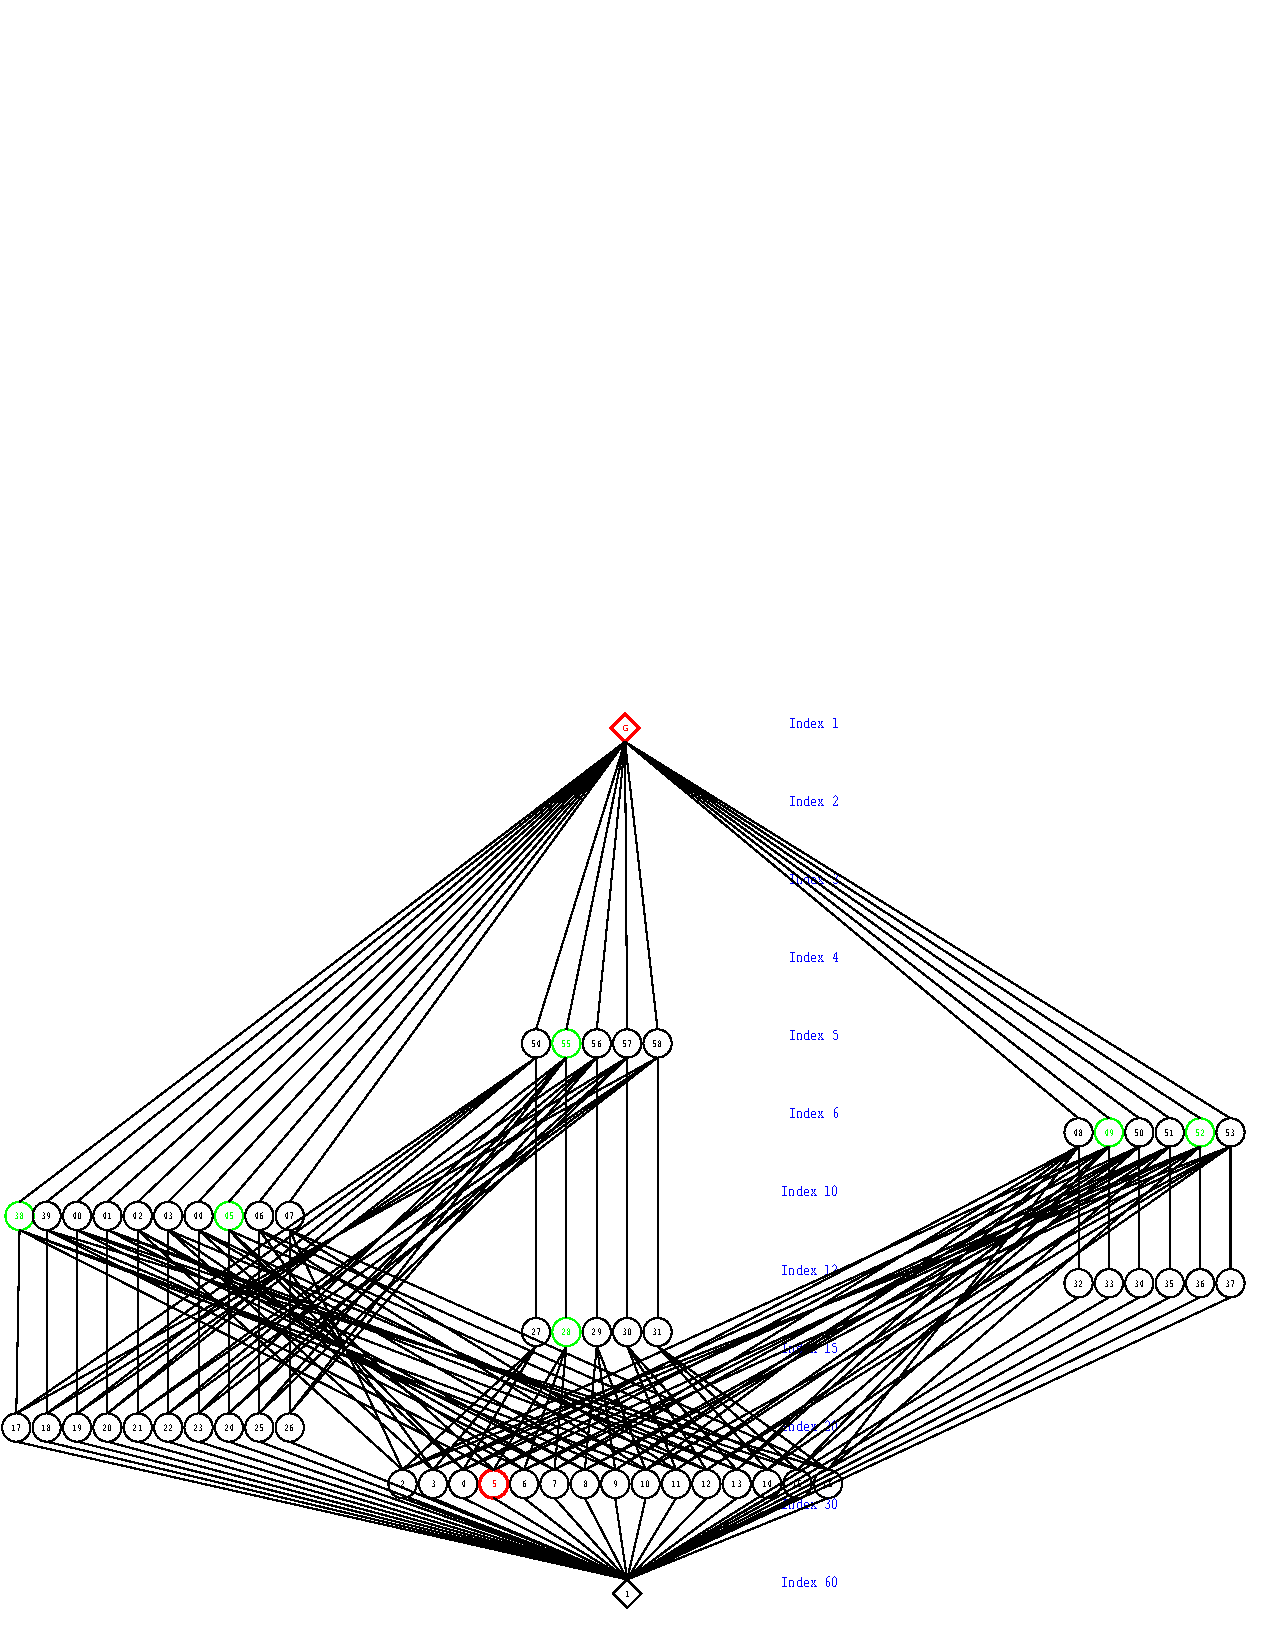
\includegraphics[height=15cm]{A5UpperN5.pdf}%
\caption{Hasse diagram of $\Sub[A_5]$ drawn by the \xgap\ program. Colored green are the
subgroups in the interval above one of the $\Z_2$ subgroups of $A_5$.  Thus,
$A_5$ acts transitively on the 30 cosets of $\Z_2$, and the
permutational algebra $\<A_5/\Z_2; A_5\>$ has congruence lattice isomorphic to 
the interval $[\Z_2, A_5]$.}
\label{fig:A5new}
\end{center}
\end{figure}

If we use the \xgap\ program as described above we could count the conjugacy classes of subgroups by
looking at the Hasse diagram of $\Sub[A_5]$.  However, it's more convenient (and
faster) to simply do: 
{\codesize 
\begin{verbatim}
gap> ccsg := ConjugacyClassesSubgroups( a5 );;
gap> Size(ccsg);
\end{verbatim}}
\noindent which returns 9, telling us that $A_5$ has 9 conjugacy classes of subgroups.  
This includes the singleton classes $\{(e)\}$ and $\{A_5\}$,
which \gap\ calls \verb!Group( () )^G! and \verb!AlternatingGroup( [ 1 .. 5 ] )^G!,
respectively. 
Let's examine the other seven classes.  We get a list of representative subgroups, one for
each class, as follows:
{\codesize 
\begin{verbatim}

gap> clreps := List( ccsg, x -> Representative( x ));
[ Group(()), Group([ (2,3)(4,5) ]), Group([ (3,4,5) ]), 
  Group([ (2,3)(4,5), (2,4)(3,5) ]), Group([ (1,2,3,4,5) ]), 
  Group([ (3,4,5), (1,2)(4,5) ]), Group([ (1,2,3,4,5), (2,5)(3,4) ]), 
  Group([ (2,3)(4,5), (2,4)(3,5), (3,4,5) ]), Alt( [ 1 .. 5 ] ) ]

\end{verbatim}}
\noindent The orders and indices of these subgroups are given by
{\codesize 
\begin{verbatim}

gap> List( clreps, x -> Order(x));         
     % returns [ 1, 2, 3, 4, 5, 6, 10, 12, 60 ]
gap> List( clreps, x -> Index( a5, x ) );  
     % returns [ 60, 30, 20, 15, 12, 10, 6, 5, 1 ]

\end{verbatim}}
\noindent (Of course, any subgroup $H\leq A_5$ has order $|H| = |A_5|\,[A_5:H] = 60 \,[A_5:H]$.)  
From the list of subgroup orders, we see that {\tt clreps[2]}, {\tt clreps[3]},
and {\tt clreps[5]} must be the groups $\Z_2$, $\Z_3$, and $\Z_5$ (the only groups of 
orders two, three, and five, respectively).  
We can easily identify the other subgroups as well.\footnote{A
  nice reference list of all groups of orders 1 through 15 is given on pp.~98--9 of
  Hungerford~\cite{Hungerford:1974}.} 
For example, {\tt clreps[4]} has order 4, so it must be either 
$\Z_2 \oplus \Z_2$ or $\Z_4$.  Deciding to which isomorphism class {\tt clreps[4]}
belongs is simply a matter of checking whether it's cyclic.  These and other
subgroups can be determined using the following \gap\ commands:
% {\tt IsCyclic}, {\tt IsAbelian}, {\tt IsDihedralGroup}, {\tt IsAlternatingGroup}; e.g.
{\codesize 
\begin{verbatim}

gap> IsCyclic( clreps[4] );            # returns false
gap> IsAbelian( clreps[6] );           # returns false
gap> IsDihedralGroup( clreps[6] );     # returns true
gap> IsDihedralGroup( clreps[7] );     # returns true
gap> IsAlternatingGroup( clreps[8] );  # returns true

\end{verbatim}}
\noindent Therefore, {\tt clreps[4]} must be the Klein four group $\Z_2 \oplus
\Z_2$, {\tt clreps[6]} must be $D_3$, 
{\tt clreps[7]}  must be $D_5$.  Finally, {\tt clreps[8]} has
order 12, so it must be one of $\Z_2 \oplus \Z_{6}$, $\Z_{12}$, $A_4$,
$D_6$, or %$T$.
the group $T$ (generated by two elements $a, b$ where $|a|=6, b^2 = a^3$, and $ba = a^{-1}b$).  
The last command above shows that {\tt clreps[8]} is $A_4$.

The foregoing demonstrates some useful \gap\ commands, but we could have
identified all these subgroups in one step with the {\tt StructureDescription} command:
{\codesize 
\begin{verbatim}

gap> List(clreps, x->StructureDescription(x));
[ "1", "C2", "C3", "C2 x C2", "C5", "S3", "D10", "A4", "A5" ]

\end{verbatim}}

Now, the representations of $A_5$ are all faithful since $A_5$ is simple.  Below is
a table of all seven (equivalence classes of) permutation representations of
$A_5$ on cosets $A_5/H$, ordered by the number of such cosets (i.e.~the index
$[A_5:H]$): \\
{\small
  \begin{center}
\begin{tabular}{c|c|c|c}
%Conjugacy class & Index & & \\
  Conjugacy & Index & &  \\
   class rep.~$H$   & $[A_5: H]$ & Representation homomorphism & Is it primitive?\\
\hline
$A_4$ &  5 & $\rho_{A_4}  : A_5 \hookrightarrow \Sym(A_5/A_4) \cong S_5$ & yes \\
$D_5$ &  6 & $\rho_{D_5}  : A_5 \hookrightarrow \Sym(A_5/D_5) \cong S_6$ & yes \\
$D_3$ & 10 & $\rho_{D_3}  : A_5 \hookrightarrow \Sym(A_5/D_3) \cong S_{10}$ & yes \\
$\Z_5$& 12 & $\rho_{\Z_5} : A_5 \hookrightarrow \Sym(A_5/\Z_5) \cong S_{12}$ & no\\
$V_4$ & 15 & $\rho_{V_4}  : A_5 \hookrightarrow \Sym(A_5/V_4) \cong S_{15}$ & no\\
$\Z_3$& 20 & $\rho_{\Z_3} : A_5 \hookrightarrow \Sym(A_5/\Z_3) \cong S_{20}$ & no\\
$\Z_2$& 30 & $\rho_{\Z_2} : A_5 \hookrightarrow \Sym(A_5/\Z_2) \cong S_{30}$ & no\\
$(e)$& 60 & $\rho : A_5 \hookrightarrow \Sym(A_5) \cong S_{60}$ & no\\
\hline
\end{tabular}
  \end{center}
  }
~\\[4pt]
We can use \gap\ to verify that $A_5$ does indeed show up as a transitive
subgroup of some of the symmetric groups listed in the table above.  For
example, the first two are checked as follows:
{\codesize 
\begin{verbatim}

gap> NrTransitiveGroups(5);  % returns 5
gap> NrTransitiveGroups(6);  % returns 16
gap> List([1..5], x->StructureDescription(TransitiveGroup(5,x)));
[ "C5", "D10", "C5 : C4", "A5", "S5" ]
gap> List([1..16], x->StructureDescription(TransitiveGroup(6,x)));
[ "C6", "S3", "D12", "A4", "C3 x S3", "C2 x A4", "S4", "S4", "S3 x S3", 
  "(C3 x C3) : C4", "C2 x S4", "A5", "(S3 x S3) : C2", "S5", "A6", "S6" ]

\end{verbatim}}
\noindent The last line above indicates that (some copy of) $A_5$ shows up as a transitive
subgroup of $S_6$.  (Of course, it is \emph{not} the copy of $A_5< S_6$ that
moves only five points!) 

The last column of the table above was filled in simply 
by looking at the subgroup lattice of $A_5$ in~Figure~\ref{fig:A5new}.  
In general, if $H$ is a coatom in $\Sub[G]$ (i.e.~a maximal subgroup of $G$),
then the representation  
\[
\rho_{H} : G \rightarrow \Sym(G/H) \cong S_{[G:H]}
\] is primitive.
\\[10pt]
{\bf G-sets.} Defining G-sets with \gap\ is very useful and important.  It allows us to work
with and analyze a particular permutation representation.  Let us consider the
$A_5$-set given by $A_5$ acting on cosets of $H=$ {clreps[2]} $=C_2$. In \gap\
we do
{\codesize 
\begin{verbatim}

gap> G := AlternatingGroup( 5 );;
gap> ccsg := ConjugacyClassesSubgroups( a5 );;
gap> H := Representative( ccsg[3] );                   # C3
gap> Gbar := Action( G, RightCosets(G,H), OnRight );;  # a subgroup of S20 
                                                       # isomorphic to A5
gap> MovedPoints( Gbar );                              # [ 1, ..., 20 ]
gap> AllBlocks( Gbar );    # [ [ 1, 2, 3, 4 ], [ 1, 6, 11, 16 ], [ 1, 20 ] ]
gap> for b in AllBlocks( Gbar ) do Print( Orbit( Gbar, b, OnSets ), "\n"); od;
\end{verbatim}}
{\scriptsize 
\begin{verbatim}
[ [ 1, 2, 3, 4 ], [ 17, 18, 19, 20 ], [ 13, 14, 15, 16 ], [ 9, 10, 11, 12 ], [ 5, 6, 7, 8 ] ]
[ [ 1, 6, 11, 16 ], [ 2, 7, 12, 17 ], [ 3, 8, 13, 18 ], [ 4, 9, 14, 19 ], [ 5, 10, 15, 20 ] ]
[ [ 1, 20 ], [ 16, 17 ], [ 12, 13 ], [ 11, 18 ], [ 8, 9 ], [ 7, 14 ], [ 6, 19 ], ...
  ..., [ 4, 5 ], [ 3, 10 ], [ 2, 15 ] ]

\end{verbatim}}
\noindent The command {\tt MovedPoints} shows that {\tt Gbar} $\cong A_5$ acts transitively on the set
$G/H = A_5/Z_3$ of 30 cosets.  (We could also have checked that the action is transitive
using {\tt Orbits(Gbar)} and noting that there is just one orbit.)
The command {\tt AllBlocks(Gbar)} shows 
the first block of each nontrivial ``system of imprimitivity'' (or congruence) of
the G-set $\<G/H, \bar{G}\>$.  Finally, the last command displays the three
nontrivial congruences, and shows $\Con \<G/H, \bar{G}\>\cong M_3$.  Another way
to see that  $\Con \<G/H, \bar{G}\>\cong M_3$ is to check the sublattice of
intermediate subgroups between $H$ and $G$, as follows:
{\codesize 
\begin{verbatim}
gap> intHG := IntermediateSubgroups(G, H);
\end{verbatim}}
{\codesize
\begin{verbatim}
rec( subgroups := [ Group([(3,4,5), (1,2)(4,5)]), Group([(3,4,5), (2,3)(4,5)]), 
                    Group([(3,4,5), (1,5,3)]) ], 
     inclusions := [[ 0, 1 ], [ 0, 2 ], [ 0, 3 ], [ 1, 4 ], [ 2, 4 ], [ 3, 4 ]] 
   )
\end{verbatim}}
\noindent This results in an object, which I've called {\tt intHG}, having fields
{\tt intHG.subgroups} and {\tt intHG.inclusions}.  The inclusions field shows
the covering relations in the sublattice interval $[H, G] \leq \Sub[G]$.

  % \\[6pt]
% {\bf A more general example.}  The example above was special because $A_5$ is a
% simple group.  In general, given a finite group $G$, and an arbitrary subgroup
% $H$, the representation $\rho_H$ need not be an embedding of $G$ into
% $\Sym(G/H)$.  



\subsection{The Symmetric Group on Four Letters}

The symmetric group on four letters, $S_4$, contains the following permutations:
\begin{center}
\begin{tabular}{|c|c|}
\hline
permutations & type\\[4pt]
\hline
(01), (02), (03), (12), (13), (23) & 2-cycles \\[4pt]
(01)(23), (02)(13), (03)(12) & product of 2-cycles \\[4pt]
(012), (013), (021), (023), (031), (032), (123), (132) &  3-cycles \\[4pt]
(0123), (0132), (0213), (0231), (0312), (0321) & 4-cycles \\[4pt]
\hline
\end{tabular}
\end{center}

Within each row of the table, the elements are listed in lexicographic order.  We might
use this ordering as a guide when assigning the labels $\{0, 1, 2, \ldots, 23\}$ to
the elements of $S_4$.  For example, one possible labelling 
(which assigns even numbers to $A_4$) is shown in the table on the following page.
\\

{\scriptsize
\begin{tabular}{|l|c|c|c|c|c|c|c|c|c|}
\hline
label& 0&1& 2& 3& 4& 5& 6& 7& 8\\
\hline
element&
 e &
(01)&
(01)(23)&
(02)&
(02)(13)&
(03)&
(03)(12)&
(12)&
(012)\\
\hline
\end{tabular}
}

{\scriptsize
\begin{tabular}{|l|c|c|c|c|c|c|c|c|}
\hline
label & 9& 10& 11& 12& 13& 14& 15& 16\\
\hline
element &(13)&(013)& (23)&(021)&(0123)&(023)&(0132)&(031)\\
\hline
\end{tabular}
}

{\scriptsize
\begin{tabular}{|l|c|c|c|c|c|c|c|}
\hline
label& 17& 18& 19& 20& 21& 22& 23\\
\hline
element &(0213)&(032)&(0231)&(123)&(0312)&(132)&(0321)\\
\hline
\end{tabular}
}

\newpage
There are 30 subgroups of $S_4$. The following table presents
them all, except $(e)$ and $S_4$, and their element labels:

{\footnotesize
\begin{center}
\begin{tabular}{|r|c|c|c|c|}
\hline
&name & elements & element labels & order\\
\hline
0& $A_4$ & $\{e, (01)(23), (02)(13), (03)(12),(012), (013), \ldots$& $\{0,2, 4, 6,\ldots, 22\}$ & 12\\[4pt]
 &       & $\ldots, (021), (023), (031), (032), (123), (132)\}$  &  &\\[4pt]
\hline
1&$V_4$ & $\{e, (01)(23), (02)(13), (03)(12)\}$ & $\{0,2,4,6\}$& 4\\[4pt]
\hline
2&$v_0,\, v_1, \,v_2$ & $\{e, (01)(23)\},\; \{e, (02)(13)\}, \; \{e, (03)(12)\}$ & $\{0,2\},
\{0,4\}, \{0,6\}$& 2, 2, 2\\[4pt]
\hline
5& $P_0$ & $\{e, (012), (021)\}$ &$\{0,8,12\}$& 3\\[4pt]
\hline
6&$P_1$ & $\{e, (013), (031)\}$ &$\{0,10,16\}$& 3\\[4pt]
\hline
7&$P_2$ & $\{e, (023), (032)\}$ &$\{0,14,18\}$& 3\\[4pt]
\hline
8&$P_3$ & $\{e, (123), (132)\}$ &$\{0,20,22\}$& 3\\[4pt]
\hline
9&$D$ & $\{e, (01),(01)(23), (02)(13), \dots$ & $\{0,1,2,4,6,11,17,21\}$& 8\\[4pt]
& & \phantom{XXX} $\dots, (03)(12), (23), (0213), (0312)\}$ & & \\[4pt]
\hline
10&$d$ & $\{e, (01)(23), (0213), (0312)\}$ & $\{0,2,17,21\}$& 4\\[4pt]
\hline
11&$D'$ & $\{e, (01)(23), (02), (02)(13), \dots $&$\{0,2,3,4,6,9,13,23\}$& 8\\[4pt]
& & \phantom{XXX} $\dots, (03)(12), (13), (0123), (0321)\}$     && \\[4pt]
\hline
12&$d'$ & $\{e, (02)(13), (0123), (0321)\}$ &$\{0,4,13,23\}$& 4\\[4pt]
\hline
13&$D''$ & $\{e, (01)(23), (02)(13), \dots $ &$\{0,2,4,5,6,7,15,19\}$& 8\\[4pt]
& &  \phantom{XXX} $\dots, (03), (03)(12), (12), (0132), (0231)\}$ &&\\[4pt]
\hline
14&$d''$ & $\{e, (03)(12), (0132), (0231)\}$ &$\{0,6,15,19\}$& 4\\[4pt]
\hline
15&$H_0$ & $\{e, (01), (02), (12), (012), (021)\}$ & $\{0, 1, 3, 7, 8, 12\}$& 6\\[4pt]
\hline
16&$H_1$ & $\{e, (01), (03), (13), (013), (031)\}$ & $\{0, 1, 5, 9, 10, 16\}$& 6\\[4pt]
\hline
17&$H_2$ & $\{e, (02), (03), (23), (023), (032)\}$ & $\{0, 3, 5, 11, 14, 18\}$& 6\\[4pt]
\hline
18&$H_3$ & $\{e, (12), (13), (23), (123), (132)\}$ & $\{0, 7, 9, 11, 20, 22\}$& 6\\[4pt]
\hline
19&$A$ & $\{e, (01),(01)(23),(23) \}$ & $\{0, 1, 2, 11\}$& 4 \\[4pt]
\hline
20&$a_0,\, a_1$ & $\{e, (01)\}, \; \{e, (23) \}$ & $\{0, 1\}, \;\{0, 11\}$& 2, 2 \\[4pt]
\hline
22&$B$ & $\{e, (02), (02)(13),(13)\}$ & $\{0, 3, 4, 9\}$& 4 \\[4pt]
\hline
23&$b_0,\, b_1$ & $\{e, (02)\}, \; \{e, (13)\}$ & $\{0, 3\}, \, \{0, 9\}$& 2, 2 \\[4pt]
\hline
25&$C$ & $\{e, (03), (03)(12), (12)\}$ & $\{0, 5, 6, 7\}$& 4 \\[4pt]
\hline
26&$c_0, \, c_1$ & $\{e, (03)\}, \; \{e, (12)\}$ & $\{0, 5\}, \, \{0, 7\}$& 2, 2 \\[4pt]
\hline
\end{tabular}
\end{center}
}
\newpage
Let $X = \{0, 1, 2, \ldots, 23\}$.  
If you stare long enough at the table of subgroups on the previous page, it becomes apparent
how we can construct partitions in $\Eq(X)$ using cosets of the appropriate subgroups
in such a way that the resulting equivalences generate a sublattice isomorphic to
$\Eq(4)$. Specifically, look at $A, B, C$, and $H_i \; (i=0,1,2,3)$, and the
subgroups below them, and notice how their intersections resemble the meet 
structure of $\Eq(4)$.  

Let $\delta_i$ be the equivalence constructed from the cosets of $H_i$.  From the
previous observation concerning the meet structure, it is clear that the
four equivalences $\delta_i \; (i=0,1,2,3)$ will serve as the four generating
coatoms of the $\Eq(4)$ sublattice.  Thus, we need only construct these four
equivalences, and let them generate the rest of the $\Eq(4)$ sublattice.
(Though we might verify that three of the coatoms they generate correspond to
the equivalences we would get using cosets of $A, B$, and $C$.)

The cosets of $H_i$, and the resulting partitions $\delta_i$, are shown on the
next page. 
%% ~\\
%% \vspace{-15mm}
{\small
  \[
H_0 = \{e, (01), (02), (12), (012), (021)\} = \{0, 1, 3, 7, 8, 12\}
\]
\[
H_0(03) = \{(03), (031), (032), (03)(12), (0312), (0321)\} = \{5,6,16,18,21,23\}
\]
\[
H_0(13) = \{(13), (013), (02)(13), (132), (0132), (0213)\} = \{4,9,10,15,17,22\}
\]
\[
H_0(23) = \{(23), (01)(23), (023), (123), (0123), (0231)\} = \{2,11,13,14,20,19\}
\]
Define $\delta_0 = (H_0|H_0(03)|H_0(13)|H_0(23))$. That is,
\[
\delta_0 = (0, 1, 3, 7, 8, 12|5,6,16,18,21,23|4,9,10,15,17,22|2,11,13,14,20,19)
\]
Similarly,
\[
H_1 = \{e, (01), (03), (13), (013), (031)\} = \{0, 1, 5, 9, 10, 16\}
\]
\[
H_1(02) = \{(02), (021), (023), (02)(13), (0213), (0231)\} = \{3, 4, 12, 14, 17, 19\}
\]
\[
H_1(12) = \{(12), (012), (03)(12), (123), (0123), (0312)\} = \{6, 7, 8, 13, 20, 21\}
\]
\[
H_1(23) = \{(23), (01)(23), (032), (132), (0132), (0321)\} = \{2, 11, 15, 18, 22, 23\}
\]
\[
\delta_1 = (0, 1, 5, 9, 10, 16|3, 4, 12, 14, 17, 19|6, 7, 8, 13, 20, 21|2, 11, 15, 18, 22, 23)
\]
\[
H_2 = \{e, (02), (03), (23), (023), (032)\} = \{0, 3, 5, 11, 14, 18\}
\]
\[
H_2(01) = \{(01), (012), (013), (01)(23), (0123), (0132)\} = \{1,2,8,10,13,15\}
\]
\[
H_2(12) = \{(12), (021), (03)(12), (132), (0213), (0321)\} = \{6,7,12,17,22,23\}
\]
\[
H_2(13) = \{(13), (02)(13), (031), (123), (0231), (0312)\} = \{4,9,16,20,19,21\}
\]
\[
\delta_2 = (0,3,5,11,14,18|1,2,8,10,13,15|6,7,12,17,22,23|4,9,16,20,19,21)
\]
\[
H_3 = \{e, (12), (13), (23), (123), (132)\} = \{0, 7, 9, 11, 20, 22\}
\]
\[
H_3(01) = \{(01), (021), (031), (01)(23), (0231), (0321)\} = \{1,2,12,16,19,23\}
\]
\[
H_3(02) = \{(02), (012), (02)(13), (032), (0312), (0132)\} = \{3,4,8,15,18,21\}
\]
\[
H_3(03) = \{(03), (03)(12), (013), (023), (0123), (0213)\} = \{5,6,10,13,14,17\}
\]
\[
\delta_3 = (0,7,9,11,20,22|1,2,12,16,19,23|3,4,8,15,18,21|5,6,10,13,14,17).
\]
}

\newpage
Let $L\leq \Eq(X)$ denote the lattice generated by $\delta_i\;(i=0,1,2,3)$. 
Our computer programs identify the unary operations on $X$ which respect all four 
equivalences $\delta_i\;(i=0,1,2,3)$.  There are 48 such operations, 
so $|\lambda(L)| = 48$.  Leaving out the 24 constant maps, the
remaining 23 operations appear below:
{\small
\begin{verbatim}
 0  1  2  3  4  5  6  7  8  9 10 11 12 13 14 15 16 17 18 19 20 21 22 23
 1  0 11  8 21 10 17 12  3 16  5  2  7 14 13 18  9  6 15 20 19  4 23 22
 2 11  0 13  6 15  4 19 14 23 18  1 20  3  8  5 22 21 10  7 12 17 16  9
 3 12 23  0  9 14 13  8  7  4 17 18  1  6  5 22 19 10 11 16 21 20 15  2
 4 17  6  9  0 19  2 15 22  3 12 21 10 23 16  7 14  1 20  5 18 11  8 13
 5 16 19 18 15  0  7  6 21 10  9 14 23 20 11  4  1 22  3  2 13  8 17 12
 6 21  4 23  2  7  0  5 16 13 20 17 18  9 22 19  8 11 12 15 10  1 14  3
 7  8 15 12 19  6  5  0  1 20 13 22  3 10 17  2 21 14 23  4  9 16 11 18
 8  7 22  1 16 13 14  3 12 21  6 15  0 17 10 23 20  5  2  9  4 19 18 11
 9 10 13  4  3 16 23 22 15  0  1 20 17  2 19  8  5 12 21 14 11 18  7  6
10  9 20 15 18  1 12 17  4  5 16 13 22 19  2 21  0 23  8 11 14  3  6  7
11  2  1 14 17 18 21 20 13 22 15  0 19  8  3 10 23  4  5 12  7  6  9 16
12  3 18  7 20 17 10  1  0 19 14 23  8  5  6 11  4 13 22 21 16  9  2 15
13 20  9  2 23  8  3 14 19  6 21 10 11  4 15 16  7 18  1 22 17 12  5  0
14 19 16 11 22  3  8 13 20 17  4  5  2 21 18  9 12 15  0 23  6  7 10  1
15 22  7 10  5  2 19  4 17 18 23  8  9 12  1  6 11 16 13  0  3 14 21 20
16  5 14 21  8  9 22 23 18  1  0 19  6 11 20  3 10  7  4 13  2 15 12 17
17  4 21 22 11 12  1 10  9 14 19  6 15 16 23 20  3  2  7 18  5  0 13  8
18 23 12  5 10 11 20 21  6 15 22  3 16  7  0 17  2  9 14  1  8 13  4 19
19 14  5 20  7  4 15  2 11 12  3 16 13 18 21  0 17  8  9  6 23 22  1 10
20 13 10 19 12 21 18 11  2  7  8  9 14 15  4  1  6  3 16 17 22 23  0  5
21  6 17 16  1 20 11 18 23  8  7  4  5 22  9 12 13  0 19 10 15  2  3 14
22 15  8 17 14 23 16  9 10 11  2  7  4  1 12 13 18 19  6  3  0  5 20 21
23 18  3  6 13 22  9 16  5  2 11 12 21  0  7 14 15 20 17  8  1 10 19  4
\end{verbatim}
}
\newpage
The lattice $L\cong \Eq(4)$ has 15 elements, while the closure of $L$ in $\Eq(X)$ has
30 elements.  Besides the all relation and the zero relation, the closure of $L$
consists of the following congruences (the elements of $L$ are identified by *):

{\small
\begin{verbatim}
 |0,1,2,4,6,11,17,21|3,9,10,12,13,18,20,23|5,7,8,14,15,16,19,22| D
*|0,1,2,11|3,12,18,23|4,6,17,21|5,14,16,19|7,8,15,22|9,10,13,20| A
*|0,1,3,7,8,12|2,11,13,14,19,20|4,9,10,15,17,22|5,6,16,18,21,23| H_0
*|0,1,5,9,10,16|2,11,15,18,22,23|3,4,12,14,17,19|6,7,8,13,20,21| H_1
*|0,1|2,11|3,12|4,17|5,16|6,21|7,8|9,10|13,20|14,19|15,22|18,23| a_0
 |0,2,3,4,6,9,13,23|1,8,11,14,16,17,21,22|5,7,10,12,15,18,19,20| D'
 |0,2,4,6,8,10,12,14,16,18,20,22|1,3,5,7,9,11,13,15,17,19,21,23| A_4
 |0,2,4,5,6,7,15,19|1,10,11,12,17,18,20,21|3,8,9,13,14,16,22,23| D''
 |0,2,4,6|1,11,17,21|3,9,13,23|5,7,15,19|8,14,16,22|10,12,18,20| V_4
 |0,2,17,21|1,4,6,11|3,10,20,23|5,8,19,22|7,14,15,16|9,12,13,18| d
 |0,2|1,11|3,23|4,6|5,19|7,15|8,22|9,13|10,20|12,18|14,16|17,21| v_0
*|0,3,5,11,14,18|1,2,8,10,13,15|4,9,16,19,20,21|6,7,12,17,22,23| H_2
*|0,7,9,11,20,22|1,2,12,16,19,23|3,4,8,15,18,21|5,6,10,13,14,17| H_3
*|0,11|1,2|3,18|4,21|5,14|6,17|7,22|8,15|9,20|10,13|12,23|16,19| a_1
*|0,3,4,9|1,8,16,21|2,6,13,23|5,10,15,18|7,12,19,20|11,14,17,22| B
*|0,3|1,8|2,13|4,9|5,18|6,23|7,12|10,15|11,14|16,21|17,22|19,20| b_0
 |0,8,12|1,3,7|2,14,20|4,10,22|5,21,23|6,16,18|9,15,17|11,13,19| P_0
 |0,4,13,23|1,14,21,22|2,3,6,9|5,12,15,20|7,10,18,19|8,11,16,17| d'
 |0,4|1,21|2,6|3,9|5,15|7,19|8,16|10,18|11,17|12,20|13,23|14,22| v_1
*|0,5,6,7|1,10,12,17|2,4,15,19|3,8,13,14|9,16,22,23|11,18,20,21| C
 |0,6,15,19|1,17,18,20|2,4,5,7|3,13,16,22|8,9,14,23|10,11,12,21| d''
 |0,6|1,17|2,4|3,13|5,7|8,14|9,23|10,12|11,21|15,19|16,22|18,20| v_2
*|0,9|1,16|2,23|3,4|5,10|6,13|7,20|8,21|11,22|12,19|14,17|15,18| b_1
*|0,5|1,10|2,15|3,14|4,19|6,7|8,13|9,16|11,18|12,17|20,21|22,23| c_0
 |0,10,16|1,5,9|2,18,22|3,17,19|4,12,14|6,8,20|7,13,21|11,15,23| P_1
 |0,14,18|1,13,15|2,8,10|3,5,11|4,16,20|6,12,22|7,17,23|9,19,21| P_2
*|0,7|1,12|2,19|3,8|4,15|5,6|9,22|10,17|11,20|13,14|16,23|18,21| c_1
 |0,20,22|1,19,23|2,12,16|3,15,21|4,8,18|5,13,17|6,10,14|7,9,11| P_3
\end{verbatim}
}
\newpage
The cosets of the subgroups $A, B$, and $C$ should\footnote{I haven't checked carefully that these are actually the cosets.}
correspond to the following partitions:
\[
\alpha = (0,1,2,11|3,12,18,23|4,6,17,21|5,14,16,19|7,8,15,22|9,10,13,20)
\]
\[
\beta = (0,3,4,9|1,8,16,21|2,6,13,23|5,10,15,18|7,12,19,20|11,14,17,22)
\]
\[
\gamma = (0,5,6,7|1,10,12,17|2,4,15,19|3,8,13,14|9,16,22,23|11,18,20,21)
\]
These equivalences are the ``non-generating'' coatoms of $L$.  
They generate an $M_3$ sublattice, and each is above two atoms 
(unlike the ``generating'' coatoms $\delta_i$, each of which covers three atoms).  
The six atoms of $L$ are marked on the previous page by $a_i, b_i, c_i \, (i=0,1)$.  They are as follows:
{\scriptsize
\[
a_0 = \alpha \meet \delta_0 = \alpha\meet \delta_1 = (0,1|2,11|3,12|4,17|5,16|6,21|7,8|9,10|13,20|14,19|15,22|18,23)
\]
\[
a_1 = \alpha \meet \delta_2 = \alpha\meet \delta_3 = (0,11|1,2|3,18|4,21|5,14|6,17|7,22|8,15|9,20|10,13|12,23|16,19)
\]
\[
b_0 = \beta \meet \delta_0 = \beta \meet \delta_2 = (0,3|1,8|2,13|4,9|5,18|6,23|7,12|10,15|11,14|16,21|17,22|19,20)
\]
\[
b_1 =\beta \meet \delta_1 = \beta\meet \delta_3 = (0,9|1,16|2,23|3,4|5,10|6,13|7,20|8,21|11,22|12,19|14,17|15,18)
\]
\[
c_0 =\gamma \meet \delta_1 = \gamma \meet \delta_2 = (0,5|1,10|2,15|3,14|4,19|6,7|8,13|9,16|11,18|12,17|20,21|22,23)
\]
\[
c_1 =\gamma \meet \delta_0 = \gamma \meet \delta_3 = (0,7|1,12|2,19|3,8|4,15|5,6|9,22|10,17|11,20|13,14|16,23|18,21)
\]
}
We could try to prove that the closure of such
``uniform'' embeddings of $\Eq(n)$ in $\Eq(n!)$ should always contain the congruence 
corresponding to the cosets of $A_n$. 
In light of the foregoing data, we might try to prove some or all of the
following, for every uniform embedding of $\Eq(4)\cong L \leq \Eq(X)$:
\begin{enumerate}[(i)]
\item $|X|\geq 24$
\item $\forall \alpha \in L \setminus \{1\}$ the block size of $\alpha$ is strictly
  less than $|X|/2$
\item $L$ does not contain the partition corresponding to cosets of $A_n$
\item the closure of $L$ contains the partition corresponding to cosets of $A_n$
\item the closure of $L$ contains an element with block size $|X|/2$
\end{enumerate}
Item (i) is easily within reach, and (ii) and (iii) seem plausible. 
Of course,% (ii) implies (iii), and (iv) implies (v).  
if both (ii) and (v) hold, or both (iii) and (iv) hold, the FLRP is solved.


%% \subsection{Subgroups of the Symmetric Group on Four Letters}
%% 
The symmetric group on four letters, $S_4$, contains the following permutations:

\begin{center}
\begin{tabular}{|c|c|}
\hline
permutations & type\\[4pt]
\hline
(12), (13), (14), (23), (24), (34) & 2-cycles \\[4pt]
(12)(34), (13)(24), (14)(23) & product of 2-cycles \\[4pt]
(123), (124), (132), (134), (142), (143), (234), (243) &  3-cycles \\[4pt]
(1234), (1243), (1324), (1342), (1423), (1432) & 4-cycles \\[4pt]
\hline
\end{tabular}
\end{center}

\begin{figure}[!ht]
\vspace{-9cm}
\hskip-1.5cm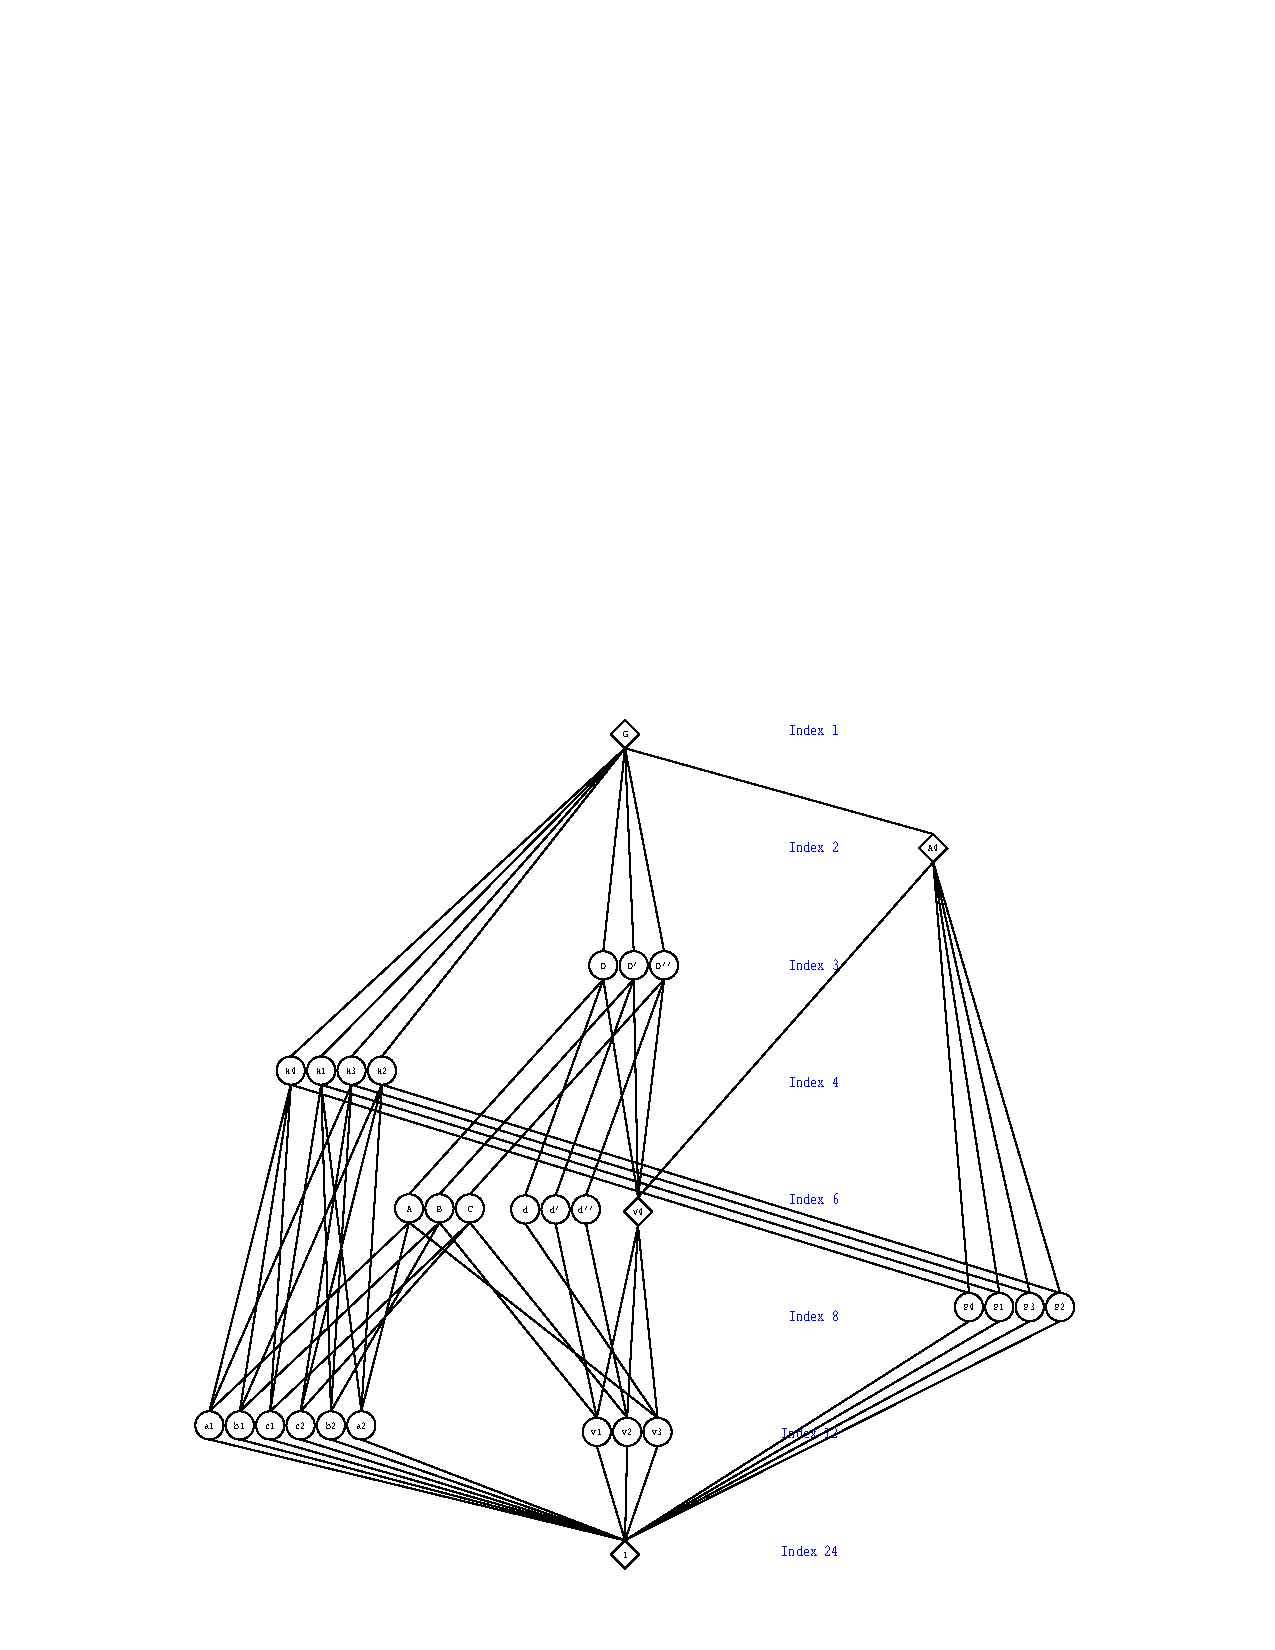
\includegraphics[height=20cm]{SubS4morelabels.pdf}%
\caption{Hasse diagram of $\Sub[S_4]$ drawn by the XGAP program.}
\label{fig:SubS4}
\end{figure}

~
\vfill

\newpage

{\footnotesize
    \begin{table}[h!]
      \centering
      \caption{There are 30 subgroups of $S_4$; all 
        except $(e)$ and $S_4$ are displayed here.}
      \begin{tabular}{|c|c|c|c|}
        \hline
        label & elements & order& isomorphic to\\
\hline
$A_4$ & $\{e, (12)(34), (13)(24), (14)(23),(123), (124), \ldots$& 12 & $A_4$\\[4pt]
      & $\ldots, (132), (134), (142), (143), (234), (243)\}$  & &\\[4pt]
\hline
$V_4$ & $\{e, (12)(34), (13)(24), (14)(23)\}$ & 4& $V_4$\\[4pt]
\hline
$v_1,\, v_2, \,v_3$ & $\{e, (12)(34)\},\; \{e, (13)(24)\}, \; \{e, (14)(23)\}$ & 2, 2, 2& $Z_2$\\[4pt]
\hline
$P_1$ & $\{e, (123), (132)\}$ & 3& $Z_3$\\[4pt]
\hline
$P_2$ & $\{e, (124), (142)\}$ & 3& $Z_3$\\[4pt]
\hline
$P_3$ & $\{e, (134), (143)\}$ & 3& $Z_3$\\[4pt]
\hline
$P_4$ & $\{e, (234), (243)\}$ & 3& $Z_3$\\[4pt]
\hline
$D$ & $\{e, (12),(12)(34), (13)(24), (14)(23), (34), (1324), (1423)\}$ & 8& $D_4$\\[4pt]
\hline
$d$ & $\{e, (12)(34), (1324), (1423)\}$ & 4& $Z_4$\\[4pt]
\hline
$D'$ & $\{e, (12)(34), (13), (13)(24), (14)(23), (24), (1234), (1432)\}$ & 8& $D_4$\\[4pt]
\hline
$d'$ & $\{e, (13)(24), (1234), (1432)\}$ & 4& $Z_4$\\[4pt]
\hline
$D''$ & $\{e, (12)(34), (13)(24), (14), (14)(23), (23), (1243), (1342)\}$ & 8& $D_4$\\[4pt]
\hline
$d''$ & $\{e, (14)(23), (1243), (1342)\}$ & 4& $Z_4$\\[4pt]
\hline
$H_1$ & $\{e, (12), (13), (23), (123), (132)\}$ & 6& $S_3$\\[4pt]
\hline
$H_2$ & $\{e, (12), (14), (24), (124), (142)\}$ & 6& $S_3$\\[4pt]
\hline
$H_3$ & $\{e, (13), (14), (34), (134), (143)\}$ & 6& $S_3$\\[4pt]
\hline
$H_4$ & $\{e, (23), (24), (34), (234), (243)\}$ & 6& $S_3$\\[4pt]
\hline
$A$ & $\{e, (12),(12)(34),(34) \}$ & 4& $V_4$\\[4pt]
\hline
$a_1,\, a_2$ & $\{e, (12)\}, \; \{e, (34) \}$ & 2, 2& $Z_2$\\[4pt]
\hline
$B$ & $\{e, (13), (13)(24),(24)\}$ & 4& $V_4$\\[4pt]
\hline
$b_1,\, b_2$ & $\{e, (13)\}, \; \{e, (24)\}$ & 2, 2& $Z_2$\\[4pt]
\hline
$C$ & $\{e, (14), (14)(23), (23)\}$ & 4& $V_4$\\[4pt]
\hline
$c_2, \, c_1$ & $\{e, (14)\}, \; \{e, (23)\}$ & 2, 2& $Z_2$\\[4pt]
\hline
      \end{tabular}
    \end{table}
}


\newpage

\section{Decompositions}
\subsection{Subdirect Products}
In this section we discuss a theorem about subgroups of direct products of
groups, and describe a consequence for subdirect powers of finite nonabelian
simple groups.  The theorem is a slight generalization of a well-known result
due to Remak, Klein, and Fricke (cf.~Rose~\cite{Rose:1978}, Theorem 
8.19 and Exercise 439).
%,~\cite{Rose:1978:excerpt}). 

Let $T_1, T_2, \dots, T_n$ be a collection of groups and suppose $X$ is a
subgroup of their direct product:
\[
X \leq \prod T_k = T_1 \times T_2 \times \cdots \times T_n.  
\]
Let $\pi_i: \prod T_k \rightarrow T_i$ be the usual projection
epimorphism, and let $\hat{\pi}_i : \prod T_k \rightarrow \prod\limits_{k\neq i} T_k$ denote the
projection of  $\prod T_k$ onto the ``complement'' of $T_i$, which we will
denote by $\hat{T}_i = \prod\limits_{k\neq i}T_k$.
\begin{theorem}
\label{thm:1} If $X, T_i$, and $\hat{T}_i$ are as above, 
 then for all $i=1,\dots, n$, 
  \begin{enumerate}[(i)]
  \item $T_i \cap X \subnormal \pi_i(X) \leq T_i \quad \text{ and } \quad 
\hat{T}_i\cap X \subnormal \hat{\pi}_i(X)\leq \hat{T}_i$,
\item  $(T_1\cap X) \times \cdots \times (T_n\cap X) \subnormal X$, and
\item
$\pi_i(X) /(T_i \cap X)\cong 
X/\left((T_i\cap X) \times (\hat{T}_i\cap X)\right) \cong 
\hat{\pi}_i(X) /(\hat{T}_i\cap X).$
  \end{enumerate}
\end{theorem}
\noindent \underline{Proof sketch:} (coming soon) The case $n=2$ is illustrated in the diagram
in Figure~\ref{fig:theorem}.

\begin{figure}[h]
   \begin{center}
  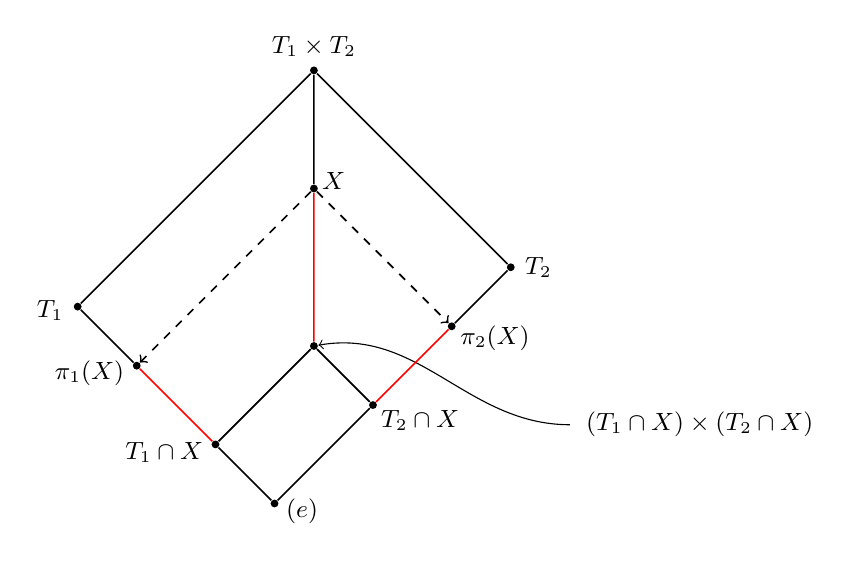
\begin{tikzpicture}[scale=.5]
    \node (e) at (0,0) [fill,circle,inner sep=1pt] {};
    \draw[font=\small] (.7,-.2) node {$(e)$};
    \node (T1capX) at (-1.5,1.5) [fill,circle,inner sep=1pt] {};
    \draw[font=\small] (-2.8,1.3) node {$T_1\cap X$};
    \node (T2capX) at (2.5,2.5) [fill,circle,inner sep=1pt] {};
    \draw[font=\small] (3.7,2.1) node {$T_2\cap X$};
    \node (pi1) at (-3.5,3.5) [fill,circle,inner sep=1pt] {};
    \draw[font=\small] (-4.7,3.3) node {$\pi_1(X)$};
    \node (pi2) at (4.5,4.5) [fill,circle,inner sep=1pt] {};
    \draw[font=\small] (5.6,4.2) node {$\pi_2(X)$};
    \node (Y) at (1,4) [fill,circle,inner sep=1pt] {};
    \draw[->] (7.5,2) to [out=180,in=10] (Y);
    \draw[font=\small] (10.8,2) node {$(T_1\cap X)\times (T_2 \cap X)$};

    \node (X) at (1,8) [fill,circle,inner sep=1pt] {};
    \draw[font=\small] (1.5,8.2) node {$X$};
    \node (T1) at (-5,5) [fill,circle,inner sep=1pt] {};
    \draw[font=\small] (-5.7,4.9) node {$T_1$};
    \node (T2) at (6,6) [fill,circle,inner sep=1pt] {};
    \draw[font=\small] (6.7,6) node {$T_2$};
    \node (T1T2) at (1,11) [fill,circle,inner sep=1pt] {};
    \draw[font=\small] (1,11.6) node {$T_1\times T_2$};


    \draw[semithick]
    (T1T2) to (X)
    (e) to (T1capX) to (Y) to (T2capX) to (e)
    (pi1) to (T1) to (T1T2) to (T2) to (pi2);

    \draw[->, dashed, semithick]
    (X) to (pi1);

    \draw[->, dashed, semithick]
    (X) to (pi2);
    
    \draw[red, semithick]
    (T1capX) to (pi1)
    (T2capX) to (pi2)
    (Y) to (X);
  \end{tikzpicture}
  \caption{Illustrates Theorem~\ref{thm:1} in case $n=2$.  Solid lines
    represent subgroup relations. Intervals colored red are isomorphic. Dashed
    lines emphasize the fact that the projections, $\pi_1(X)$ and
    $\pi_2(X)$, are not generally subgroups of $X$.}  
  \label{fig:theorem}
\end{center}
\end{figure}

Recall, $X$ is a subdirect product of $T_1, \dots, T_n$ provided
 $X \leq \prod\limits_k T_k $ and the projections are onto: $\pi_i(X)= T_i$.  We
denote this situation by  
%$X \stackrel{_{ \mathrm{sd}}}{\hookrightarrow} \prod_i T_i$.
$X \stackrel{_{\mathrm{sd}}}{\leq} \prod T_k$.
%$X \leq_{\mathrm{sd}}\prod_i T_i$.
The following is a consequence of Theorem~\ref{thm:1}:
% and the CFSG theorem:\footnote{The classification of
%finite simple groups (which is a theorem) is called ``the CFSG theorem.''}
\begin{corollary}
  If $T$ is a finite nonabelian simple group and 
$X \stackrel{_{\mathrm{sd}}}{\leq} T^n$,
%$X \stackrel{_{ \mathrm{sd}}}{\hookrightarrow} T^n$,
  then $T \cong X/ (T^{n-1}\cap X)$.  Thus, there are (at least) $n$ distinct normal
  subgroups of $X$ (namely,  $\hat{T}\cap X$) with the property that the
  quotient group is isomorphic to $T$.  In case $n=2$, every subdirect product
  of $T^2$ is isomorphic to $T$.
\end{corollary}


\subsection{Semidirect and Wreath Products}
This note describes some semidirect and wreath product constructions that I
recently learned about from some responses to my questions on MathOverflow.net.

John Shareshian responded to my question~\cite{MO63675} about which finite
groups contain $M_4$ as an upper interval, as follows.
If $H$ has trivial core in $G$ and $[H,G]\cong M_4$, then one of the following holds:
\begin{enumerate}
\item 
$G$ is the semidirect product $H(V+V)$, where $V$ is an irreducible
$F_3[H]$-module such that the only elements of $\GL(V)$ commuting with $H$ are
the scalar transformations 1 and -1. 

(This case occurs when every maximal subgroup containing $H$ has nontrivial core
in $G$. Your example $C_2:(C_3\times C_3)$ is of this type. This condition
should be sufficient and you can construct tons of examples of this type without
too much trouble.) 

\item $G$ is the semidirect product $MV$, where $V$ is an irreducible
  $F_3[M]$-module. There is a 1-dimensional subspace $W$ of $V$ such that
  $H=N_M(W)=C_M(W)$, and $C_V(H)=W$. In particular, no element of $M$ has $W$ as an
  eigenspace with eigenvalue -1. 

(This case occurs when some maximal $M$ containing $H$ has trivial core in $G$. Your
example $S_3$ is of this type. I don't know if there are lots of examples with $H$
maximal in $M$.) 
\end{enumerate}

In response to question~\cite{MO62495}, F.~Ladisch told me about the following
wreath product construction:
Let $H < G$ with $\Core_G(H) =  (e)$.  The $G$ acts faithfully on the cosets of
$H$, so identify $G$ with a transitive permutation group. Assume $G \leq
\Sym(\Gamma)$ is transitive, and suppose $X$ is a transitive permutation group
acting on the set $\Omega$. The \emph{wreath product}
of $G$ with $X$ is the semi-direct product 
\[
W=G^{\Omega} \rtimes X 
\]
Note that $G^{\Omega}$ is simply the set of maps $\{f:\Omega \rightarrow G\}$
with group multiplication given by the pointwise multiplication of the
coordinates 
\[
(f(\omega))_{\Omega} (h(\omega))_{\Omega} = (f(\omega) h(\omega))_{\Omega}  
\qquad (f, h \in G^\Omega).
\]
The group $X$ acts on the group $G^{\Omega}$ by the rule:
\[
f^x = (f(\omega^x))_{\Omega} \qquad (x\in X, f\in G^\Omega).
\]
so multiplication in the group $W$ is given by
\[
(f,x) (h,y) = fxhy = f h^x x y =(f h^x, x y) \qquad (x, y \in X, f, h\in G^\Omega).
\]
The group $W$ acts on the set $\Omega \times \Gamma$ by 
\[
(f,x) (\gamma, \omega) = \dots
\]
\[
(\omega, \gamma)(x,f) =  
(\omega x, \gamma((\omega x)f)), \quad \text{ where $f: \Omega \rightarrow G$
  and thus $(\omega x) f \in G$.}
\]
The stabilizer of $(\omega, \gamma)$ is then 
\[
W_{(\omega, \gamma)} = X_\omega \ltimes (G_\gamma \times G \times \cdots \times G)
\]
(where the component $G_\gamma$ occurs, strictly speaking, at position $\omega$). 
Now it is not difficult to see, that if a subgroup $K$ with 
$W(\omega, \gamma)\leq K$ contains an element $(x,f)$ with $x\notin X_\omega$,
then $K$ contains $G\times G\times \cdots \times G$. So either $K$ has the form
$Y\ltimes (G^\Omega)$ with $X_\omega < Y\leq X$, or it has the form
$X_\omega\ltimes (I\times G\times \cdots \times G)$ with $G_\gamma \leq I \leq G$.
So the interval $[W(\omega,\gamma),W]$ is lattice isomorphic to the lattice
obtained by putting $[X\omega,X]$ on top of $[G_\gamma,G]$. If the latter are
chains, then you get a chain, where the lengths add. Starting with a primitive
permutation group (non-solvable, if you wish) and repeating this contruction,
you get arbitrarily large chains. Even if you are interested in non-solvable
groups, I mention that the Sylow $p$-subgroup of $S_{p^n}$ is a special case of
this contruction.  


\newpage

\section{Congruence Lattices of Transitive G-sets}
In this note we list all congruence lattices of transitive G-sets in $\Eq(n)$
for $n=3,\dots, 15$ (with a few for $n=16$ as well).  This is possible because
of the following observation: If $G$ is an arbitrary transitive permutation
group of degree $n$ (the number of moved points), then the index of the
stabilizer $G_x$ is $[G: G_x] = n$, and the transitive G-set $\<X; G\> \cong 
\<G/G_x; G\>$ has $|X|=n$ and congruence lattice $\Con\<X; G\> \leq \Eq(n)$,
which is isomorphic to the interval $[G_x, G]$ in the subgroup lattice of $G$.  
Thus, sublattices of $\Eq(n)$ which are congruence lattices of transitive G-sets
are the intervals above stabilizer subgroups of transitive groups of degree $n$.
\\[8pt]
GAP has a library of transitive permutation groups of degree at most 30.
Therefore, for a transitive G-set $\<X; G\>$ with $|X|\leq 30$, the shape of $\Con\<X;
G\>$ can be computed with three simple GAP commands.  Take, for example,
$G=$ {\tt TransitiveGroup(4,2)} (the second transitive group of
degree 4).  The covering relations of the sublattice $\Con\<X; G\> \leq \Eq(4)$
are found by
{\small
\begin{verbatim}
gap> G := TransitiveGroup(4,2);     % returns E(4) = 2[x]2
gap> H := Stabilizer(G,1);          % returns Group(())
gap> intHG := IntermediateSubgroups(G,H);
rec( subgroups := [ Group([ (1,2)(3,4) ]), Group([ (1,4)(2,3) ]), Group([ (1,3)(2,4) ]) ], 
  inclusions := [ [ 0, 1 ], [ 0, 2 ], [ 0, 3 ], [ 1, 4 ], [ 2, 4 ], [ 3, 4 ] ] )
\end{verbatim}}
\noindent The list {\tt intHG.inclusions} (the last line above) shows that $\Con\<X; G\> \cong M_3$.
\\[6pt]
The following displays the number of transitive permutation groups of degree at
most 20: 
{\small
\begin{verbatim}
gap> List([1..20], x->NrTransitiveGroups(x));
[ 1, 1, 2, 5, 5, 16, 7, 50, 34, 45, 8, 301, 9, 63, 104, 1954, 10, 983, 8, 1117 ]
\end{verbatim}}
\noindent Many of these groups are \emph{primitive}, that is, the congruence
lattice of the associated G-set is just the two element lattice.  For example,
all transitive groups of prime degree are primitive.  So, in the list below, we
only present those G-set congruence lattices in $\Eq(n)$ for $n=4, 6, 8, 9,
10, 12, 14, 15$. 

Properties of transitive groups a given degree, $n$, can be checked with
the {\tt AllTransitiveGroups} function with {\tt NrMovedPoints} parameter set to
$n$.  For example, we can check for primitivity of transitive groups of degrees
5, 6, 7, and 11 as follows:
{\small
\begin{verbatim}
gap> List(AllTransitiveGroups(NrMovedPoints,5),IsPrimitive);
[ true, true, true, true, true ]
gap> List(AllTransitiveGroups(NrMovedPoints,6),IsPrimitive);
[ false, false, false, false, false, false, false, false, false, false, false, true,...
  ... false, true, true, true ]
gap> List(AllTransitiveGroups(NrMovedPoints,7),IsPrimitive);
[ true, true, true, true, true, true, true ]
gap> List(AllTransitiveGroups(NrMovedPoints,11),IsPrimitive);
[ true, true, true, true, true, true, true, true ]
\end{verbatim}}

%% \input{TransitiveGsetCongEx4.tex}
\begin{figure}[h]
\caption{Transitive G-set congruence lattices in Eq(4)}
\label{fig:4}
\begin{center}
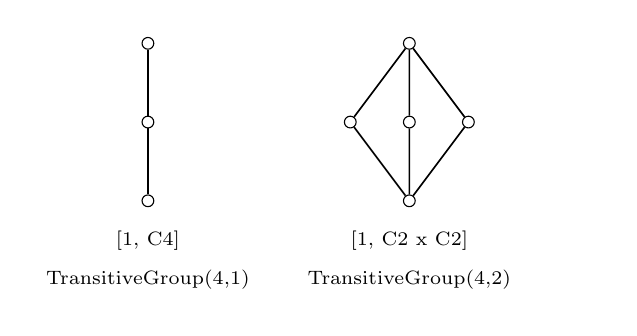
\begin{tikzpicture}[scale=.5]
\matrix[column sep=5mm,row sep=5mm]
{
\node (0) at (0,0) [draw, circle,inner sep=1.5pt] {};
\node (1) at (-0,1) [draw, circle, inner sep=1.5pt] {};
\node (2) at (-0,2) [draw, circle, inner sep=1.5pt] {};
\draw[font=\scriptsize] (0,-.5) node {[1, C4]};
\draw[font=\scriptsize] (0,-1) node {TransitiveGroup(4,1) };

\draw[semithick]
(0) to (1)
(1) to (2);
&
\node (0) at (0,0) [draw, circle,inner sep=1.5pt] {};
\node (1) at (-0,1) [draw, circle, inner sep=1.5pt] {};
\node (2) at (0.75,1) [draw, circle, inner sep=1.5pt] {};
\node (3) at (-0.75,1) [draw, circle, inner sep=1.5pt] {};
\node (4) at (-0,2) [draw, circle, inner sep=1.5pt] {};
\draw[font=\scriptsize] (0,-.5) node {[1, C2 x C2]};
\draw[font=\scriptsize] (0,-1) node {TransitiveGroup(4,2) };

\draw[semithick]
(0) to (1)
(0) to (2)
(0) to (3)
(1) to (4)
(2) to (4)
(3) to (4);
&
& \\
};
\end{tikzpicture}
\end{center}
\end{figure}



%% \input{TransitiveGsetCongEx6.tex}
\begin{figure}[h]
\caption{Transitive G-set congruence lattices in Eq(6)}
\label{fig:6}
\begin{center}
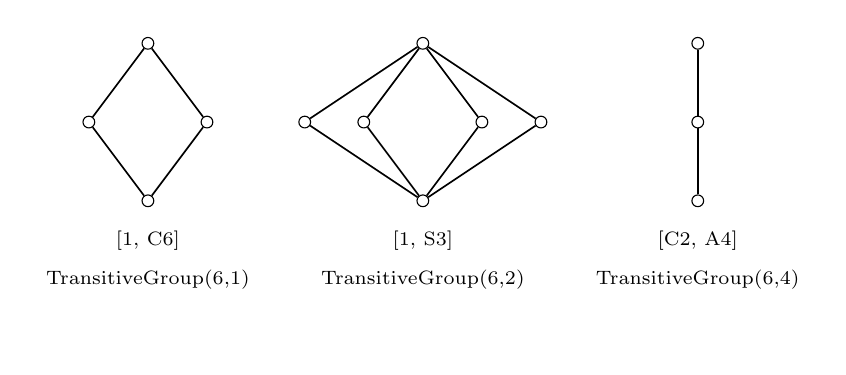
\begin{tikzpicture}[scale=.5]
\matrix[column sep=5mm,row sep=5mm]
{
\node (0) at (0,0) [draw, circle,inner sep=1.5pt] {};
\node (1) at (0.75,1) [draw, circle, inner sep=1.5pt] {};
\node (2) at (-0.75,1) [draw, circle, inner sep=1.5pt] {};
\node (3) at (-0,2) [draw, circle, inner sep=1.5pt] {};
\draw[font=\scriptsize] (0,-.5) node {[1, C6]};
\draw[font=\scriptsize] (0,-1) node {TransitiveGroup(6,1) };

\draw[semithick]
(0) to (1)
(0) to (2)
(1) to (3)
(2) to (3);
&
\node (0) at (0,0) [draw, circle,inner sep=1.5pt] {};
\node (1) at (0.75,1) [draw, circle, inner sep=1.5pt] {};
\node (2) at (-0.75,1) [draw, circle, inner sep=1.5pt] {};
\node (3) at (1.5,1) [draw, circle, inner sep=1.5pt] {};
\node (4) at (-1.5,1) [draw, circle, inner sep=1.5pt] {};
\node (5) at (-0,2) [draw, circle, inner sep=1.5pt] {};
\draw[font=\scriptsize] (0,-.5) node {[1, S3]};
\draw[font=\scriptsize] (0,-1) node {TransitiveGroup(6,2) };

\draw[semithick]
(0) to (1)
(0) to (2)
(0) to (3)
(0) to (4)
(1) to (5)
(2) to (5)
(3) to (5)
(4) to (5);
&
\node (0) at (0,0) [draw, circle,inner sep=1.5pt] {};
\node (1) at (-0,1) [draw, circle, inner sep=1.5pt] {};
\node (2) at (-0,2) [draw, circle, inner sep=1.5pt] {};
\draw[font=\scriptsize] (0,-.5) node {[C2, A4]};
\draw[font=\scriptsize] (0,-1) node {TransitiveGroup(6,4) };

\draw[semithick]
(0) to (1)
(1) to (2);
\\
\\
};
\end{tikzpicture}
\end{center}
\end{figure}

\newpage


%\input{TransitiveGsetCongEx8.tex}
\begin{figure}[h]
\caption{Transitive G-set congruence lattices in Eq(8)}
\label{fig:8}
\begin{center}
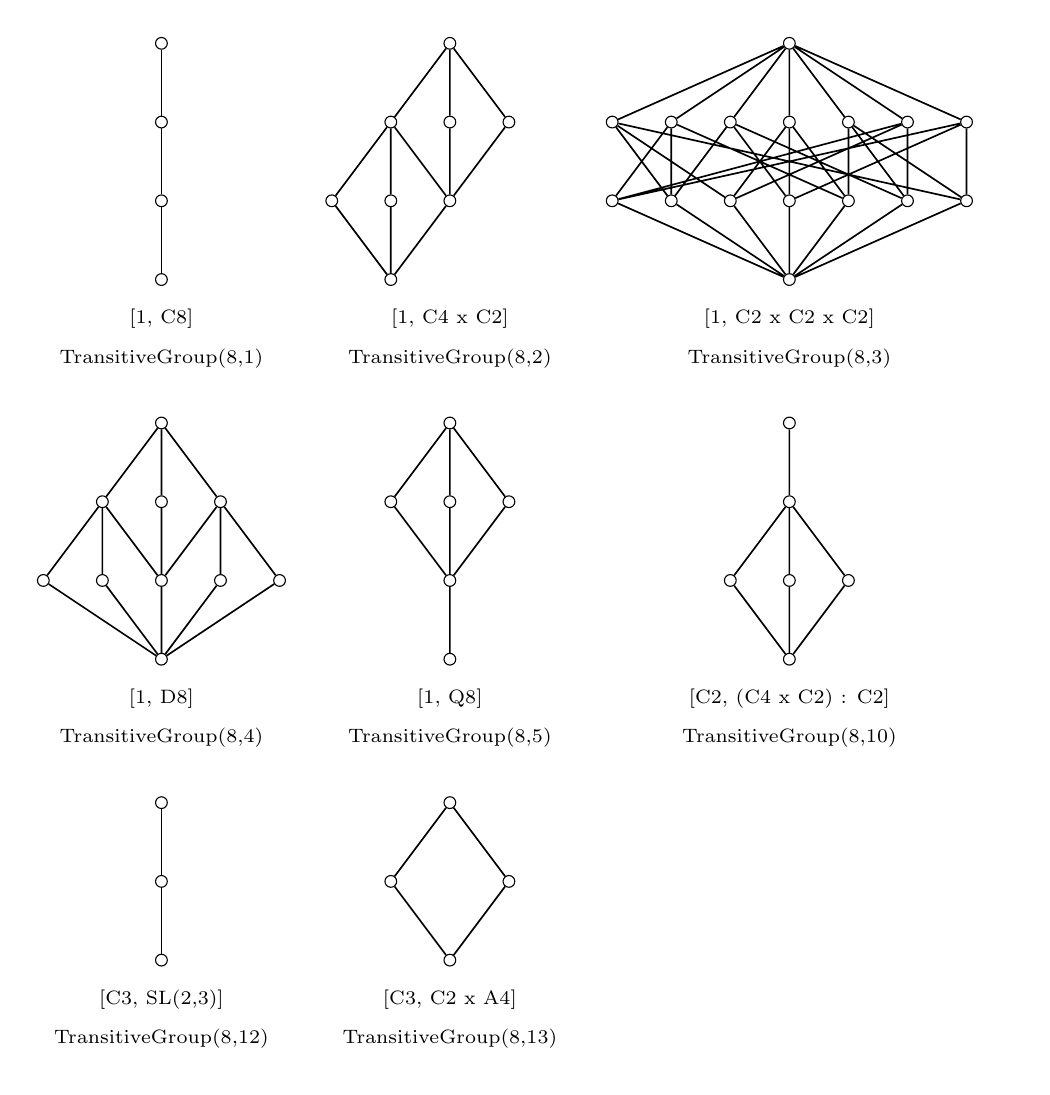
\begin{tikzpicture}[scale=.5]
\matrix[column sep=5mm,row sep=5mm]
{
\node (0) at (0,0) [draw, circle,inner sep=1.5pt] {};
\node (1) at (-0,1) [draw, circle, inner sep=1.5pt] {};
\node (2) at (-0,2) [draw, circle, inner sep=1.5pt] {};
\node (3) at (-0,3) [draw, circle, inner sep=1.5pt] {};
\draw[font=\scriptsize] (0,-.5) node {[1, C8]};
\draw[font=\scriptsize] (0,-1) node {TransitiveGroup(8,1) };

\draw[semithick]
(0) to (1)
(1) to (2)
(2) to (3);
&
%\node (0) at (0,0) [draw, circle,inner sep=1.5pt] {};
\node (0) at (-0.75,0) [draw, circle,inner sep=1.5pt] {};
\node (1) at (-0,1) [draw, circle, inner sep=1.5pt] {};
%\node (2) at (0.75,1) [draw, circle, inner sep=1.5pt] {};
\node (2) at (-1.5,1) [draw, circle, inner sep=1.5pt] {};
\node (3) at (-0.75,1) [draw, circle, inner sep=1.5pt] {};
%\node (4) at (-0,2) [draw, circle, inner sep=1.5pt] {};
\node (4) at (-0.75,2) [draw, circle, inner sep=1.5pt] {};
\node (5) at (0.75,2) [draw, circle, inner sep=1.5pt] {};
%\node (6) at (-0.75,2) [draw, circle, inner sep=1.5pt] {};
\node (6) at (0,2) [draw, circle, inner sep=1.5pt] {};
\node (7) at (-0,3) [draw, circle, inner sep=1.5pt] {};
\draw[font=\scriptsize] (0,-.5) node {[1, C4 x C2]};
\draw[font=\scriptsize] (0,-1) node {TransitiveGroup(8,2) };

\draw[semithick]
(0) to (1)
(0) to (2)
(0) to (3)
(1) to (4)
(1) to (5)
(1) to (6)
(2) to (4)
(3) to (4)
(4) to (7)
(5) to (7)
(6) to (7);
&
\node (0) at (0,0) [draw, circle,inner sep=1.5pt] {};
\node (1) at (-0,1) [draw, circle, inner sep=1.5pt] {};
\node (2) at (0.75,1) [draw, circle, inner sep=1.5pt] {};
\node (3) at (-0.75,1) [draw, circle, inner sep=1.5pt] {};
\node (4) at (1.5,1) [draw, circle, inner sep=1.5pt] {};
\node (5) at (-1.5,1) [draw, circle, inner sep=1.5pt] {};
\node (6) at (2.25,1) [draw, circle, inner sep=1.5pt] {};
\node (7) at (-2.25,1) [draw, circle, inner sep=1.5pt] {};
\node (8) at (-0,2) [draw, circle, inner sep=1.5pt] {};
\node (9) at (0.75,2) [draw, circle, inner sep=1.5pt] {};
\node (10) at (-0.75,2) [draw, circle, inner sep=1.5pt] {};
\node (11) at (1.5,2) [draw, circle, inner sep=1.5pt] {};
\node (12) at (-1.5,2) [draw, circle, inner sep=1.5pt] {};
\node (13) at (2.25,2) [draw, circle, inner sep=1.5pt] {};
\node (14) at (-2.25,2) [draw, circle, inner sep=1.5pt] {};
\node (15) at (-0,3) [draw, circle, inner sep=1.5pt] {};
\draw[font=\scriptsize] (0,-.5) node {[1, C2 x C2 x C2]};
\draw[font=\scriptsize] (0,-1) node {TransitiveGroup(8,3) };

\draw[semithick]
(0) to (1)
(0) to (2)
(0) to (3)
(0) to (4)
(0) to (5)
(0) to (6)
(0) to (7)
(1) to (8)
(1) to (10)
(1) to (13)
(2) to (8)
(2) to (9)
(2) to (12)
(3) to (8)
(3) to (11)
(3) to (14)
(4) to (9)
(4) to (10)
(4) to (11)
(5) to (10)
(5) to (12)
(5) to (14)
(6) to (9)
(6) to (13)
(6) to (14)
(7) to (11)
(7) to (12)
(7) to (13)
(8) to (15)
(9) to (15)
(10) to (15)
(11) to (15)
(12) to (15)
(13) to (15)
(14) to (15);
\\
\node (0) at (0,0) [draw, circle,inner sep=1.5pt] {};
\node (1) at (-0,1) [draw, circle, inner sep=1.5pt] {};
\node (2) at (0.75,1) [draw, circle, inner sep=1.5pt] {};
% \node (3) at (-0.75,1) [draw, circle, inner sep=1.5pt] {};
% \node (4) at (1.5,1) [draw, circle, inner sep=1.5pt] {};
\node (3) at (1.5,1) [draw, circle, inner sep=1.5pt] {};
\node (4) at (-0.75,1) [draw, circle, inner sep=1.5pt] {};
\node (5) at (-1.5,1) [draw, circle, inner sep=1.5pt] {};
% \node (6) at (-0,2) [draw, circle, inner sep=1.5pt] {};
% \node (7) at (0.75,2) [draw, circle, inner sep=1.5pt] {};
\node (6) at (0.75,2) [draw, circle, inner sep=1.5pt] {};
\node (7) at (0,2) [draw, circle, inner sep=1.5pt] {};
\node (8) at (-0.75,2) [draw, circle, inner sep=1.5pt] {};
\node (9) at (-0,3) [draw, circle, inner sep=1.5pt] {};
\draw[font=\scriptsize] (0,-.5) node {[1, D8]};
\draw[font=\scriptsize] (0,-1) node {TransitiveGroup(8,4) };

\draw[semithick]
(0) to (1)
(0) to (2)
(0) to (3)
(0) to (4)
(0) to (5)
(1) to (6)
(1) to (7)
(1) to (8)
(2) to (6)
(3) to (6)
(4) to (8)
(5) to (8)
(6) to (9)
(7) to (9)
(8) to (9);
&
\node (0) at (0,0) [draw, circle,inner sep=1.5pt] {};
\node (1) at (-0,1) [draw, circle, inner sep=1.5pt] {};
\node (2) at (-0,2) [draw, circle, inner sep=1.5pt] {};
\node (3) at (0.75,2) [draw, circle, inner sep=1.5pt] {};
\node (4) at (-0.75,2) [draw, circle, inner sep=1.5pt] {};
\node (5) at (-0,3) [draw, circle, inner sep=1.5pt] {};
\draw[font=\scriptsize] (0,-.5) node {[1, Q8]};
\draw[font=\scriptsize] (0,-1) node {TransitiveGroup(8,5) };

\draw[semithick]
(0) to (1)
(1) to (2)
(1) to (3)
(1) to (4)
(2) to (5)
(3) to (5)
(4) to (5);
&
\node (0) at (0,0) [draw, circle,inner sep=1.5pt] {};
\node (1) at (-0,1) [draw, circle, inner sep=1.5pt] {};
\node (2) at (0.75,1) [draw, circle, inner sep=1.5pt] {};
\node (3) at (-0.75,1) [draw, circle, inner sep=1.5pt] {};
\node (4) at (-0,2) [draw, circle, inner sep=1.5pt] {};
\node (5) at (-0,3) [draw, circle, inner sep=1.5pt] {};
\draw[font=\scriptsize] (0,-.5) node {[C2, (C4 x C2) : C2]};
\draw[font=\scriptsize] (0,-1) node {TransitiveGroup(8,10) };

\draw[semithick]
(0) to (1)
(0) to (2)
(0) to (3)
(1) to (4)
(2) to (4)
(3) to (4)
(4) to (5);
\\
\node (0) at (0,0) [draw, circle,inner sep=1.5pt] {};
\node (1) at (-0,1) [draw, circle, inner sep=1.5pt] {};
\node (2) at (-0,2) [draw, circle, inner sep=1.5pt] {};
\draw[font=\scriptsize] (0,-.5) node {[C3, SL(2,3)]};
\draw[font=\scriptsize] (0,-1) node {TransitiveGroup(8,12) };

\draw[semithick]
(0) to (1)
(1) to (2);
&
\node (0) at (0,0) [draw, circle,inner sep=1.5pt] {};
\node (1) at (0.75,1) [draw, circle, inner sep=1.5pt] {};
\node (2) at (-0.75,1) [draw, circle, inner sep=1.5pt] {};
\node (3) at (-0,2) [draw, circle, inner sep=1.5pt] {};
\draw[font=\scriptsize] (0,-.5) node {[C3, C2 x A4]};
\draw[font=\scriptsize] (0,-1) node {TransitiveGroup(8,13) };

\draw[semithick]
(0) to (1)
(0) to (2)
(1) to (3)
(2) to (3);
&
& \\
};
\end{tikzpicture}
\end{center}
\end{figure}

\newpage

%% \input{TransitiveGsetCongEx9.tex}
\begin{figure}[h]
\caption{Transitive G-set congruence lattices in Eq(9)}
\label{fig:9}
\begin{center}
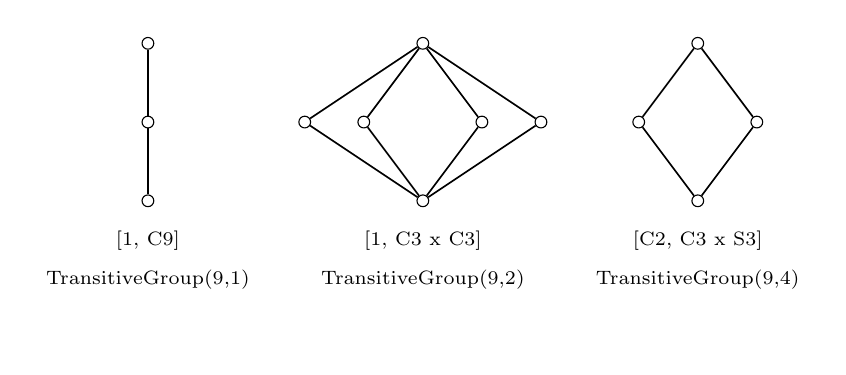
\begin{tikzpicture}[scale=.5]
\matrix[column sep=5mm,row sep=5mm]
{
\node (0) at (0,0) [draw, circle,inner sep=1.5pt] {};
\node (1) at (-0,1) [draw, circle, inner sep=1.5pt] {};
\node (2) at (-0,2) [draw, circle, inner sep=1.5pt] {};
\draw[font=\scriptsize] (0,-.5) node {[1, C9]};
\draw[font=\scriptsize] (0,-1) node {TransitiveGroup(9,1) };

\draw[semithick]
(0) to (1)
(1) to (2);
&
\node (0) at (0,0) [draw, circle,inner sep=1.5pt] {};
\node (1) at (0.75,1) [draw, circle, inner sep=1.5pt] {};
\node (2) at (-0.75,1) [draw, circle, inner sep=1.5pt] {};
\node (3) at (1.5,1) [draw, circle, inner sep=1.5pt] {};
\node (4) at (-1.5,1) [draw, circle, inner sep=1.5pt] {};
\node (5) at (-0,2) [draw, circle, inner sep=1.5pt] {};
\draw[font=\scriptsize] (0,-.5) node {[1, C3 x C3]};
\draw[font=\scriptsize] (0,-1) node {TransitiveGroup(9,2) };

\draw[semithick]
(0) to (1)
(0) to (2)
(0) to (3)
(0) to (4)
(1) to (5)
(2) to (5)
(3) to (5)
(4) to (5);
&
\node (0) at (0,0) [draw, circle,inner sep=1.5pt] {};
\node (1) at (0.75,1) [draw, circle, inner sep=1.5pt] {};
\node (2) at (-0.75,1) [draw, circle, inner sep=1.5pt] {};
\node (3) at (-0,2) [draw, circle, inner sep=1.5pt] {};
\draw[font=\scriptsize] (0,-.5) node {[C2, C3 x S3]};
\draw[font=\scriptsize] (0,-1) node {TransitiveGroup(9,4) };

\draw[semithick]
(0) to (1)
(0) to (2)
(1) to (3)
(2) to (3);
\\
\\
};
\end{tikzpicture}
\end{center}
\end{figure}

\newpage





%% \input{TransitiveGsetCongEx10.tex}
\begin{figure}[h]
\caption{Transitive G-set congruence lattices in Eq(10)}
\label{fig:10}
\begin{center}
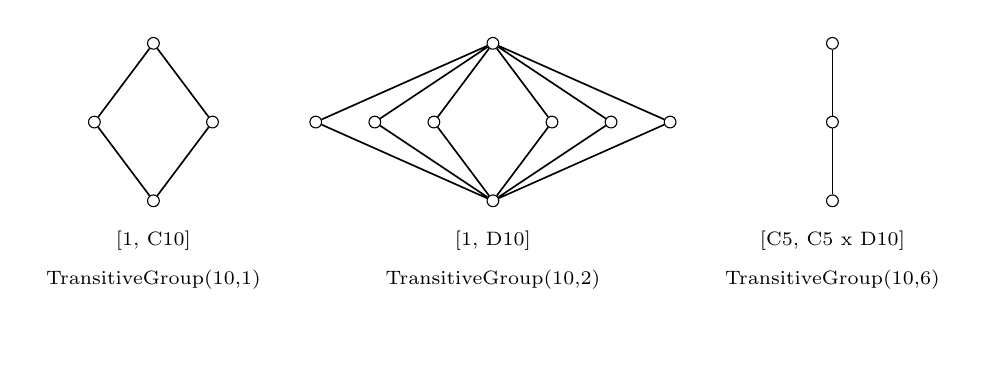
\begin{tikzpicture}[scale=.5]
\matrix[column sep=5mm,row sep=5mm]
{
\node (0) at (0,0) [draw, circle,inner sep=1.5pt] {};
\node (1) at (0.75,1) [draw, circle, inner sep=1.5pt] {};
\node (2) at (-0.75,1) [draw, circle, inner sep=1.5pt] {};
\node (3) at (-0,2) [draw, circle, inner sep=1.5pt] {};
\draw[font=\scriptsize] (0,-.5) node {[1, C10]};
\draw[font=\scriptsize] (0,-1) node {TransitiveGroup(10,1) };

\draw[semithick]
(0) to (1)
(0) to (2)
(1) to (3)
(2) to (3);
&
\node (0) at (0,0) [draw, circle,inner sep=1.5pt] {};
\node (1) at (0.75,1) [draw, circle, inner sep=1.5pt] {};
\node (2) at (-0.75,1) [draw, circle, inner sep=1.5pt] {};
\node (3) at (1.5,1) [draw, circle, inner sep=1.5pt] {};
\node (4) at (-1.5,1) [draw, circle, inner sep=1.5pt] {};
\node (5) at (2.25,1) [draw, circle, inner sep=1.5pt] {};
\node (6) at (-2.25,1) [draw, circle, inner sep=1.5pt] {};
\node (7) at (-0,2) [draw, circle, inner sep=1.5pt] {};
\draw[font=\scriptsize] (0,-.5) node {[1, D10]};
\draw[font=\scriptsize] (0,-1) node {TransitiveGroup(10,2) };

\draw[semithick]
(0) to (1)
(0) to (2)
(0) to (3)
(0) to (4)
(0) to (5)
(0) to (6)
(1) to (7)
(2) to (7)
(3) to (7)
(4) to (7)
(5) to (7)
(6) to (7);
&
\node (0) at (0,0) [draw, circle,inner sep=1.5pt] {};
\node (1) at (-0,1) [draw, circle, inner sep=1.5pt] {};
\node (2) at (-0,2) [draw, circle, inner sep=1.5pt] {};
\draw[font=\scriptsize] (0,-.5) node {[C5, C5 x D10]};
\draw[font=\scriptsize] (0,-1) node {TransitiveGroup(10,6) };

\draw[semithick]
(0) to (1)
(1) to (2);
\\
\\
};
\end{tikzpicture}
\end{center}
\end{figure}

\newpage


%% \input{TransitiveGsetCongEx12.tex}
\begin{figure}[h]
\caption{Transitive G-set congruence lattices in Eq(12)}
\label{fig:12}
\begin{center}
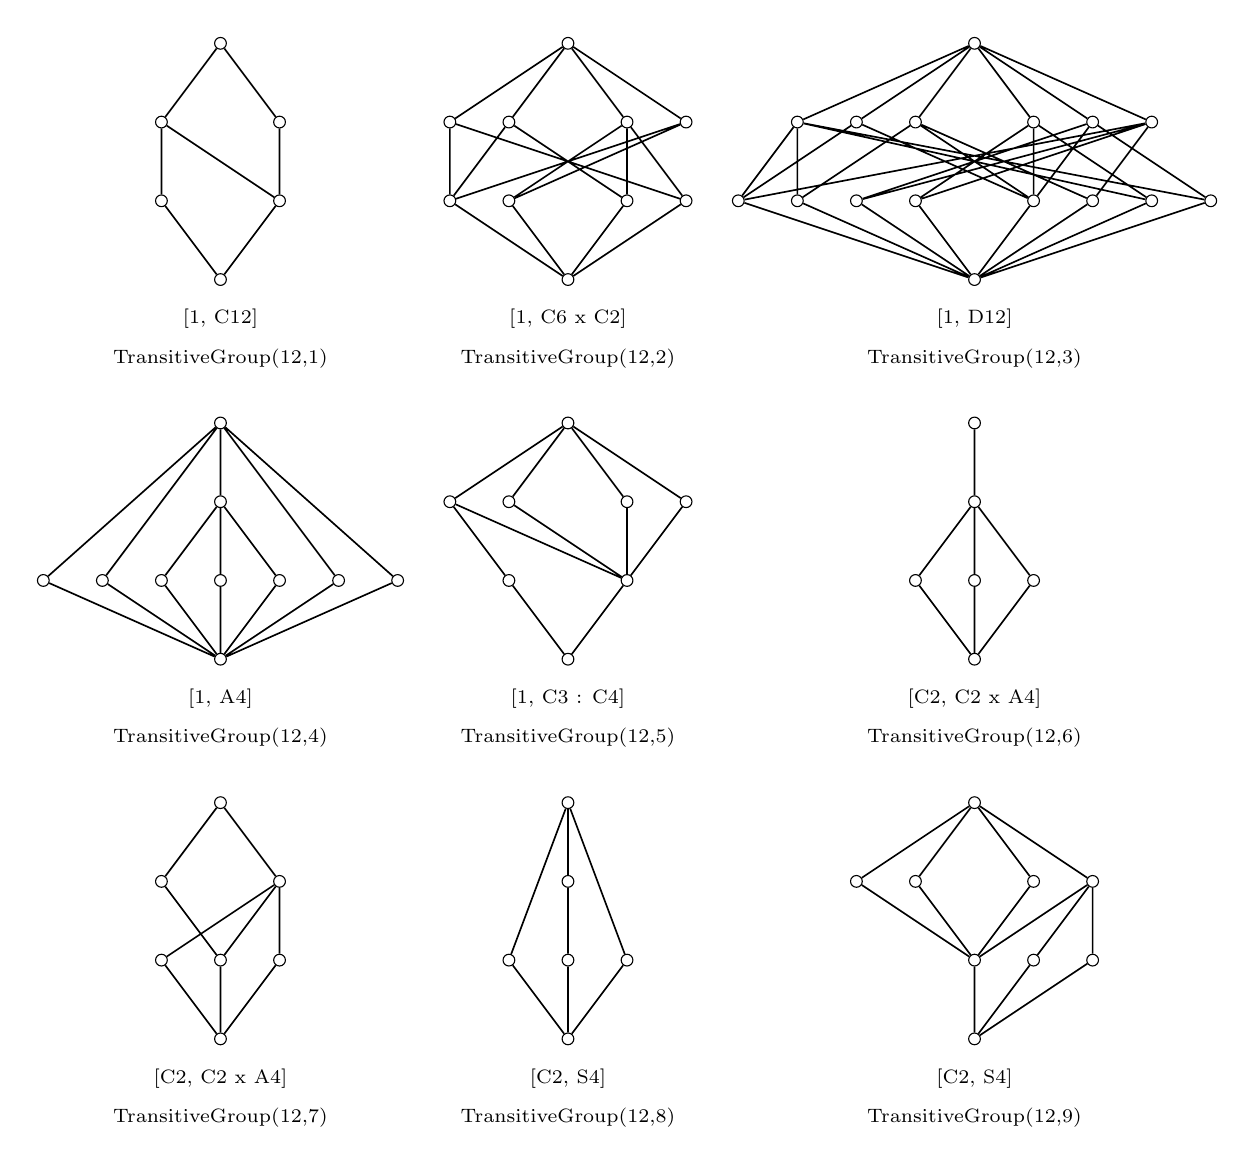
\begin{tikzpicture}[scale=.5]
\matrix[column sep=5mm,row sep=5mm]
{
\node (0) at (0,0) [draw, circle,inner sep=1.5pt] {};
\node (1) at (0.75,1) [draw, circle, inner sep=1.5pt] {};
\node (2) at (-0.75,1) [draw, circle, inner sep=1.5pt] {};
\node (3) at (0.75,2) [draw, circle, inner sep=1.5pt] {};
\node (4) at (-0.75,2) [draw, circle, inner sep=1.5pt] {};
\node (5) at (-0,3) [draw, circle, inner sep=1.5pt] {};
\draw[font=\scriptsize] (0,-.5) node {[1, C12]};
\draw[font=\scriptsize] (0,-1) node {TransitiveGroup(12,1) };

\draw[semithick]
(0) to (1)
(0) to (2)
(1) to (3)
(1) to (4)
(2) to (4)
(3) to (5)
(4) to (5);
&
\node (0) at (0,0) [draw, circle,inner sep=1.5pt] {};
\node (1) at (0.75,1) [draw, circle, inner sep=1.5pt] {};
\node (2) at (-0.75,1) [draw, circle, inner sep=1.5pt] {};
\node (3) at (1.5,1) [draw, circle, inner sep=1.5pt] {};
\node (4) at (-1.5,1) [draw, circle, inner sep=1.5pt] {};
\node (5) at (0.75,2) [draw, circle, inner sep=1.5pt] {};
\node (6) at (-0.75,2) [draw, circle, inner sep=1.5pt] {};
\node (7) at (1.5,2) [draw, circle, inner sep=1.5pt] {};
\node (8) at (-1.5,2) [draw, circle, inner sep=1.5pt] {};
\node (9) at (-0,3) [draw, circle, inner sep=1.5pt] {};
\draw[font=\scriptsize] (0,-.5) node {[1, C6 x C2]};
\draw[font=\scriptsize] (0,-1) node {TransitiveGroup(12,2) };

\draw[semithick]
(0) to (1)
(0) to (2)
(0) to (3)
(0) to (4)
(1) to (5)
(1) to (6)
(2) to (5)
(2) to (7)
(3) to (5)
(3) to (8)
(4) to (6)
(4) to (7)
(4) to (8)
(5) to (9)
(6) to (9)
(7) to (9)
(8) to (9);
&
\node (0) at (0,0) [draw, circle,inner sep=1.5pt] {};
\node (1) at (0.75,1) [draw, circle, inner sep=1.5pt] {};
\node (2) at (-0.75,1) [draw, circle, inner sep=1.5pt] {};
\node (3) at (1.5,1) [draw, circle, inner sep=1.5pt] {};
\node (4) at (-1.5,1) [draw, circle, inner sep=1.5pt] {};
\node (5) at (2.25,1) [draw, circle, inner sep=1.5pt] {};
\node (6) at (-2.25,1) [draw, circle, inner sep=1.5pt] {};
\node (7) at (3,1) [draw, circle, inner sep=1.5pt] {};
\node (8) at (-3,1) [draw, circle, inner sep=1.5pt] {};
\node (9) at (0.75,2) [draw, circle, inner sep=1.5pt] {};
\node (10) at (-0.75,2) [draw, circle, inner sep=1.5pt] {};
\node (11) at (1.5,2) [draw, circle, inner sep=1.5pt] {};
\node (12) at (-1.5,2) [draw, circle, inner sep=1.5pt] {};
\node (13) at (2.25,2) [draw, circle, inner sep=1.5pt] {};
\node (14) at (-2.25,2) [draw, circle, inner sep=1.5pt] {};
\node (15) at (-0,3) [draw, circle, inner sep=1.5pt] {};
\draw[font=\scriptsize] (0,-.5) node {[1, D12]};
\draw[font=\scriptsize] (0,-1) node {TransitiveGroup(12,3) };

\draw[semithick]
(0) to (1)
(0) to (2)
(0) to (3)
(0) to (4)
(0) to (5)
(0) to (6)
(0) to (7)
(0) to (8)
(1) to (9)
(1) to (10)
(1) to (11)
(1) to (12)
(2) to (9)
(2) to (13)
(3) to (10)
(3) to (13)
(4) to (11)
(4) to (13)
(5) to (9)
(5) to (14)
(6) to (10)
(6) to (14)
(7) to (11)
(7) to (14)
(8) to (12)
(8) to (13)
(8) to (14)
(9) to (15)
(10) to (15)
(11) to (15)
(12) to (15)
(13) to (15)
(14) to (15);
\\
\node (0) at (0,0) [draw, circle,inner sep=1.5pt] {};
\node (1) at (-0,1) [draw, circle, inner sep=1.5pt] {};
\node (2) at (0.75,1) [draw, circle, inner sep=1.5pt] {};
\node (3) at (-0.75,1) [draw, circle, inner sep=1.5pt] {};
\node (4) at (1.5,1) [draw, circle, inner sep=1.5pt] {};
\node (5) at (-1.5,1) [draw, circle, inner sep=1.5pt] {};
\node (6) at (2.25,1) [draw, circle, inner sep=1.5pt] {};
\node (7) at (-2.25,1) [draw, circle, inner sep=1.5pt] {};
\node (8) at (-0,2) [draw, circle, inner sep=1.5pt] {};
\node (9) at (-0,3) [draw, circle, inner sep=1.5pt] {};
\draw[font=\scriptsize] (0,-.5) node {[1, A4]};
\draw[font=\scriptsize] (0,-1) node {TransitiveGroup(12,4) };

\draw[semithick]
(0) to (1)
(0) to (2)
(0) to (3)
(0) to (4)
(0) to (5)
(0) to (6)
(0) to (7)
(1) to (8)
(2) to (8)
(3) to (8)
(4) to (9)
(5) to (9)
(6) to (9)
(7) to (9)
(8) to (9);
&
\node (0) at (0,0) [draw, circle,inner sep=1.5pt] {};
\node (1) at (0.75,1) [draw, circle, inner sep=1.5pt] {};
\node (2) at (-0.75,1) [draw, circle, inner sep=1.5pt] {};
\node (3) at (0.75,2) [draw, circle, inner sep=1.5pt] {};
\node (4) at (-0.75,2) [draw, circle, inner sep=1.5pt] {};
\node (5) at (1.5,2) [draw, circle, inner sep=1.5pt] {};
\node (6) at (-1.5,2) [draw, circle, inner sep=1.5pt] {};
\node (7) at (-0,3) [draw, circle, inner sep=1.5pt] {};
\draw[font=\scriptsize] (0,-.5) node {[1, C3 : C4]};
\draw[font=\scriptsize] (0,-1) node {TransitiveGroup(12,5) };

\draw[semithick]
(0) to (1)
(0) to (2)
(1) to (3)
(1) to (4)
(1) to (5)
(1) to (6)
(2) to (6)
(3) to (7)
(4) to (7)
(5) to (7)
(6) to (7);
&
\node (0) at (0,0) [draw, circle,inner sep=1.5pt] {};
\node (1) at (-0,1) [draw, circle, inner sep=1.5pt] {};
\node (2) at (0.75,1) [draw, circle, inner sep=1.5pt] {};
\node (3) at (-0.75,1) [draw, circle, inner sep=1.5pt] {};
\node (4) at (-0,2) [draw, circle, inner sep=1.5pt] {};
\node (5) at (-0,3) [draw, circle, inner sep=1.5pt] {};
\draw[font=\scriptsize] (0,-.5) node {[C2, C2 x A4]};
\draw[font=\scriptsize] (0,-1) node {TransitiveGroup(12,6) };

\draw[semithick]
(0) to (1)
(0) to (2)
(0) to (3)
(1) to (4)
(2) to (4)
(3) to (4)
(4) to (5);
\\
\node (0) at (0,0) [draw, circle,inner sep=1.5pt] {};
\node (1) at (-0,1) [draw, circle, inner sep=1.5pt] {};
\node (2) at (0.75,1) [draw, circle, inner sep=1.5pt] {};
\node (3) at (-0.75,1) [draw, circle, inner sep=1.5pt] {};
\node (4) at (0.75,2) [draw, circle, inner sep=1.5pt] {};
\node (5) at (-0.75,2) [draw, circle, inner sep=1.5pt] {};
\node (6) at (-0,3) [draw, circle, inner sep=1.5pt] {};
\draw[font=\scriptsize] (0,-.5) node {[C2, C2 x A4]};
\draw[font=\scriptsize] (0,-1) node {TransitiveGroup(12,7) };

\draw[semithick]
(0) to (1)
(0) to (2)
(0) to (3)
(1) to (4)
(1) to (5)
(2) to (4)
(3) to (4)
(4) to (6)
(5) to (6);
&
\node (0) at (0,0) [draw, circle,inner sep=1.5pt] {};
\node (1) at (-0,1) [draw, circle, inner sep=1.5pt] {};
\node (2) at (0.75,1) [draw, circle, inner sep=1.5pt] {};
\node (3) at (-0.75,1) [draw, circle, inner sep=1.5pt] {};
\node (4) at (-0,2) [draw, circle, inner sep=1.5pt] {};
\node (5) at (-0,3) [draw, circle, inner sep=1.5pt] {};
\draw[font=\scriptsize] (0,-.5) node {[C2, S4]};
\draw[font=\scriptsize] (0,-1) node {TransitiveGroup(12,8) };

\draw[semithick]
(0) to (1)
(0) to (2)
(0) to (3)
(1) to (4)
(2) to (5)
(3) to (5)
(4) to (5);
&
 \node (0) at (0,0) [draw, circle,inner sep=1.5pt] {};
% \node (1) at (-0,1) [draw, circle, inner sep=1.5pt] {};
% \node (2) at (0.75,1) [draw, circle, inner sep=1.5pt] {};
% \node (3) at (-0.75,1) [draw, circle, inner sep=1.5pt] {};
%\node (0) at (0.75,0) [draw, circle,inner sep=1.5pt] {};
\node (1) at (0.75,1) [draw, circle, inner sep=1.5pt] {};
\node (2) at (1.5,1) [draw, circle, inner sep=1.5pt] {};
\node (3) at (0,1) [draw, circle, inner sep=1.5pt] {};
\node (4) at (0.75,2) [draw, circle, inner sep=1.5pt] {};
\node (5) at (-0.75,2) [draw, circle, inner sep=1.5pt] {};
\node (6) at (1.5,2) [draw, circle, inner sep=1.5pt] {};
\node (7) at (-1.5,2) [draw, circle, inner sep=1.5pt] {};
\node (8) at (-0,3) [draw, circle, inner sep=1.5pt] {};
\draw[font=\scriptsize] (0,-.5) node {[C2, S4]};
\draw[font=\scriptsize] (0,-1) node {TransitiveGroup(12,9) };

\draw[semithick]
(0) to (1)
(0) to (2)
(0) to (3)
(1) to (6)
(2) to (6)
(3) to (4)
(3) to (5)
(3) to (6)
(3) to (7)
(4) to (8)
(5) to (8)
(6) to (8)
(7) to (8);
\\
};
\end{tikzpicture}
\end{center}
\end{figure}

\newpage

\begin{figure}[h]
\caption{Transitive G-set congruence lattices in Eq(12) (continued)}
\label{fig:12b}
\begin{center}
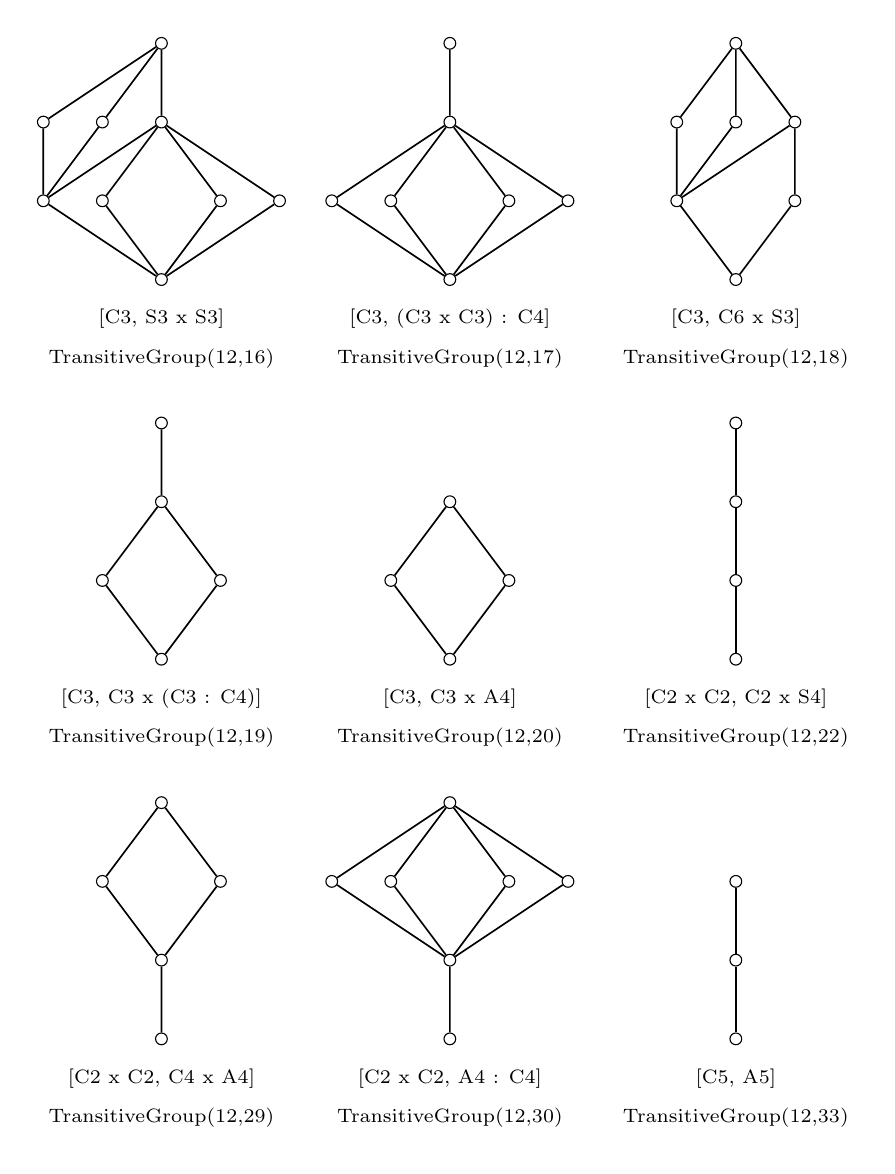
\begin{tikzpicture}[scale=.5]
\matrix[column sep=5mm,row sep=5mm]
{
\node (0) at (0,0) [draw, circle,inner sep=1.5pt] {};
\node (1) at (0.75,1) [draw, circle, inner sep=1.5pt] {};
\node (2) at (-0.75,1) [draw, circle, inner sep=1.5pt] {};
\node (3) at (1.5,1) [draw, circle, inner sep=1.5pt] {};
\node (4) at (-1.5,1) [draw, circle, inner sep=1.5pt] {};
% \node (5) at (-0,2) [draw, circle, inner sep=1.5pt] {};
% \node (6) at (0.75,2) [draw, circle, inner sep=1.5pt] {};
% \node (7) at (-0.75,2) [draw, circle, inner sep=1.5pt] {};
\node (5) at (-0.75,2) [draw, circle, inner sep=1.5pt] {};
\node (6) at (-1.5,2) [draw, circle, inner sep=1.5pt] {};
\node (7) at (0,2) [draw, circle, inner sep=1.5pt] {};
\node (8) at (-0,3) [draw, circle, inner sep=1.5pt] {};
\draw[font=\scriptsize] (0,-.5) node {[C3, S3 x S3]};
\draw[font=\scriptsize] (0,-1) node {TransitiveGroup(12,16) };

\draw[semithick]
(0) to (1)
(0) to (2)
(0) to (3)
(0) to (4)
(1) to (7)
(2) to (7)
(3) to (7)
(4) to (5)
(4) to (6)
(4) to (7)
(5) to (8)
(6) to (8)
(7) to (8);
&
\node (0) at (0,0) [draw, circle,inner sep=1.5pt] {};
\node (1) at (0.75,1) [draw, circle, inner sep=1.5pt] {};
\node (2) at (-0.75,1) [draw, circle, inner sep=1.5pt] {};
\node (3) at (1.5,1) [draw, circle, inner sep=1.5pt] {};
\node (4) at (-1.5,1) [draw, circle, inner sep=1.5pt] {};
\node (5) at (-0,2) [draw, circle, inner sep=1.5pt] {};
\node (6) at (-0,3) [draw, circle, inner sep=1.5pt] {};
\draw[font=\scriptsize] (0,-.5) node {[C3, (C3 x C3) : C4]};
\draw[font=\scriptsize] (0,-1) node {TransitiveGroup(12,17) };

\draw[semithick]
(0) to (1)
(0) to (2)
(0) to (3)
(0) to (4)
(1) to (5)
(2) to (5)
(3) to (5)
(4) to (5)
(5) to (6);
&
\node (0) at (0,0) [draw, circle,inner sep=1.5pt] {};
\node (1) at (0.75,1) [draw, circle, inner sep=1.5pt] {};
\node (2) at (-0.75,1) [draw, circle, inner sep=1.5pt] {};
\node (3) at (-0,2) [draw, circle, inner sep=1.5pt] {};
\node (4) at (0.75,2) [draw, circle, inner sep=1.5pt] {};
\node (5) at (-0.75,2) [draw, circle, inner sep=1.5pt] {};
\node (6) at (-0,3) [draw, circle, inner sep=1.5pt] {};
\draw[font=\scriptsize] (0,-.5) node {[C3, C6 x S3]};
\draw[font=\scriptsize] (0,-1) node {TransitiveGroup(12,18) };

\draw[semithick]
(0) to (1)
(0) to (2)
(1) to (4)
(2) to (3)
(2) to (4)
(2) to (5)
(3) to (6)
(4) to (6)
(5) to (6);
\\
\node (0) at (0,0) [draw, circle,inner sep=1.5pt] {};
\node (1) at (0.75,1) [draw, circle, inner sep=1.5pt] {};
\node (2) at (-0.75,1) [draw, circle, inner sep=1.5pt] {};
\node (3) at (-0,2) [draw, circle, inner sep=1.5pt] {};
\node (4) at (-0,3) [draw, circle, inner sep=1.5pt] {};
\draw[font=\scriptsize] (0,-.5) node {[C3, C3 x (C3 : C4)]};
\draw[font=\scriptsize] (0,-1) node {TransitiveGroup(12,19) };

\draw[semithick]
(0) to (1)
(0) to (2)
(1) to (3)
(2) to (3)
(3) to (4);
&
\node (0) at (0,0) [draw, circle,inner sep=1.5pt] {};
\node (1) at (0.75,1) [draw, circle, inner sep=1.5pt] {};
\node (2) at (-0.75,1) [draw, circle, inner sep=1.5pt] {};
\node (3) at (-0,2) [draw, circle, inner sep=1.5pt] {};
\draw[font=\scriptsize] (0,-.5) node {[C3, C3 x A4]};
\draw[font=\scriptsize] (0,-1) node {TransitiveGroup(12,20) };

\draw[semithick]
(0) to (1)
(0) to (2)
(1) to (3)
(2) to (3);
&
\node (0) at (0,0) [draw, circle,inner sep=1.5pt] {};
\node (1) at (-0,1) [draw, circle, inner sep=1.5pt] {};
\node (2) at (-0,2) [draw, circle, inner sep=1.5pt] {};
\node (3) at (-0,3) [draw, circle, inner sep=1.5pt] {};
\draw[font=\scriptsize] (0,-.5) node {[C2 x C2, C2 x S4]};
\draw[font=\scriptsize] (0,-1) node {TransitiveGroup(12,22) };

\draw[semithick]
(0) to (1)
(1) to (2)
(2) to (3);
\\
\node (0) at (0,0) [draw, circle,inner sep=1.5pt] {};
\node (1) at (-0,1) [draw, circle, inner sep=1.5pt] {};
\node (2) at (0.75,2) [draw, circle, inner sep=1.5pt] {};
\node (3) at (-0.75,2) [draw, circle, inner sep=1.5pt] {};
\node (4) at (-0,3) [draw, circle, inner sep=1.5pt] {};
\draw[font=\scriptsize] (0,-.5) node {[C2 x C2, C4 x A4]};
\draw[font=\scriptsize] (0,-1) node {TransitiveGroup(12,29) };

\draw[semithick]
(0) to (1)
(1) to (2)
(1) to (3)
(2) to (4)
(3) to (4);
&
\node (0) at (0,0) [draw, circle,inner sep=1.5pt] {};
\node (1) at (-0,1) [draw, circle, inner sep=1.5pt] {};
\node (2) at (0.75,2) [draw, circle, inner sep=1.5pt] {};
\node (3) at (-0.75,2) [draw, circle, inner sep=1.5pt] {};
\node (4) at (1.5,2) [draw, circle, inner sep=1.5pt] {};
\node (5) at (-1.5,2) [draw, circle, inner sep=1.5pt] {};
\node (6) at (-0,3) [draw, circle, inner sep=1.5pt] {};
\draw[font=\scriptsize] (0,-.5) node {[C2 x C2, A4 : C4]};
\draw[font=\scriptsize] (0,-1) node {TransitiveGroup(12,30) };

\draw[semithick]
(0) to (1)
(1) to (2)
(1) to (3)
(1) to (4)
(1) to (5)
(2) to (6)
(3) to (6)
(4) to (6)
(5) to (6);
&
\node (0) at (0,0) [draw, circle,inner sep=1.5pt] {};
\node (1) at (-0,1) [draw, circle, inner sep=1.5pt] {};
\node (2) at (-0,2) [draw, circle, inner sep=1.5pt] {};
\draw[font=\scriptsize] (0,-.5) node {[C5, A5]};
\draw[font=\scriptsize] (0,-1) node {TransitiveGroup(12,33) };

\draw[semithick]
(0) to (1)
(1) to (2);
\\
};
\end{tikzpicture}
\end{center}
\end{figure}

\newpage

\begin{figure}[h]
\caption{Transitive G-set congruence lattices in Eq(12) (continued)}
\label{fig:12c}
\begin{center}
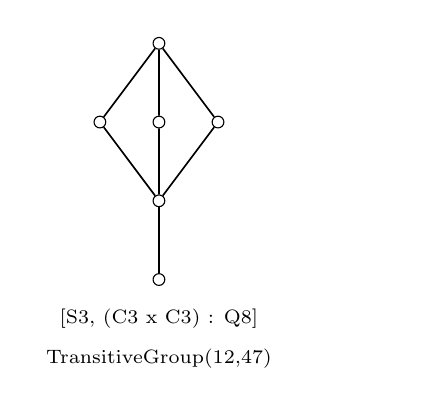
\begin{tikzpicture}[scale=.5]
\matrix[column sep=5mm,row sep=5mm]
{
\node (0) at (0,0) [draw, circle,inner sep=1.5pt] {};
\node (1) at (-0,1) [draw, circle, inner sep=1.5pt] {};
\node (2) at (-0,2) [draw, circle, inner sep=1.5pt] {};
\node (3) at (0.75,2) [draw, circle, inner sep=1.5pt] {};
\node (4) at (-0.75,2) [draw, circle, inner sep=1.5pt] {};
\node (5) at (-0,3) [draw, circle, inner sep=1.5pt] {};
\draw[font=\scriptsize] (0,-.5) node {[S3, (C3 x C3) : Q8]};
\draw[font=\scriptsize] (0,-1) node {TransitiveGroup(12,47) };

\draw[semithick]
(0) to (1)
(1) to (2)
(1) to (3)
(1) to (4)
(2) to (5)
(3) to (5)
(4) to (5);
&
& & \\
};
\end{tikzpicture}
\end{center}
\end{figure}

\newpage


%% \input{TransitiveGsetCongEx14.tex}
\begin{figure}[h]
\caption{Transitive G-set congruence lattices in Eq(14)}
\label{fig:14}
\begin{center}
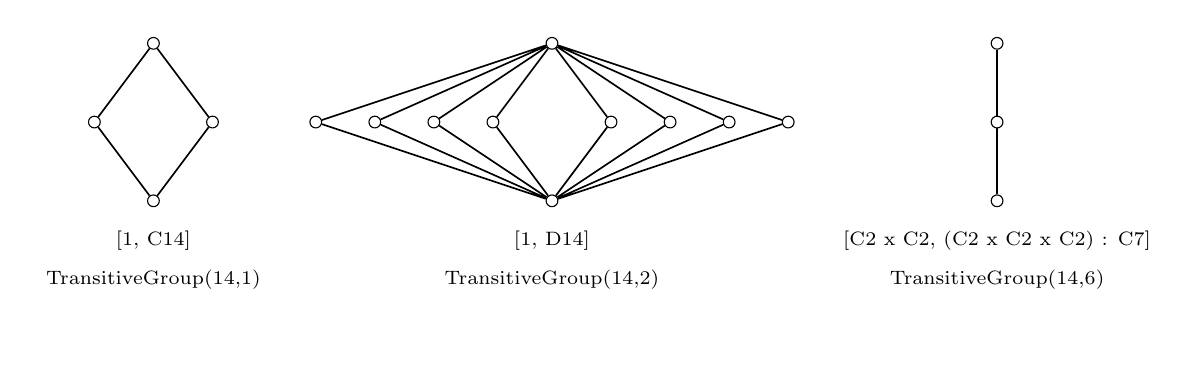
\begin{tikzpicture}[scale=.5]
\matrix[column sep=5mm,row sep=5mm]
{
\node (0) at (0,0) [draw, circle,inner sep=1.5pt] {};
\node (1) at (0.75,1) [draw, circle, inner sep=1.5pt] {};
\node (2) at (-0.75,1) [draw, circle, inner sep=1.5pt] {};
\node (3) at (-0,2) [draw, circle, inner sep=1.5pt] {};
\draw[font=\scriptsize] (0,-.5) node {[1, C14]};
\draw[font=\scriptsize] (0,-1) node {TransitiveGroup(14,1) };

\draw[semithick]
(0) to (1)
(0) to (2)
(1) to (3)
(2) to (3);
&
\node (0) at (0,0) [draw, circle,inner sep=1.5pt] {};
\node (1) at (0.75,1) [draw, circle, inner sep=1.5pt] {};
\node (2) at (-0.75,1) [draw, circle, inner sep=1.5pt] {};
\node (3) at (1.5,1) [draw, circle, inner sep=1.5pt] {};
\node (4) at (-1.5,1) [draw, circle, inner sep=1.5pt] {};
\node (5) at (2.25,1) [draw, circle, inner sep=1.5pt] {};
\node (6) at (-2.25,1) [draw, circle, inner sep=1.5pt] {};
\node (7) at (3,1) [draw, circle, inner sep=1.5pt] {};
\node (8) at (-3,1) [draw, circle, inner sep=1.5pt] {};
\node (9) at (-0,2) [draw, circle, inner sep=1.5pt] {};
\draw[font=\scriptsize] (0,-.5) node {[1, D14]};
\draw[font=\scriptsize] (0,-1) node {TransitiveGroup(14,2) };

\draw[semithick]
(0) to (1)
(0) to (2)
(0) to (3)
(0) to (4)
(0) to (5)
(0) to (6)
(0) to (7)
(0) to (8)
(1) to (9)
(2) to (9)
(3) to (9)
(4) to (9)
(5) to (9)
(6) to (9)
(7) to (9)
(8) to (9);
&
\node (0) at (0,0) [draw, circle,inner sep=1.5pt] {};
\node (1) at (-0,1) [draw, circle, inner sep=1.5pt] {};
\node (2) at (-0,2) [draw, circle, inner sep=1.5pt] {};
\draw[font=\scriptsize] (0,-.5) node {[C2 x C2, (C2 x C2 x C2) : C7]};
\draw[font=\scriptsize] (0,-1) node {TransitiveGroup(14,6) };

\draw[semithick]
(0) to (1)
(1) to (2);
\\
\\
};
\end{tikzpicture}
\end{center}
\end{figure}

\newpage


%% \input{TransitiveGsetCongEx15.tex}
\begin{figure}[h]
\caption{Transitive G-set congruence lattices in Eq(15)}
\label{fig:15}
\begin{center}
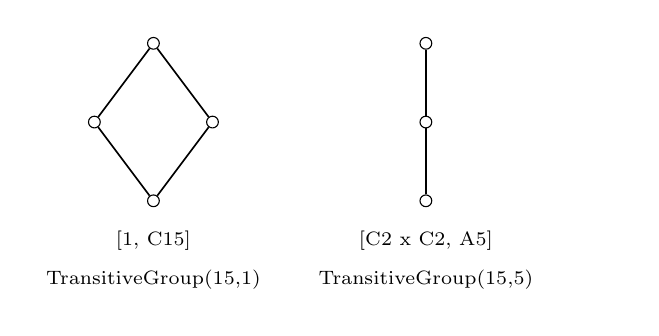
\begin{tikzpicture}[scale=.5]
\matrix[column sep=5mm,row sep=5mm]
{
\node (0) at (0,0) [draw, circle,inner sep=1.5pt] {};
\node (1) at (0.75,1) [draw, circle, inner sep=1.5pt] {};
\node (2) at (-0.75,1) [draw, circle, inner sep=1.5pt] {};
\node (3) at (-0,2) [draw, circle, inner sep=1.5pt] {};
\draw[font=\scriptsize] (0,-.5) node {[1, C15]};
\draw[font=\scriptsize] (0,-1) node {TransitiveGroup(15,1) };

\draw[semithick]
(0) to (1)
(0) to (2)
(1) to (3)
(2) to (3);
&
\node (0) at (0,0) [draw, circle,inner sep=1.5pt] {};
\node (1) at (-0,1) [draw, circle, inner sep=1.5pt] {};
\node (2) at (-0,2) [draw, circle, inner sep=1.5pt] {};
\draw[font=\scriptsize] (0,-.5) node {[C2 x C2, A5]};
\draw[font=\scriptsize] (0,-1) node {TransitiveGroup(15,5) };

\draw[semithick]
(0) to (1)
(1) to (2);
&
& \\
};
\end{tikzpicture}
\end{center}
\end{figure}

\newpage


%\input{TransitiveGsetCongEx16.tex}
%% \input{TransitiveGsetCongEx16CorefreeMin3Max10.tex}
\begin{figure}[h]
\caption{Transitive G-set congruence lattices in Eq(16)}
\label{fig:16}
\begin{center}
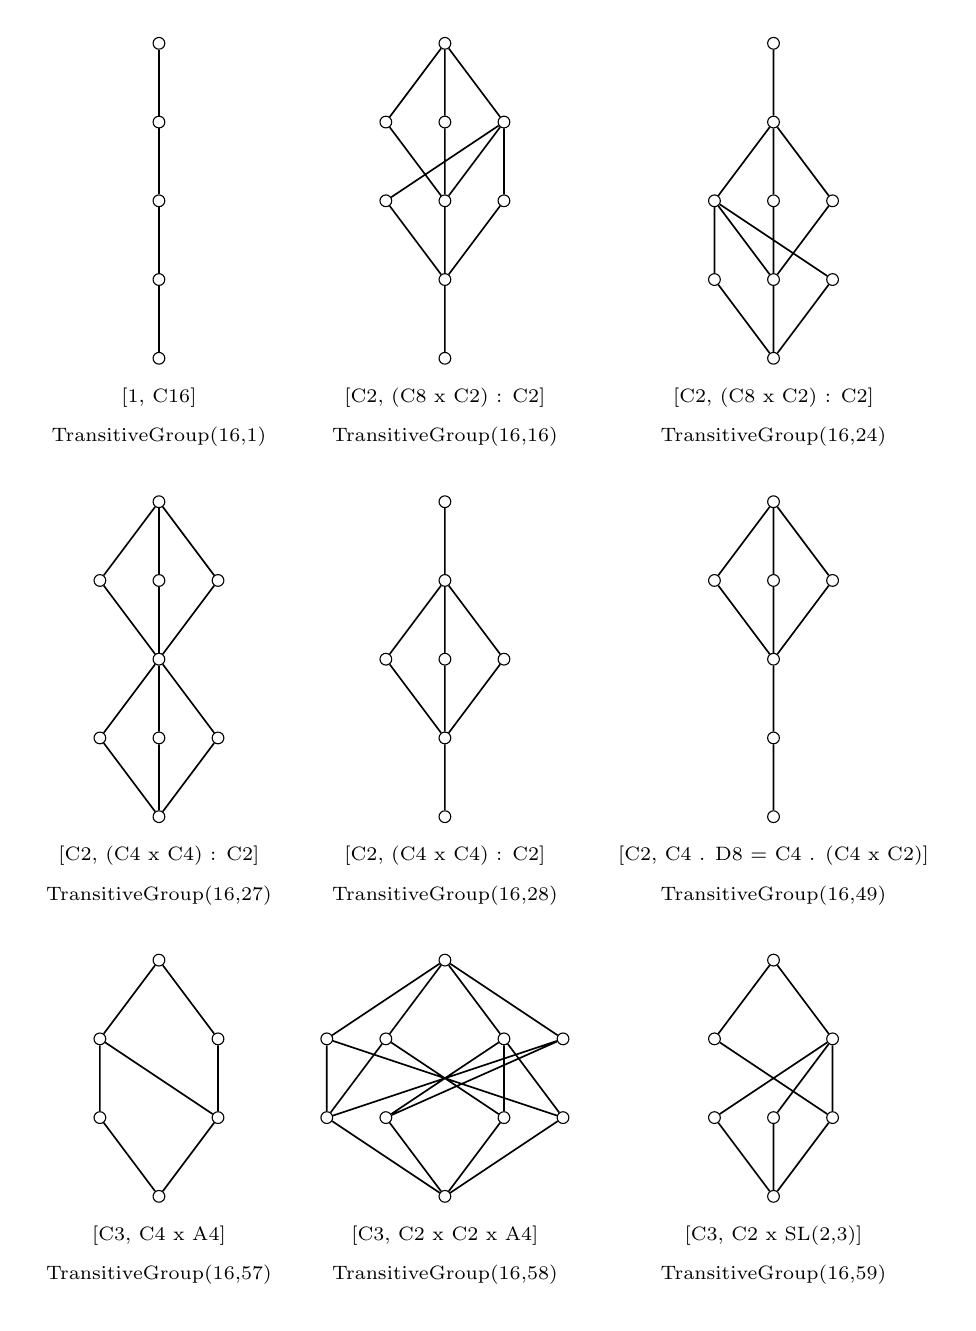
\begin{tikzpicture}[scale=.5]
\matrix[column sep=5mm,row sep=5mm]
{
\node (0) at (0,0) [draw, circle,inner sep=1.5pt] {};
\node (1) at (-0,1) [draw, circle, inner sep=1.5pt] {};
\node (2) at (-0,2) [draw, circle, inner sep=1.5pt] {};
\node (3) at (-0,3) [draw, circle, inner sep=1.5pt] {};
\node (4) at (-0,4) [draw, circle, inner sep=1.5pt] {};
\draw[font=\scriptsize] (0,-.5) node {[1, C16]};
\draw[font=\scriptsize] (0,-1) node {TransitiveGroup(16,1) };

\draw[semithick]
(0) to (1)
(1) to (2)
(2) to (3)
(3) to (4);
&
\node (0) at (0,0) [draw, circle,inner sep=1.5pt] {};
\node (1) at (-0,1) [draw, circle, inner sep=1.5pt] {};
\node (2) at (-0,2) [draw, circle, inner sep=1.5pt] {};
\node (3) at (0.75,2) [draw, circle, inner sep=1.5pt] {};
\node (4) at (-0.75,2) [draw, circle, inner sep=1.5pt] {};
\node (5) at (-0,3) [draw, circle, inner sep=1.5pt] {};
\node (6) at (0.75,3) [draw, circle, inner sep=1.5pt] {};
\node (7) at (-0.75,3) [draw, circle, inner sep=1.5pt] {};
\node (8) at (-0,4) [draw, circle, inner sep=1.5pt] {};
\draw[font=\scriptsize] (0,-.5) node {[C2, (C8 x C2) : C2]};
\draw[font=\scriptsize] (0,-1) node {TransitiveGroup(16,16) };

\draw[semithick]
(0) to (1)
(1) to (2)
(1) to (3)
(1) to (4)
(2) to (5)
(2) to (6)
(2) to (7)
(3) to (6)
(4) to (6)
(5) to (8)
(6) to (8)
(7) to (8);
&
\node (0) at (0,0) [draw, circle,inner sep=1.5pt] {};
\node (1) at (-0,1) [draw, circle, inner sep=1.5pt] {};
\node (2) at (0.75,1) [draw, circle, inner sep=1.5pt] {};
\node (3) at (-0.75,1) [draw, circle, inner sep=1.5pt] {};
\node (4) at (-0,2) [draw, circle, inner sep=1.5pt] {};
\node (5) at (0.75,2) [draw, circle, inner sep=1.5pt] {};
\node (6) at (-0.75,2) [draw, circle, inner sep=1.5pt] {};
\node (7) at (-0,3) [draw, circle, inner sep=1.5pt] {};
\node (8) at (-0,4) [draw, circle, inner sep=1.5pt] {};
\draw[font=\scriptsize] (0,-.5) node {[C2, (C8 x C2) : C2]};
\draw[font=\scriptsize] (0,-1) node {TransitiveGroup(16,24) };

\draw[semithick]
(0) to (1)
(0) to (2)
(0) to (3)
(1) to (4)
(1) to (5)
(1) to (6)
(2) to (6)
(3) to (6)
(4) to (7)
(5) to (7)
(6) to (7)
(7) to (8);
\\
\node (0) at (0,0) [draw, circle,inner sep=1.5pt] {};
\node (1) at (-0,1) [draw, circle, inner sep=1.5pt] {};
\node (2) at (0.75,1) [draw, circle, inner sep=1.5pt] {};
\node (3) at (-0.75,1) [draw, circle, inner sep=1.5pt] {};
\node (4) at (-0,2) [draw, circle, inner sep=1.5pt] {};
\node (5) at (-0,3) [draw, circle, inner sep=1.5pt] {};
\node (6) at (0.75,3) [draw, circle, inner sep=1.5pt] {};
\node (7) at (-0.75,3) [draw, circle, inner sep=1.5pt] {};
\node (8) at (-0,4) [draw, circle, inner sep=1.5pt] {};
\draw[font=\scriptsize] (0,-.5) node {[C2, (C4 x C4) : C2]};
\draw[font=\scriptsize] (0,-1) node {TransitiveGroup(16,27) };

\draw[semithick]
(0) to (1)
(0) to (2)
(0) to (3)
(1) to (4)
(2) to (4)
(3) to (4)
(4) to (5)
(4) to (6)
(4) to (7)
(5) to (8)
(6) to (8)
(7) to (8);
&
\node (0) at (0,0) [draw, circle,inner sep=1.5pt] {};
\node (1) at (-0,1) [draw, circle, inner sep=1.5pt] {};
\node (2) at (-0,2) [draw, circle, inner sep=1.5pt] {};
\node (3) at (0.75,2) [draw, circle, inner sep=1.5pt] {};
\node (4) at (-0.75,2) [draw, circle, inner sep=1.5pt] {};
\node (5) at (-0,3) [draw, circle, inner sep=1.5pt] {};
\node (6) at (-0,4) [draw, circle, inner sep=1.5pt] {};
\draw[font=\scriptsize] (0,-.5) node {[C2, (C4 x C4) : C2]};
\draw[font=\scriptsize] (0,-1) node {TransitiveGroup(16,28) };

\draw[semithick]
(0) to (1)
(1) to (2)
(1) to (3)
(1) to (4)
(2) to (5)
(3) to (5)
(4) to (5)
(5) to (6);
&
\node (0) at (0,0) [draw, circle,inner sep=1.5pt] {};
\node (1) at (-0,1) [draw, circle, inner sep=1.5pt] {};
\node (2) at (-0,2) [draw, circle, inner sep=1.5pt] {};
\node (3) at (-0,3) [draw, circle, inner sep=1.5pt] {};
\node (4) at (0.75,3) [draw, circle, inner sep=1.5pt] {};
\node (5) at (-0.75,3) [draw, circle, inner sep=1.5pt] {};
\node (6) at (-0,4) [draw, circle, inner sep=1.5pt] {};
\draw[font=\scriptsize] (0,-.5) node {[C2, C4 . D8 = C4 . (C4 x C2)]};
\draw[font=\scriptsize] (0,-1) node {TransitiveGroup(16,49) };

\draw[semithick]
(0) to (1)
(1) to (2)
(2) to (3)
(2) to (4)
(2) to (5)
(3) to (6)
(4) to (6)
(5) to (6);
\\
\node (0) at (0,0) [draw, circle,inner sep=1.5pt] {};
\node (1) at (0.75,1) [draw, circle, inner sep=1.5pt] {};
\node (2) at (0.75,2) [draw, circle, inner sep=1.5pt] {};
\node (3) at (-0.75,1) [draw, circle, inner sep=1.5pt] {};
\node (4) at (-0.75,2) [draw, circle, inner sep=1.5pt] {};
\node (5) at (-0,3) [draw, circle, inner sep=1.5pt] {};
\draw[font=\scriptsize] (0,-.5) node {[C3, C4 x A4]};
\draw[font=\scriptsize] (0,-1) node {TransitiveGroup(16,57) };

\draw[semithick]
(0) to (1)
(0) to (3)
(1) to (2)
(1) to (4)
(2) to (5)
(3) to (4)
(4) to (5);
&
\node (0) at (0,0) [draw, circle,inner sep=1.5pt] {};
\node (1) at (0.75,1) [draw, circle, inner sep=1.5pt] {};
\node (2) at (-0.75,1) [draw, circle, inner sep=1.5pt] {};
\node (3) at (1.5,1) [draw, circle, inner sep=1.5pt] {};
\node (4) at (-1.5,1) [draw, circle, inner sep=1.5pt] {};
\node (5) at (0.75,2) [draw, circle, inner sep=1.5pt] {};
\node (6) at (-0.75,2) [draw, circle, inner sep=1.5pt] {};
\node (7) at (1.5,2) [draw, circle, inner sep=1.5pt] {};
\node (8) at (-1.5,2) [draw, circle, inner sep=1.5pt] {};
\node (9) at (-0,3) [draw, circle, inner sep=1.5pt] {};
\draw[font=\scriptsize] (0,-.5) node {[C3, C2 x C2 x A4]};
\draw[font=\scriptsize] (0,-1) node {TransitiveGroup(16,58) };

\draw[semithick]
(0) to (1)
(0) to (2)
(0) to (3)
(0) to (4)
(1) to (5)
(1) to (6)
(2) to (5)
(2) to (7)
(3) to (5)
(3) to (8)
(4) to (6)
(4) to (7)
(4) to (8)
(5) to (9)
(6) to (9)
(7) to (9)
(8) to (9);
&
\node (0) at (0,0) [draw, circle,inner sep=1.5pt] {};
\node (1) at (-0,1) [draw, circle, inner sep=1.5pt] {};
\node (2) at (0.75,1) [draw, circle, inner sep=1.5pt] {};
\node (3) at (-0.75,1) [draw, circle, inner sep=1.5pt] {};
\node (4) at (0.75,2) [draw, circle, inner sep=1.5pt] {};
\node (5) at (-0.75,2) [draw, circle, inner sep=1.5pt] {};
\node (6) at (-0,3) [draw, circle, inner sep=1.5pt] {};
\draw[font=\scriptsize] (0,-.5) node {[C3, C2 x SL(2,3)]};
\draw[font=\scriptsize] (0,-1) node {TransitiveGroup(16,59) };

\draw[semithick]
(0) to (1)
(0) to (2)
(0) to (3)
(1) to (4)
(2) to (4)
(2) to (5)
(3) to (4)
(4) to (6)
(5) to (6);
\\
};
\end{tikzpicture}
\end{center}
\end{figure}

\newpage

\begin{figure}[h]
\caption{Transitive G-set congruence lattices in Eq(16) (continued)}
\label{fig:16b}
\begin{center}
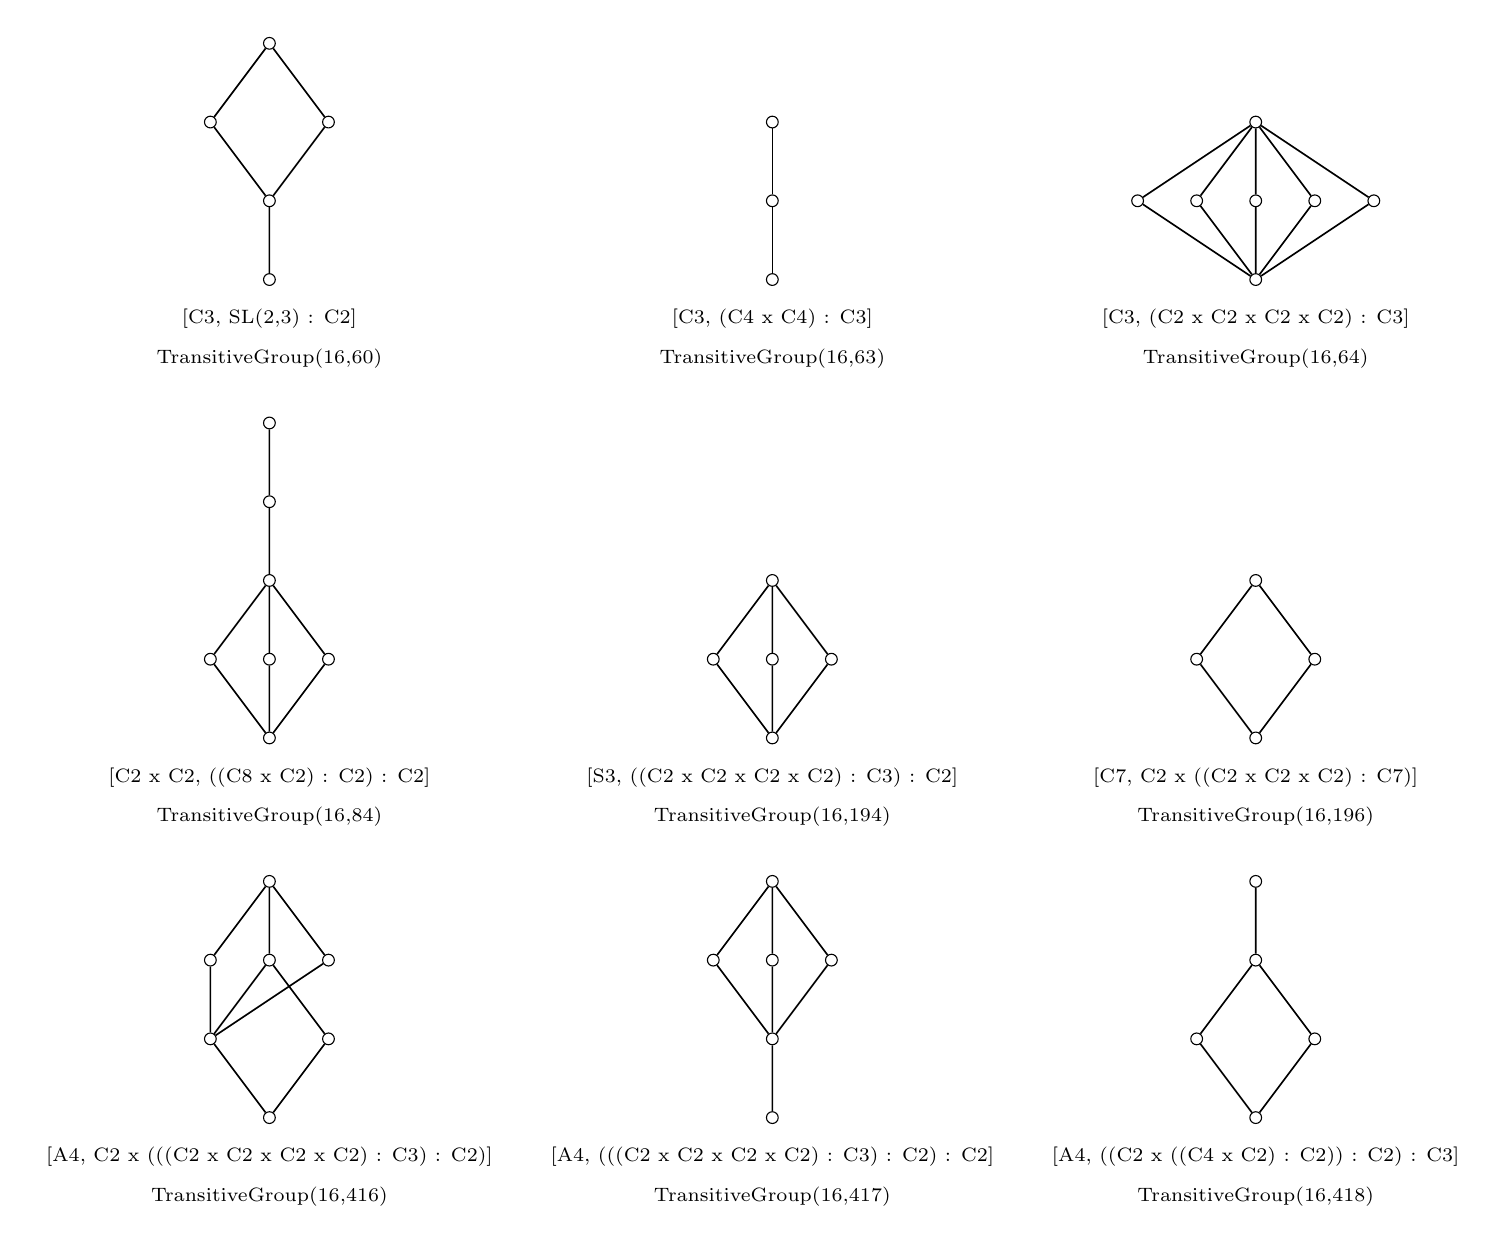
\begin{tikzpicture}[scale=.5]
\matrix[column sep=5mm,row sep=5mm]
{
\node (0) at (0,0) [draw, circle,inner sep=1.5pt] {};
\node (1) at (-0,1) [draw, circle, inner sep=1.5pt] {};
\node (2) at (0.75,2) [draw, circle, inner sep=1.5pt] {};
\node (3) at (-0.75,2) [draw, circle, inner sep=1.5pt] {};
\node (4) at (-0,3) [draw, circle, inner sep=1.5pt] {};
\draw[font=\scriptsize] (0,-.5) node {[C3, SL(2,3) : C2]};
\draw[font=\scriptsize] (0,-1) node {TransitiveGroup(16,60) };

\draw[semithick]
(0) to (1)
(1) to (2)
(1) to (3)
(2) to (4)
(3) to (4);
&
\node (0) at (0,0) [draw, circle,inner sep=1.5pt] {};
\node (1) at (-0,1) [draw, circle, inner sep=1.5pt] {};
\node (2) at (-0,2) [draw, circle, inner sep=1.5pt] {};
\draw[font=\scriptsize] (0,-.5) node {[C3, (C4 x C4) : C3]};
\draw[font=\scriptsize] (0,-1) node {TransitiveGroup(16,63) };

\draw[semithick]
(0) to (1)
(1) to (2);
&
\node (0) at (0,0) [draw, circle,inner sep=1.5pt] {};
\node (1) at (-0,1) [draw, circle, inner sep=1.5pt] {};
\node (2) at (0.75,1) [draw, circle, inner sep=1.5pt] {};
\node (3) at (-0.75,1) [draw, circle, inner sep=1.5pt] {};
\node (4) at (1.5,1) [draw, circle, inner sep=1.5pt] {};
\node (5) at (-1.5,1) [draw, circle, inner sep=1.5pt] {};
\node (6) at (-0,2) [draw, circle, inner sep=1.5pt] {};
\draw[font=\scriptsize] (0,-.5) node {[C3, (C2 x C2 x C2 x C2) : C3]};
\draw[font=\scriptsize] (0,-1) node {TransitiveGroup(16,64) };

\draw[semithick]
(0) to (1)
(0) to (2)
(0) to (3)
(0) to (4)
(0) to (5)
(1) to (6)
(2) to (6)
(3) to (6)
(4) to (6)
(5) to (6);
\\
\node (0) at (0,0) [draw, circle,inner sep=1.5pt] {};
\node (1) at (-0,1) [draw, circle, inner sep=1.5pt] {};
\node (2) at (0.75,1) [draw, circle, inner sep=1.5pt] {};
\node (3) at (-0.75,1) [draw, circle, inner sep=1.5pt] {};
\node (4) at (-0,2) [draw, circle, inner sep=1.5pt] {};
\node (5) at (-0,3) [draw, circle, inner sep=1.5pt] {};
\node (6) at (-0,4) [draw, circle, inner sep=1.5pt] {};
\draw[font=\scriptsize] (0,-.5) node {[C2 x C2, ((C8 x C2) : C2) : C2]};
\draw[font=\scriptsize] (0,-1) node {TransitiveGroup(16,84) };

\draw[semithick]
(0) to (1)
(0) to (2)
(0) to (3)
(1) to (4)
(2) to (4)
(3) to (4)
(4) to (5)
(5) to (6);
&
\node (0) at (0,0) [draw, circle,inner sep=1.5pt] {};
\node (1) at (-0,1) [draw, circle, inner sep=1.5pt] {};
\node (2) at (0.75,1) [draw, circle, inner sep=1.5pt] {};
\node (3) at (-0.75,1) [draw, circle, inner sep=1.5pt] {};
\node (4) at (-0,2) [draw, circle, inner sep=1.5pt] {};
\draw[font=\scriptsize] (0,-.5) node {[S3, ((C2 x C2 x C2 x C2) : C3) : C2]};
\draw[font=\scriptsize] (0,-1) node {TransitiveGroup(16,194) };

\draw[semithick]
(0) to (1)
(0) to (2)
(0) to (3)
(1) to (4)
(2) to (4)
(3) to (4);
&
\node (0) at (0,0) [draw, circle,inner sep=1.5pt] {};
\node (1) at (0.75,1) [draw, circle, inner sep=1.5pt] {};
\node (2) at (-0.75,1) [draw, circle, inner sep=1.5pt] {};
\node (3) at (-0,2) [draw, circle, inner sep=1.5pt] {};
\draw[font=\scriptsize] (0,-.5) node {[C7, C2 x ((C2 x C2 x C2) : C7)]};
\draw[font=\scriptsize] (0,-1) node {TransitiveGroup(16,196) };

\draw[semithick]
(0) to (1)
(0) to (2)
(1) to (3)
(2) to (3);
\\
\node (0) at (0,0) [draw, circle,inner sep=1.5pt] {};
\node (1) at (0.75,1) [draw, circle, inner sep=1.5pt] {};
\node (2) at (-0.75,1) [draw, circle, inner sep=1.5pt] {};
\node (3) at (-0,2) [draw, circle, inner sep=1.5pt] {};
\node (4) at (0.75,2) [draw, circle, inner sep=1.5pt] {};
\node (5) at (-0.75,2) [draw, circle, inner sep=1.5pt] {};
\node (6) at (-0,3) [draw, circle, inner sep=1.5pt] {};
\draw[font=\scriptsize] (0,-.5) node {[A4, C2 x (((C2 x C2 x C2 x C2) : C3) : C2)]};
\draw[font=\scriptsize] (0,-1) node {TransitiveGroup(16,416) };

\draw[semithick]
(0) to (1)
(0) to (2)
(1) to (3)
(2) to (3)
(2) to (4)
(2) to (5)
(3) to (6)
(4) to (6)
(5) to (6);
&
\node (0) at (0,0) [draw, circle,inner sep=1.5pt] {};
\node (1) at (-0,1) [draw, circle, inner sep=1.5pt] {};
\node (2) at (-0,2) [draw, circle, inner sep=1.5pt] {};
\node (3) at (0.75,2) [draw, circle, inner sep=1.5pt] {};
\node (4) at (-0.75,2) [draw, circle, inner sep=1.5pt] {};
\node (5) at (-0,3) [draw, circle, inner sep=1.5pt] {};
\draw[font=\scriptsize] (0,-.5) node {[A4, (((C2 x C2 x C2 x C2) : C3) : C2) : C2]};
\draw[font=\scriptsize] (0,-1) node {TransitiveGroup(16,417) };

\draw[semithick]
(0) to (1)
(1) to (2)
(1) to (3)
(1) to (4)
(2) to (5)
(3) to (5)
(4) to (5);
&
\node (0) at (0,0) [draw, circle,inner sep=1.5pt] {};
\node (1) at (0.75,1) [draw, circle, inner sep=1.5pt] {};
\node (2) at (-0.75,1) [draw, circle, inner sep=1.5pt] {};
\node (3) at (-0,2) [draw, circle, inner sep=1.5pt] {};
\node (4) at (-0,3) [draw, circle, inner sep=1.5pt] {};
\draw[font=\scriptsize] (0,-.5) node {[A4, ((C2 x ((C4 x C2) : C2)) : C2) : C3]};
\draw[font=\scriptsize] (0,-1) node {TransitiveGroup(16,418) };

\draw[semithick]
(0) to (1)
(0) to (2)
(1) to (3)
(2) to (3)
(3) to (4);
\\
};
\end{tikzpicture}
\end{center}
\end{figure}

\newpage

\begin{figure}[h]
\caption{Transitive G-set congruence lattices in Eq(16) (continued)}
\label{fig:16c}
\begin{center}
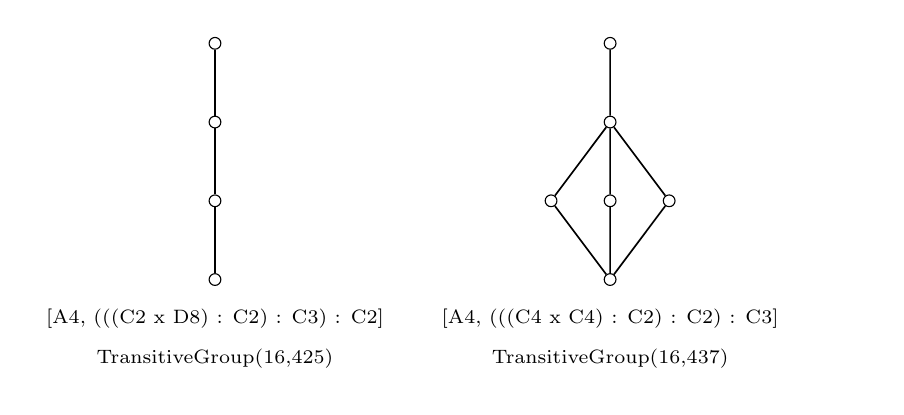
\begin{tikzpicture}[scale=.5]
\matrix[column sep=5mm,row sep=5mm]
{
\node (0) at (0,0) [draw, circle,inner sep=1.5pt] {};
\node (1) at (-0,1) [draw, circle, inner sep=1.5pt] {};
\node (2) at (-0,2) [draw, circle, inner sep=1.5pt] {};
\node (3) at (-0,3) [draw, circle, inner sep=1.5pt] {};
\draw[font=\scriptsize] (0,-.5) node {[A4, (((C2 x D8) : C2) : C3) : C2]};
\draw[font=\scriptsize] (0,-1) node {TransitiveGroup(16,425) };

\draw[semithick]
(0) to (1)
(1) to (2)
(2) to (3);
&
\node (0) at (0,0) [draw, circle,inner sep=1.5pt] {};
\node (1) at (-0,1) [draw, circle, inner sep=1.5pt] {};
\node (2) at (0.75,1) [draw, circle, inner sep=1.5pt] {};
\node (3) at (-0.75,1) [draw, circle, inner sep=1.5pt] {};
\node (4) at (-0,2) [draw, circle, inner sep=1.5pt] {};
\node (5) at (-0,3) [draw, circle, inner sep=1.5pt] {};
\draw[font=\scriptsize] (0,-.5) node {[A4, (((C4 x C4) : C2) : C2) : C3]};
\draw[font=\scriptsize] (0,-1) node {TransitiveGroup(16,437) };

\draw[semithick]
(0) to (1)
(0) to (2)
(0) to (3)
(1) to (4)
(2) to (4)
(3) to (4)
(4) to (5);
&
& \\
};
\end{tikzpicture}
\end{center}
\end{figure}

\newpage


%\input{TransitiveGsetCongEx16CorefreeMin3Max14.tex}



\newpage
%% \section{Permutation Groups}
\section{Group actions and permutation groups}
Let $\bG$ be a group, $\bA= \<A; \barG\>$ a \Gset, and let $\Sym(A)$ denote the group of
permutations of $A$.
For $a\in A$, the one-generated subalgebra $\<a\>\in \Sub[\bA]$ is
called the \defin{orbit} of $a$ in $\bA$. 
It is easily verified that $\<a\>$ is the set
$ \barG a :=  \{\barg a \mid g\in G\}$, and we often use the more suggestive 
$\barG a$ when referring to this orbit.

The orbits of the \Gset\ $\bA$ partition the set $A$ into disjoint
equivalence classes.  The equivalence relation $\sim$ is defined on $A^2$ as follows: 
$x \sim y$ iff $\barg x = y$ for some $g\in G$.
In fact, $\sim$ is a congruence relation of the algebra $\bA$ since,
$x \sim y$ implies $\barg x \sim \barg y$.
Thus, as mentioned above, each orbit is indeed a \emph{subalgebra} of $\bA$.

Keep in mind that $A$ is the disjoint union of the
orbits.  That is, if $\{a_1, \dots, a_r\}$ is a full
set of $\sim$-class representatives, then $A = \bigcup_{i=1}^r \barG a_i$ is a disjoint union.

A \Gset\ with only one orbit is called 
\defin{transitive}.  Equivalently, $\<A, \barG\>$ is a transitive \Gset\ iff 
$(\forall a, b \in A)(\exists g\in G)(\barg a = b)$. 
In this case, we say that $\bG$ \emph{acts transitively} on $A$,
and occasionally we refer to the group $G$ itself as a \emph{transitive group} of \emph{degree} $|A|$.  

For $a\in A$, the set $\Stab_G(a) := \{g \in G \mid  \barg a  = a\}$ is called the 
\defin{stabilizer} of $a$.  It is easy to verify  that $\Stab_G(a)$ is a
subgroup of $\bG$.  An alternative notation for the stabilizer 
is $G_a := \Stab_G(a)$.

Let $\lambda : \bG \rightarrow \barG \leq \Sym(A)$ denote the permutation representation
of $\bG$; that is, $\lambda(g) = \barg$. Then 
\begin{equation}
  \label{eq:111}
\ker \lambda = \{g\in G  \mid  \barg a = a \text{ for all $a\in A$}\} = \bigcap_{a\in A}
\Stab_G(a)
= \bigcap_{a\in A} G_a.
\end{equation}
Therefore, $\bG/\ker\lambda \cong \lambda[G]\leq \Sym(A)$.
We say that the representation $\lambda$ of $\bG$ is \defin{faithful}, or 
that $\bG$ \emph{acts faithfully} on $A$, just in case $\ker \lambda = 1$. In
this case $\lambda : \bG \hookrightarrow \Sym(A)$, so $\bG$ itself is isomorphic to a subgroup of 
$\Sym(A)$, and we call $\bG$ a \defin{permutation group}.

If $H \leq G$ are groups, the \defin{core} of $H$ in $G$, denoted $\core_G(H)$,
is the largest normal subgroup of $G$ that is contained in $H$.  It is easy to see
that
\[
\core_G(H) = \bigcap_{g\in G}g H g^{-1}.
\]
A subgroup $H$ is called \emph{core-free} provided $\core_G(H)=1$.

Elements in the same orbit of a \Gset\
have conjugate stabilizers.  Specifically, if $a, b\in A$  and $g\in G$ are
such that $\barg a = b$, then 
$\stab{b} = \stab{\barg a} = g \,\stab{a}\, g^{-1}$.
If the \Gset\ happens to be transitive, then it is faithful iff the stabilizer $\stab{a}$
is core-free in $G$. For,
%To see this, note that if $G$ acts transitively, then $\barG a = A$ and
\[
\ker \lambda = \bigcap_{a\in A} \stab{a}
= \bigcap_{g\in G} \stab{\barg a}
= \bigcap_{g\in G} g \,\stab{a}  \,g^{-1}.
\]
Thus $\stab{a}$ is core-free iff $\ker \lambda = 1$ iff $G$ acts faithfully on $A$.

In case $\bG$ is a transitive permutation group, we say that $\bG$ is 
\defin{regular} (or that $\bG$ \emph{acts regularly} on $A$, or that $\lambda
: G \rightarrow \barG$ is a \emph{regular representation})
provided $\stab{a} = 1$ for each $a\in A$; i.e.,
every non-identity element of $G$ is fixed-point-free.\footnote{The action of a
  regular permutation group is sometimes called a ``free'' action.} Equivalently,
$G$ is regular on $A$ iff for each $a, b \in A$ there is a unique $g\in G$ such
that $\barg a = b$.  In particular, $|G| = |A|$.

A \defin{block system} for $G$ is a partition of $A$
  that is preserved by the action of $G$.  In other words, a block system is a
  congruence relation of the algebra $\bA = \<A,\barG\>$.
The \defin{trivial block systems} are $0_A = |a_1|a_2|\cdots|a_i|\cdots$ and 
$1_A = |a_1 a_2 \cdots a_i \cdots|$.  The non-trivial block systems are called \defin{systems of imprimitivity}.

A nonempty subset $B\subseteq A$ is a \defin{block} for $\bA$ 
if for each $g \in G$ either $\barg B = B$ or $\barg B \cap B = \emptyset$.

Let $\bA = \<A, \barG\>$ be a transitive \Gset.  
We say that the group $\bG$ is \defin{primitive} if $\bA$ has no systems of imprimitivity;
otherwise $\bG$ is called \defin{imprimitive}. 
Note that we only use the terms ``primitive'' and ``imprimitive''
with reference to a \emph{transitive} \Gset.

%% \item[{\small {\it blocks}}] Let $\bA = \<A,\barG\>$ be a transitive \Gset.
%% A nonempty subset $B\subseteq A$ is called a \defin{block} for $\bA$ 
%% if for each $g \in G$ either $\barg B = B$ or $\barg B \cap B = \emptyset$.  (We will
%% call such $B$ a block if the underlying \Gset\ is clear from context.)

%% For example, every transitive \Gset\ $\<A, \barG\>$ has $A$ and the 
%% singletons $\{a\}\; (a \in A)$ as blocks; these are called the 
%% \emph{trivial blocks}. Any other block is called \emph{nontrivial}. 
%% A block which is minimal in the set of all blocks of size $> 1$ is called a
%% \emph{minimal block}. 

%% If $B$ and $C$ are blocks of a transitive \Gset\
%% containing a common point, then $B \cap C$ is also a block. More,
%% generally, any intersection of blocks containing a common point is again a
%% block.

%% The importance of blocks arises from the following observation. 
%% Suppose that $\bA = \<A,\barG\>$ is a transitive \Gset\ 
%% and that $B$ is a block for $\bA$.  
%% Put $\beta = \{\barg B  \mid  g\in G\}$. 
%% Then the sets in $\beta$ form a partition of $A$ 
%% and each element of $\beta$ is a block. 
%% We call $\beta$ the system of blocks containing $B$.
%% Now $\bG$ acts on $\beta$ in an obvious way, and this new action may give useful
%% information about $\bG$ provided $B$ is not a trivial block.


%%% The following is already included in the body:
%% \begin{theorem}
%% Let $\bA = \<A,\barG\>$ be a transitive \Gset\
%% and let $a \in A$. Let $\sB$ be the set of all blocks $B$ with $a\in B$.
%% Let $[\stab{a},G] \subseteq \Sub[\bG]$ denote the set of all subgroups of $\bG$ 
%% containing $\stab{a}$.  Then there is a
%% bijection $\Psi :\sB \rightarrow [\stab{a},G]$ given by $\Psi(B)= G(B)$,
%% with inverse mapping $\Phi: [\stab{a},G] \rightarrow \sB $ 
%% given by $\Phi(H) = \barH a = \{\barh a  \mid  h\in H\}$. 
%% The mapping $\Psi$ is order-preserving in the sense
%% that if $B_1, B_2 \in  \sB$ then 
%% $B_1\subseteq B_2 \Leftrightarrow \Psi(B_1) \leq \Psi(B_2)$.
%% \end{theorem}
%% Briefly, the poset $\<\sB, \subseteq\>$ is order-isomorphic to the poset $\<[\stab{a},G], \leq \>$.

%% \begin{corollary}
%% Let $\bG$ act transitively on a set with at least two points.
%% %$\bA = \<A, \barG\>$ be a transitive \Gset\ with on a set n with at
%% Then $\bG$ is primitive if and only if each stabilizer $\stab{a}$ is a
%% maximal subgroup of $\bG$.
%% \end{corollary}

%% Since the point stabilizers of a transitive group are all conjugate, 
%% one stabilizer is maximal only when all of the stabilizers are maximal. 
%% In particular, a regular permutation group is primitive if and only if it has prime
%% degree. 




\newpage

\section{Classifying permutation groups}
\label{sec:class-perm-groups}
A permutation group is either transitive
or is a subdirect product of transitive groups, while a transitive group is
either primitive or is a subgroup of an iterated wreath product of primitive
groups. (Iterated wreath products are discussed in section~\ref{sec:quas-groups} below.)
Hence primitive groups can be viewed as the building blocks of all
permutations groups and their classification helps us to better understand
the structure of permutation groups in general.

The \defn{socle} of a group $G$ is the subgroup generated by the minimal normal
subgroups of $G$ and is denoted by $\Soc(G)$. By~\cite{Dixon:1996}, Corollary 4.3B, the socle
of a finite primitive group is isomorphic to the direct product of one or more
copies of a simple group $T$.  The O'Nan-Scott Theorem classifies the primitive
permutation groups according to the structure of their socles.  This section
sets up the background for the statement and proof of the theorem. The
theorem itself is presented in section~\ref{sec:onan-scott-theorem}.

\subsection{Preliminary definitions and lemmas}
Two permutation representations 
$\rho : G \rightarrow \Sym(\Omega)$ and
$\lambda : G \rightarrow \Sym(\Gamma)$ are \defn{equivalent} provided $|\Omega| =
|\Gamma|$ and there exists a $G$-set isomorphism
\[
\sigma : \<\Omega, \{\rho(g) : g\in G\}\> \rightarrow 
\<\Gamma, \{\lambda(g) : g\in G\}\>.
\]
That is  $\sigma: \Omega \rightarrow 
\Gamma$ satisfies $\sigma(\omega^{\rho(g)}) = (\sigma(\omega))^{\lambda(g)}$ for
all $\omega \in \Omega$ and $g \in G$.

A subgroup $K$ of a group $G$ is called \defn{characteristic} if it is fixed by all
automorphisms of $G$.
A group $K \neq 1$ is called characteristically simple if $K$ has no proper 
non-trivial characteristic subgroups.  The following are easily verified:
\begin{enumerate}[(a)]
\item If $K \subnormal N \subnormal G$ and $K$ is characteristic in $N$ then
  $K\subnormal G$.
\item If $N_1 \neq N_2$ are minimal normal subgroups of a group $G$, then $[N_1,
  N_2]\leq N_1\cap N_2 = 1$, so $N_1$ and $N_2$ commute.
\item If $K$ is characteristically simple then $K\cong T^r$ for some
 simple group $T$. (In particular, minimal normal subgroups are direct powers of
 simple groups.)

\end{enumerate}
%% {\it Proof of (c)}. If $T$ is a minimal normal subgroup of $K$, then so is
%% $T^\alpha$ for any $\alpha \in  \Aut K$. So by (b) either $T^\alpha = T$ or 
%% $T \cap T^\alpha = 1$. 
%% In the latter case
%% $T T^\alpha = T \times T^\alpha$ is a direct product. Since 
%% $K$ is characteristically simple, it is
%% generated by all the $T^\alpha$. By induction we obtain that $K$ is a direct product of
%% a finite number of such $T^\alpha$. But then any normal subgroup of $T$ is normal in
%% $T$, so by minimality of $T$, $T$ is simple.

Let $G$ be a primitive permutation group on an $n$-element set $A$, 
and let $N, N_1, N_2$ be nontrivial normal subgroups of $G$.  Then,
\begin{enumerate}
\item $N$ is transitive. (Otherwise, the orbits of $N$ form a system of
  imprimitivity for $G$.)
\item Either $C_G(N) = 1$, or $C_G(N)$ is regular and $|C_G(N)| = |A|$.
\item If $[N_1, N_2] = 1$ then $N_1 = C_G(N_2)$, $N_2 = C_G(N_1)$, and $N_1
  \cong N_2$.
\item For each $a\in A$, $NG_a = G$.
\item If $N$ is minimal, then $G_a\cap N$ is maximal among $G_a$-invariant
  subgroups of $N$.
\end{enumerate}

The lemmas above appear in Wilson's notes, while the next three results do
not. I believe it is the last of these that enables Wilson to quickly conclude
the affine case of the O'Nan-Scott Theorem. 

\begin{enumerate}[(i)]
\item Suppose $G$ acts transitively on two sets $\Omega$ and $\Gamma$,
and let $H$ be a stabilizer of a point in $\Omega$. Then the representations are
equivalent iff $H$ is a stabilizer of a point in $\Gamma$.

For the next two results, suppose $G$ acts transitively on $\Omega$ and $\alpha \in
\Omega$.

\item A subgroup $N\leq G$ is transitive iff $NG_\alpha = G$.
Also, $N$ is regular iff in addition $N \cap G_\alpha = 1$.

\item Let $H$ be the normalizer of $G$ in $\Sym(\Omega)$, with the usual conjugation
action given by the homomorphism
\[
\Psi : H \rightarrow \Aut(G) \qquad \Psi(n): g \mapsto n^{-1} g n
\]
and fix $\sigma \in \Aut(G)$.  Then
$\sigma \in \Im \Psi$ iff $(G_\alpha)^\sigma = G_\beta$ for some $\beta \in \Omega$.
\end{enumerate}

\begin{corollary}
If $G$ is regular, then $\Aut(G) = \Im \Psi$ and $H_\alpha \cong \Aut(G)$ and $H \cong G \rtimes \Aut(G)$.
\end{corollary}

Let $G$ be a finite primitive subgroup of $\Sym(\Omega)$ with regular minimal normal
subgroup $N$ and fix $\alpha \in \Omega$.  Let $H$ be the normalizer of $N$ in $\Sym(\Omega)$.  
%By (c) above, $N\cong T^m$ for some simple group $T$.
The group $H$ is called the ``holomorph of $N$.'' By the corollary above, $H \cong
N\rtimes \Aut(N)$.  More precisely, the algebra consisting of the point stabilizer $H_\alpha$ acting on
$\Omega$ is isomorphic to the algebra consisting of $\Aut(N)$ acting naturally
on $N$ and $H = N H_\alpha$ with $N\cap H_\alpha = 1$.  Similarly, $G = NG_\alpha$.


\subsection{The O'Nan-Scott Theorem}
\label{sec:onan-scott-theorem}

\begin{theorem}[O'Nan-Scott Theorem, version 1] 
Let $G$ be a primitive permutation
group of degree $d$, and let $H := \Soc(G) \cong T^m$ with $m \geq 1$. 
Then one of the following holds.
\begin{enumerate}
\item 
$H$ is regular and
  \begin{enumerate}
  \item 
  \defn{Affine type} $T$ is cyclic of order $p$, so $|H| = p^m$ . Then 
$d = p^m$ and $G$ is permutation isomorphic to a subgroup of the affine
general linear group $\AGL(m,p)$. We call $G$ a group of \emph{affine type}.
\item \defn{Twisted wreath product type} $m \geq 6$, the group $T$ is 
  nonabelian and $G$ is a group of \emph{twisted wreath product type}, with
  $d = |T|^m$.
  \end{enumerate}
\item $H$ is non-regular and non-abelian and
  \begin{enumerate}
  \item 
\defn{Almost simple} $m = 1$ and $T \leq G \leq \Aut(T)$.
\item \defn{Product action} $m \geq 2$ and $G$ is permutation isomorphic to a
subgroup of the product action wreath product $P \wr S_{m/l}$ of degree
$d = nm/l$. The group $P$ is primitive of type 2.(a) or 2.(c), $P$ has
degree $n$ and $\Soc(P) \cong T^l$, where $l \geq 1$ divides $m$.
\item 
\defn{Diagonal type} $m \geq 2$ and $T^m \leq G \leq T^m . (\Out(T ) \times S_m)$, with
the diagonal action. The degree $d = |T|^{m-1}$.
  \end{enumerate}
\end{enumerate}
\end{theorem}
We can see immediately that there are no twisted wreath product type
groups of degree less than $60^6$ ($=46.656$ billion).
Note that this definition of product action groups is more restrictive
than that given by some authors. This is in order to make the O’Nan-Scott
classes disjoint.
\\\\
{\bf The O'Nan-Scott Theorem (version 2)}
\\
The O'Nan-Scott Theorem classifies the maximal subgroups
of the alternating and symmetric groups. It does not tell us exactly what the
maximal subgroups are -- that is too much to ask -- but it does provide a first
step towards writing down the list of maximal subgroups of $A_n$ or $S_n$ for any
particular reasonable value of $n$.

\begin{theorem}[O'Nan-Scott Theorem, version 2] 
 If $G \leq S_n$ is a permutation group not containing $A_n$, then $G$
is a subgroup of one or more of the following subgroups:
\begin{enumerate}[(i)]
\item An intransitive group $S_k \times S_m$ , where $n = k + m$;
\item An imprimitive group $S_k \wr S_m$ , where $n = km$;
\item A primitive wreath product $S_k \wr S_m$ , where $n = k^m$;
\item An affine group $AGL_d(p) \cong p^d \rtimes GL_d(p)$, where $n=p^d$;
\item A group of shape $T^m.(\Out(T) \times S_m)$, where $T$ is a non-abelian simple
group, acting on the cosets of the ``diagonal'' subgroup $\Aut(T)\times S_m$, where
$n = |T|^{m-1}$;
\item An almost simple group acting on the cosets of a maximal subgroup.
\end{enumerate}
\end{theorem}
Note that the theorem does not assert that all these subgroups are maximal
in $S_n$, or in $A_n$. This is a rather subtle question, particularly as far as subgroups
of $A_n$ are concerned. The last category of subgroups also requires us to know all
the finite simple groups, or at least those with a maximal subgroup of index $n$.
In practice, this means that we can only ever hope to get a recursive description
of the maximal subgroups of $A_n$ and $S_n$.


\subsection{Quasiprimitive groups}
\label{sec:quas-groups}
A permutation group $X$ on a set $\Omega$ is said to be \defn{quasiprimitive} on
$\Omega$ if each of its nontrivial normal subgroups is transitive on $\Omega$.
In~\cite{Praeger:1993}, Praeger gives a structure theorem classifying finite
quasiprimitive permutation groups, along the lines of the
Aschbacher-O'Nan-Scott Theorem for finite primitive permutation groups.
We record this theorem in this section for easy reference.


\begin{theorem}[O'Nan-Scott Theorem, version 3] 
A finite quasiprimitive permutation group is permutationally
equivalent to a group of one of the types I, II, III(a), III(b), and III(c) described below.
\end{theorem}

The group $X$ below will be a quasiprimitive permutation group on a finite set $\Omega$ of size n,
and $\alpha \in \Omega$. Let $B$ be the socle of $X$, that is the product of all
minimal normal subgroups of $X$. Then $B\cong T^k$ with $k \geq 1$ where $T$ is
a simple group. 

\begin{enumerate}
\item[I.] 
\emph{Affine groups.} Here $T= \Z_p$ for some prime $p$, and $B$ is the unique minimal
normal subgroup of $X$ and is regular on $\Omega$. of degree $n = p^k$. The set $\Omega$. can be
identified with $B = \Z_p^k$ so that $X$ is a subgroup of the affine group $\AGL(k,p)$ with $B$
the translation group and $X_\alpha = X \cap \GL(k,p)$ irreducible on $B$. Moreover $X$ is
primitive on $\Omega$.
\item[II.] \emph{Almost simple groups.} Here $k = 1$, $T$ is a nonabelian simple group,
$T \leq X \leq \Aut T$ and $X = T X_\alpha$.
\item[III.] In this case $B \cong T^k$ with $k\geq 2$ and $T$ a nonabelian simple group. We
distinguish three types:
\begin{enumerate}
\item[III(a).] \emph{Simple diagonal action.} Define
\[
W = \{(a_1,\dots, a_k) \cdot \pi \mid a_i\in  \Aut T,\; \pi \in S_k, \;
a_i \equiv a \mod \Inn T \text{ for all } i, j\},
\]
where $\pi \in S_k$ just permutes the components $a_i$ naturally. 
With the obvious multiplication, $W$ is a group with socle $B\cong T^k$, 
and $W = B . (\Out T\times S_k)$, a (not
necessarily split) extension of $B$ by $\Out T \times S_k$. 
We define an action of $W$ on $\Omega$ by setting
\[
W_\alpha = \{(a,\dots,a)\cdot \pi \mid a\in \Aut T, \, \pi \in S_k\}.
\]
Thus $W_a \cong \Aut T \times S_k$, $B_\alpha \cong T$ and $n = |T|^{k-1}$.

For $1 \leq  i \leq k$ let $T_i$ be the subgroup of $B$ consisting of the
$k$-tuples with 1 in all but the $i$th component, so that 
$T_i \cong T$ and $B \cong T_1 \times \cdots \times T_k$. Put $\sT = \{T_1,
\dots, T_k\}$, so that $W$ acts on $\sT$. 
We say that the subgroup $X$ of $W$ is of type III(a) $B\leq X$ and,
letting $P$ be the permutation group $X^\sT$, one of the following holds:
\begin{enumerate}[(i)]
\item $P$ is transitive on $\sT$,
\item $k = 2$ and $P= 1$.
\end{enumerate}
We have $X_\alpha\leq  \Aut T \times P$, and $X\leq B. (\Out T\times P)$. 
Moreover, in case (i) $B$ is the \emph{unique} minimal normal subgroup of $X$ and $X$ is
primitive on $\Omega$ if and only if $P$ is primitive on $\sT$. 
In case (ii) $X$ has two minimal normal subgroups $T_1$ and $T_2$, both
regular on $\Omega$, and $X$ is primitive on $\Omega$.
\item[III(b).] \emph{Product action.} Let $H$ be a quasiprimitive permutation group on a set $\Gamma$,
  of type II or III(a). For $\ell > 1$, let $W = H \wr S_\ell$,, and take $W$ to
  act on $\Gamma^\ell$ in its natural product action. Then for
  $\gamma\in T$ and $\delta = (\gamma,\dots,\gamma)\in \Gamma^\ell$ we have
  $W_\delta = H_\gamma \wr S_\ell$.  If $K$ is the socle of $H$ then the socle
  $B$ of $W$ is $K^\ell$.

Now $W$ acts naturally on the $\ell$ factors in $K^l$, and we say that a subgroup $X$ of $W$
is of type III(b) if $B\leq X$, $X$ acts transitively on these $\ell$ factors, and one of the
following holds:
\begin{enumerate}[(i)]
\item 
$H$ is of type II, $K\cong T$, $k = \ell$, and $B$ is the unique minimal normal subgroup
of $X$; further $\Gamma^\ell$ is an $X$-invariant partition of $\Omega$ and, for
$\alpha$ in the part $\delta \in \Gamma^\ell$,
$B_\delta = T_\gamma^k < B$ and for some nontrivial normal subgroup $R$ of
$T_\gamma$, $B_\alpha$ is a
subdirect product of $R^k$.
\item 
$H$ is of type III(a), $\Omega = \Gamma^\ell$, $K\cong T^{k/\ell}$ and $X$ and $H$ both have $m$ minimal
normal subgroups where $m \leq 2$; if $m = 2$ then each of the two minimal
normal subgroups of $X$ is regular on $\Omega$.
\end{enumerate}
\item[III(c).] \emph{Twisted wreath action.} Here $X$ is a twisted wreath
  product $T \wr_\phi P$, defined
as follows. (The original construction is due to B.~H.~Neumann~\cite{Neumann:1963}; 
here we follow \cite{Suzuki:1982}, p.~269.) 
Let $P$ have a transitive action on $\{1,...,k\}$ and let $Q$ be the stabilizer $P_1$ of
the point $1$ in this action. We suppose that there is a homomorphism $\phi : Q \rightarrow \Aut T$
such that $\core_P (\phi^{-1}(\Inn T)) = \bigcap_{x\in P} \phi^{-1}(\Inn T)^x = 1$. Define
\[
B = \{f:P\rightarrow T \mid f(pq) =f(p)^{\phi(q)} \text{ for all }
p\in P, q\in Q\}.
\]
Then $B$ is a group under point-wise multiplication, and $B \cong T^k$. Let $P$
act on $B$ by
\[
f^p(x)=f(px) \quad \text{ for $p,x \in P$.}
\]
We define $T \wr_\phi P$ to be the semidirect product of $B$ by $P$ with this action, and define
an action of $X$ on $\Omega$, by setting $X_\alpha = P$. We then have $n = |T^k|$, and $B$ is the \emph{unique}
minimal normal subgroup of $X$ and acts regularly on $\Omega$. We say that $X$ is of type
III(c).
\end{enumerate}
\end{enumerate}


%% \section{Subdirect products of groups}
%% \label{sec:subd-prod-groups}
%% The classification of primitive permutation groups, as 
described in Section~\ref{sec:class-perm-groups}, turns out to be quite relevant
to our work, and subdirect powers of finite nonabelian simple groups play an
important role in this classification.
In this section we present a theorem about subgroups of direct products of
groups, and state a consequence for subdirect powers of finite nonabelian
simple groups.  The theorem is a slight generalization of a well-known result
due to Remak, Klein, and Fricke (cf.~Rose~\cite{Rose:1978}, Theorem 
8.19 and Exercise 439; an excerpt of the relevant pages is available 
online\footnote{\url{http://www.math.hawaii.edu/~williamdemeo/groups/Rose-ExcerptOnDirectProducts.pdf}}).
%,~\cite{Rose:1978:excerpt}). 
We omit the straightforward proofs of these results. 

Let $T_1, T_2, \dots, T_n$ be a collection of groups and suppose $X$ is a
subgroup of their direct product:
\[
X \leq \prod T_k = T_1 \times T_2 \times \cdots \times T_n.  
\]
Let $\pi_i: \prod T_k \rightarrow T_i$ be the usual projection
epimorphism, and let $\hat{\pi}_i : \prod T_k \rightarrow \prod\limits_{k\neq i} T_k$ denote the
projection of  $\prod T_k$ onto the ``complement'' of $T_i$, which we will
denote by $\hat{T}_i = \prod\limits_{k\neq i}T_k$.
\begin{theorem}
\label{thm:1} If $X, T_i$, and $\hat{T}_i$ are as above, 
 then for all $i=1,\dots, n$, 
  \begin{enumerate}[(i)]
  \item $T_i \cap X \subnormal \pi_i(X) \leq T_i \quad \text{ and } \quad 
\hat{T}_i\cap X \subnormal \hat{\pi}_i(X)\leq \hat{T}_i$,
\item  $(T_1\cap X) \times \cdots \times (T_n\cap X) \subnormal X$, and
\item
$\pi_i(X) /(T_i \cap X)\cong 
X/\left((T_i\cap X) \times (\hat{T}_i\cap X)\right) \cong 
\hat{\pi}_i(X) /(\hat{T}_i\cap X).$
  \end{enumerate}
\end{theorem}
%\noindent \underline{Proof sketch:} (coming soon) 
The case $n=2$ is illustrated in the diagram
in Figure~\ref{fig:theorem}.

\begin{figure}[centering,h]
   \begin{center}
  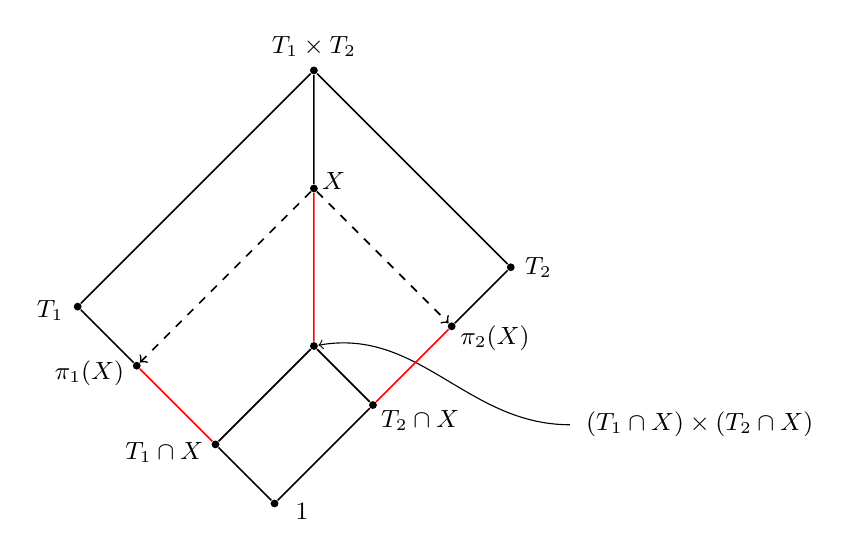
\begin{tikzpicture}[scale=.5]
    \node (e) at (0,0) [fill,circle,inner sep=1pt] {};
    \draw[font=\small] (.7,-.2) node {$1$};
    \node (T1capX) at (-1.5,1.5) [fill,circle,inner sep=1pt] {};
    \draw[font=\small] (-2.8,1.3) node {$T_1\cap X$};
    \node (T2capX) at (2.5,2.5) [fill,circle,inner sep=1pt] {};
    \draw[font=\small] (3.7,2.1) node {$T_2\cap X$};
    \node (pi1) at (-3.5,3.5) [fill,circle,inner sep=1pt] {};
    \draw[font=\small] (-4.7,3.3) node {$\pi_1(X)$};
    \node (pi2) at (4.5,4.5) [fill,circle,inner sep=1pt] {};
    \draw[font=\small] (5.6,4.2) node {$\pi_2(X)$};
    \node (Y) at (1,4) [fill,circle,inner sep=1pt] {};
    \draw[->] (7.5,2) to [out=180,in=10] (Y);
    \draw[font=\small] (10.8,2) node {$(T_1\cap X)\times (T_2 \cap X)$};

    \node (X) at (1,8) [fill,circle,inner sep=1pt] {};
    \draw[font=\small] (1.5,8.2) node {$X$};
    \node (T1) at (-5,5) [fill,circle,inner sep=1pt] {};
    \draw[font=\small] (-5.7,4.9) node {$T_1$};
    \node (T2) at (6,6) [fill,circle,inner sep=1pt] {};
    \draw[font=\small] (6.7,6) node {$T_2$};
    \node (T1T2) at (1,11) [fill,circle,inner sep=1pt] {};
    \draw[font=\small] (1,11.6) node {$T_1\times T_2$};


    \draw[semithick]
    (T1T2) to (X)
    (e) to (T1capX) to (Y) to (T2capX) to (e)
    (pi1) to (T1) to (T1T2) to (T2) to (pi2);

    \draw[->, dashed, semithick]
    (X) to (pi1);

    \draw[->, dashed, semithick]
    (X) to (pi2);
    
    \draw[red, semithick]
    (T1capX) to (pi1)
    (T2capX) to (pi2)
    (Y) to (X);
  \end{tikzpicture}
  \caption{Illustrates Theorem~\ref{thm:1} in case $n=2$.  Solid lines
    represent subgroup relations. Intervals colored red are isomorphic. Dashed
    lines emphasize the fact that the projections, $\pi_1(X)$ and
    $\pi_2(X)$, are not generally subgroups of $X$.}  
  \label{fig:theorem}
\end{center}
\end{figure}

Recall, $X$ is a subdirect product of $T_1, \dots, T_n$ provided
 $X \leq \prod\limits_k T_k $ and the projections are onto: $\pi_i(X)= T_i$.  We
denote this situation by  
%$X \stackrel{_{ \mathrm{sd}}}{\hookrightarrow} \prod_i T_i$.
$X \stackrel{_{\mathrm{sd}}}{\leq} \prod T_k$.
%$X \leq_{\mathrm{sd}}\prod_i T_i$.
The following is a consequence of Theorem~\ref{thm:1}:
% and the CFSG theorem:\footnote{The classification of
%finite simple groups (which is a theorem) is called ``the CFSG theorem.''}
\begin{corollary}
  If $T$ is a finite nonabelian simple group and 
$X \stackrel{_{\mathrm{sd}}}{\leq} T^n$,
%$X \stackrel{_{ \mathrm{sd}}}{\hookrightarrow} T^n$,
  then $T \cong X/ (T^{n-1}\cap X)$.  Thus, there are (at least) $n$ distinct normal
  subgroups of $X$ (namely,  $\hat{T}\cap X$) with the property that the
  quotient group is isomorphic to $T$.  In case $n=2$, every subdirect product
  of $T^2$ is isomorphic to $T$.
\end{corollary}
%\noindent \underline{Proof:} (coming soon)


\subsection{O'Nan-Scott types in GAP}
\label{sec:prim-perm-groups}
\GAP\ contains a library of primitive permutation groups which includes the
following permutation groups up to permutation isomorphism (i.e., up to
conjugacy in the corresponding symmetric group):
\begin{itemize}
\item 
all primitive permutation groups of degree $< 2500$, calculated by Colva Roney-Dougal in~\cite{Roney-Dougal:2005}; in particular,
\item the primitive permutation groups up to degree 50, calculated by C. Sims,
\item the primitive groups with insoluble socles of degree $< 1000$ as calculated in~\cite{Dixon:1988},
\item the solvable (hence affine) primitive permutation groups of degree $< 256$ as calculated in~\cite{Short:1992},
\item some insolvable affine primitive permutation groups of degree $< 256$ as calculated in~\cite{Theissen:1997}.
\item The solvable primitive groups of degree up to 999 as calculated in~\cite{Eick:2002}.
\item The primitive groups of affine type of degree up to 999 as calculated in~\cite{Roney-Dougal:2003}.
\end{itemize}
%Not all groups are named, those which do have names use ATLAS notation. Not all names are necessary unique!
The list given in~\cite{Roney-Dougal:2005} is believed to be complete,
correcting various omissions in~\cite{Dixon:1988}, \cite{Short:1992},
and~\cite{Theissen:1997}.  (The latest version of \GAP, version 4.5, is still in
beta-testing, but we expect it will incorporate the results
of Coutts, Quick, and Roney-dougal~\cite{Coutts_theprimitive} cataloging all
primitive groups of degree $< 4096$.)

%% Section 41.1 of the \gap\ manual covers primitive permutation groups.  Here are some
%% points that are important for our work.
\begin{itemize}
\item 
{\tt ONanScottType( $G$ )}
returns the type of a primitive permutation group $G$, according to the O'Nan-Scott classification. The
labeling of the different types is not consistent in the literature, and
\gap\ uses the following:
\begin{itemize}
\item 1 Affine.
\item 2 Almost simple.
\item 3a Diagonal, Socle consists of two normal subgroups.
\item 3b Diagonal, Socle is minimal normal.
\item 4a Product action with the first factor primitive of type 3a.
\item 4b Product action with the first factor primitive of type 3b.
\item 4c Product action with the first factor primitive of type 2.
\item 5 Twisted wreath product.
\end{itemize}
As it can contain letters, the type is returned as a string.
If $G$ is not a permutation group or does not act primitively on the points moved by it, the result is undefined.
Some examples of primitive permutation groups of relatively
small degree that are of types 2, 3a, 3b, and 4c are given below in Section~\ref{sec:examples-onan-scott}.
(Note, that for groups of degree up to 2499, O'Nan-Scott types 4a, 4b and 5
cannot occur.)


\item {\tt SocleTypePrimitiveGroup( $G$ )}
returns the socle type of a primitive permutation group. The socle of a primitive group is the direct product
of isomorphic simple groups, therefore the type is indicated by a record with
components {\tt series, parameter} 
(both as described under IsomorphismTypeInfoFiniteSimpleGroup, see below) and width for the
number of direct factors.
If $G$ does not have a faithful primitive action, the result is undefined.

\item\protect\footnotemark
\footnotetext{See Section 37.15 of the \gap\ manual.}
{\tt IsomorphismTypeInfoFiniteSimpleGroup( $G$ )}
For a finite simple group $G$, IsomorphismTypeInfoFiniteSimpleGroup returns a record with components
series, name and possibly parameter, describing the isomorphism type of $G$. The component name is a
string that gives name(s) for $G$, and series is a string that describes the following series.
(If different characterizations of $G$ are possible only one is given by series and parameter, while name may
give several names.)
{\footnotesize
\begin{itemize}
\item 
``A'' Alternating groups, parameter gives the natural degree.
\item 
``L'' Linear groups (Chevalley type A), parameter list [n,q] indicates L(n, q).
\item 
``2A'' Twisted Chevalley type 2 A, parameter list [n,q] indicates 2 A(n, q).
\item 
``B'' Chevalley type B, parameter list [n,q] indicates B (n, q).
\item 
``2B'' Twisted Chevalley type 2 B, parameter q indicates 2 B (2, q).
\item 
``C'' Chevalley type C, parameter list [n,q] indicates C (n, q).
\item 
``D'' Chevalley type D, parameter list [n,q] indicates D(n, q).
\item 
``2D'' Twisted Chevalley type 2 D, parameter list [n,q] indicates 2 D(n, q).
\item 
``3D'' Twisted Chevalley type 3 D, parameter q indicates 3 D(4, q).
\item 
``E'' Exceptional Chevalley type E, parameter list [n,q] indicates En (q). \\The value of n is 6, 7 or 8.
\item 
``2E'' Twisted exceptional Chevalley type E6, parameter q indicates 2 E6 (q).
\item 
``F'' Exceptional Chevalley type F , parameter q indicates F (4, q).
\item 
``2F'' Twisted exceptional Chevalley type 2 F (Ree groups), parameter q indicates 2 F (4, q).
\item 
``G'' Exceptional Chevalley type G, parameter q indicates G(2, q).
\item 
``2G'' Twisted exceptional Chevalley type 2 G (Ree groups), parameter q indicates 2 G(2, q).
\item 
``Spor'' Sporadic groups, name gives the name.
\item 
``Z'' Cyclic groups of prime size, parameter gives the size.
\end{itemize}
}
An equal sign in the name denotes different naming schemes for the same group, a tilde sign abstract
isomorphisms between groups constructed in a different way.

\end{itemize}


\newpage
\subsection{Examples of O'Nan-Scott types}
\label{sec:examples-onan-scott}
As noted in Section \ref{sec:prim-perm-groups}, the \GAP\ command {\tt ONanScottType( $G$ )}
returns the type of a primitive permutation group $G$, according to the
O'Nan-Scott classification described in
Section~\ref{sec:onan-scott-theorem}. 

In the tables below we give some examples of primitive permutation groups of relatively
small degree that are of types 2, 3a, 3b, and 4c.
(Note, that for groups of degree up to 2499, O'Nan-Scott types 4a, 4b and 5
cannot occur.)


{\small
  \begin{tabular}{r|l|l}
  \multicolumn{3}{c}{Type 2. \emph{Almost Simple Groups}}\\\toprule
  & & GAP Index \\
    Order & Name & {\tt PrimitiveGroup(i,j)} \\
%    $|G|$ & Name & GAP index \\
\midrule
 60 & $A_5$ & (5,4), (6,1), (10,1) \\
 120 & $S_5$ & (5,5), (6,2), (10,2) \\
 168 & $\PSL(3,2)$ & (7,5), (8,4) \\
 336 & $\PSL(3,2) \rtimes C_2$ & (8,5) \\
 360 & $A_6$ & (15,2), (6,3), (10,3) \\
 504 & $\PSL(2,8)$ & (9,8) \\
 660 & $\PSL(2,11)$ & (11,5), (12,3) \\
 720 & $S_6$ & (6,4), (10,5), (15,3) \\
 720 & $A_6 \rtimes C_2$ & (10,4) \\
 720 & $A_6 . C_2$ & (10,6) \\
 1,092 & $\PSL(2,13)$ & (14,1) \\
 1,320 & $\PSL(2,11) \rtimes C_2$ & (12,4) \\
 1,440 & $(A_6 . C_2) \rtimes C_2$ & (10,7) \\
 1,512 & $\PSL(2,8) \rtimes C3$ & (9,9) \\
 2,184 & $\PSL(2,13) \rtimes C_2$ & (14,2) \\
 2,448 & $\PSL(2,17)$ & (18,1) \\
 2,520 & $A_7$ & (7,6), (15,1) \\
 3,420 & $\PSL(2,19)$ & (20,1) \\
 4,080 & $\PSL(2,16)$ & (17,6) \\
 4,896 & $\PSL(2,17) \rtimes C_2$ & (18,2) \\
 5,040 & $S_7$ & (7,7) \\
 5,616 & $\PSL(3,3)$ & (13,7) \\
 6,840 & $\PSL(2,19) \rtimes C_2$ & (20,2) \\
 7,920 & $M_{11}$ & (11,6) \\
 7,920 & $M_{11}$ & (12,1) \\
 8,160 & $\PSL(2,16) \rtimes C_2$ & (17,7) \\
 16,320 & $\PSL(2,16) \rtimes C4$ & (17,8)\\
 20,160 & $A_8$ & (8,6), (15,4)  \\
 40,320 & $S_8$ & (8,7) \\
 95,040 & $M_{12}$ & (12,2) \\
 181,440 & $A_9$ & (9,10) \\
 362,880 & $S_9$ & (9,11) \\
 1,814,400 & $A_{10}$ & (10,8) \\
 3,628,800 & $S_{10}$ & (10,9) \\
 19,958,400 & $A_{11}$ & (11,7) \\
 39,916,800 & $S_{11}$ & (11,8)\\
 %% & $\vdots$  &  \\
 %% $n!/2$ & $A_{n}$ & $(n,i)$ \\
 %% $n!$ & $S_{n}$ & $(n,i+1)$\\
\end{tabular}




%% # 3a Diagonal, Socle consists of two normal subgroups.
  \begin{tabular}{r|l|l}
  \multicolumn{3}{c}{Type 3a. \emph{Diagonal, socle consists of two normal subgroups.}}\\\toprule
    Order & Name & GAP index \\
\midrule
 3,600 & $(A_5 \times A_5)$ &(60,1) \\
 7,200 & $(A_5 \times A_5) \rtimes C_2$ & (60,2) \\
 28,224 & $\PSL(3,2) \times \PSL(3,2)$ & (168,1) \\
 56,448 & $(\PSL(3,2) \times \PSL(3,2)) \rtimes C_2$ & (168,2) \\
 129,600 & $A_6 \times A_6$ & (360,1) \\
 259,200 & $(A_6 \times A_6) \rtimes C_2$ & (360,2) \\
 259,200 & $(A_6 \times A_6) \rtimes C_2$ & (360,3)\\
\end{tabular}

\vskip1cm

%% # 3b Diagonal, Socle is minimal normal.
  \begin{tabular}{r|l|l}
  \multicolumn{3}{c}{Type 3b. \emph{Diagonal, socle is minimal normal.}}\\\toprule
    Order & Name & GAP index \\
\midrule
 7,200 & $(A_5 \times A_5) \rtimes C_2$ & (60,3) \\
 7,200 & $(A_5 \times A_5) \rtimes C_2$ & (60,4) \\
 14,400 & $((A_5 \times A_5) \rtimes C_2) \rtimes C_2)$ & (60,5) \\
 56,448 & $(\PSL(3,2) \times \PSL(3,2)) \rtimes C_2$ & (168,3) \\
 56,448 & $(\PSL(3,2) \times \PSL(3,2)) \rtimes C_2$ & (168,4) \\
 112,896 & $((\PSL(3,2) \times \PSL(3,2)) \rtimes C_2) \rtimes C_2$ & (168,5) \\
 259,200 & $(A_6 \times A_6) \rtimes C_2$ & (360,5) \\
 259,200 & $(A_6 \times A_6) \rtimes C_2$ & (360,6)\\
\end{tabular}

\vskip1cm

%% # 4c Product action with the first factor primitive of type 2.
  \begin{tabular}{r|l|l}
  \multicolumn{3}{c}{Type 4c. \emph{Product action, first factor primitive type 2.}}\\\toprule
    Order & Name & GAP index \\
\midrule
 7,200 & $(A_5 \times A_5) \rtimes C_2$ & (25,23) \\
 14,400 & $((A_5 \times A_5) \rtimes C_2) \rtimes C_2$ & (25,24) \\
 14,400 & $(A_5 \times A_5) \rtimes C_4$ & (25,25) \\
 28,800 & $(S_5 \times S_5) \rtimes C_2$ & (25,26) \\
 259,200 & $(A_6 \times A_6) \rtimes C_2$ & (36,13) \\
 518,400 & $((A_6 \times A_6) \rtimes C_2) \rtimes C_2$ & (36,14) \\
 518,400 & $(A_6 \times A_6) \rtimes C_4$ & (36,15)\\
\end{tabular}
%% # 4a Product action with the first factor primitive of type 3a.
%% # 4b Product action with the first factor primitive of type 3b.
%% # 5 Twisted wreath product.
}


%% \midrule
%%  60 & $A_5$ & (5,4), (6,1), (10,1) \\
%%  120 & $S_5$ & (5,5), (6,2), (10,2) \\
%%  120 & $S_5$ & 
%%  168 & $\PSL(3,2)$ & (7,5) \\
%%  168 & $\PSL(3,2)$ & (8,4) \\
%%  360 & $A_6$ & (15,2) \\
%%  336 & $\PSL(3,2) : C_2$ & (8,5) \\
%%  360 & $A_6$ & (6,3) \\
%%  360 & $A_6$ & (10,3) \\
%%  504 & $\PSL(2,8)$ & (9,8) \\
%%  660 & $\PSL(2,11)$ & (11,5) \\
%%  660 & $\PSL(2,11)$ & (12,3) \\
%%  720 & $S_6$ & (6,4) \\
%%  720 & $A_6 : C_2$ & (10,4) \\
%%  720 & $S_6$ & (10,5) \\
%%  720 & $A_6 . C_2$ & (10,6) \\
%%  720 & $S_6$ & (15,3) \\
%%  1092 & $\PSL(2,13)$ & (14,1) \\
%%  1320 & $\PSL(2,11) : C_2$ & (12,4) \\
%%  1440 & $(A_6 . C_2) : C_2$ & (10,7) \\
%%  1512 & $\PSL(2,8) : C3$ & (9,9) \\
%%  2184 & $\PSL(2,13) : C_2$ & (14,2) \\
%%  2448 & $\PSL(2,17)$ & (18,1) \\
%%  2520 & $A_7$ & (7,6) \\
%%  2520 & $A_7$ & (15,1) \\
%%  3420 & $\PSL(2,19)$ & (20,1) \\
%%  4080 & $\PSL(2,16)$ & (17,6) \\
%%  4896 & $\PSL(2,17) : C_2$ & (18,2) \\
%%  5040 & $S_7$ & (7,7) \\
%%  5616 & $\PSL(3,3)$ & (13,7) \\
%%  6840 & $\PSL(2,19) : C_2$ & (20,2) \\
%%  7920 & $M_{11}$ & (11,6) \\
%%  7920 & $M_{11}$ & (12,1) \\
%%  8160 & $\PSL(2,16) : C_2$ & (17,7) \\
%%  16320 & $\PSL(2,16) : C4$ & (17,8)
%%  20160 & $A_8$ & (8,6), (15,4)  \\
%%  40320 & $S_8$ & (8,7) \\
%%  95040 & $M_{12}$ & (12,2) \\
%%  181440 & $A_9$ & (9,10) \\
%%  362880 & $S_9$ & (9,11) \\
%%  1814400 & $A_{10}$ & (10,8) \\
%%  3628800 & $S_{10}$ & (10,9) \\
%%  & $\vdots$  &  \\
%%  $n!/2$ & $A_{n}$ & $(n,i)$ \\
%%  $n!$ & $S_{n}$ & $(n,i+1)$\\
%% \end{tabular}


%%   \begin{tabular}{r|l|l}
%%   \multicolumn{3}{c}{Type 2. \emph{Almost Simple Groups}}\\\toprule
%%     Order & Name & GAP index \\
%% \midrule
%%  20160 & $A_8$ & (8,6) \\
%%  20160 & $A_8$ & (15,4) \\
%%  40320 & $S_8$ & (8,7) \\
%%  95040 & $M_{12}$ & (12,2) \\
%%  181440 & $A_9$ & (9,10) \\
%%  362880 & $S_9$ & (9,11) \\
%%  1814400 & $A_{10}$ & (10,8) \\
%%  3628800 & $S_{10}$ & (10,9) \\
%%  & $\vdots$  &  \\
%%  $n!/2$ & $A_{n}$ & $(n,i)$ \\
%%  $n!$ & $S_{n}$ & $(n,i+1)$\\
%% \end{tabular}
 %% 239500800 & $A_{12}$ & (12,5) \\
 %% 479001600 & $S_{12}$ & (12,6) \\
 %% 3113510400 & $A_{13}$ & (13,8) \\
 %% 6227020800 & $S_{13}$ & (13,9) \\
 %% 43589145600 & $A_{14}$ & (14,3) \\
 %% 87178291200 & $S_{14}$ & (14,4) \\
 %% 653837184000 & $A_{15}$ & (15,5) \\
 %% 1307674368000 & $S_{15}$ & (15,6) \\
 %% 10461394944000 & $A_{16}$ & (16,21) \\
 %% 20922789888000 & $S_{16}$ & (16,22) \\
 %% 177843714048000 & $A_{17}$ & (17,9) \\
 %% 355687428096000 & $S_{17}$ & (17,10) \\
 %% 3201186852864000 & $A_{18}$ & (18,3) \\
 %% 6402373705728000 & $S_{18}$ & (18,4) \\
 %% 60822550204416000 & $A_{19}$ & (19,7) \\
 %% 121645100408832000 & $S_{19}$ & (19,8) \\
 %% 1216451004088320000 & $A_{20}$ & (20,3) \\
 %% 2432902008176640000 & $S_{20}$ & (20,4)


\newpage
\part*{GAP Supplement}

\newpage
\section{Preliminaries: a few basic commands}
\begin{enumerate}[a.]
\item {\bf Help.}  A convenient way of reading the documentation at the gap prompt is
 with the {\tt ?} symbol, as in:
{\codesize
\begin{verbatim}
?tutorial:a first session with gap
\end{verbatim}}
\noindent This starts the basic \gap\ tutorial.  After reading the first page,
you can move to the next page by entering {\tt ?>}, and the previous page with
{\tt ?<}.  

As another example, if you want to learn about commands involving, say,
the centralizer, just enter the command
{\tt ?centralizer} for a list of related help topics.

\item {\bf Comments} 
in \gap\ begin with the sharp character {\tt \#}.  The whole comment, including
{\tt \#} and the newline character, is treated as a single whitespace. 
%Inside a string, the comment character {\tt \#} loses its role and is just
%an ordinary character.

\item {\bf Functions.} You can define a function in a ${\tt .gap}$ file or ``in-line'' as follows:
{\codesize
\begin{verbatim}
 cubed := x -> x^3;
\end{verbatim}}
\noindent Then {\tt cubed(5)} returns 125.

\item 
\gap\ composes permutations left-to-right.  
That is, \verb|(1,2,4)*(1,2)| gives \verb|(2,4)|;\\
\emph{not} right-to-left; that is, $(1,2,4)(1,2) \neq (1,4)$.

\item
The carrot operator \verb|^| is used to determine the image of a point under a
permutation and to conjugate one permutation by another. 
e.g.~\verb|(1,2,3)^-1| gives \verb|(1,3,2)|, \verb|2^(1,2,3)| gives 3, and
\verb|(1,2,3)^(1,2)| gives \verb|(1,3,2)|.
That is (for the last one), $(1,2,3)^{(1,2)} = (1,2)(1,2,3)(1,2) = (1,3,2)$.
\item
The preimage of a point $i$ under a permutation $p$ is given by $i/p$.  For example,
\verb|2/(1,2,3)| gives 1, and, since $(1,2,4)(1,2) = (2,4)$,
\verb|3/((1,2,4)(1,2))| gives 3, and \verb|2/((1,2,4)(1,2))| gives 4.
\item 
You can get an overview of all \gap\ variables with the command {\tt NamesGVars();} and
you can see the user-defined variables of the current session using 
{\tt NamesUserGVars();}.
The name of every global variable in the \gap\ library starts with a capital letter, so you
should start user-defined variable names with a lower case letter (or a number).
\end{enumerate}

\newpage 

\section{Some important groups\protect\footnotemark}  
\footnotetext{See also the \gap\ Manual~\cite{gapmanual}, Chapter 48 ``Group Libraries.''}
There are several infinite families of groups which are parametrized by numbers. \gap\
provides various functions to construct these groups. The functions always permit
(but do not require) one to indicate a 
filter, for example {\tt IsPermGroup, IsMatrixGroup} or {\tt IsPcGroup}, in which the
group shall be constructed. 
There always is a default filter corresponding to a ``natural'' way to describe the
group in question. Note that not every group can be constructed in every filter,
there may be theoretical restrictions ({\tt IsPcGroup} only works for solvable
groups) or methods may be available only for a few filters. 
Certain filters may admit additional hints. For example, groups constructed in
{\tt IsMatrixGroup} may be constructed over a specified field, which can be given as
second argument of the function that constructs the group; The default field is
{\tt Rationals}.
\begin{itemize}
\item {\tt TrivialGroup( [filt] )}\\[2pt] 
constructs a trivial group in the category given by the filter {\tt filt}. If {\tt filt} is not given it defaults to
{\tt IsPcGroup}. %For example,
{\codesize
\begin{verbatim}
gap> TrivialGroup();
<pc group of size 1 with 0 generators>
gap> TrivialGroup( IsPermGroup );    # returns Group(())
\end{verbatim}}
\noindent CAUTION: if you want to test whether a certain subgroup $H \leq G$ is the
identity of $G$, you can't simply type {\tt H=Group(())} or {\tt H=TrivialGroup()}.  
Instead, define the trivial subgroup of $G$ with {\tt e:=Group([Identity(G)])}.  Then
{\tt H=e} tests whether $H$ is trivial.

\item {\tt CyclicGroup( [filt, ] n )}\\[2pt] 
constructs the cyclic group of size n in the category {\tt filt}. 
If {\tt filt} is not given it defaults to {\tt IsPcGroup}.
%For example, 
{\codesize
\begin{verbatim}
gap> CyclicGroup(12);
<pc group of size 12 with 3 generators>
gap> CyclicGroup(IsPermGroup,12);
Group([ (1,2,3,4,5,6,7,8,9,10,11,12) ])
gap> matgrp1:= CyclicGroup( IsMatrixGroup, 12 );
<matrix group of size 12 with 1 generators>
gap> FieldOfMatrixGroup( matgrp1 );
Rationals
gap> matgrp2:= CyclicGroup( IsMatrixGroup, GF(2), 12 );
<matrix group of size 12 with 1 generators>
gap> FieldOfMatrixGroup( matgrp2 );
GF(2)
\end{verbatim}}
\item {\tt AbelianGroup( [filt, ] i )}\\[2pt] 
constructs an abelian group in the category {\tt filt} which is
of isomorphism type 
\[
\Z_{\mbox{i}[1]} \oplus \Z_{\mbox{i}[2]} \oplus \cdots \oplus \Z_{\mbox{i}[n]}.
\]
Here {\tt i} must be a list of positive integers. If {\tt filt} is not given it
defaults to {\tt IsPcGroup}. 
The generators of the group returned corresponding to the integers in {\tt i}.  %For example,
{\codesize
\begin{verbatim}
gap> AbelianGroup([1,2,3]);
<pc group of size 6 with 3 generators>
\end{verbatim}}
\item {\tt ElementaryAbelianGroup( [filt, ] n )}\\[2pt] 
constructs the elementary abelian group of size n in the category given by the filter
{\tt filt}. If {\tt filt} is not given it defaults to {\tt IsPcGroup}.
%For example,
{\codesize
\begin{verbatim}
gap> ElementaryAbelianGroup(8192);
<pc group of size 8192 with 13 generators>
\end{verbatim}}
\item {\tt DihedralGroup( [filt, ] n )}\\[2pt] 
constructs the dihedral group of size n in the category given by the filter
{\tt filt}. If {\tt filt} is not given it defaults to {\tt IsPcGroup}.
%For example,
{\codesize
\begin{verbatim}
gap> DihedralGroup(10);
<pc group of size 10 with 2 generators>
\end{verbatim}}
% \item {\tt ExtraspecialGroup( [filt, ] ord, exp )}\\[2pt] 
% Let {\tt ord} be of the form $p^{2n+1}$, for a prime integer $p$ and a positive integer $n$. 
% {\tt ExtraspecialGroup} returns the extraspecial group of order {\tt ord} that is
% determined by {\tt exp}, in the category given by the filter {\tt filt}. 
% If $p$ is odd then admissible values of {\tt exp} are the exponent of the group
% (either $p$ or $p^2$) or one of 
% {\tt '+', "+", '-',} or {\tt "-"}. For $p = 2$, only the above plus or minus signs are admissible.
% If {\tt filt} is not given it defaults to {\tt IsPcGroup}.
% \begin{verbatim}
% gap> ExtraspecialGroup( 27, 3 );
% <pc group of size 27 with 3 generators>
% gap> ExtraspecialGroup( 27, '+' );
% <pc group of size 27 with 3 generators>
% gap> ExtraspecialGroup( 8, "-" );
% <pc group of size 8 with 3 generators>
% \end{verbatim}
\item {\tt AlternatingGroup( [filt, ] deg )}
\item {\tt AlternatingGroup( [filt, ] dom )}\\[2pt] 
constructs the alternating group of degree {\tt deg} in the category given by the
filter {\tt filt}. 
If {\tt filt} is not given it defaults to {\tt IsPermGroup}.
In the second version, the function constructs the alternating group on the points
given in the set {\tt dom} which must be a set of positive integers.
{\codesize
\begin{verbatim}
gap> AlternatingGroup(5);
Alt( [ 1 .. 5 ] )
\end{verbatim}}
\item {\tt SymmetricGroup( [filt, ] deg )}
\item {\tt SymmetricGroup( [filt, ] dom )}\\[2pt] 
constructs the symmetric group of degree {\tt deg} in the category given by the
filter {\tt filt}. 
If {\tt filt} is not given it defaults to {\tt IsPermGroup}.
In the second version, the function constructs the symmetric group on the points
given in the set {\tt dom} which must be a set of positive integers.
{\codesize
\begin{verbatim}
gap> SymmetricGroup(10);
Sym( [ 1 .. 10 ] )
\end{verbatim}}
\end{itemize}

\newpage

\section{Factor groups\protect\footnotemark}  
\footnotetext{See also the \gap\ Manual~\cite{gapmanual}, Section 37.18.}
\begin{itemize}
\item {\tt NaturalHomomorphismByNormalSubgroup( G, N )}
\item {\tt NaturalHomomorphismByNormalSubgroupNC( G, N )}\\[2pt] 
returns a homomorphism from $G$ to another group whose kernel is $N$. \gap\ will try to select the image
group as to make computations in it as efficient as possible. As the factor group $G/N$ can be identified with
the image of $G$ this permits efficient computations in the factor group. The homomorphism returned is not
necessarily surjective, so {\tt ImagesSource} should be used instead of {\tt Range} to get a group isomorphic to the
factor group. The {\tt NC} variant does not check whether $N$ is normal in $G$.
\item {\tt FactorGroup( G, N )}, {\tt FactorGroupNC( G, N )}\\[2pt] 
%\item {\tt FactorGroupNC( G, N )}\\[2pt] 
returns the image of the {\tt NaturalHomomorphismByNormalSubgroup(G,N)}. The {\tt NC} version does not test
whether $N$ is normal in $G$.
{\codesize
\begin{verbatim}
gap> g:=Group((1,2,3,4),(1,2));;  n:=Subgroup(g,[(1,2)(3,4),(1,3)(2,4)]);;
gap> hom:=NaturalHomomorphismByNormalSubgroup(g,n);
[ (1,2,3,4), (1,2) ] -> [ f1*f2, f1 ]
gap> Size(ImagesSource(hom));  # returns 6
gap> FactorGroup(g,n);         # returns Group([ f1, f2 ])
\end{verbatim}}
\item {\tt CommutatorFactorGroup( G )}\\[2pt] 
computes the commutator factor group $G/G'$ of the group $G$.
{\codesize
\begin{verbatim}
gap> CommutatorFactorGroup(g);
Group([ f1 ])
\end{verbatim}}
\item {\tt MaximalAbelianQuotient( grp )}\\[2pt] 
returns an epimorphism from {\tt grp} onto the maximal abelian quotient of {\tt grp}. The kernel of this epimorphism
is the derived subgroup.
\item {\tt HasAbelianFactorGroup( G, N )}\\[2pt] 
tests whether $G/N$ is abelian (without explicitly constructing the factor group).
\item {\tt HasElementaryAbelianFactorGroup( G, N )}\\[2pt] 
tests whether $G/N$ is elementary abelian (without explicitly constructing the factor group).
{\codesize
\begin{verbatim}
gap> HasAbelianFactorGroup(g,n);                    # returns  false
gap> HasAbelianFactorGroup(DerivedSubgroup(g),n);   # returns  true
\end{verbatim}}
\item {\tt CentralizerModulo( G, N, x )}\\[2pt] 
computes the full preimage of the centralizer $C_{G/N} (\mathrm{x} \cdot N)$ in $G$ 
(without necessarily constructing the factor group).
{\codesize
\begin{verbatim}
gap> CentralizerModulo(g,n,(1,2));
Group([ (3,4), (1,3)(2,4), (1,4)(2,3) ])
\end{verbatim}}
\end{itemize}

\newpage

\section{Some important subgroups}
In the following, we refer to ``magmas'' which
  are more general than groups.  If you are not familiar with magmas, just substitute
  the word group for the word magma.
  \begin{itemize}
\item {\tt Normalizer( G, U )}
\item {\tt Normalizer( G, g )}\\[2pt]
Computes the normalizer $N_G(U)$, that is the stabilizer of $U$ under the conjugation
action of $G$. The second form computes $N_G(\langle g \rangle)$.
{\codesize
\begin{verbatim}
gap> Normalizer(g,Subgroup(g,[(1,2,3)]));  # returns Group([ (1,2,3), (2,3) ])
\end{verbatim}}
\item {\tt Centralizer( M, s )}
\item {\tt Centralizer( M, S )}\\[2pt]
For an element s of the magma M this operation returns the centralizer of s. 
This is the domain of those elements m in M that commute with s.
For a submagma S it returns the domain of those elements that commute with all elements s of S.
\item {\tt Center( M )}
Center returns the center of the magma M; i.e., the domain of those elements m in M that commute and
associate with all elements of M. 
For associative magmas we have that Center( M ) = Centralizer( M, M ).
The center of a magma is always commutative.

\item {\tt CommutatorSubgroup( G, H )}\\[2pt]
If $G$ and $H$ are two groups of elements in the same family, this operation returns the group generated
by all commutators $[g, h] = g h g^{-1} h^{-1}$ of elements $g\in G$ and $h\in H$; that is, the group
$\langle [g, h] \mid g \in G,  h \in H\rangle$. % For example,
{\codesize
\begin{verbatim}
gap> CommutatorSubgroup(Group((1,2,3),(1,2)),Group((2,3,4),(3,4)));
Group([ (1,4)(2,3), (1,3,4) ])
gap> Size(last);               # returns 12
\end{verbatim}}
\item {\tt DerivedSubgroup( G )}\\[2pt]
The derived subgroup $G'$ of $G$ is the subgroup generated by all commutators of pairs of elements of $G$. It
is normal in $G$ and the factor group $G/G'$ is the largest abelian factor group of $G$.
If $G/H$ is abelian, then $G' \leq H$.
\item {\tt Core( S, U )}\\[2pt]
If S and U are groups of elements in the same family, this operation returns the core
of U in S, that is the intersection of all S-conjugates of U.
%For example,
{\codesize
\begin{verbatim}
gap> g:=Group((1,2,3,4),(1,2));;
gap> Core(g,Subgroup(g,[(1,2,3,4)]));    # returns Group(())
\end{verbatim}}
\item {\tt PCore( G, p )}\\[2pt]
The p-core of G is the largest normal p-subgroup of G. It is the core of a p-Sylow
subgroup of G.
  \end{itemize}

%\subsection{Sets of Subgroups\protect\footnotemark}
%\footnotetext{{\it Ibid.}, sec.~37.19.}
\subsection{Sets of Subgroups}
\begin{itemize}
\item {\tt ConjugacyClassSubgroups( $G$, $U$ )}\\
generates the conjugacy class of subgroups of $G$ with representative $U$. This class
is an external set, so functions such as {\tt Representative}, (which returns $U$),
{\tt ActingDomain} (which returns $G$), {\tt StabilizerOfExternalSet} (which returns
the normalizer of $U$), and {\tt AsList} work for it. \\[4pt]
(The use of {\tt []} list access to select elements of the class is considered
obsolete and will be removed in future versions. Use {\tt ClassElementLattice} instead.)
{\codesize
\begin{verbatim}
gap> g:=Group((1,2,3,4),(1,2));;
gap> IsNaturalSymmetricGroup(g);   # returns true
gap> cl:=ConjugacyClassSubgroups( g, Subgroup(g,[(1,2)]) );
Group( [ (1,2) ] )^G
gap> Size(cl);                     # returns 6
gap> ClassElementLattice( cl, 4 ); # returns Group([ (2,3) ])
\end{verbatim}}

\item {\tt IsConjugacyClassSubgroupsRep( obj )}
\item {\tt IsConjugacyClassSubgroupsByStabilizerRep( obj )}\\
Is the representation \gap\ uses for conjugacy classes of subgroups. It can be used to check whether an
object is a class of subgroups. The second function {\tt ...ByStabilizerRep}
is, in addition, an external orbit by stabilizer and will compute its elements via a
transversal of the stabilizer. 

\item {\tt ConjugacyClassesSubgroups( $G$ )}\\
This attribute returns a list of all conjugacy classes of subgroups of the group
$G$. It also is applicable for lattices of subgroups. The order in which the classes
are listed depends on the method chosen by \gap. For each class of subgroups, a
representative can be accessed using {\tt Representative}.%\footnote{{\it Ibid.}, sec.~28.3.7.}
{\scriptsize
\begin{verbatim}
gap> ConjugacyClassesSubgroups( g );
[ Group( () )^G, Group( [ (1,3)(2,4) ] )^G, Group( [ (3,4) ] )^G,
Group( [ (2,4,3) ] )^G, Group( [ (1,4)(2,3), (1,3)(2,4) ] )^G,
Group( [ (1,2)(3,4), (3,4) ] )^G, Group( [ (1,2)(3,4), (1,3,2,4) ] )^G,
Group( [ (3,4), (2,4,3) ] )^G, Group( [ (1,3)(2,4), (1,4)(2,3), (1,2) ] )^G,
Group( [ (1,3)(2,4), (1,4)(2,3), (2,4,3) ] )^G,
Group( [ (1,3)(2,4), (1,4)(2,3), (2,4,3), (1,2) ] )^G ]
\end{verbatim}}

\item {\tt ConjugacyClassesMaximalSubgroups( $G$ )}\\
returns the conjugacy classes of maximal subgroups of $G$. Representatives of the
classes can be computed directly by {\tt MaximalSubgroupClassReps} (see next item).
{\codesize
\begin{verbatim}
gap> ConjugacyClassesMaximalSubgroups( g );
[ AlternatingGroup( [ 1 .. 4 ] )^G, Group( [ (1,2,3), (1,2) ] )^G,
Group( [ (1,2), (3,4), (1,3)(2,4) ] )^G ]
\end{verbatim}}

\item {\tt MaximalSubgroupClassReps( $G$ )}
returns a list of conjugacy representatives of the maximal subgroups of $G$.
{\codesize
\begin{verbatim}
gap> MaximalSubgroupClassReps( g );
[ Alt( [ 1 .. 4 ] ), Group([ (1,2,3), (1,2) ]),
Group([ (1,2), (3,4), (1,3)(2,4) ]) ]
\end{verbatim}}

\item {\tt MaximalSubgroups( $G$ )}\\
returns a list of all maximal subgroups of $G$. This may take up much space, therefore the command should
be avoided if possible (e.g., by using {\tt ConjugacyClassesMaximalSubgroups( $G$ )}
instead.)
{\codesize
\begin{verbatim}
gap> MaximalSubgroups( Group((1,2,3),(1,2)) );
[Group([ (1,2,3) ]), Group([ (2,3) ]), Group([ (1,2) ]), Group([ (1,3) ])]
\end{verbatim}}

\item {\tt NormalSubgroups( $G$ )}\\
returns a list of all normal subgroups of $G$.
{\codesize
\begin{verbatim}
gap> g := SymmetricGroup( 4 );;  NormalSubgroups( g );
[ Group(()), Group([ (1,4)(2,3), (1,3)(2,4) ]),
Group([ (2,4,3), (1,4)(2,3), (1,3)(2,4) ]), Sym( [ 1 .. 4 ] ) ]
\end{verbatim}}
%\noindent The algorithm used for the computation of normal subgroups of permutation groups and pc groups is
%described in [Hul98].

\item {\tt MaximalNormalSubgroups( $G$ )}\\
is a list containing those proper normal subgroups of the group $G$ that are maximal among the proper
normal subgroups.
{\codesize
\begin{verbatim}
    gap> MaximalNormalSubgroups( g );
    [ Group([ (2,4,3), (1,4)(2,3), (1,3)(2,4) ]) ]
\end{verbatim}}

\item {\tt MinimalNormalSubgroups( $G$ )}\\
  is a list containing those nontrivial normal subgroups of the group $G$ that
  are minimal among the nontrivial normal subgroups.
{\codesize
\begin{verbatim}
    gap> MinimalNormalSubgroups( g );  
    [ Group([ (1,4)(2,3), (1,3)(2,4) ]) ]
\end{verbatim}}
\end{itemize}
\subsectionspace

\subsection{Subgroup Lattice}
There is a very useful \gap\ package called \xgap\ which produces nice graphical
displays of subgroup lattices.  If you have \xgap\ installed
and running, at the command prompt you can try, for example:
{\codesize
\begin{verbatim}
gap> g := SymmetricGroup( 4 );;
gap> GraphicSubgroupLattice( g );
\end{verbatim}
}  
\begin{figure}[!hb]
    \vspace{-4cm}
    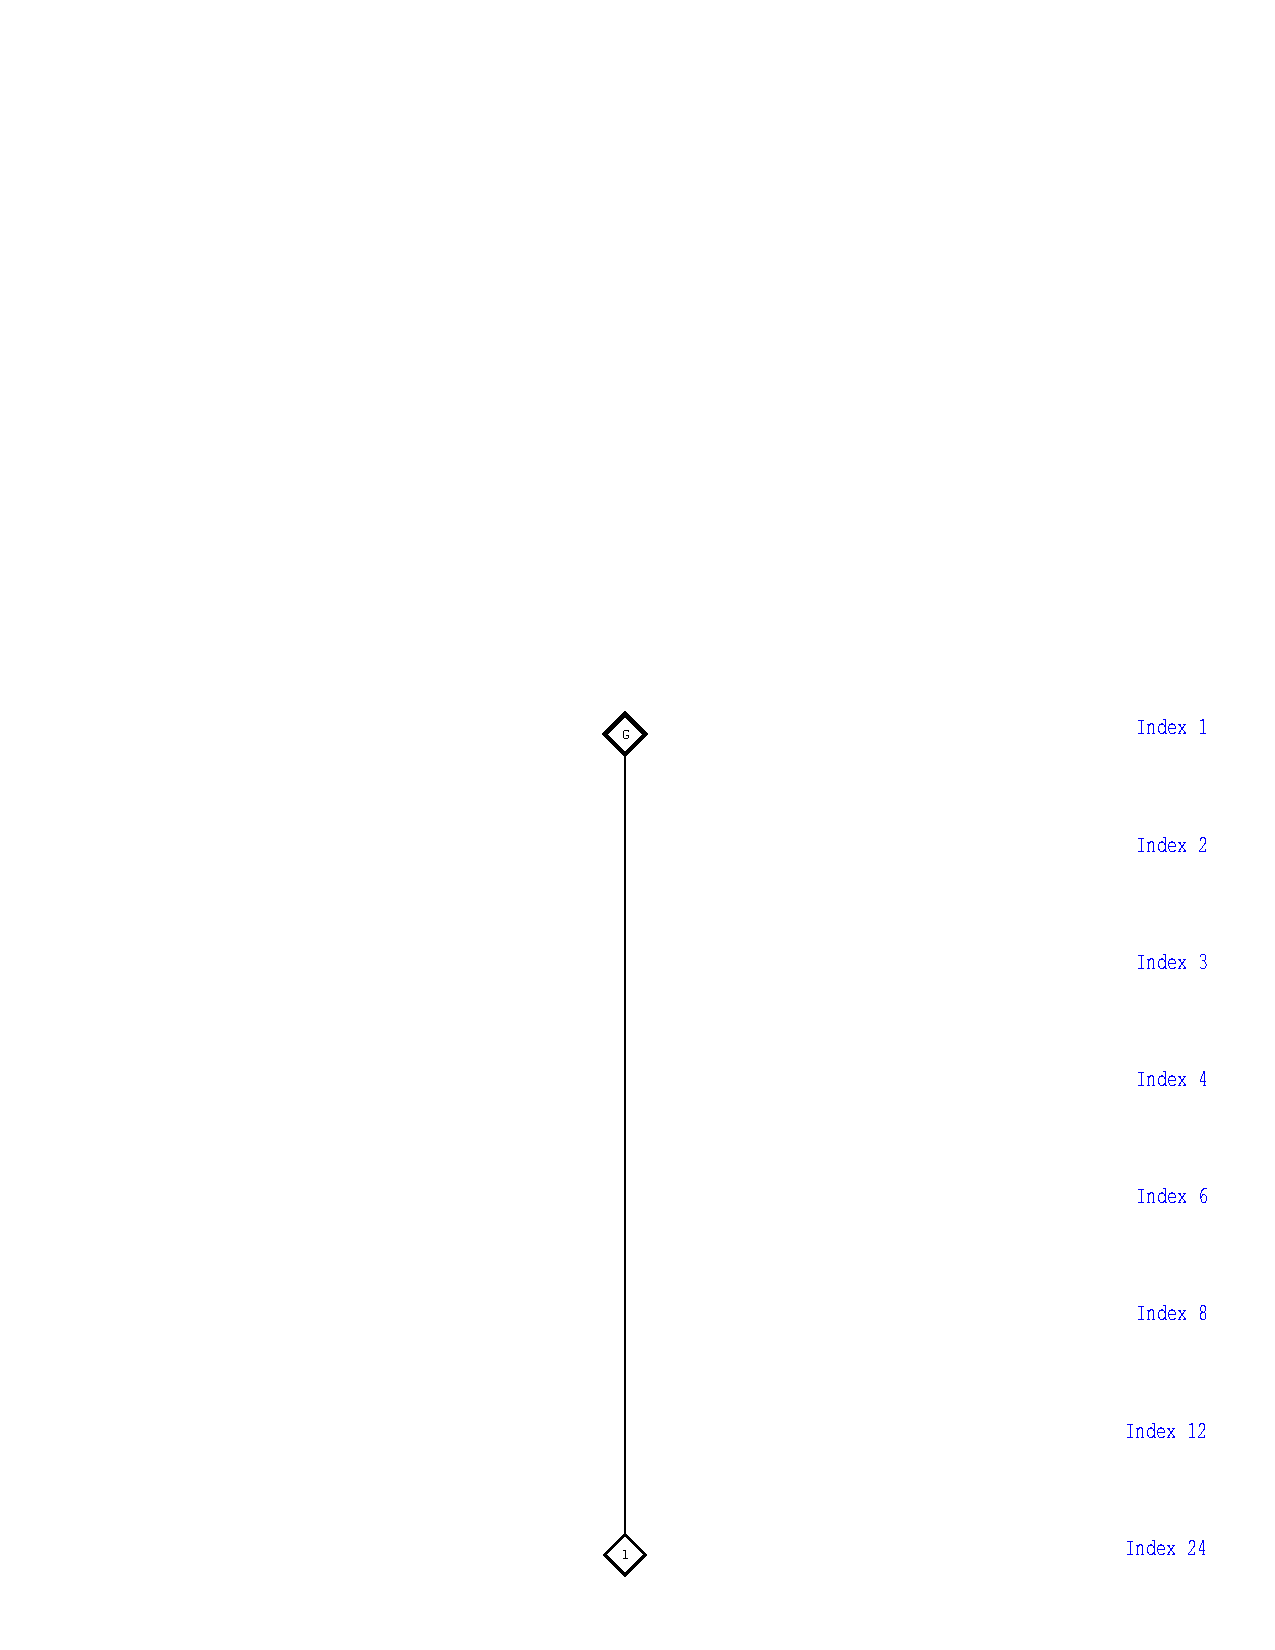
\includegraphics[height=10cm]{trivialS4.pdf}%
    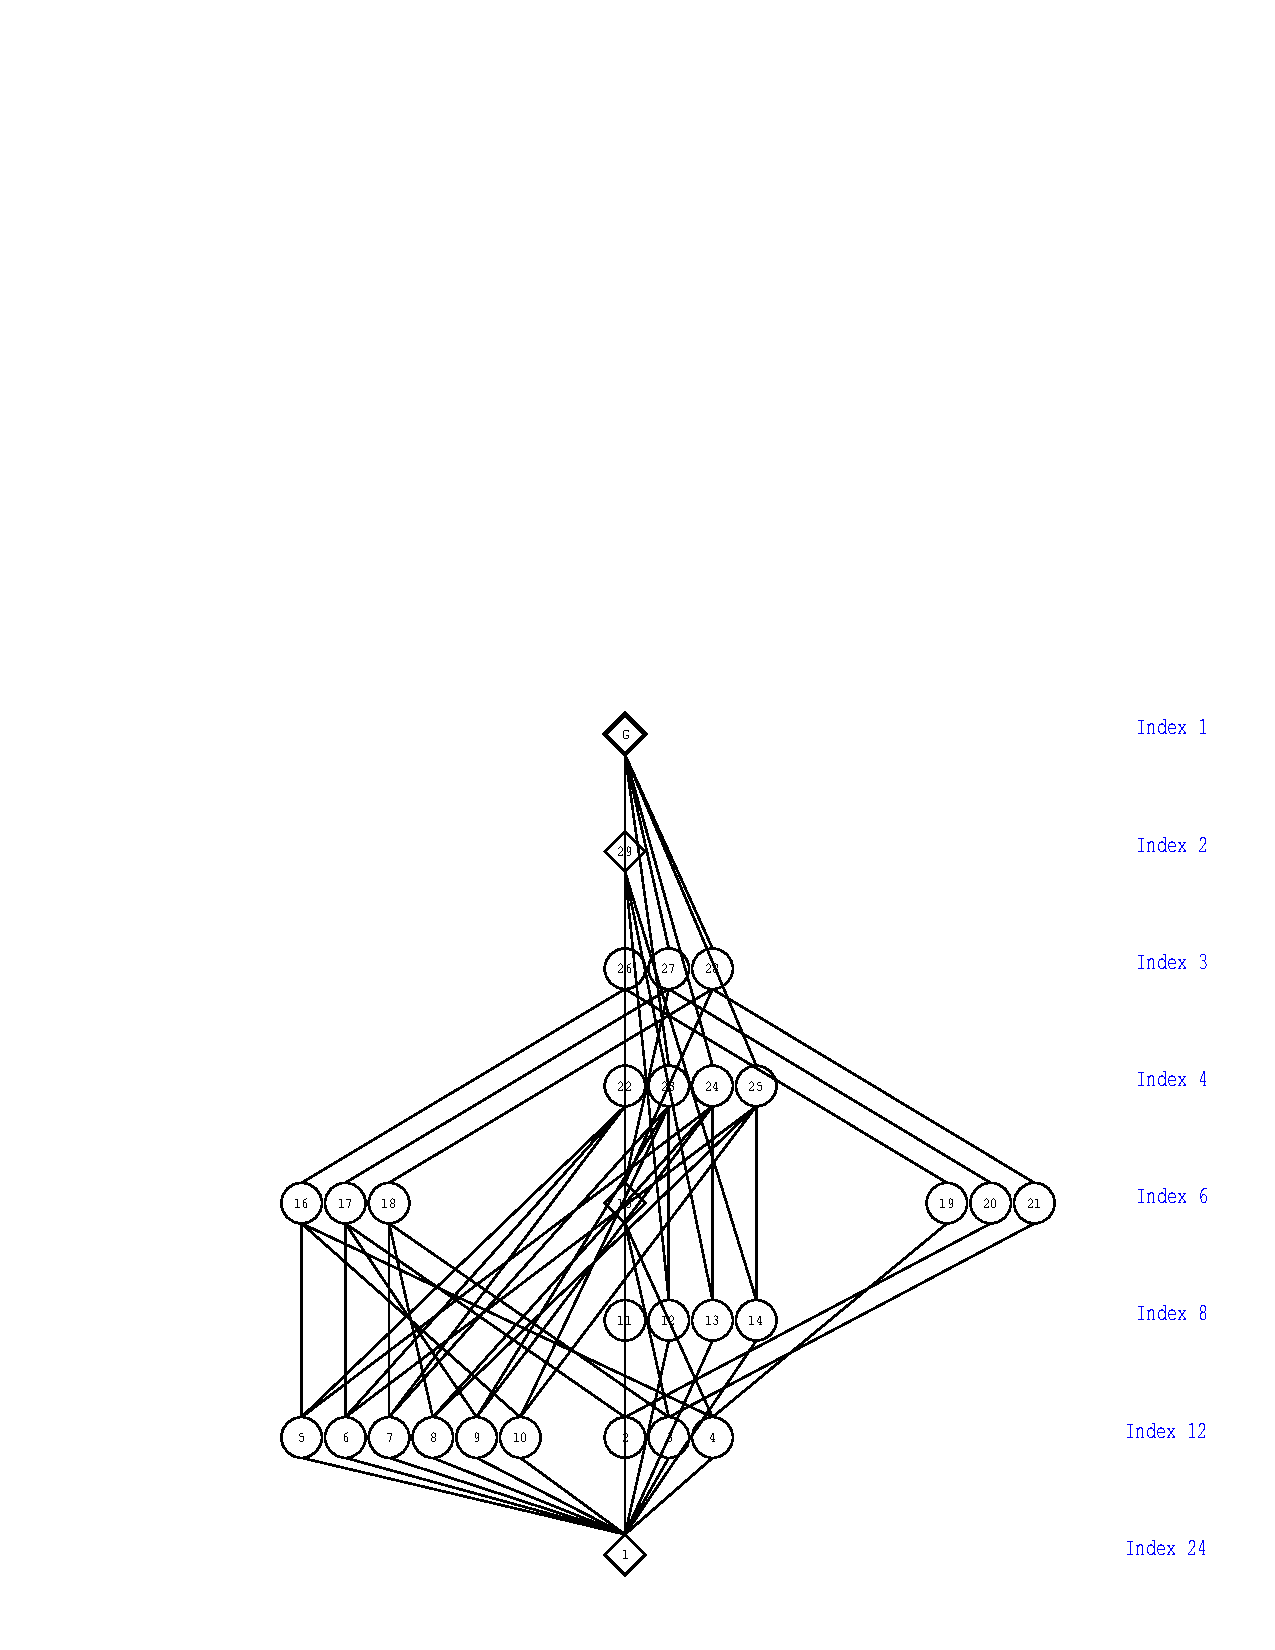
\includegraphics[height=10cm]{messyS4.pdf}%
    \caption{The subgroups $(e)$ and $S_4$ (left),
      and the full subgroup lattice $\Sub[S4]$ (right).}
    \label{fig:S4s}
\end{figure}
\begin{figure}[!h]
  \begin{center}
    \vspace{-4cm}
    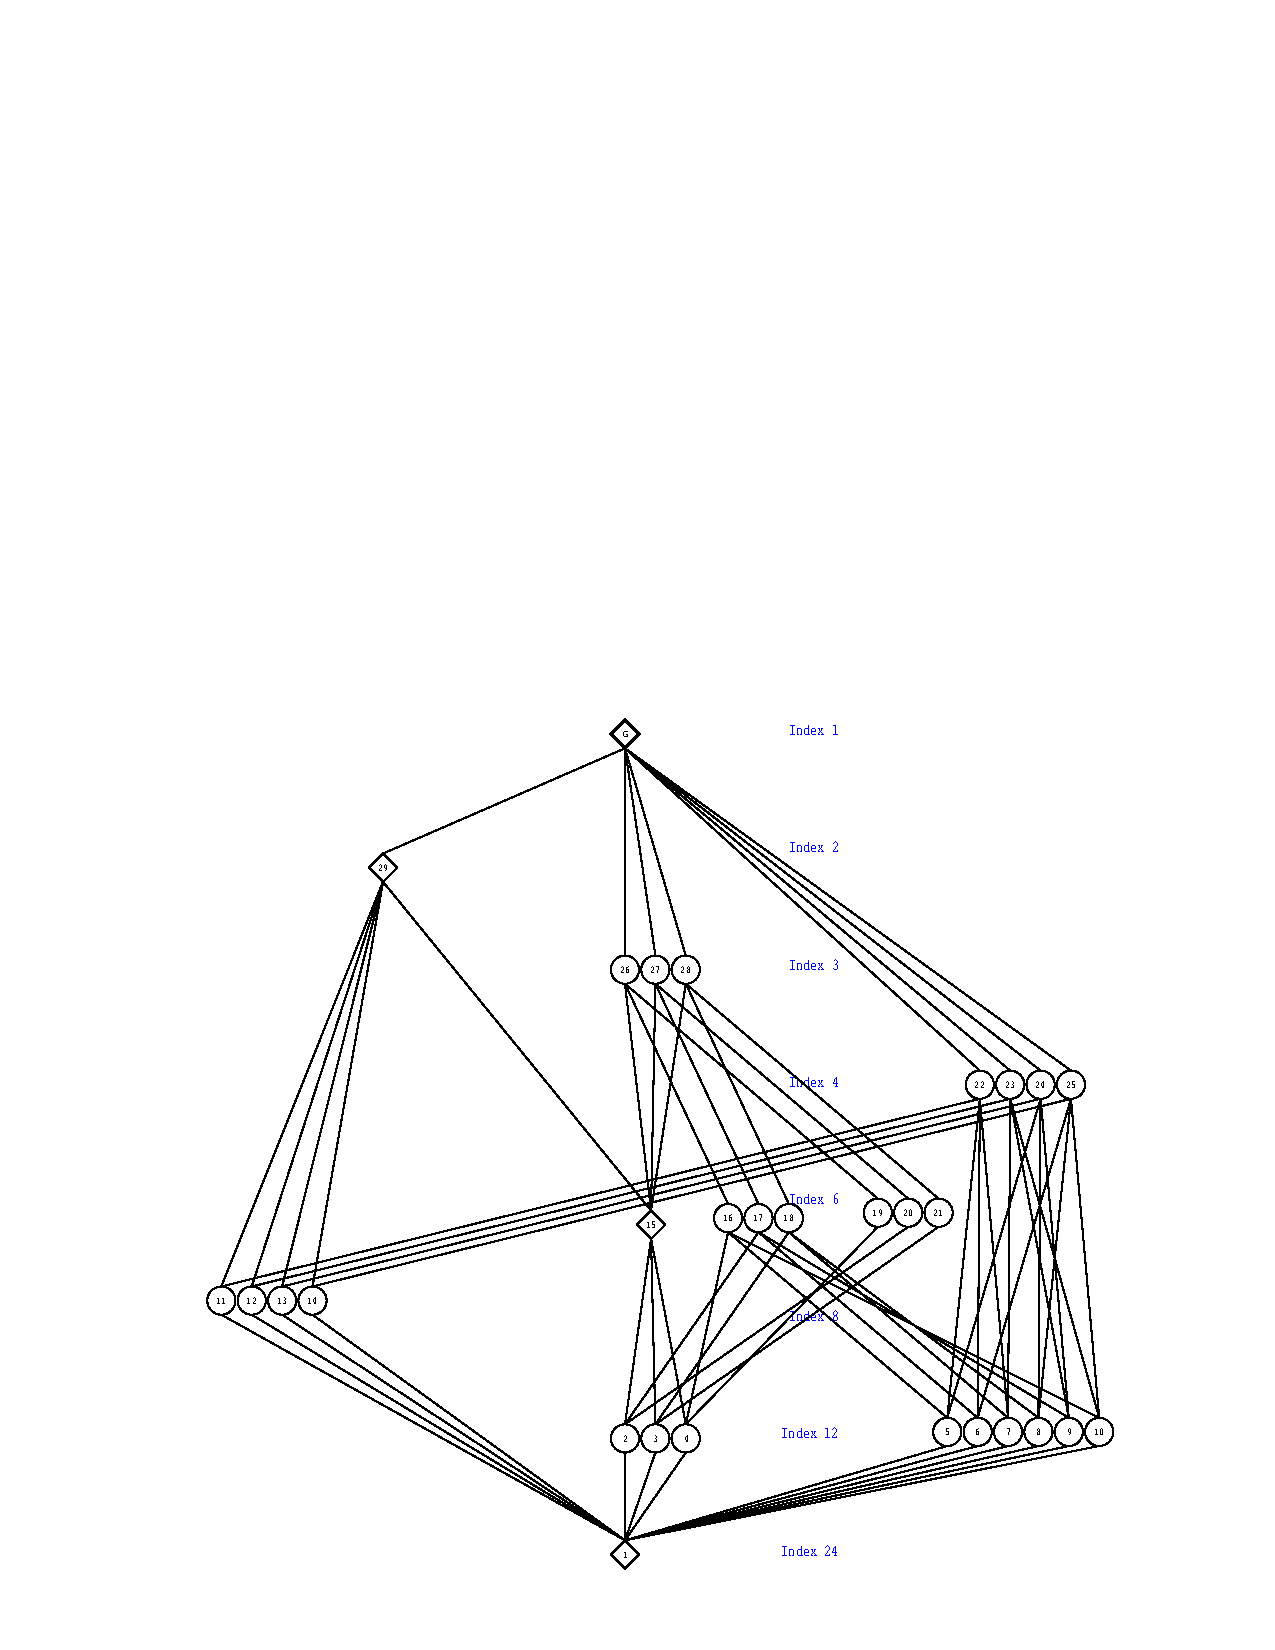
\includegraphics[height=12cm]{neatS4.pdf}%
    \caption{$\Sub[S4]$ as drawn by the \xgap\ program.}
    \label{fig:neatS4}
  \end{center}
\end{figure}
This opens a new \xgap\ graphics window showing just the two subgroups $(e)$ and
$S_4$ -- Figure~\ref{fig:S4s} (left).  In
the {\tt Subgroups} menu of this new window, select {\tt All Subgroups}.  This
fills in the subgroup lattice $\Sub[S_4]$ (in a rather messy way) -- Figure~\ref{fig:S4s}
(right).  You can then move the subgroups around to make it look nicer --
Figure~\ref{fig:neatS4}. 

A couple of nice features of the \xgap\ display of the
subgroup lattice is that conjugacy classes of subgroups are glued together, and
their indices are displayed.  Also, normal subgroups are drawn as diamonds, while
non-normal subgroups appear as circles.  Occasionally, when the group is very
large, \xgap\ does not waste time checking which subgroups are normal, and
instead displays them with squares.

We now list some subgroup lattice commands that are available in the standard
\gap\ distribution.  (These do not require \xgap.)

\begin{itemize}
\item {\tt LatticeSubgroups( $G$ )}\\
computes the lattice of subgroups of the group $G$. This lattice has the conjugacy
classes of subgroups as attribute {\tt ConjugacyClassesSubgroups} and permits one to
test maximality/minimality relations.
{\scriptsize
\begin{verbatim}
gap> g := SymmetricGroup( 4 );;  l := LatticeSubgroups( g );
<subgroup lattice of Sym( [ 1 .. 4 ] ), 11 classes, 30 subgroups>
gap> ConjugacyClassesSubgroups( l );
[ Group( () )^G, Group( [ (1,3)(2,4) ] )^G, Group( [ (3,4) ] )^G,
Group( [ (2,4,3) ] )^G, Group( [ (1,4)(2,3), (1,3)(2,4) ] )^G,
Group( [ (1,2)(3,4), (3,4) ] )^G, Group( [ (1,2)(3,4), (1,3,2,4) ] )^G,
Group( [ (3,4), (2,4,3) ] )^G, Group( [ (1,3)(2,4), (1,4)(2,3), (1,2) ] )^G,
Group( [ (1,3)(2,4), (1,4)(2,3), (2,4,3) ] )^G,
Group( [ (1,3)(2,4), (1,4)(2,3), (2,4,3), (1,2) ] )^G ]
\end{verbatim}}
\item {\tt ClassElementLattice( C, n )}\\
For a class C of subgroups, obtained by a lattice computation, this operation returns the n-th conjugate
subgroup in the class.
{\it Because of other methods installed,} {\tt AsList(C)} {\it can give a different arrangement of the class
elements!}

\item {\tt MaximalSubgroupsLattice( lat )}\\
For a lattice {\tt lat} of subgroups this attribute contains the maximal subgroup relations among the subgroups
of the lattice. It is a list, corresponding to the ConjugacyClassesSubgroups of the lattice, each entry giving
a list of the maximal subgroups of the representative of this class. Every maximal subgroup is indicated by
a list of the form {\tt [cls, nr]} which means that the {\tt nr}-th subgroup in class
number {\tt cls} is a maximal subgroup of the representative.
{\it The number} {\tt nr} {\it corresponds to access via {\tt ClassElementLattice} and not
necessarily the} {\tt AsList} {\it arrangement!}
{\codesize
\begin{verbatim}
gap> MaximalSubgroupsLattice(l);
[ [ ], [ [ 1, 1 ] ], [ [ 1, 1 ] ], [ [ 1, 1 ] ],
[ [ 2, 1 ], [ 2, 2 ], [ 2, 3 ] ], [ [ 3, 1 ], [ 3, 6 ], [ 2, 3 ] ],
[ [ 2, 3 ] ], [ [ 4, 1 ], [ 3, 1 ], [ 3, 2 ], [ 3, 3 ] ],
[ [ 7, 1 ], [ 6, 1 ], [ 5, 1 ] ],
[ [ 5, 1 ], [ 4, 1 ], [ 4, 2 ], [ 4, 3 ], [ 4, 4 ] ],
[ [ 10, 1 ], [ 9, 1 ], [ 9, 2 ], [ 9, 3 ], [ 8, 1 ], [ 8, 2 ], [ 8, 3 ],
[ 8, 4 ] ] ]
gap> last[6];   # returns [ [ 3, 1 ], [ 3, 6 ], [ 2, 3 ] ]
gap> u1:=Representative(ConjugacyClassesSubgroups(l)[6]);
Group([ (1,2)(3,4), (3,4) ])
gap> u2:=ClassElementLattice(ConjugacyClassesSubgroups(l)[3],1);;
gap> u3:=ClassElementLattice(ConjugacyClassesSubgroups(l)[3],6);;
gap> u4:=ClassElementLattice(ConjugacyClassesSubgroups(l)[2],3);;
gap> IsSubgroup(u1,u2); IsSubgroup(u1,u3); IsSubgroup(u1,u4);
# returns true, true, true
\end{verbatim}}
\item {\tt MinimalSupergroupsLattice( lat )}\\
For a lattice {\tt lat} of subgroups this attribute contains the minimal supergroup relations among the subgroups
of the lattice. It is a list, corresponding to the ConjugacyClassesSubgroups of the lattice, each entry giving
a list of the minimal supergroups of the representative of this class. As above, every minimal supergroup is indicated
by a list of form {\tt [cls, nr]} -- 
the {\tt nr}-th subgroup in class number {\tt cls} is a minimal supergroup of the representative.
%{\it The number} {\tt nr} {\it corresponds to access via {\tt ClassElementLattice} and not
%necessarily the} {\tt AsList} {\it arrangement!}
{\codesize
\begin{verbatim}
gap> MinimalSupergroupsLattice(l);
[ [ [ 2, 1 ], [ 2, 2 ], [ 2, 3 ], [ 3, 1 ], [ 3, 2 ], [ 3, 3 ], [ 3, 4 ],
[ 3, 5 ], [ 3, 6 ], [ 4, 1 ], [ 4, 2 ], [ 4, 3 ], [ 4, 4 ] ],
[ [ 5, 1 ], [ 6, 2 ], [ 7, 2 ] ], [ [ 6, 1 ], [ 8, 1 ], [ 8, 3 ] ],
[ [ 8, 1 ], [ 10, 1 ] ], [ [ 9, 1 ], [ 9, 2 ], [ 9, 3 ], [ 10, 1 ] ],
[ [ 9, 1 ] ], [ [ 9, 1 ] ], [ [ 11, 1 ] ], [ [ 11, 1 ] ], [ [ 11, 1 ] ],
[ ] ]
gap> last[3];   # returns  [ [ 6, 1 ], [ 8, 1 ], [ 8, 3 ] ]
gap> u5:=ClassElementLattice(ConjugacyClassesSubgroups(l)[8],1);
Group([ (3,4), (2,4,3) ])
gap> u6:=ClassElementLattice(ConjugacyClassesSubgroups(l)[8],3);
Group([ (1,3), (1,3,4) ])
\end{verbatim}}
\end{itemize}

\medskip

\subsection{Subgroup series\protect\footnotemark} 
\footnotetext{See also the \gap\ Manual~\cite{gapmanual}, page 370.}
In group theory many subgroup series are considered, and \gap\ provides commands to
compute them. 
In the following sections, there is always a series 
\[
G = U_1 > U_2 > \cdots > U_m = \langle 1 \rangle
\]
of subgroups considered.
A series also may stop without reaching $G$ or $\langle 1 \rangle$.\\[4pt] 
A series is called \emph{subnormal} if every $U_{i+1}$ is normal in $U_i$.\\[4pt] 
A series is called \emph{normal} if every $U_i$ is normal in $G$.\\[4pt] 
A series of normal subgroups is called \emph{central} if $U_i/U_{i+1}$ is central in 
$G/U_{i+1}$.\\[4pt] 
We call a series \emph{refinable} if intermediate subgroups can be added to the
series without destroying the properties of the series.
Unless explicitly declared otherwise, all subgroup series are descending. That is, they are stored in decreasing
order.
\begin{itemize}
\item {\tt ChiefSeries( G )}\\[2pt] 
is a series of normal subgroups of G which cannot be refined further. That is, there
is no normal subgroup $N \subnormal G$ with $U_i > N > U_{i+1}$. 
This attribute returns one chief series (of potentially many possibilities). %For example,
{\codesize
\begin{verbatim}
gap> g:=Group((1,2,3,4),(1,2));;
gap> ChiefSeries(g);
[ Group([ (1,2,3,4), (1,2) ]), Group([ (2,4,3), (1,4)(2,3), (1,3)(2,4) ]),
Group([ (1,4)(2,3), (1,3)(2,4) ]), Group(()) ]
\end{verbatim}}
\item {\tt ChiefSeriesThrough( G, L )}\\[2pt] 
is a chief series of the group G going through the normal subgroups in the list L. Here
L must be a list of normal subgroups of G contained in each other, sorted by
descending size. This attribute returns one chief series (of potentially many possibilities).
\item {\tt ChiefSeriesUnderAction( H, G )}\\[2pt] 
returns a series of normal subgroups of G which are invariant under H such that the series cannot be
refined any further. G must be a subgroup of H. This attribute returns one such series (of potentially many
possibilities).
\item {\tt SubnormalSeries( G, U )}\\[2pt] 
If U is a subgroup of G this operation returns a subnormal series that descends from G to a subnormal
subgroup V containing U.  If U is subnormal, V=U.  %For example,
{\codesize
\begin{verbatim}
gap> s:=SubnormalSeries(g,Group((1,2)(3,4)));
[ Group([ (1,2,3,4), (1,2) ]), Group([ (1,2)(3,4), (1,4)(2,3) ]),
Group([ (1,2)(3,4) ]) ]
\end{verbatim}}
\item {\tt CompositionSeries( G )}\\[2pt] 
A \emph{composition series} is a subnormal series which cannot be refined. This attribute returns one composition
series (of potentially many possibilities).
\item {\tt DisplayCompositionSeries( G )}\\[2pt] 
Displays a composition series of G in a nice way, identifying the simple factors.
% For example,
{\codesize
\begin{verbatim}
gap> CompositionSeries(g);
[ Group([ (3,4), (2,4,3), (1,4)(2,3), (1,3)(2,4) ]),
Group([ (2,4,3), (1,4)(2,3), (1,3)(2,4) ]),
Group([ (1,4)(2,3), (1,3)(2,4) ]), Group([ (1,3)(2,4) ]), Group(()) ]
gap> DisplayCompositionSeries(Group((1,2,3,4,5,6,7),(1,2)));
G (2 gens, size 5040)
| Z(2)
S (5 gens, size 2520)
| A(7)
1 (0 gens, size 1)
\end{verbatim}}
\item {\tt DerivedSeriesOfGroup( G )}\\[2pt] 
The derived series of a group is obtained by $U_{i+1} = U_i'$. It stops if $U_i$ is
perfect.\footnote{Recall, a group $G$ is called \emph{perfect} if $G' = G$.
  Equivalently, $G$ has no nontrivial abelian factor group $G/H$ (since $G/G'$ is the
  largest abelian factor group, and, if $G/H$ is abelian, then $G'\leq H$).}
\item {\tt DerivedLength( G )}\\[2pt] 
The \emph{derived length} of a group is the number of steps in the derived series. (As there is always the group, it
is the series length minus 1.)
{\codesize
\begin{verbatim}
gap> List(DerivedSeriesOfGroup(g),Size);
[ 24, 12, 4, 1 ]
gap> DerivedLength(g);      # returns 3
\end{verbatim}}
\item {\tt AscendingChain( G, U )}\\[2pt] 
This function computes an ascending chain of subgroups from U to G. This chain is given as a list whose
first entry is U and the last entry is G. The function tries to make the links in this chain small.
The option {\tt refineIndex} can be used to give a bound for refinements of steps to avoid \gap\ trying to enforce
too small steps.
\item {\tt IntermediateGroup( G, U )}\\[2pt] 
This routine tries to find a subgroup $E$ of $G$, such that $G > E > U$. If $U$ is maximal,
it returns {\tt fail}. This is done by finding minimal blocks for the operation of $G$ on the right cosets of $U$.
\item {\tt IntermediateSubgroups( G, U )}\\[2pt] 
returns a list of all subgroups of G that properly contain U; that is all subgroups between G and U. It
returns a record with components {\tt subgroups} which is a list of these subgroups as well as a component
{\tt inclusions} which lists all maximality inclusions among these subgroups. A maximality inclusion is given as
a list {\tt [i,j]} indicating that subgroup number {\tt i} is a maximal subgroup
of subgroup number {\tt j}, the numbers 0 and 1+length({\tt subgroups}) are used
to denote U and G respectively.
(See Section~\ref{sec:lists} below for a concrete example.)
\end{itemize}

\newpage

\section{Mappings and relations in GAP\protect\footnotemark}
\label{sec:mappings}
\footnotetext{See also the \gap\ Manual~\cite{gapmanual}, Chapter 31.}
%As usual, an {\it ordered pair} $(x, y)$ is defined to be the set $\{\{x\}, \{x, y\}\}$.
%A {\it relation} is a set of ordered pairs; i.e.~a relation $\sR$ is simply a subset
%of a cartesian product.
As usual, a {\it relation} is a set of ordered pairs; i.e.~a subset of a Cartesian product.
For a relation $\sR$, we define the {\it domain} of $\sR$ (denoted $\dom \sR$) and
the {\it range} of $\sR$ ($\ran \sR$)
%and the {\it field} of $\sR$ ($\fld \sR$) 
by
\begin{align*}
x \in  \dom \sR \quad &\Leftrightarrow \quad \exists y \; (x,y) \in \sR,\\
x \in\ran \sR  \quad &\Leftrightarrow \quad \exists t \; (t,x) \in \sR,\\
%\fld \sR &= \dom \sR \cup \ran \sR.
\end{align*}
In other words,
\[
\dom \sR = \{x \mid \exists \, y \; (x,y)\in \sR\}\quad \text{ and } \quad
\ran \sR = \{y \mid \exists \, x \; (x,y)\in \sR\}.
\]
A {\it function} is a relation $\sF$ such that for each $x$ in $\dom \sF$ there
is only one $y$ such that $(x, y) \in \sF$.
\\[5pt]
In \gap, relations are called \emph{generalized mapping}, and functions are called \emph{mappings}.
Most \gap\ operations are declared for general mappings.
A general mapping $m$ in \gap\ is described by its source $S$, its range $R$, and
a subset $\sR$ of the direct product $S \times R$, which is called the
underlying relation of $m$.  The objects $S, R$, and $\sR$ are \emph{generalized
  domains}.\footnote{{\it Ibid.}, sec.~12.4.} 
The corresponding attributes for general mappings are {\tt Source}, {\tt Range}, and
{\tt UnderlyingRelation}.
\\[5pt]
For each $s \in S$, the set $\{r \in R \mid (s, r ) \in \sR\}$ is called the set of
{\bf images} of $s$. 
Analogously, for $r \in R$, the set $\{s \in S \mid (s, r ) \in \sR\}$ is called the
set of {\bf preimages} of $r$. 
\\[5pt]
The {\bf ordering} of general mappings via $<$ is defined by the ordering of source,
range, and underlying relation.  Specifically, if the {\tt Source} and {\tt Range} domains of
{\it map1} and {\it map2} are the same, then one considers the union of the preimages
of {\it map1} and {\it map2} as a strictly ordered set. 
The smaller of {\it map1} and {\it map2} is the one 
whose image is smaller on the first point of this sequence where they differ.
\\[5pt]
For mappings which preserve an algebraic structure, a {\bf kernel} is defined. 
The operation to compute this kernel is called differently, depending on the
structure preserved.\footnote{{\it Ibid.}, sec.~31.6.  Some technical
  details of general mappings are described in sec.~31.12.} 
\\[5pt]
The following is a list of commands for creating general mappings and functions, as
well as some important special cases.\footnote{{\it Ibid.}, sec.~31.1.}
\begin{itemize}
\item {\tt GeneralMappingByElements( S, R, elms )}\\
is the general mapping with source {\tt S} and range {\tt R}, and with underlying relation consisting of the tuples
collection {\tt elms}.
\item {\tt MappingByFunction( S, R, fun )}
\item {\tt MappingByFunction( S, R, fun, invfun )}\\
returns a mapping {\tt map} with source {\tt S} and range {\tt R}, such that each element
{\tt s} of {\tt S} is mapped to the element {\tt fun( s )}, where {\tt fun} is
already a \gap\ function.
\\[4pt]
If the argument {\tt invfun} is bound, then the resulting {\tt map} is a bijection
between {\tt S} and {\tt R}, and the preimage of each element {\tt r} of {\tt R} is
given by {\tt invfun( r )}, where {\tt invfun} is a \gap\ function.
\item {\tt InverseGeneralMapping( map )}\\
The inverse of a general mapping {\tt map} is the general mapping whose underlying relation
contains a pair $(r, s)$ if and only if the underlying relation of {\tt map} contains the pair $(s, r)$.
\\[4pt]
Note that the inverse general mapping of {\tt map} is, in general, only a general
mapping. If {\tt map} is known to be bijective, then its inverse general mapping will
be known to be a mapping. In this case, the command {\tt Inverse( map )} also works.
\item  {\tt ZeroMapping( S, R )}\\
A zero mapping is a total general mapping that maps each element of its source to the zero element of its
range. (Each mapping with empty source is a zero mapping.)
\item {\tt IdentityMapping( D )}\\
is the bijective mapping with source and range equal to the collection {\tt D}, which
maps each element of {\tt D} to itself.
\item  {\tt Embedding( S, T )}
\item  {\tt Embedding( S, i )}\\
returns the embedding of the domain {\tt S} in the domain {\tt T}, or in the second form, some domain indexed by
the positive integer {\tt i}. The precise natures of the various methods are
described elsewhere.\footnote{In the \gap\ Manual: for Lie algebras, see 61.1.3; for
  group products, see 47.6; for a general description, or for examples see 47.1 for
  direct products, 47.2 for semidirect products, or 47.4 for wreath products; or for
  magma rings see 63.3.} 
\item  {\tt Projection( S, T )}
\item  {\tt Projection( S, i )}
\item  {\tt Projection( S )}\\
returns the projection of the domain {\tt S} onto the domain {\tt T}, or in the
second form, some domain indexed by the positive integer {\tt i}, or in the third
form some natural subdomain of {\tt S}.
Various methods are defined, and the precise natures of the various methods are
described elsewhere.\footnote{{\it Loc.~cit.}}
\item  {\tt RestrictedMapping( map, subdom )}\\
If {\tt subdom} is a subdomain of the source of the general mapping {\tt map}, this
operation returns the restriction of {\tt map} to {\tt subdom}.
\end{itemize}
\subsectionspace

\subsection{Properties and Attributes of (General) Mappings}
\label{sec:properties-of-mappings}
\begin{itemize}
\item  {\tt IsTotal( $m$ )}\\
is true if each element in the source $S$ of the general mapping $m$ has images 
-- i.e., $s^{m} \neq \emptyset,$ for all $s \in S$ -- 
and false otherwise.
\item  {\tt IsSingleValued( $m$ )}\\
is true if each element in the source $S$ of the general mapping $m$ has at most
one image -- i.e., $|s^{m}| \leq 1$, for all $s \in S$ -- and false otherwise.
%\\[5pt]
%Equivalently, {\tt IsSingleValued( $m$ )} is true if and only if the preimages of
%different elements in the range of $m$ are disjoint.
\item  {\tt IsMapping( $m$ )}\\
A {\bf mapping} $m$ is a general mapping that assigns to each element $x$ of
its source a unique element {\tt Image( $m, x$ )} of its range.
\\[4pt]
Equivalently, the general mapping $m$ is a mapping if and only if it is total
and single-valued.
\item {\tt IsInjective( $m$ )}\\
is true if the images of different elements in the source $S$ of the general mapping
$m$ are disjoint -- i.e., $x^m \cap y^m = \emptyset$, for $x \neq y \in S$ -- and false otherwise.
\item {\tt IsSurjective( $m$ )}\\
is true if each element in the range $R$ of the general mapping $m$ has preimages in
the source $S$ of $m$ -- i.e., $\{s \in  S \mid x \in s^m \} \neq \emptyset$, for all
$x \in R$ -- and false otherwise.
\item {\tt IsBijective( $m$ )}\\
A general mapping $m$ is bijective if and only if it is an injective and surjective mapping.
\item {\tt Range( $m$ )}
\item {\tt Source( $m$ )}
\item {\tt UnderlyingRelation( $m$ )}\\
The underlying relation of a general mapping $m$ is the domain of pairs $(s, r)$,
with $s$ in the source and $r$ in the range of $m$, and 
{\tt $r \in $ ImagesElm( $m, s$ )}.
\item {\tt UnderlyingGeneralMapping( $\sR$ )}\\
attribute for underlying relations of general mappings
\end{itemize}
\subsectionspace

\subsection{Images under Mappings}
\begin{itemize}
\item {\tt ImagesSource( $m$ )}\\
is the set of images of the source of the general mapping $m$.
ImagesSource delegates to ImagesSet, it is introduced only to store the image of $m$ as attribute value.
\item {\tt ImagesRepresentative( $m$, $x$ )}\\
If $x$ is an element of the source of the general mapping $m$ then ImagesRepresentative returns either
a representative of the set of images of $x$ under $m$ or fail, the latter if and only if $x$ has no images
under $m$.
Anything may happen if $x$ is not an element of the source of $m$.
\item {\tt ImagesElm( $m$, $x$ )}\\
If $x$ is an element of the source of the general mapping $m$ then {\tt ImagesElm} returns the set of all images
of $x$ under $m$.
\\[4pt]
Anything may happen if $x$ is not an element of the source of $m$.
\item {\tt ImagesSet( $m$, $X$ )}\\
If $X$ is a subset of the source of the general mapping $m$ then ImagesSet returns the set of all images
of $X$ under $m$.
\\[4pt]
Anything may happen if $X$ is not a subset of the source of $m$.
\item {\tt ImageElm( $m$, $x$ )}\\
If $x$ is an element of the source of the total and single-valued mapping $m$ then ImageElm returns the
unique image of $x$ under map.
Anything may happen if $x$ is not an element of the source of map.
\item {\tt Image( $m$ )}
\item {\tt Image( $m$, $x$ )}
\item {\tt Image( $m$, $X$ )}\\
{\tt Image( $m$ )} is the image of the general mapping $m$, i.e., the subset of
elements of the range of $m$ that are actually values of map. 
Note that in this case the argument may also be multi-valued.
\\[4pt]
{\tt Image( $m$, $x$ )} is the image of the element $x$ of the source of the mapping $m$ under $m$, i.e., the
unique element of the range to which $m$ maps $x$. This can also be expressed as \\
$x$ \verb.^. $m$. 
Note that $m$ must be total and single valued, a multi-valued general mapping is not
allowed.
\\[4pt]
{\tt Image( $m$, $X$ )} is the image under $m$ of the subset $X$ of the source of
the mapping $m$; i.e., the
subset of the range to which $m$ maps elements of $X$. Here, $X$ may be a proper set
or a domain. 
The result will be either a proper set or a domain. In this case $m$ may also be
multi-valued. 
(If $X$ and the result are lists then the positions of entries do not, in general, correspond.)
{\tt Image} delegates to {\tt ImagesSource} when called with one argument, and to
{\tt ImageElm} resp.~{\tt ImagesSet} when called with two arguments.
If the second argument is not an element or a subset of the source of the first
argument, an error is signalled. 
\item {\tt Images( $m$ )}
\item {\tt Images( $m$, $x$ )}
\item {\tt Images( $m$, $X$ )}\\
{\tt Images( $m$ )} is the image of the general mapping $m$, i.e., the subset of elements of the range of $m$
that are actually values of $m$.
\\[4pt]
{\tt Images( $m$, $x$ )} is the set of images of the element $x$ of the source of the general mapping $m$
under $m$, i.e., the set of elements of the range to which $m$ maps $x$.
\\[4pt]
{\tt Images( $m$, $X$ )} is the set of images of the subset $X$ of the source of the general mapping $m$ under
$m$, i.e., the subset of the range to which $m$ maps elements of $X$ . $X$ may be a proper set or a domain.
The result will be either a proper set or a domain. (If $X$ and the result are lists then the positions of
entries do in general not correspond.)
{\tt Images} delegates (to {\tt ImagesSource}, {\tt ImagesElm}, and {\tt ImagesSet}) in the
same way that {\tt Image} delegates.
\end{itemize}

\newpage

\section{Groups Products\protect\footnotemark}  
\footnotetext{See also the \gap\ Manual~\cite{gapmanual}, Chapter 47.}
\noindent This section describes the various group product constructions that are possible in \gap. 
\\[5pt]
For some group products methods are available only if both factors are
given in the same representation or only for certain types of groups, such as
permutation groups and pc groups, when the product can be naturally represented as a
group of the same kind. 
\\[5pt]
In general, \gap\ does not guarantee that a product of two groups will be in a
particular representation.\footnote{Exceptions are {\tt
    WreathProductImprimitiveAction} and {\tt WreathProductProductAction} which
  are constructions that make sense only for permutation groups.\footnote{{\it
      Ibid.}, sec.~47.4.1.}}  
However, \gap\ will try to choose an efficient representation, so products of
permutation groups or pc groups often will be represented as a group of the same kind
again. 
Therefore, the only guaranteed way to relate a product to its factors is via the
embedding and projection homomorphisms (sec.~\ref{sec:embedd-proj-group} below).

\subsection{Direct Products}
The direct product of groups is the Cartesian product of the groups (considered as element sets) with
component-wise multiplication.

\begin{itemize}
\item {\tt DirectProduct( G, H )}
\item {\tt DirectProductOp( list, expl )}\\[2pt] 
These functions construct the direct product of the groups given as arguments. 
{\tt DirectProduct} takes an arbitrary positive number of arguments and calls the
operation {\tt DirectProductOp}, which takes exactly two arguments, namely a nonempty
list of groups and one of these groups. (This somewhat strange syntax allows the
method selection to choose a reasonable method for special cases, e.g., if all groups
are permutation groups or pc groups.)
\\[5pt]
\gap\ will try to choose an efficient representation for the direct product. For example the direct product
of permutation groups will be a permutation group again and the direct product of pc groups will be a pc
group.
\\[5pt]
If the groups are in different representations a generic direct product will be formed which may not be
particularly efficient for many calculations. Instead it may be worth to convert all factors to a common
representation first, before forming the product.
\\[5pt]
For a product {\tt P} the operation {\tt Embedding( P, nr )} returns the
homomorphism embedding the {\tt nr}-th factor into {\tt P}. The operation
{\tt Projection( P, nr )} gives the projection of {\tt P} onto the {\tt nr}-th factor
(sec.~\ref{sec:embedd-proj-group}).
\end{itemize}
\subsectionspace

\noindent {\it Examples: some basic direct products and their Hasse diagrams.}
\begin{enumerate}
\item 
Let 
{\tt s3 := $S_3$} and {\tt a3 := $A_3$}, 
the symmetric and alternating groups on three letters, resp.
\begin{figure}[!ht]\begin{center}
\vspace{-8cm}
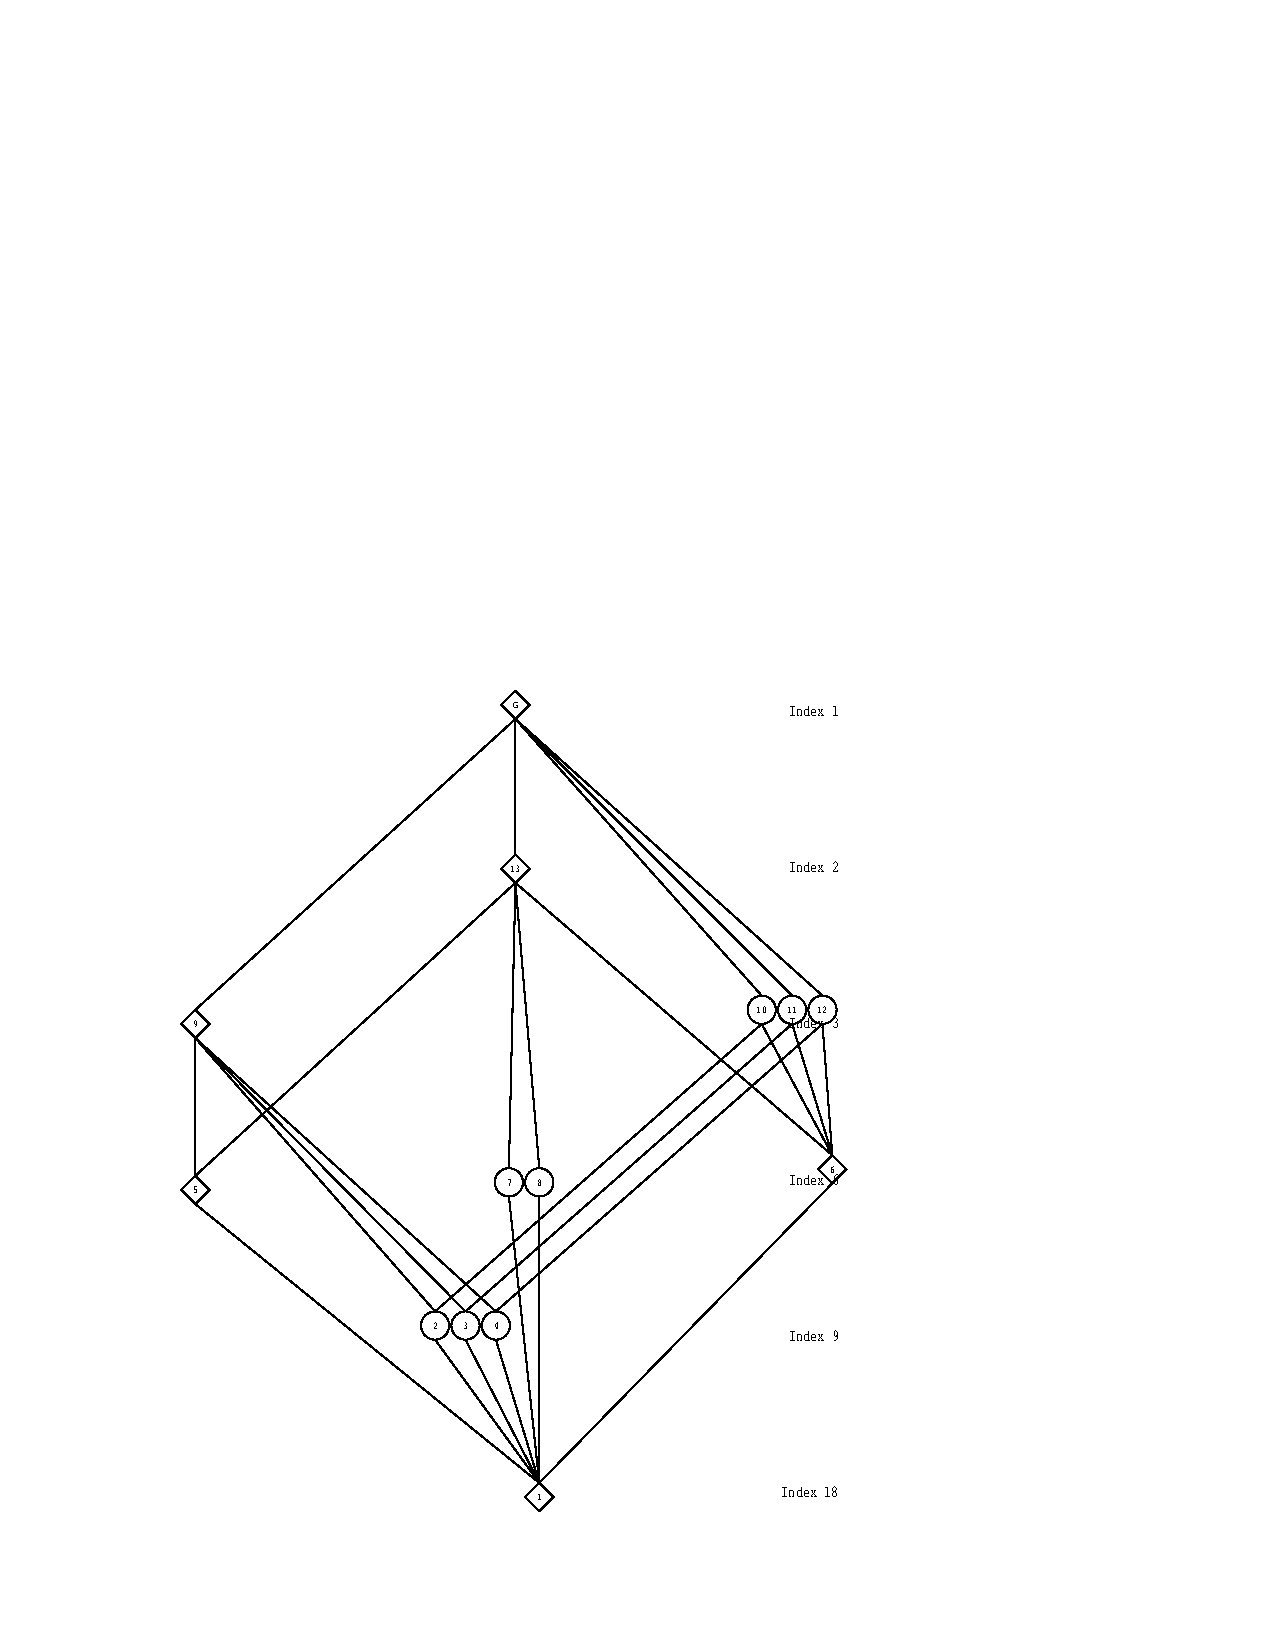
\includegraphics[height=20cm]{s3a3new.pdf}%
\caption{Hasse diagram of $\Sub[S_3 \times A_3]$ drawn by the \xgap\ program.}
\label{fig:s3a3}
\end{center}\end{figure}
{\codesize
\begin{verbatim}
gap> s3 := SymmetricGroup( 3 );;  a3 := AlternatingGroup( 3 );;

\end{verbatim}}
\noindent Of course, $S_3$ has 6 elements, 
$\{ e, (2,3), (1,2), (1,2,3), (1,3,2), (1,3) \}$, 
and is generated by $(1,2)$ and $(1,2,3)$; i.e., $S_3 = \langle (1,2),
(1,2,3)\rangle$.
Its normal subgroup $A_3$ has three elements $\{ e, (1,2,3), (1,3,2)\}$, and
$A_3 = \<(1,2,3)\>$.   Thus, we could have defined {\tt s3} and 
{\tt a3} in \gap\ as follows:
{\codesize
\begin{verbatim}
gap> s3 := Group( (1,2), (1,2,3) );;  a3 := Group( (1,2,3) );;

\end{verbatim}}
\noindent Now define the direct product group {\tt s3a3 := $S_3 \times A_3$}, which has 
$|S_3|\cdot |A_3| = 18$ elements.
{\codesize
\begin{verbatim}
gap> s3a3 := DirectProduct( s3, a3 );  # returns Group([ (1,2), (1,2,3), (4,5,6) ])
gap> Order( s3a3 );                    # returns 18
\end{verbatim}
\noindent (If we had defined {\tt a3s3 := DirectProduct( a3, s3 );}, the result
would have been \\
{\tt Group([ (1,2,3), (4,5), (4,5,6) ])}, which is, of course, isomorphic to
{\tt s3a3}.)}
\\[5pt]
\noindent If you are using the \xgap\ package, an extension of \gap, you can see the
Hasse diagram of the subgroup lattice of a group with the command 
{\tt GraphicSubgroupLattice}.
For example, the following command draws the subgroup lattice of $S_3 \times A_3$
(Figure~\ref{fig:s3a3}):\footnote{When you execute the 
{\tt GraphicSubgroupLattice} command, the initial result is a
diagram showing only the trivial subgroups (e.g., $(e)$ and $S_3\times A_3$).  
To see the full subgroup lattice, you must select {\tt All Subgroups} from the 
{\tt Subgroups} menu.} 
{\codesize
\begin{verbatim}
gap> GraphicSubgroupLattice( s3a3 );

\end{verbatim}}
\noindent \xgap\ depicts normal subgroups with diamonds and non-normal subgroups with circles.  
Conjugacy classes of subgroups are grouped together.
(Thus, a normal subgroup appears by itself.)

In the lattice in Figure~\ref{fig:s3a3}, the
subgroup of index two is the normal subgroup $A_3 \times A_3$. 
Now, $A_3$ has no proper nontrivial subgroups (and thus $\Sub[A_3]$ is just the
two element chain).  Nonetheless, it is clear from the diagram that the subgroup
lattice $\Sub[A_3 \times A_3]$ is isomorphic to $M_4$ (cf.~$\Sub[\Z_2 \times \Z_2]
\cong M_3$).
\\[6pt]
{\bf Remark:} $\Sub[A_3 \times A_3] \cong M_4 \cong \Sub[S_3]$.  Indeed,
\begin{itemize}
\item It is well-known that $\Sub[G]\cong M_4$ iff $G$ is (isomorphic to) $C_3\times C_3$ or $D_3$.
\item  $S_3$ is isomorphic to the dihedral group $D_3$ of order 6, the symmetries of
  an equilateral triangle (three reflections and three rotations; some authors refer
  to $D_3$ as $D_6$.)  We can easily check by hand that $S_3 \cong D_3$, but \gap\
  quickly confirms this fact as follows:
{\codesize
\begin{verbatim}
gap> s3 := SymmetricGroup(3);    # returns Sym( [ 1 .. 3 ] )
gap> d3 := DihedralGroup(6);     # returns <pc group of size 6 with 2 generators>
gap> IsDihedralGroup(s3);        # returns true
\end{verbatim}}
\item $A_3$ is isomorphic to $C_3$.  This is obvious, but let's check it anyway using GAP:
{\codesize
\begin{verbatim}
gap> a3 := AlternatingGroup(3);  # returns Alt( [ 1 .. 3 ] )
gap> Elements(a3);               # returns [ (), (1,2,3), (1,3,2) ]
gap> IsCyclic(a3);               # returns true

\end{verbatim}}
\end{itemize}

\item For our next example, we let {\tt a3 := $A_3$} and {\tt a4 := $A_4$}, the
alternating groups on three and four letters (resp.), and let 
{\tt c2 := $\Z_2$}, the cyclic group or order 2. 
{\codesize
\begin{verbatim}
gap> a3 := AlternatingGroup( 3 );;  a4 := AlternatingGroup( 4 );;
gap> c2 := CyclicGroup(2);
<pc group of size 2 with 1 generators>

gap> a4c2 := DirectProduct( a4, c2 );
<group of size 24 with 3 generators>

gap> a4a3 := DirectProduct( a4, a3 );
Group([ (1,2,3), (2,3,4), (5,6,7) ])

\end{verbatim}}
\begin{figure}[h!]\begin{center}
\vspace{-8cm}
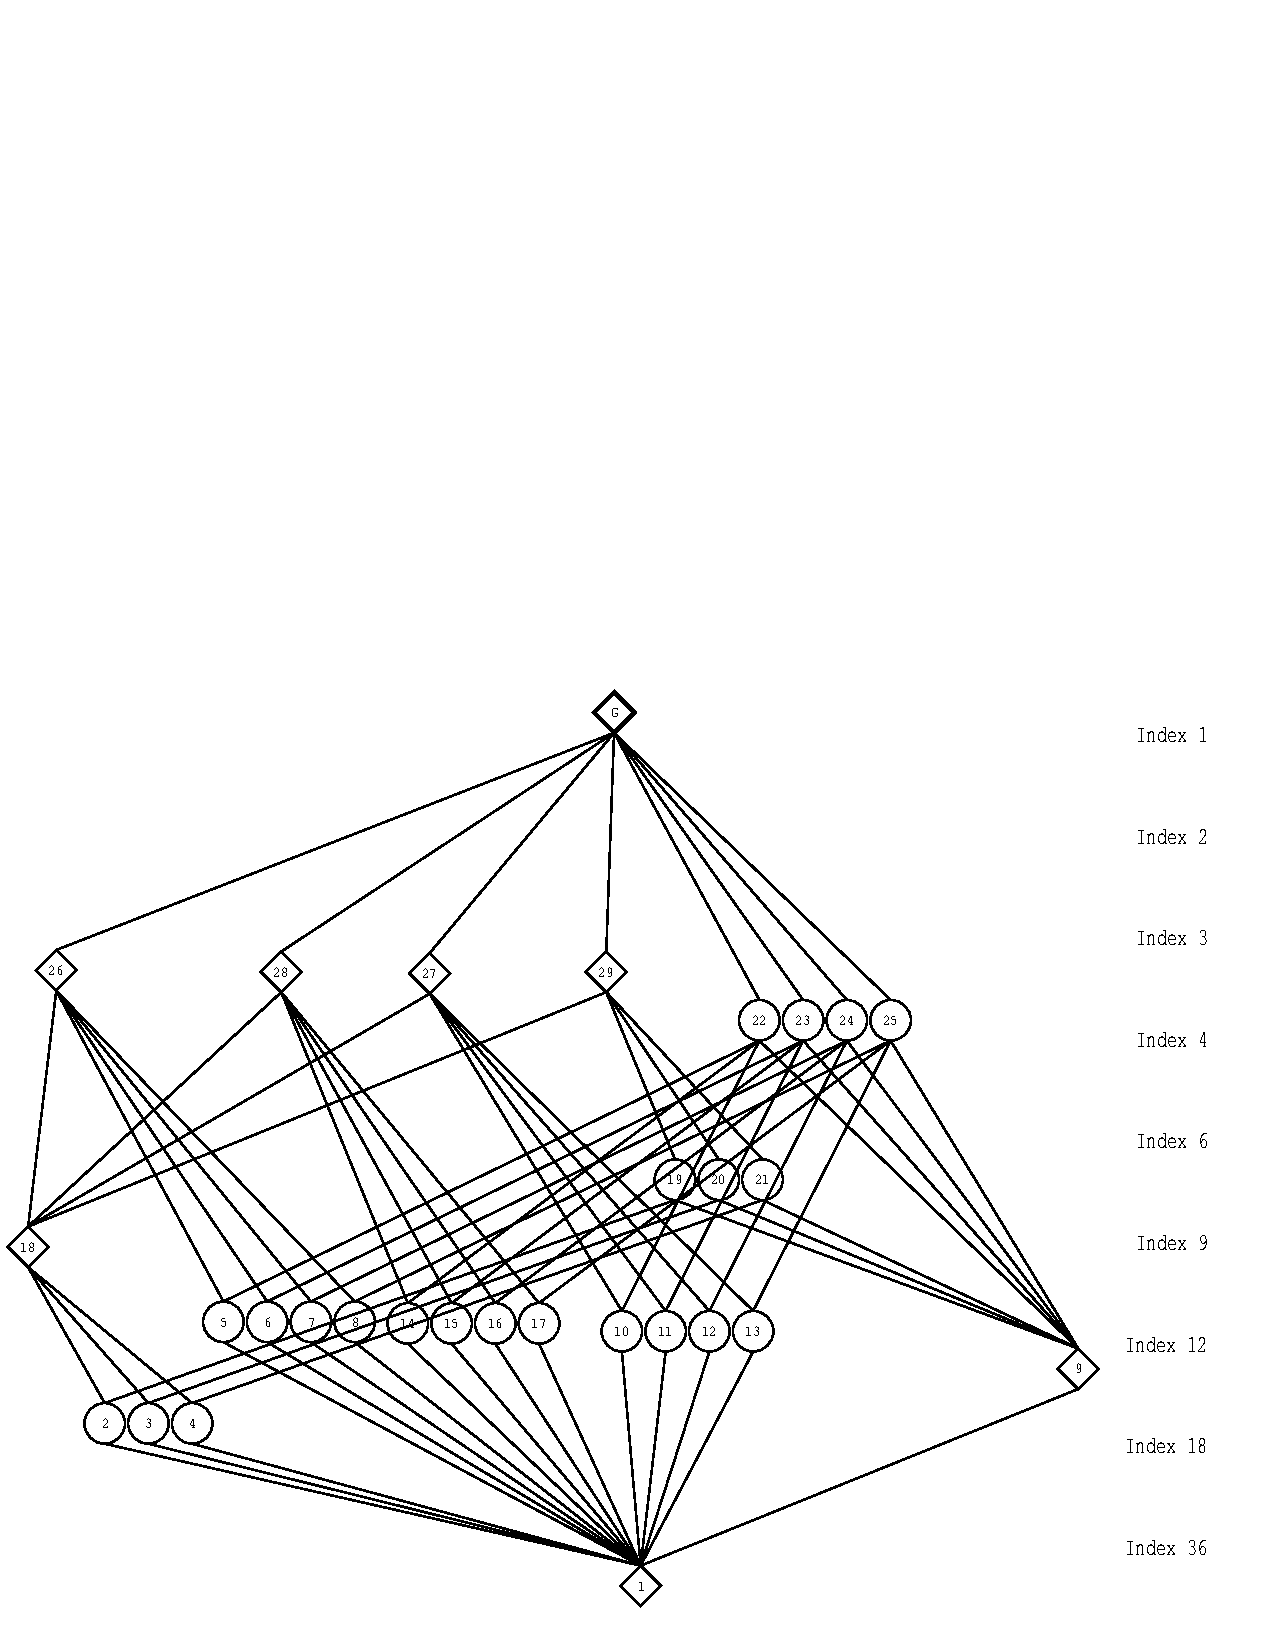
\includegraphics[height=20cm]{a4a3new.pdf}%
\caption{Hasse diagram of $\Sub[A_4 \times A_3]$ drawn by the \xgap\ program.}
\label{fig:a4a3}
\end{center}\end{figure}
\begin{figure}[h!]\begin{center}
\vspace{-8cm}
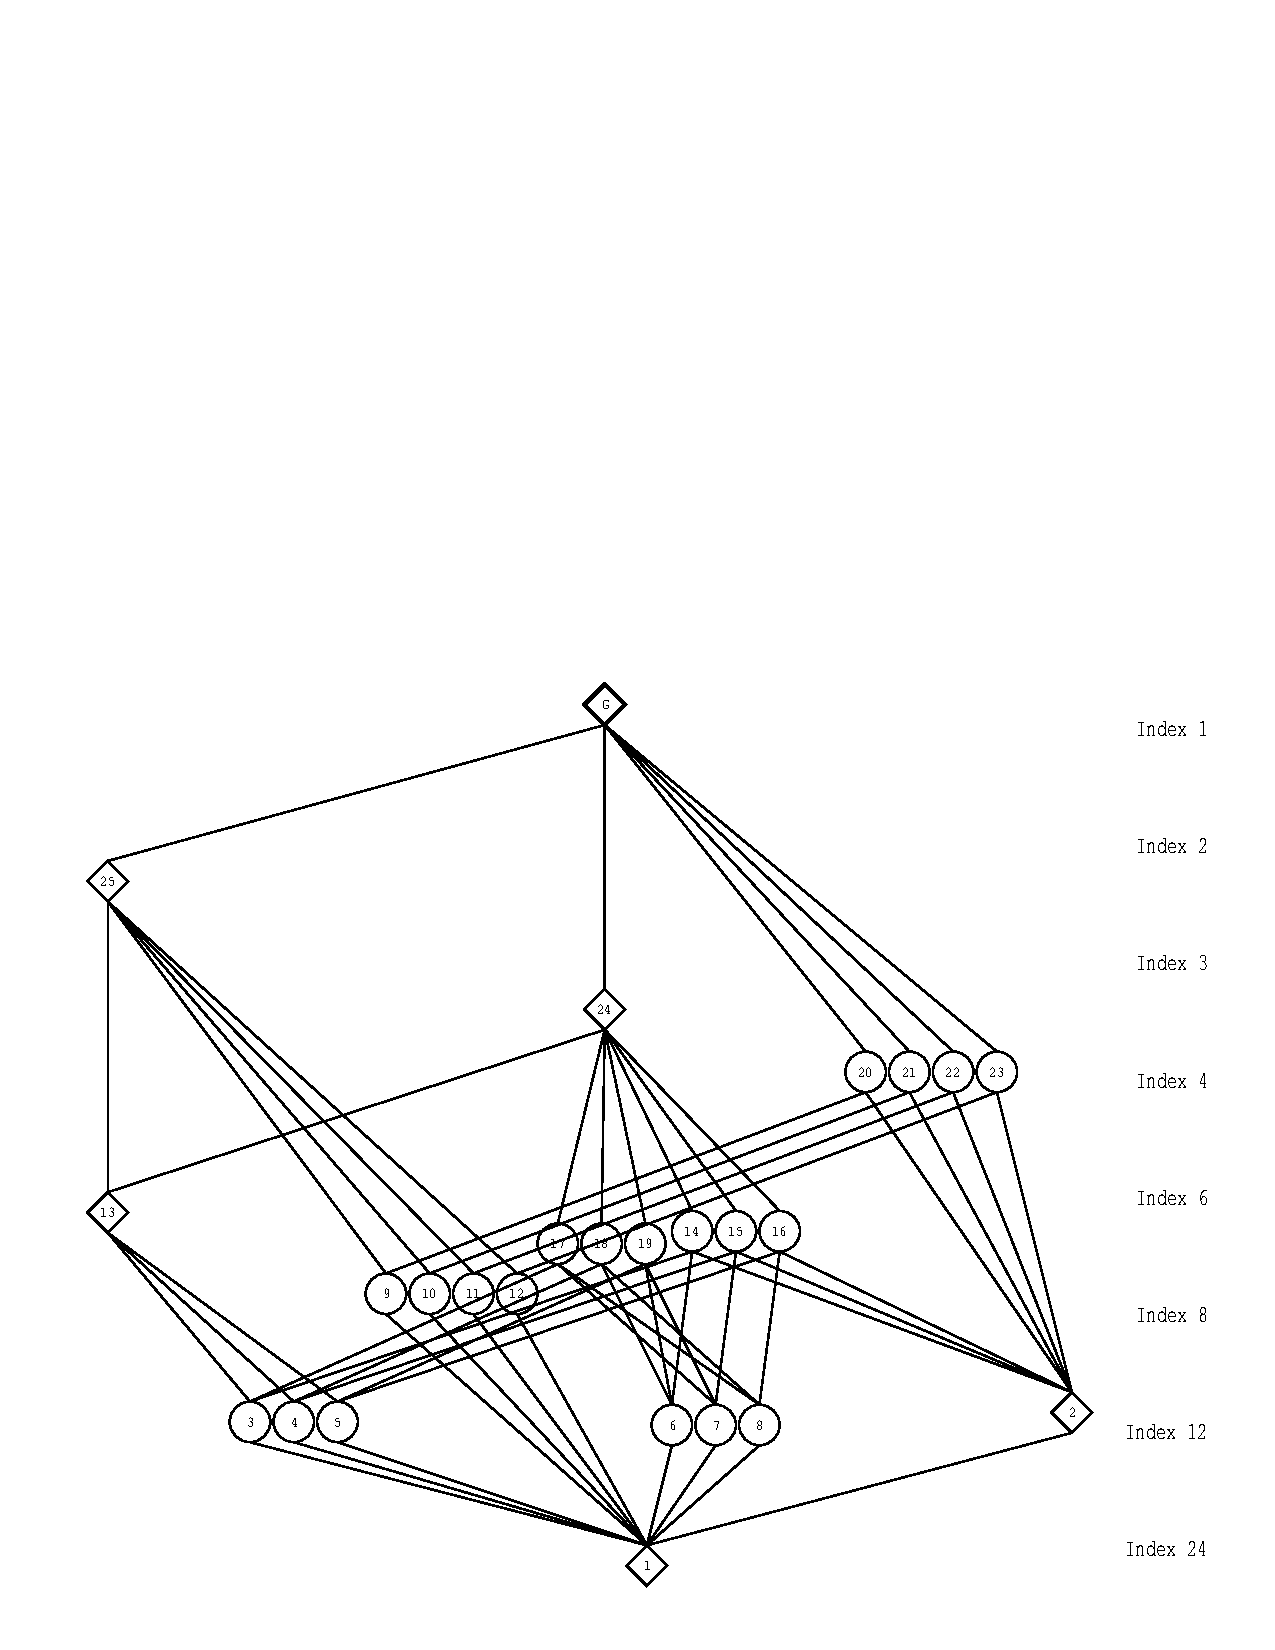
\includegraphics[height=20cm]{a4c2new.pdf}%
\caption{Hasse diagram of $\Sub[A_4 \times \Z_2]$ drawn by the \xgap\ program.}
\label{fig:a4c2}
\end{center}\end{figure}
\begin{figure}[h!]\begin{center}
\vspace{-8cm}
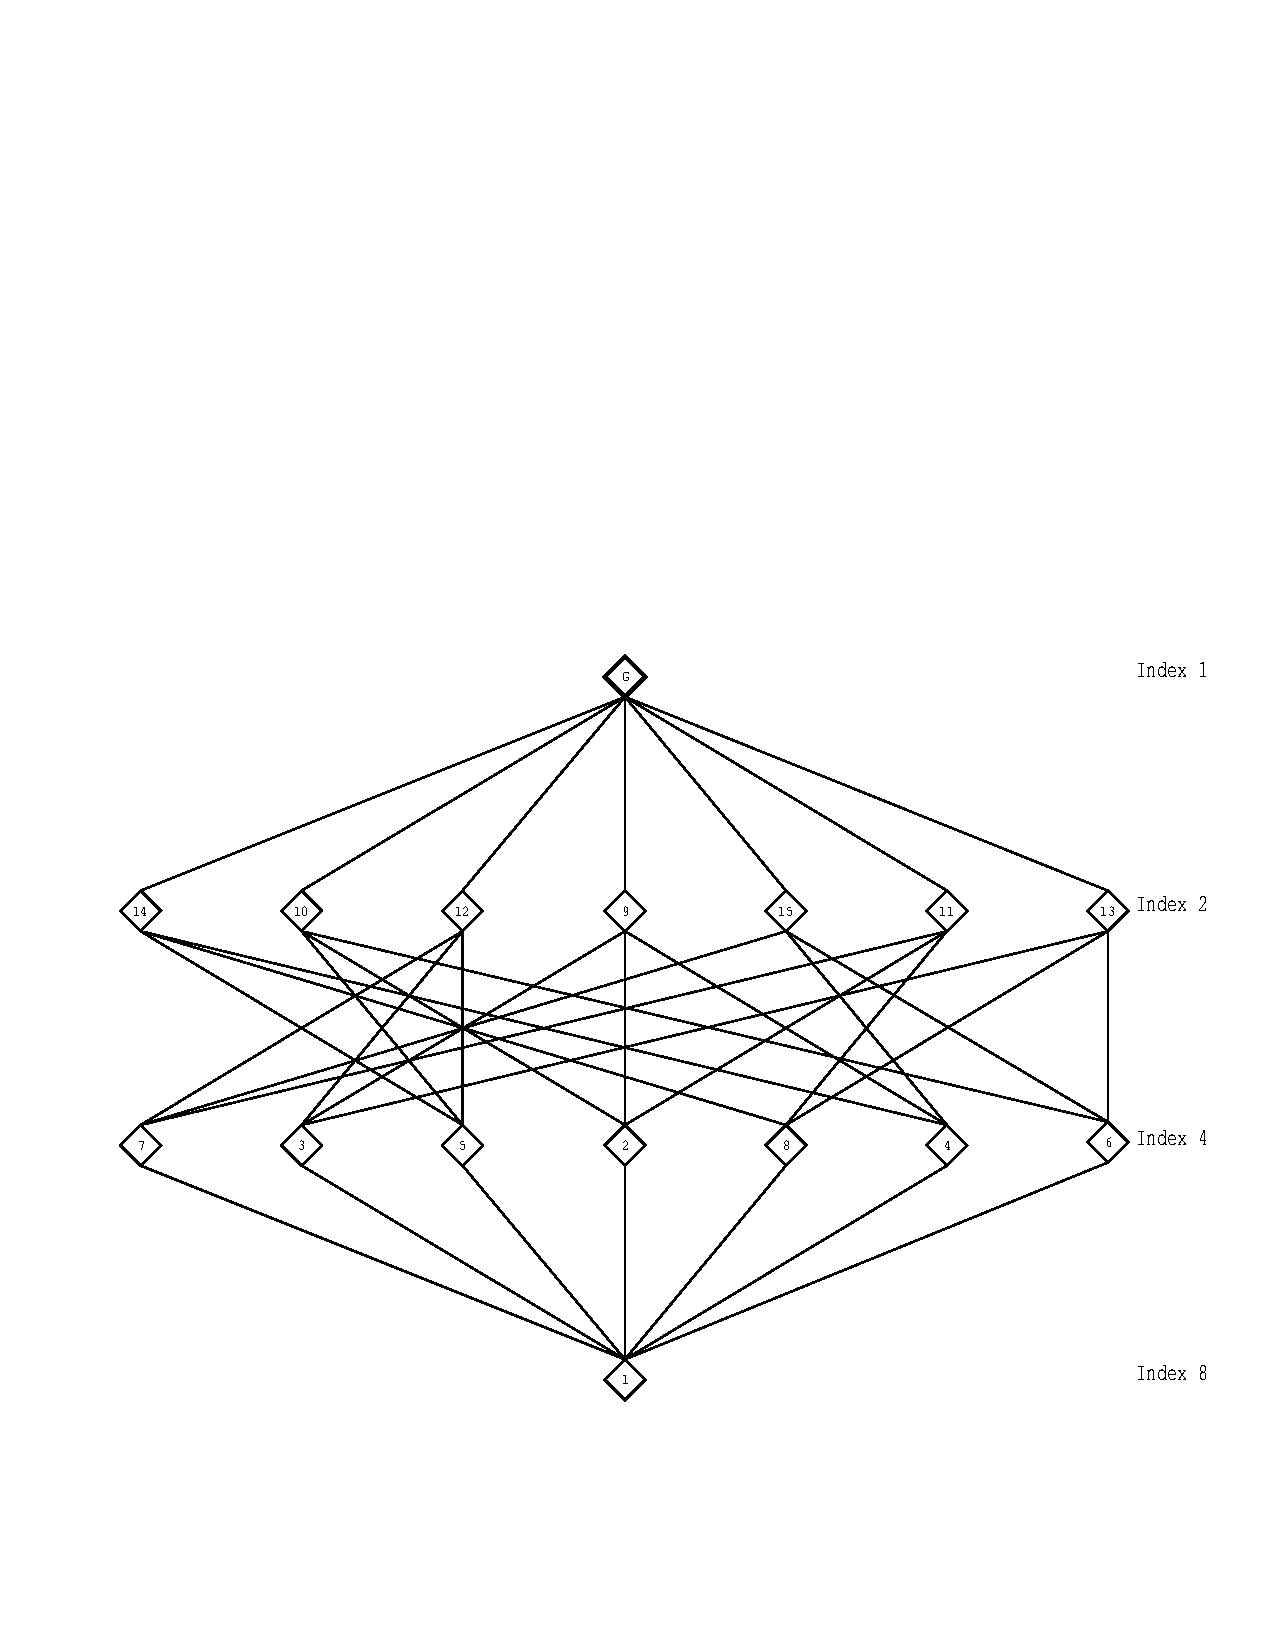
\includegraphics[height=18cm]{v4c2new.pdf}%
\caption{Hasse diagram of $\Sub[V_4 \times \Z_2]$ drawn by the \xgap\ program.}
\label{fig:v4c2}
\end{center}\end{figure}
\noindent If you are using \xgap, the subgroup lattices 
$\Sub[A_4 \times A_3]$ and $\Sub[A_4 \times \Z_2]$ are displayed with
{\tt GraphicSubgroupLattice}.  
{\codesize
\begin{verbatim}
gap> GraphicSubgroupLattice( a4a3 );
gap> GraphicSubgroupLattice( a4c2 );

\end{verbatim}}

\noindent In the subgroup lattice $\Sub[A_4 \times \Z_2]$ (Figure~\ref{fig:a4c2}), 
consider the (maximal) normal subgroup of index 3; 
i.e., the diamond labelled 24.  
The diagram makes clear that this is the subgroup 
$V_4 \times \Z_2$, where $V_4$ is the Klein 4 group.  
It's hard to see exactly what's happening below this subgroup in the full 
$\Sub[A_4 \times \Z_2]$ lattice,
but we can get a handle on $V_4 \times \Z_2$, and draw its subgroup lattice, 
$\Sub[V_4 \times \Z_2]$ (Figure~\ref{fig:v4c2}), with the following commands:
{\codesize
\begin{verbatim}
gap> cclsa4 := ConjugacyClassesSubgroups(a4);
[ Group( () )^G, Group( [ (1,2)(3,4) ] )^G, Group( [ (2,4,3) ] )^G, 
  Group( [ (1,3)(2,4), (1,2)(3,4) ] )^G, 
  Group( [ (1,3)(2,4), (1,2)(3,4), (2,4,3) ] )^G ]
gap> v4 := Representative(cclsa4[4]);
Group([ (1,3)(2,4), (1,2)(3,4) ])
gap> Order(v4);     # returns 4 
gap> IsCyclic(v4);  # returns false (v4 is, indeed, the Klein 4 group)
gap> v4c2 := DirectProduct(v4,c2);
<group of size 8 with 3 generators>
gap> GraphicSubgroupLattice(v4c2);
\end{verbatim}}
\end{enumerate}



\newpage


\newpage 

\subsection{Embeddings and Projections}
\label{sec:embedd-proj-group}
The relation between a group product and its factors is provided via homomorphisms, the embeddings in
the product and the projections from the product. Depending on the kind of product only some of these are
defined.
\begin{itemize}
\item {\tt Embedding( P, nr )}\\[2pt]
returns the {\tt nr}-th embedding in the group product {\tt P}. 
The actual meaning of this embedding is described in the section for the appropriate product.
\item {\tt Projection( P[, nr] )}\\[2pt]
returns the ({\tt nr}-th) projection of the group product {\tt P}. 
The actual meaning of the projection returned is described in the section for the appropriate product.
\end{itemize}
\subsectionspace

\noindent {\it Examples: embeddings and projections of $S_3 \times A_3$.}
\\[6pt]
As above, let 
{\tt s3 := $S_3$} and {\tt a3 := $A_3$}, 
the symmetric and alternating group on three letters (resp.), and let 
{\tt s3a3 := $S_3\times A_3$}.
{\codesize
\begin{verbatim}
gap> s3 := Group( (1,2), (1,2,3) );;  a3 := Group( (1,2,3) );;
gap> s3a3 := DirectProduct( s3, a3 );  # returns Group([ (1,2), (1,2,3), (4,5,6) ])
gap> Order( s3a3 );                    # returns  18

\end{verbatim}}
\noindent The following \gap\ code illustrates the behavior of the commands 
{\tt Embedding} and {\tt Projection}, and the corresponding {\tt Source}, 
{\tt Range}, and {\tt Image} commands (sec.~\ref{sec:mappings}): 
{\codesize
\begin{verbatim}
gap> i1 := Embedding( s3a3, 1 );
1st embedding into Group([ (1,2), (1,2,3), (4,5,6) ])
gap> i2 := Embedding( s3a3, 2 );
2nd embedding into Group([ (1,2), (1,2,3), (4,5,6) ])

gap> Source( i1 );                    # returns Group([ (1,2), (1,2,3) ])
gap> Range( i1 );                     # returns Group([ (1,2), (1,2,3), (4,5,6) ])
gap> Image( i1 );                     # returns Group([ (1,2), (1,2,3) ])
gap> ImagesSource( i1 );              # returns Group([ (1,2), (1,2,3) ])

gap> Source( i2 );                    # returns Group([ (1,2,3) ])
gap> Range( i2 );                     # returns Group([ (1,2), (1,2,3), (4,5,6) ])
gap> Image( i2 );                     # returns Group([ (4,5,6) ])
gap> ImagesSource( i2 );              # returns Group([ (4,5,6) ])

gap> p1 := Projection( s3a3, 1 );
1st projection of Group([ (1,2), (1,2,3), (4,5,6) ])
gap> p2 := Projection( s3a3, 2 );
2nd projection of Group([ (1,2), (1,2,3), (4,5,6) ])

gap> Source( p1 );                    # returns Group([ (1,2), (1,2,3), (4,5,6) ])
gap> Range( p1 );                     # returns Group([ (1,2), (1,2,3) ])
gap> Image( p1 );                     # returns Group([ (1,2), (1,2,3) ])
gap> Image( p1, (1,2,3) );            # returns (1,2,3)
gap> Image( p1, (4,5,6) );            # returns ()
gap> Image( p1, (1,2)(4,5,6) );       # returns (1,2)

gap> Source( p2 );                    # returns Group([ (1,2), (1,2,3), (4,5,6) ])
gap> Range( p2 );                     # returns Group([ (1,2,3) ])
gap> Image( p2 );                     # returns Group([ (1,2,3) ])
gap> Image( p2, (1,2,3) );            # returns ()
gap> Image( p2, (4,5,6) );            # returns (1,2,3)
gap> Image( p2, (1,2)(4,5,6) );       # returns (1,2,3)

gap> Image( p2, (1,2,3)(4,5) );       # Error: (1,2,3)(4,5) is not in Source of p2
brk> quit;                           

gap> Elements( Source( p2 ) );
[ (), (4,5,6), (4,6,5), (2,3), (2,3)(4,5,6), (2,3)(4,6,5), (1,2), 
  (1,2)(4,5,6), (1,2)(4,6,5), (1,2,3), (1,2,3)(4,5,6), (1,2,3)(4,6,5), 
  (1,3,2), (1,3,2)(4,5,6), (1,3,2)(4,6,5), (1,3), (1,3)(4,5,6), (1,3)(4,6,5) ]

gap> Image( p2, (1,2,3)(4,6,5) );     # returns (1,3,2)

\end{verbatim}}
\noindent We could have used the command {\tt UnderlyingRelation}
(sec.~\ref{sec:properties-of-mappings}) to display most of this information
at once: 
{\codesize
\begin{verbatim}
gap> Elements(UnderlyingRelation( i1 ));
[ Tuple( [ (), () ] ), Tuple( [ (2,3), (2,3) ] ), Tuple( [ (1,2), (1,2) ] ), 
  Tuple( [ (1,2,3), (1,2,3) ] ), Tuple( [ (1,3,2), (1,3,2) ] ), 
  Tuple( [ (1,3), (1,3) ] ) ]

gap> Elements(UnderlyingRelation( i2 ));
[ Tuple( [ (), () ] ), Tuple( [ (1,2,3), (4,5,6) ] ), 
  Tuple( [ (1,3,2), (4,6,5) ] ) ]

gap> Elements(UnderlyingRelation( p1 ));
[ Tuple( [ (), () ] ), Tuple( [ (4,5,6), () ] ), Tuple( [ (4,6,5), () ] ), 
  Tuple( [ (2,3), (2,3) ] ), Tuple( [ (2,3)(4,5,6), (2,3) ] ), 
  Tuple( [ (2,3)(4,6,5), (2,3) ] ), Tuple( [ (1,2), (1,2) ] ), 
  Tuple( [ (1,2)(4,5,6), (1,2) ] ), Tuple( [ (1,2)(4,6,5), (1,2) ] ), 
  Tuple( [ (1,2,3), (1,2,3) ] ), Tuple( [ (1,2,3)(4,5,6), (1,2,3) ] ), 
  Tuple( [ (1,2,3)(4,6,5), (1,2,3) ] ), Tuple( [ (1,3,2), (1,3,2) ] ), 
  Tuple( [ (1,3,2)(4,5,6), (1,3,2) ] ), Tuple( [ (1,3,2)(4,6,5), (1,3,2) ] ), 
  Tuple( [ (1,3), (1,3) ] ), Tuple( [ (1,3)(4,5,6), (1,3) ] ), 
  Tuple( [ (1,3)(4,6,5), (1,3) ] ) ]

gap> Elements(UnderlyingRelation( p2 ));
[ Tuple( [ (), () ] ), Tuple( [ (4,5,6), (1,2,3) ] ), 
  Tuple( [ (4,6,5), (1,3,2) ] ), Tuple( [ (2,3), () ] ), 
  Tuple( [ (2,3)(4,5,6), (1,2,3) ] ), Tuple( [ (2,3)(4,6,5), (1,3,2) ] ), 
  Tuple( [ (1,2), () ] ), Tuple( [ (1,2)(4,5,6), (1,2,3) ] ), 
  Tuple( [ (1,2)(4,6,5), (1,3,2) ] ), Tuple( [ (1,2,3), () ] ), 
  Tuple( [ (1,2,3)(4,5,6), (1,2,3) ] ), Tuple( [ (1,2,3)(4,6,5), (1,3,2) ] ), 
  Tuple( [ (1,3,2), () ] ), Tuple( [ (1,3,2)(4,5,6), (1,2,3) ] ), 
  Tuple( [ (1,3,2)(4,6,5), (1,3,2) ] ), Tuple( [ (1,3), () ] ), 
  Tuple( [ (1,3)(4,5,6), (1,2,3) ] ), Tuple( [ (1,3)(4,6,5), (1,3,2) ] ) ]
gap> 
\end{verbatim}}
But note that {\tt UnderlyingRelation} does not tell the whole story.  In particular,
it is impossible to infer from the output of {\tt UnderlyingRelation} the full 
{\tt Source} and {\tt Range} of a general mapping.
\\

\subsection{Semidirect Products}
The semidirect product of a group $N$
with a group $G$ acting on $N$ via a homomorphism $\alpha$ from $G$ into
the automorphism group of $N$ is the Cartesian product $G \times N$ with the
multiplication 
\[
(g, n) \cdot (h, m) = (gh, n\bar{h} \cdot m)= (gh, n^{h\alpha} m).
\]
\begin{itemize}
\item {\tt SemidirectProduct( $G, \, \alpha, \, N$ )}
\item {\tt SemidirectProduct( $autgp, \, N$ )}\\[2pt]
constructs the semidirect product of $N$ with $G$ acting via $\alpha$, where $\alpha$
must be a homomorphism from $G$ into a group of automorphisms of $N$.
\\[5pt]
If $N$ is a full row space over a field $\F$, $\alpha$ must be a homomorphism from
$G$ into a matrix group of the right dimension over a subfield of $\F$, or into a
permutation group (in this case permutation matrices are taken).
\\[5pt]
In the second variant, $autgp$ must be a group of automorphism of $N$, it is a
shorthand for {\tt SemidirectProduct( $autgp$, IdentityMapping($autgp$), $N$ )}. Note
that (unless $autgrp$ has been obtained by the operation  {\tt AutomorphismGroup})
you have to test {\tt IsGroupOfAutomorphisms( $autgrp$ )} to ensure that \gap\ knows that 
$autgrp$ consists of group automorphisms.
{\codesize
\begin{verbatim}
gap> n:=AbelianGroup(IsPcGroup,[5,5]);
<pc group of size 25 with 2 generators>
gap> au:=DerivedSubgroup(AutomorphismGroup(n));;
gap> Size(au);                      # returns  120
gap> p:=SemidirectProduct(au,n);
<permutation group with 5 generators>
gap> Size(p);                       # returns 3000
gap> n:=Group((1,2),(3,4));;
gap> au:=AutomorphismGroup(n);;
gap> au:=First(Elements(au),i->Order(i)=3);;
gap> au:=Group(au);
<group with 1 generators>
gap> SemidirectProduct(au,n);
Error, no method found! For debugging hints type ?Recovery from NoMethodFound
Error, no 2nd choice method found for `IsomorphismPcGroup' on 1 arguments
gap> IsGroupOfAutomorphisms(au);
true
gap> SemidirectProduct(au,n);
<pc group with 3 generators>
gap> n:=AbelianGroup(IsPcGroup,[2,2]);
<pc group of size 4 with 2 generators>
gap> au:=AutomorphismGroup(n);
<group of size 6 with 2 generators>
gap> apc:=IsomorphismPcGroup(au);
CompositionMapping( Pcgs([ (2,3), (1,2,3) ]) ->
[ f1, f2 ], <action isomorphism> )
gap> g:=Image(apc);
Group([ f1, f2 ])
gap> apci:=InverseGeneralMapping(apc);
[ f1*f2^2, f1*f2 ] -> [ Pcgs([ f1, f2 ]) -> [ f1*f2, f2 ],
Pcgs([ f1, f2 ]) -> [ f2, f1 ] ]
gap> IsGroupHomomorphism(apci);
true
gap> p:=SemidirectProduct(g,apci,n);
<pc group of size 24 with 4 generators>
gap> IsomorphismGroups(p,Group((1,2,3,4),(1,2)));
[ f1, f2, f3, f4 ] -> [ (2,3), (2,3,4), (1,4)(2,3), (1,2)(3,4) ]
gap> SemidirectProduct(SU(3,3),GF(9)^3);
<matrix group of size 4408992 with 3 generators>
gap> SemidirectProduct(Group((1,2,3),(2,3,4)),GF(5)^4);
<matrix group of size 7500 with 3 generators>
gap> g:=Group((3,4,5),(1,2,3));;
gap> mats:=[[[Z(2^2),0*Z(2)],[0*Z(2),Z(2^2)^2]],
> [[Z(2)^0,Z(2)^0], [Z(2)^0,0*Z(2)]]];;
gap> hom:=GroupHomomorphismByImages(g,Group(mats),[g.1,g.2],mats);;
gap> SemidirectProduct(g,hom,GF(4)^2);
<matrix group of size 960 with 3 generators>
gap> SemidirectProduct(g,hom,GF(16)^2);
<matrix group of size 15360 with 4 generators>
\end{verbatim}}
\noindent For the semidirect product $P$ of $G$ with $N$, {\tt Embedding( $P$, 1 )}
embeds $G$, {\tt Embedding( $P$, 2 )} embeds $N$. The operation {\tt Projection(P)}
returns the projection of $P$ onto $G$.\footnote{{\it Op.~cit.}, sec.~47.6.}
{\codesize
\begin{verbatim}
gap> Size(Image(Embedding(p,1)));    # returns 6
gap> Embedding(p,2);
[ f1, f2 ] -> [ f3, f4 ]
gap> Projection(p);
[ f1, f2, f3, f4 ] -> [ f1, f2, <identity> of ..., <identity> of ... ]

\end{verbatim}}

\end{itemize}
\subsectionspace

\subsection{Subdirect Products\protect\footnotemark}
\footnotetext{{\it Ibid.}, sec.~47.3.} 
The subdirect product of the groups $G$ and $H$ with respect to the epimorphisms
$\varphi: G \rightarrow A$ and
$\psi: H \rightarrow A$
(for a common group $A$) is the subgroup of the direct product $G \times H$
consisting of the elements $(g, h)$ for which $\varphi(g) = \psi(h)$ . 
It is the pull-back of the diagram:
\begin{figure}[h]
\begin{tikzpicture}[description/.style={fill=white,inner sep=2pt}]
\matrix (m) [matrix of math nodes, row sep=3em,
column sep=2.5em, text height=1.5ex, text depth=0.25ex]
{  & & G \\
 H & & A\\ };
\path[->>,font=\footnotesize]
(m-1-3) edge node[right] {$\varphi$} (m-2-3)
(m-2-1) edge node[above] {$\psi$} (m-2-3);
%\path[->,loosely dashed,font=\scriptsize]
%(m-2-1) edge node[below] {$ \psi $} (m-1-3);
\end{tikzpicture}
\end{figure}
\begin{itemize}
\item {\tt SubdirectProduct( $G$ , $H$, $\varphi$, $\psi$ )}\\
constructs the subdirect product of $G$ and $H$ with respect to the epimorphisms $\varphi$ from $G$ onto a group
$A$ and $\psi$ from $H$ onto the same group $A$.
For a subdirect product {\tt P}, the operation {\tt Projection(P, nr)} returns
the projection on the {\tt nr}-th factor. (In general the factors do not embed
in a subdirect product.)
{\codesize
\begin{verbatim}
gap> g:=Group((1,2,3),(1,2));;
gap> hom:=GroupHomomorphismByImagesNC(g,g,[(1,2,3),(1,2)],[(),(1,2)]);
[ (1,2,3), (1,2) ] -> [ (), (1,2) ]
gap> s:=SubdirectProduct(g,g,hom,hom);
Group([ (1,2,3), (1,2)(4,5), (4,5,6) ])
gap> Size(s);                                # returns 18
gap> p:=Projection(s,2);
2nd projection of Group([ (1,2,3), (1,2)(4,5), (4,5,6) ])
gap> Image(p,(1,3,2)(4,5,6));                # returns (1,2,3)

\end{verbatim}}
\item {\tt SubdirectProducts( $G$, $H$ )}\\
computes all subdirect products of $G$ and $H$ up to conjugacy in Parent($G$) $\times$ Parent($H$). The
subdirect products are returned as subgroups of this direct product.
\end{itemize}
\subsectionspace

\subsection{Wreath Products\protect\footnotemark}
\footnotetext{{\it Ibid.}, sec.~47.4.} 
The \emph{wreath product} of a group $G$ with a permutation group $P$ acting on $n$
points is the semidirect product of the normal subgroup $G^n$ with the group $P$
which acts on $G^n$ by permuting the components. 
\begin{itemize}
\item {\tt WreathProduct( $G$, $P$ )}
\item {\tt WreathProduct( $G$, $H$ [, $hom$] )}\\
constructs the wreath product of the group $G$ with the permutation group $P$ 
(acting on its {\tt MovedPoints}). 
\\[4pt]
The second usage constructs the wreath product of the group $G$ with the image of the
group $H$ under $hom$ where $hom$ must be a homomorphism from $H$ into a permutation
group.  If $hom$ is not given, and $P$ is not a permutation group, then $hom$ is
taken to be the result of {\tt IsomorphismPermGroup(P)} (whose degree may be
dependent on the method and thus is not well-defined!).
\\[4pt]
If $W$ is a wreath product of $G$ with a permutation group $P$ of degree $n$, and 
$1 \leq nr \leq n$, then the operation
{\tt Embedding( $W$, $nr$ )} provides the embedding of $G$ in the $nr$-th component
of the direct product of the base group $G^n$ of $W$. {\tt Embedding( $W$, $n+1$ )}
is the embedding of $P$ in $W$. The operation {\tt Projection( $W$ )} 
gives the projection onto the acting group $P$.
{\codesize
\begin{verbatim}
gap> g:=Group((1,2,3),(1,2));     # the symmetric group on {1, 2, 3}
gap> p:=Group((1,2,3));           # the alternating group on {1, 2, 3}
gap> w:=WreathProduct(g,p);
Group([ (1,2,3), (1,2), (4,5,6), (4,5), (7,8,9), (7,8), (1,4,7)(2,5,8)(3,6,9) ])
gap> Order(w);                    # returns 648
\end{verbatim}}
The wreath product {\tt w} is the semidirect product $S_3 \times S_3 \times S_3
\rtimes A_3$, which of course has order $|S_3|^3\cdot |A_3| = 6^3 \cdot 6 = 648$.

{\codesize
\begin{verbatim}
gap> Embedding(w,1);
1st embedding into Group( [ (1,2,3), (1,2), (4,5,6), (4,5), (7,8,9), (7,8),
(1,4,7)(2,5,8)(3,6,9) ] )
gap> Image(Embedding(w,3));     # returns Group([ (7,8,9), (7,8) ])
gap> Image(Embedding(w,4));     # returns Group([ (1,4,7)(2,5,8)(3,6,9) ])
gap> Image(Projection(w),(1,4,8,2,6,7,3,5,9));  # returns (1,2,3)

\end{verbatim}}
\item {\tt WreathProductImprimitiveAction( $G$, $H$ )}\\
for two permutation groups $G$ and $H$ this function constructs the wreath product of $G$ and $H$ in the
imprimitive action. If $G$ acts on $l$ points and $H$ on $m$ points this action will
be on $l^m$ points, it will be imprimitive with $m$ blocks of size $l$ each.
The operations {\tt Embedding} and {\tt Projection} operate on this product as described for general wreath products.
{\codesize
\begin{verbatim}
gap> w:=WreathProductImprimitiveAction(g,p);;
gap> LargestMovedPoint(w);      # returns 9

\end{verbatim}}
\item {\tt WreathProductProductAction( $G$, $H$ )}\\
for two permutation groups $G$ and $H$ this function constructs the wreath product in
product action. If $G$ acts on $l$ points and $H$ on m points this action will be on
$l^m$ points.
\\[4pt]
The operations {\tt Embedding} and {\tt Projection} operate on this product as described for general wreath products.
{\codesize
\begin{verbatim}
gap> w:=WreathProductProductAction(g,p);
<permutation group of size 648 with 7 generators>
gap> LargestMovedPoint(w);      # returns 27
\end{verbatim}}
\end{itemize}

\newpage

\section{Matrix Groups and the Classical Groups}
\subsection{Fields}
This subsection contains a highly abridged version of chapters 56 and 57 of the \gap\
manual.  Initially, my main goal was to collect the few things we'll need to compute
with matrix groups in \gap, but because the subject of fields is so important and
interesting, I've included a bit more information here than is required for working
with matrix groups.
\\[4pt]
A \emph{division ring} is a ring in which every non-zero element has an inverse. The most
important class of division rings are the commutative ones, which are called \emph{fields}.
\\[4pt]
If a field $F$ is a subfield of a commutative ring $C$, $C$ can be considered as a
vector space over the (left) acting domain $F$. In this situation, we call $F$ the
\emph{field of definition} of $C$. Each field in \gap\ is represented as a vector
space over a subfield, thus each field is in fact a field extension in a natural way,
which is used by functions such as {\tt Norm} and {\tt Trace}.
\begin{itemize}
\item {\tt IsDivisionRing( $D$ )}\\
A \emph{division ring} is a nontrivial associative algebra $D$ in which each nonzero
element has a multiplicative inverse. 
In \gap\ every division ring is a vector space over a division ring (possibly over
itself). Note that being a division ring is not a property that a ring can acquire,
because a ring is usually not represented as a vector space. 
The field of coefficients is stored as {\tt LeftActingDomain( $D$ )}.

\item {\tt IsField( D )}\\
A \emph{field} is a commutative division ring.
{\codesize
\begin{verbatim}
gap> IsField( GaloisField(16) );          # returns true (the field with 16 elements)
gap> IsField( Rationals );                # returns true (the field of rationals)
gap> q:= QuaternionAlgebra( Rationals );; # (a noncommutative division ring)
gap> IsField( q );  IsDivisionRing( q );  # returns false true
gap> mat:= [ [ 1 ] ];; a:= Algebra( Rationals, [ mat ] );;
gap> IsDivisionRing( a );                 # returns false  (since the algebra a
                                          # was not constructed as a division ring)
\end{verbatim}}
\item {\tt Field( $z,\dots$ )}
\item {\tt Field( list )}
\item {\tt Field( $F$, list )}\\
returns the smallest field $K$ that contains all the elements $z,\dots$, or (resp.) the
smallest field $K$ that contains all elements in {\tt list}. 
If no subfield $F$ is given, $K$ is constructed as a field over itself. In the third form, {\tt Field} constructs the field generated
by the field $F$ and the elements in the list {\tt list}, as a vector space over $F$.
\item {\tt DefaultField( $z,\dots$ )}
\item {\tt DefaultField( list )}\\
returns a field $K$ that contains all the elements $z, \dots$, or (resp.) a field $K$ that contains all elements
in the list {\tt list}.  The result need not be the smallest field in which the elements lie, 
in contrast to the field returned by the {\tt Field} command. For example, for
elements from cyclotomic fields, {\tt DefaultField} returns the smallest cyclotomic
field in which the elements lie, but the elements may lie in a smaller number field
which is not a cyclotomic field. 
\item \verb.Z(p,d).
\item \verb.Z(p^d).\\
For creating elements of a finite field the function {\tt Z} can be used. The call
{\tt Z(p,d)} (alternatively \verb.Z(p^d).) returns the designated generator of the
multiplicative group of the finite field with $p^d$ elements. Here $p$ must be a prime.
\\[4pt]
\gap\ can represent elements of all finite fields \verb|GF(p^d)| such that
either (1) \verb|p^d <= 65536| (in which case an extremely efficient internal
representation is used); (2) {\tt d = 1}, (in which case, for large {\tt p}, the
field is represented using the machinery of Residue Class Rings (see section
14.4 of the \gap\ manual) or (3) if the Conway Polynomial of
degree {\tt d} over {\tt GF(p)} is known, or can be computed.
If you attempt to construct an element of \verb|GF(p^d)| 
for which \verb|d > 1| and the relevant Conway Polynomial
is not known, and not necessarily easy to find (see 57.5.2), 
then \gap\ will stop with an error and enter the break loop. If you leave this
break loop by entering return; \gap\ will attempt to compute the Conway 
Polynomial, which may take a very long time.
\\[4pt]
The root returned by {\tt Z} is a generator of the multiplicative group of the finite
field with $p d$ elements, which is cyclic. The order of the element is of course
$p^d-1$.  The $p^d-1$ different powers of the root are exactly the nonzero elements
of the finite field. Thus all nonzero elements of the finite field with $p^d$
elements can be entered as \verb.Z(p^d)^i.. Note that this is also the form that
\gap\ uses to output those elements when they are stored in the internal
representation. In larger fields, it is more convenient to enter and print elements
as linear combinations of powers of the  primitive element. 
(See section 57.6 of the \gap\ manual.)
\\[4pt]
The additive neutral element is {\tt 0*Z(p)}. 
%It is different from the integer 0 in
%subtle ways. First {\tt IsInt( 0*Z(p) } is false and {\tt IsFFE( 0*Z(p) )}is true,
%whereas it is just the other way around for the integer 0.
The multiplicative neutral element is \verb.Z(p)^0.. 
It is different from the integer 1, not only in the obvious way -- e.g.,
\verb.Z(2)^0. {\tt +} \verb.Z(2)^0. is {\tt 0*Z(2)},  while {\tt 1+1} is {\tt 2} --
but also in 
more subtle ways.\footnote{See section 57.1 of the \gap\ manual \cite{gapmanual}.}
%First IsInt(
%Z(p)^0 ) (see 14.1.1) is false and IsFFE( Z(p)^0 ) (see 57.1.1) is true, whereas it is just the other way
%around for the integer 1. 
{\codesize
\begin{verbatim}
# some finite fields
gap> Z(2);                        # returns Z(2)^0
gap> Field( Z(2) );               # returns GF(2)
gap> Elements( Field( Z(2) ) );   # returns [ 0*Z(2), Z(2)^0 ]

gap> Z(5);                        # returns Z(5)
gap> Field( Z(5) );               # returns GF(5)
gap> Elements( Field( Z(5) ) );   # returns [ 0*Z(5), Z(5)^0, Z(5), Z(5)^2, Z(5)^3 ]

gap> Z(32);                       # returns Z(2^5)
gap> Field( Z(32) );              # returns GF(2^5)

gap> Z(2)+Z(2); Z(2)*Z(2);        # returns 0*Z(2)  Z(2)^0
gap> Z(5)+Z(5); Z(5)*Z(5);        # returns Z(5)^2  Z(5)^2
gap> Z(32)+Z(32); Z(32)*Z(32);    # returns 0*Z(2)  Z(2^5)^2

gap> Field(Z(4)); Field(Z(8));    # returns GF(2^2)  GF(2^3)
gap> Elements( Field( Z(4) ) );   # returns [ 0*Z(2), Z(2)^0, Z(2^2), Z(2^2)^2 ]
gap> Elements( Field( Z(8) ) );   # returns [ 0*Z(2), Z(2)^0, Z(2^3), Z(2^3)^2, Z(2^3)^3, ...
                                                  ..., Z(2^3)^4, Z(2^3)^5, Z(2^3)^6 ]
gap> Field( [ Z(4), Z(8) ] );     # returns GF(2^6) (the field of 64 elements)

\end{verbatim}}
% # some abelian number fields
% gap> Field( E(9) );               # returns CF(9)
% gap> Field( CF(4), [ E(9) ] );    # returns AsField( GaussianRationals, CF(36) )
% gap> f1:= Field( EB(5) );         # returns NF(5,[ 1, 4 ])
% gap> f2:= DefaultField( EB(5) );  # returns CF(5)
% gap> f1 = f2;                     # returns false
% gap> IsSubset( f2, f1 );          # returns true
\noindent Since finite field elements are scalars, the operations 
{\tt Characteristic, One, Zero, Inverse, AdditiveInverse, Order} 
can be applied to them.\footnote{For a full description of these operations, 
see the Gap manual \cite{gapmanual} sec.~30.10.} 
{\codesize
\begin{verbatim}
gap> Characteristic( Z( 16 )^10 );       # returns 2
gap> Characteristic( Z( 9 )^2 );         # returns 3
gap> Characteristic( [ Z(4), Z(8) ] );   # returns 2
gap> One( Z(9) );                        # returns Z(3)^0
gap> One( 0*Z(4) );                      # returns Z(2)^0
gap> Zero(Z(125));                       # returns 0*Z(5)
gap> Inverse( Z(9) );                    # returns Z(3^2)^7
gap> AdditiveInverse( Z(9) );            # returns Z(3^2)^5
gap> Order( Z(9)^7 );                    # returns 8

\end{verbatim}}
\end{itemize}

%\subsection{Matrix groups\protect\footnotemark}
%\footnotetext{See Chapter 42 of the \gap\ manual~\cite{gapmanual} for more details.}
\subsection{Matrix groups}\hspace{-2mm}\footnote{See Chapter 42 of the \gap\ manual~\cite{gapmanual} for more details.}
Matrix groups are groups generated by invertible square matrices.\\
For example,
{\codesize
\begin{verbatim}
gap> m1 := [ [ Z(3)^0, Z(3)^0, Z(3) ],
>            [ Z(3), 0*Z(3), Z(3) ],
>            [ 0*Z(3), Z(3), 0*Z(3) ] ];;
gap> m2 := [ [ Z(3), Z(3), Z(3)^0 ],
>            [ Z(3), 0*Z(3), Z(3) ],
>            [ Z(3)^0, 0*Z(3), Z(3) ] ];;
gap> m := Group( m1, m2 );
Group(
[ [ [ Z(3)^0, Z(3)^0, Z(3) ], [ Z(3), 0*Z(3), Z(3) ], [ 0*Z(3), Z(3), 0*Z(3) ] ],
[ [ Z(3), Z(3), Z(3)^0 ], [ Z(3), 0*Z(3), Z(3) ], [ Z(3)^0, 0*Z(3), Z(3) ] ] ])
\end{verbatim}}
\noindent Some attributes and operations available for matrix groups are the following:
\begin{itemize}
\item {\tt IsMatrixGroup( grp )}
\\[4pt]
For most operations, \gap\ only provides methods for finite matrix groups. Many calculations in finite matrix
groups are done via a NiceMonomorphism (see 38.5) that represents a faithful action on vectors.
\item {\tt DimensionOfMatrixGroup( matgrp )}\\
returns the dimension of the matrix group {\tt matgrp}.
\item {\tt DefaultFieldOfMatrixGroup( matgrp )}\\ A
returns a field containing all the matrix entries of all elements of {\tt matgrp}. 
It is not guaranteed to be the smallest field with this property.
\item {\tt FieldOfMatrixGroup( matgrp )}\\
returns the smallest field containing all the matrix entries of all elements of {\tt matgrp}. 
As the calculation of this can be hard, this should onlybe used if one really needs
the smallest field, use {\tt DefaultFieldOfMatrixGroup} to get (for example) the characteristic.
\item {\tt TransposedMatrixGroup( matgrp )}\\
returns the transpose of the matrix group {\tt matgrp}. 
The transpose of the transpose of {\tt matgrp} is identical to {\tt matgrp}.
{\codesize
\begin{verbatim}
gap> DimensionOfMatrixGroup(m);       # returns 3
gap> DefaultFieldOfMatrixGroup(m);    # returns GF(3)

gap> G := Group( [[0,-1],[1,0]] );; 
gap> IsMatrixGroup(G);                # returns true
gap> T := TransposedMatrixGroup( G ); # returns Group([ [ [ 0, 1 ], [ -1, 0 ] ] ])
gap> IsIdenticalObj( G, TransposedMatrixGroup( T ) );  # returns true

\end{verbatim}}
\end{itemize}

\subsection{Classical groups}
%~\\The following functions return classical groups:
%For the linear, symplectic, and unitary groups (the latter in
%dimension at least 3), the generators are taken from [Tay87]; for the unitary groups in dimension 2, the isomorphism
%of $SU(2; q)$ and $SL(2; q)$ is used, see for example [Hup67].
The \emph{general linear group}, $\GL(n, R)$, is the group of all invertible
$n\times n$ matrices over a ring $R$. 
The \emph{special linear group}, $\SL(n,R)$, is the group of all invertible $n\times
n$ matrices over a ring $R$ whose determinant is 1. 
\begin{itemize}
\item {\tt IsGeneralLinearGroup( grp )}
\item {\tt IsGL( grp )}\\
tests whether a group is isomorphic to a general linear group; 
\item {\tt IsNaturalGL( matgrp )}\\
tests whether a matrix group is the general linear group in the right dimension over the
(smallest) ring which contains all entries of its elements.
\\[4pt]
Analogous methods are available for special linear groups.
{\codesize
\begin{verbatim}
# Let m and G be the groups defined above.
gap> IsMatrixGroup(m); IsGL(m);              # returns true false
gap> IsMatrixGroup(G); IsGL(G);              # returns true false

gap> gl := GL(2,3);                          # returns GL(2,3)
gap> sl := SL(3,2);                          # returns SL(3,2)
gap> IsMatrixGroup(gl); IsGL(gl); IsSL(gl);  # returns true true false
gap> IsMatrixGroup(sl); IsGL(sl); IsSL(sl);  # returns true true true
\end{verbatim}}

% \item {\tt IsSpecialLinearGroup( grp )}
% \item {\tt IsSL( grp )}\\
% tests wether a group is isomorphic to a special linear group. 
% \item {\tt IsNaturalSL( matgrp )}\\
% tests whether a matrix group is the special linear group in the right dimension over the
% (smallest) ring which contains all entries of its elements.
% \item {\tt IsSubgroupSL( matgrp )}\\
% tests whether a matrix group is a subgroup of the special linear group in the right dimension
% over the (smallest) ring which contains all entries of its elements.
\item {\tt GeneralLinearGroup( [ filt, ] $d, R$ )}
\item {\tt GL( [ filt, ] $d, R$ )}
\item {\tt GeneralLinearGroup( [ filt, ] $d, q$ )}
\item {\tt GL( [ filt, ] $d, q$ )}\\
The first two forms construct a group isomorphic to the general linear group 
$GL( d, R )$ of all $d \times d$ matrices that are invertible over
the ring $R$, in the category given by the filter {\tt filt}. 
The third and the fourth form construct the general linear group over the finite
field with $q$ elements.
If {\tt filt} is not given it defaults to {\tt IsMatrixGroup}, and the returned group
is the general linear group as a matrix group in its natural action (see also 42.3.2, 42.5.4).
Currently supported rings {\tt R} are finite fields, the ring {\tt Integers}, and
residue class rings {\tt Integers mod} $m$.
{\codesize
\begin{verbatim}
gap> GL(4,3);                 # returns GL(4,3)
gap> GL(2,Integers);          # returns GL(2,Integers)
gap> GL(3,Integers mod 12);   # returns GL(3,Z/12Z)
\end{verbatim}}
\item {\tt SpecialLinearGroup( [filt, ] $d, R$ )}
\item {\tt SL( [filt, ] $d, R$ )}
\item {\tt SpecialLinearGroup( [filt, ] $d, q$ )}
\item {\tt SL( [filt, ] $d, q$ )}\\
The first two forms construct a group isomorphic to the special linear group 
$SL( d, R )$ of all those $d\times d$ matrices over the ring $R$ whose determinant is the
identity of $R$, in the category given by the filter {\tt filt}. 
The third and the fourth form construct the special linear group over the finite field with $q$ elements.
If {\tt filt} is not given it defaults to {\tt IsMatrixGroup}, and the returned group is the special linear group as a
matrix group in its natural action (see also 42.3.4, 42.5.5).
Currently supported rings $R$ are finite fields, the ring {\tt Integers}, and residue
class rings {\tt Integers mod} $m$.
{\codesize
\begin{verbatim}
gap> SpecialLinearGroup(2,2);  # returns SL(2,2)
gap> SL(3,Integers);           # returns SL(3,Integers)
gap> SL(4,Integers mod 4);     # returns SL(4,Z/4Z)
\end{verbatim}}
\noindent Using the {\tt OnLines} operation it is possible to obtain the corresponding projective groups in a permutation
action:
{\codesize
\begin{verbatim}
gap> g:=GL(4,3);;Size(g);      # returns 24261120
gap> pgl:=Action(g,Orbit(g,Z(3)^0*[1,0,0,0],OnLines),OnLines);;
gap> Size(pgl);                # returns 12130560

\end{verbatim}}
% \item {\tt GeneralUnitaryGroup( [filt, ]d, q )}
% \item {\tt GU( [filt, ]d, q )}\\
% constructs a group isomorphic to the general unitary group $GU( d, q )$ of those $d
% \times d$ matrices over the field
% with $q^2$ elements that respect a fixed nondegenerate sesquilinear form, in the category given by the filter
% filt.
\end{itemize}
\subsection{Conjugacy classes in classical groups}
For general and special linear groups, \gap\ has an efficient method to generate
representatives of the conjugacy classes. This uses results from linear algebra on normal forms of matrices.
\footnote{If you know how to do this for other types of classical groups, the \gap\
  folks would like to hear from you.}
{\codesize
\begin{verbatim}
gap> g := SL(4,9);               # returns SL(4,9)
gap> NrConjugacyClasses(g);      # returns 861
gap> cl := ConjugacyClasses(g);;
gap> Length(cl);                 # returns 861
\end{verbatim}}
  \begin{itemize}
\item {\tt NrConjugacyClassesGL( n, q )}
\item {\tt NrConjugacyClassesSL( n, q )}\\
for given integer n and prime power q, computes the number of conjugacy classes in
the classical groups $\GL(n, q)$ and $\SL(n, q)$, resp.\footnote{See also sections
  37.10.2 and 48.2 of the \gap\ manual~\cite{gapmanual}.}
Analogous operations are available for the other classical groups,
$\GU(n, q)$, $\SU(n, q)$, $\PGL(n, q)$, $\PGU(n, q)$, $\PSL(n, q),$ and $\PSU(n, q)$.
% I NrConjugacyClassesGU( n, q ) F
% I NrConjugacyClassesSU( n, q ) F
% I NrConjugacyClassesPGL( n, q ) F
% I NrConjugacyClassesPGU( n, q ) F
% I NrConjugacyClassesPSL( n, q ) F
% I NrConjugacyClassesPSU( n, q ) F
% I NrConjugacyClassesSLIsogeneous( n, q, f ) F
% I NrConjugacyClassesSUIsogeneous( n, q, f ) F
% For each divisor f of n there is a group of Lie type with the same order as SL(n; q), such that its derived
% subgroup modulo its center is isomorphic to PSL(n; q). The various such groups with fixed n and q are
% called isogeneous. (Depending on congruence conditions on q and n several of these groups may actually
% be isomorphic.) The function NrConjugacyClassesSLIsogeneous computes the number of conjugacy classes
% in this group. The extreme cases f = 1 and f = n lead to the groups SL(n; q) and PGL(n; q), respectively.
% The function NrConjugacyClassesSUIsogeneous is the analogous one for the corresponding unitary groups.
% The formulae for the number of conjugacy classes are taken from [Mac81].
% gap> NrConjugacyClassesGL(24,27);
% 22528399544939174406067288580609952
% gap> NrConjugacyClassesPSU(19,17);
% 15052300411163848367708
% gap> NrConjugacyClasses(SL(16,16));
% 1229782938228219920
 \end{itemize}
\newpage

\section{Representations}
In the first subsection below, we review some very basic theory of representations of
finite groups.  If this is too familiar, skip to the
subsection~\ref{subsection-a5}
where we give some examples demonstrating how to use \gap\ to work with
group actions and permutation representations.
%% \subsection{Permutation representations of finite groups}
%% Let $X$ be a finite set and consider the set $X^X$ of all maps from $X$ to
itself, which, when endowed with composition of maps and the identity mapping,
forms a monoid, $\<X^X; \circ, \id{X}\>$.  The submonoid $S_X$ of all bijective
maps in $X^X$ is a group, the \emph{symmetric group on $X$}.  When the
underlying set isn't important, we write $S_n$ to denote the generic
symmetric group on an $n$-element set. 

If we have defined some set $F$ of basic operations on $X$, so that
$\bX = \<X; F\>$ is an algebra, then two other important submonoids of
$X^X$ are $\End(\bX)$, the set of maps in $X^X$ which respect all 
operations in $F$, and $\Aut(\bX)$, the set of bijective maps in  $X^X$ which
respect all operations in $F$.  It is apparent from the definition that
 $\Aut(\bX)= S_X \cap \End(\bX)$, and  $\Aut(\bX)$ is a submonoid of $\End(\bX)$
 and a subgroup of $S_X$.  These four fundamental monoids
 associated with the algebra $\bX$ are shown in the diagram below. 

\begin{center}
  \begin{tikzpicture}[scale=.7]
%    \node (Aut) at (0,0) [fill,circle,inner sep=1pt] {};
    \draw[font=\small] (0,0) node {$\Aut(\bX)$};
%    \node (End) at (-2,2) [fill,circle,inner sep=1pt] {};
    \draw[font=\small] (-2,2) node {$\End(\bX)$};
%    \node (Sx) at (2,2) [fill,circle,inner sep=1pt] {};
%    \draw[font=\small] (2,2) node {$S_X$};
    \draw (2,2) node {$S_X$};
%    \node (XX) at (0,4) [fill,circle,inner sep=1pt] {};
%    \draw[font=\small] (0,4) node {$X^X$};
    \draw (0,4) node {$X^X$};
    \draw[font=\small] (-1,1) node {\rotatebox[origin=c]{130}{$\leq$}};
    \draw[font=\small] (1,1) node {\rotatebox[origin=c]{45}{$\leq$}};
    \draw[font=\small] (1,3) node {\rotatebox[origin=c]{130}{$\leq$}};
    \draw[font=\small] (-1,3) node {\rotatebox[origin=c]{45}{$\leq$}};

%    \draw[semithick]    (Aut) to (End) to (XX) to (Sx) to (Aut);
  \end{tikzpicture}
\end{center}


Given a finite group $G$, and an algebra $\bX = \<X; F\>$, a
\emph{representation} of $G$ on $\bX$ is a group homomorphism
from $G$ into $\Aut(\bX)$.  That is, a representation of $G$ is a mapping
$\varphi : G \rightarrow \Aut(\bX)$ which satisfies $\varphi(g_1 g_2) =
\varphi(g_1) \circ \varphi(g_2)$, where (as above) $\circ$ denotes composition
of maps in $\Aut(\bX)$.

Thus, a representation defines an action by $G$ on the set $X$: $\bar{g} x =
\varphi(g)(x)$.  If $\bar{G} = \varphi[G]$ denotes the image of $G$ under
$\varphi$, then $\< X; \bar{G}\>$ is a G-set.\footnote{More generally, a G-set is
  sometimes defined to be a pair $(X, \varphi)$, where $\varphi$ is a homomorphism from
  a group into the symmetric group $S_X$; see e.g.~\cite{Suzuki:1982}.}  
The action is called
\emph{transitive} iff for each pair $x, y \in X$ there is some $g\in G$ such
that $\varphi(g)(x) = y$. The representation $\varphi$ is called \emph{faithful}
iff it is a monomorphism, in which case $G$ is isomorphic to its image under
$\varphi$, which is a subgroup of $\Aut(\bX)$.  We also say, in this case, that
the group acts faithfully, and call it a \emph{permutation group}.
A group which acts transitively on some set is called a \emph{transitive group}.
Without specifying the set, however, this term is meaningless, since
every group acts transitively on some sets and intransitively on others.  
A representation $\varphi$ is called transitive iff the resulting action is transitive.

Two special cases are almost always what one means when one speaks of a
representation of a finite group.  They are the so called
\begin{itemize}
\item \emph{linear representations}, where $\bX = \<X; +, \circ, -, 0, 1, \F\>$ is a finite dimensional vector
  space over a field $\F$, so $\Aut(\bX)$ is the set of invertible matrices with entries from $\F$;
\item \emph{permutation representations}, where $\bX = X$ is just a set, so $\Aut(\bX) = S_X$.
\end{itemize}

% Given a group $G$, there is a set of natural permutation representations of $G$
% associated with the (conjugacy classes of) subgroups of $G$.  Let $H$ be any
% subgroup of $G$ and consider the set $X = G/H = \{H, x_1H, \dots, x_{r-1}H\}$ of
% left cosets of $H$. 
The following elementary theorem tells us precisely when a particular group $G$
has a transitive permutation representation on a set of size $n$.
The theorem is easy to prove.\footnote{See, e.g., \cite{Suzuki:1982} Theorem
  7.16.}
\begin{theorem}
  Let $G$ be a group.  The following three conditions are equivalent.
  \begin{enumerate}[(i)]
  \item There is a transitive permutation representation of $G$ on a set of size
    $n$.
  \item There is a homomorphism from $G$ into $S_n$ such that the image of $G$
    is transitive. 
  \item The group $G$ has a subgroup of index $n$.
  \end{enumerate}
\end{theorem}

\newcommand{\Core}{\ensuremath{\mathrm{Core}}}
For a given group $G$, and any subgroup $H< G$,
we define a transitive permutation representation of $G$, which we
denote $\rho_H$.  Specifically, $\rho_H$ is a group homomorphism from $G$ into
the symmetric group $\Sym(G/H)$ of permutations on the set $G/H = \{H, Hx_1,
Hx_2, \dots \}$ of \emph{right} cosets of $H$ in $G$.
The action is simply right-multiplication by elements of $G$. That is:
% \footnote{We could have defined the action, $\lambda_H: G
%   \rightarrow G/H$, on the \emph{left} cosets of $H$ in $G$, where $\lambda_H(g)$
%   is \emph{left}-multiplication by $g$.  
\[
\rho_H : G \rightarrow \Sym(G/H), \quad \text{ where } \quad 
\rho_H(g)(Hx)= Hxg.
\]

With this set-up, to check the homomorphism property of $\rho_H$, 
we should write the permutation mappings in $\Sym(G/H)$ on the
right of their arguments, as in $Hx \rho_H(g) = Hxg$.  For then we have
% $Hx \rho_H(g_1 g_2) = Hx (g_1 g_2) = Hx g_1 g_2 = Hx\rho_H(g_1)\rho_H(g_2)$; 
% i.e.~$\rho_H(g_1 g_2) = \rho_H(g_1)\rho_H(g_2)$.}
\[
Hx \rho_H(g_1 g_2) = Hx (g_1 g_2) = Hx g_1 g_2 = Hx\rho_H(g_1)\rho_H(g_2);
\] 
i.e.~$\rho_H(g_1 g_2) = \rho_H(g_1)\rho_H(g_2)$.

For each $Hx \in G/H$, the \emph{point stabilizer} of $Hx$ is 
\[
G_{Hx} = \{g\in G : Hxg = Hx \} = 
\{g\in G : Hxgx^{-1}  = H \} = 
%\{x g x^{-1}\in G : g H = H \} = 
x^{-1} G_H x  = x^{-1} H x = H^x,
\]
so the kernel of the homomorphism $\rho_H$ is 
\[
\ker \rho_H = \{g\in G : \forall x \in G,\; Hxg = Hx \} = 
%\bigcap_{x\in G} \{g\in G : x^{-1}gx H = H \} = 
\bigcap_{x\in G} x^{-1} H x = \bigcap_{x\in G} H^x.
\]
Note that $\ker \rho_H$ is the largest normal subgroup of $G$ 
contained in $H$, also known as the \emph{core of $H$ in $G$}, which we denote
by 
\[
\Core_G(H) = \bigcap_{x\in G} H^x.
\]

Next we describe (up to equivalence) all transitive permutation
representations of a given group $G$.  
We call two representations (or actions) \emph{equivalent}
iff the associated $G$-sets are isomorphic. 
The foregoing implies that every transitive permutation representation of $G$ is
equivalent to $\rho_H$ for some subgroup $H < G$.  The following
lemma\footnote{Lemma 1.6B of \cite{Dixon:1996}.} 
shows that we need only consider a single representative $H$ from each of the
conjugacy classes of subgroups.  

\begin{lemma}
Suppose $G$ acts transitively on two sets,
$A$ and $B$.  Fix $a\in A$ and let $G_a$ be the stabilizer of $a$ (under the first
action).  Then the two actions are equivalent
if and only if the subgroup $G_a$ is also a stabilizer under the second action
of some point $b\in B$. 
\end{lemma}

The point stabilizers of the action $\rho_H$ described above are the
conjugates of $H$ in $G$.  Therefore, the lemma implies that, for any two
subgroups $H, K \leq G$, the representations $\rho_H$ and $\rho_K$ are
equivalent precisely when $K = x^{-1} Hx$ for some $x\in G$. 
Hence, the transitive permutation representations of $G$ are given, up to
equivalence, by $\rho_{K_i}$ as $K_i$ runs over a set of representatives of
conjugacy classes of subgroups of $G$.   



\subsection{Example:  the transitive permutation representations of $A_5$.}
\label{subsection-a5}
%\noindent {\it Example:  all transitive permutation representations of $A_5$.}\\[4pt]
\gap\ has a function for determining the conjugacy classes of
subgroups, which we now use to find (up to equivalence) all permutation
representations of the group $A_5$.
First, we define the alternating group on five points, and then
compute the conjugacy classes of subgroups.\footnote{Note: {\tt
    ConjugacyClassesSubgroups} does not compute the ordinary conjugacy classes of
  elements of the group. (Those are found with the command {\tt ConjugacyClasses}.)
  Rather, {\tt ConjugacyClassesSubgroups( G )} partitions the set $\Sub[G]$ of
  subgroups of $G$ into conjugacy classes \emph{of subgroups}.} 

{\codesize 
\begin{verbatim}

gap> a5 := AlternatingGroup(5);;
gap> ccls := ConjugacyClassesSubgroups( a5 );
[ Group( () )^G, Group( [ (2,3)(4,5) ] )^G, Group( [ (3,4,5) ] )^G, 
  Group( [ (2,3)(4,5), (2,4)(3,5) ] )^G, Group( [ (1,2,3,4,5) ] )^G, 
  Group( [ (3,4,5), (1,2)(4,5) ] )^G, Group( [ (1,2,3,4,5), (2,5)(3,4) ] )^G, 
  Group( [ (2,3)(4,5), (2,4)(3,5), (3,4,5) ] )^G, 
                   AlternatingGroup( [ 1 .. 5 ] )^G ]

\end{verbatim}}

\noindent If you are running \xgap, an extension of \gap, you can see a diagram of the entire
subgroup lattice of a group (of reasonably small order).  For example, at the {\tt
  xgap} command line we could type {\tt GraphicSubgroupLattice( a5 )}.  This opens a
new window showing just the two subgroups $(e)$ and $A_5$.  Selecting {\tt All
  Subgroups} from the {\tt Subgroups} drop-down menu draws a (rather messy) Hasse
diagram of $\Sub[A_5]$.  You can then move around the various conjugacy classes of
subgroups (which stayed glued together) to get a pretty good picture of
$\Sub[A_5]$. (See Figure~\ref{fig:A5new}.)

\begin{figure}[h!]
%\scaling{20}%
\begin{center}
\vspace{-5cm}
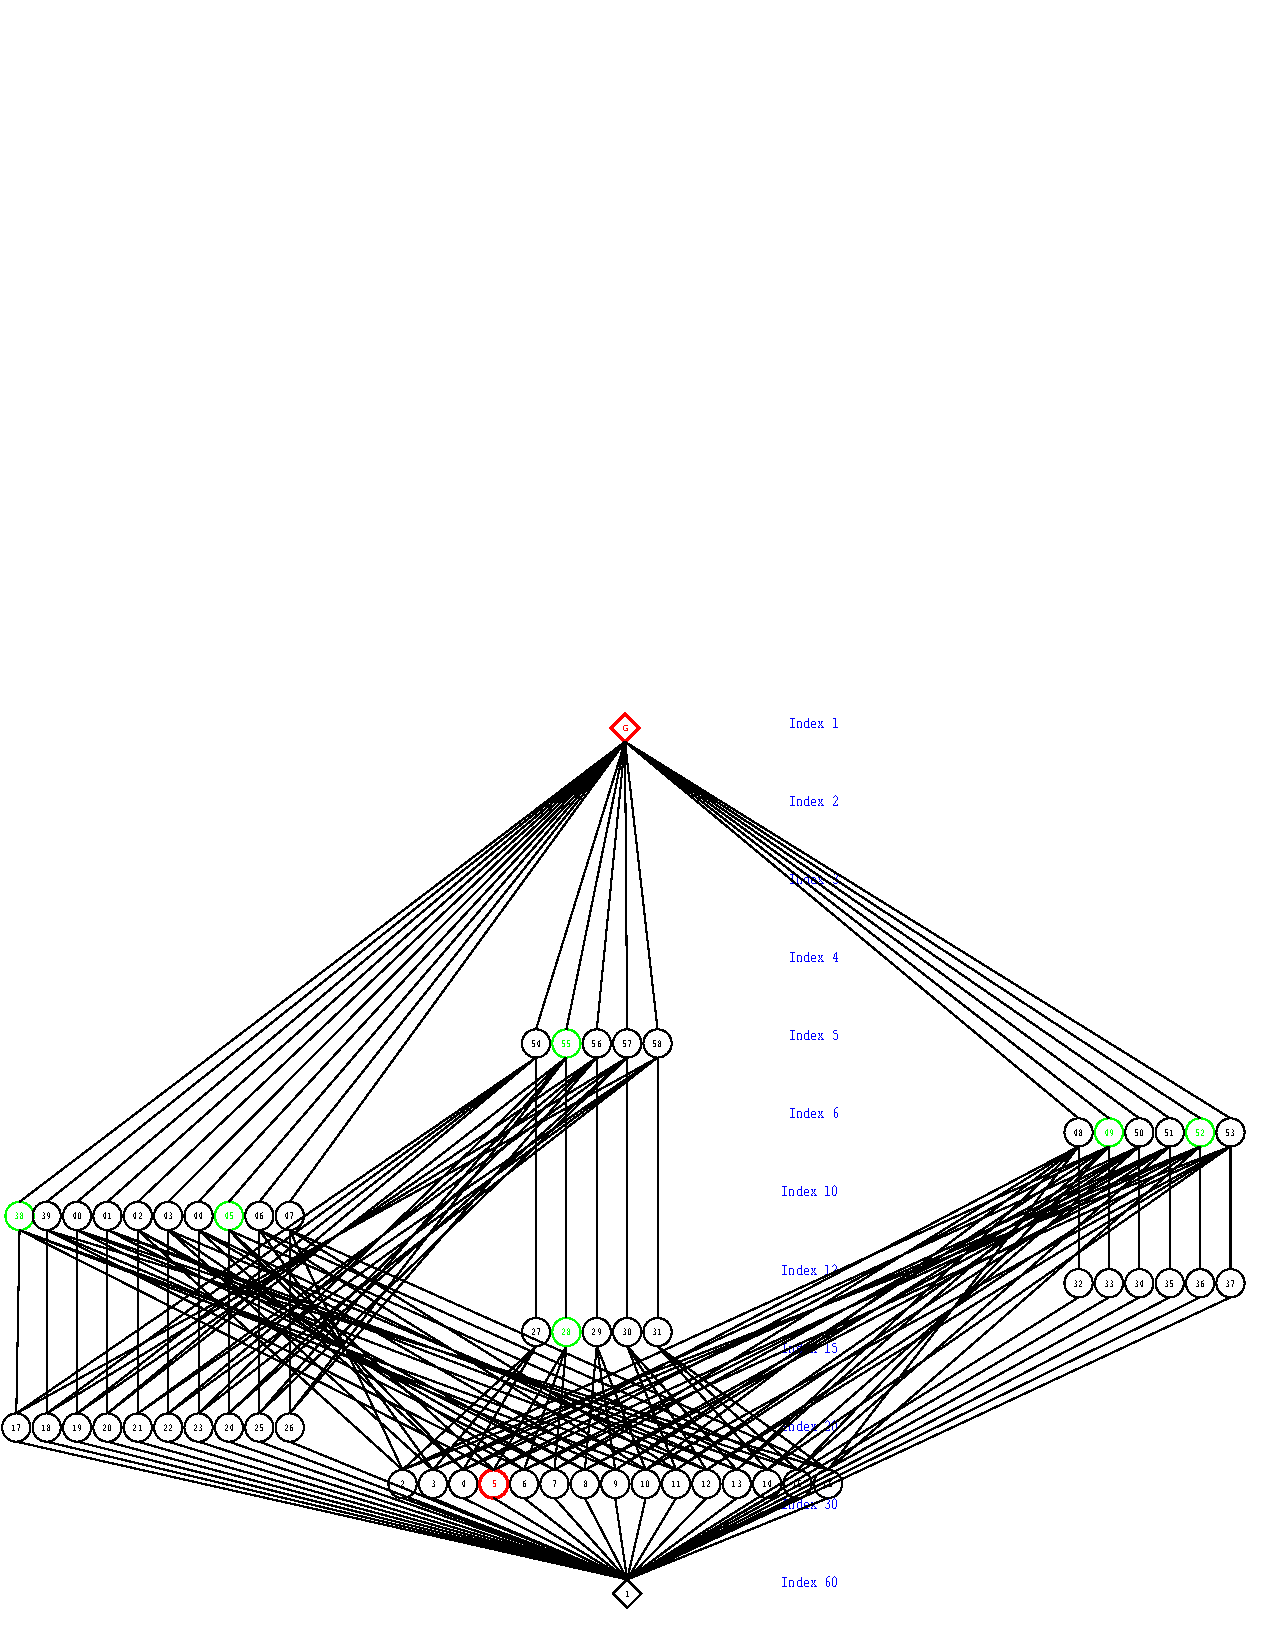
\includegraphics[height=15cm]{A5UpperN5.pdf}%
\caption{Hasse diagram of $\Sub[A_5]$ drawn by the \xgap\ program. Colored green are the
subgroups in the interval above one of the $\Z_2$ subgroups of $A_5$.  Thus,
$A_5$ acts transitively on the 30 cosets of $\Z_2$, and the
permutational algebra $\<A_5/\Z_2; A_5\>$ has congruence lattice isomorphic to 
the interval $[\Z_2, A_5]$.}
\label{fig:A5new}
\end{center}
\end{figure}

If we use the \xgap\ program as described above we could count the conjugacy classes of subgroups by
looking at the Hasse diagram of $\Sub[A_5]$.  However, it's more convenient (and
faster) to simply do: 
{\codesize 
\begin{verbatim}
gap> ccsg := ConjugacyClassesSubgroups( a5 );;
gap> Size(ccsg);
\end{verbatim}}
\noindent which returns 9, telling us that $A_5$ has 9 conjugacy classes of subgroups.  
This includes the singleton classes $\{(e)\}$ and $\{A_5\}$,
which \gap\ calls \verb!Group( () )^G! and \verb!AlternatingGroup( [ 1 .. 5 ] )^G!,
respectively. 
Let's examine the other seven classes.  We get a list of representative subgroups, one for
each class, as follows:
{\codesize 
\begin{verbatim}

gap> clreps := List( ccsg, x -> Representative( x ));
[ Group(()), Group([ (2,3)(4,5) ]), Group([ (3,4,5) ]), 
  Group([ (2,3)(4,5), (2,4)(3,5) ]), Group([ (1,2,3,4,5) ]), 
  Group([ (3,4,5), (1,2)(4,5) ]), Group([ (1,2,3,4,5), (2,5)(3,4) ]), 
  Group([ (2,3)(4,5), (2,4)(3,5), (3,4,5) ]), Alt( [ 1 .. 5 ] ) ]

\end{verbatim}}
\noindent The orders and indices of these subgroups are given by
{\codesize 
\begin{verbatim}

gap> List( clreps, x -> Order(x));         
     % returns [ 1, 2, 3, 4, 5, 6, 10, 12, 60 ]
gap> List( clreps, x -> Index( a5, x ) );  
     % returns [ 60, 30, 20, 15, 12, 10, 6, 5, 1 ]

\end{verbatim}}
\noindent (Of course, any subgroup $H\leq A_5$ has order $|H| = |A_5|\,[A_5:H] = 60 \,[A_5:H]$.)  
From the list of subgroup orders, we see that {\tt clreps[2]}, {\tt clreps[3]},
and {\tt clreps[5]} must be the groups $\Z_2$, $\Z_3$, and $\Z_5$ (the only groups of 
orders two, three, and five, respectively).  
We can easily identify the other subgroups as well.\footnote{A
  nice reference list of all groups of orders 1 through 15 is given on pp.~98--9 of
  Hungerford~\cite{Hungerford:1974}.} 
For example, {\tt clreps[4]} has order 4, so it must be either 
$\Z_2 \oplus \Z_2$ or $\Z_4$.  Deciding to which isomorphism class {\tt clreps[4]}
belongs is simply a matter of checking whether it's cyclic.  These and other
subgroups can be determined using the following \gap\ commands:
% {\tt IsCyclic}, {\tt IsAbelian}, {\tt IsDihedralGroup}, {\tt IsAlternatingGroup}; e.g.
{\codesize 
\begin{verbatim}

gap> IsCyclic( clreps[4] );            # returns false
gap> IsAbelian( clreps[6] );           # returns false
gap> IsDihedralGroup( clreps[6] );     # returns true
gap> IsDihedralGroup( clreps[7] );     # returns true
gap> IsAlternatingGroup( clreps[8] );  # returns true

\end{verbatim}}
\noindent Therefore, {\tt clreps[4]} must be the Klein four group $\Z_2 \oplus
\Z_2$, {\tt clreps[6]} must be $D_3$, 
{\tt clreps[7]}  must be $D_5$.  Finally, {\tt clreps[8]} has
order 12, so it must be one of $\Z_2 \oplus \Z_{6}$, $\Z_{12}$, $A_4$,
$D_6$, or %$T$.
the group $T$ (generated by two elements $a, b$ where $|a|=6, b^2 = a^3$, and $ba = a^{-1}b$).  
The last command above shows that {\tt clreps[8]} is $A_4$.

The foregoing demonstrates some useful \gap\ commands, but we could have
identified all these subgroups in one step with the {\tt StructureDescription} command:
{\codesize 
\begin{verbatim}

gap> List(clreps, x->StructureDescription(x));
[ "1", "C2", "C3", "C2 x C2", "C5", "S3", "D10", "A4", "A5" ]

\end{verbatim}}

Now, the representations of $A_5$ are all faithful since $A_5$ is simple.  Below is
a table of all seven (equivalence classes of) permutation representations of
$A_5$ on cosets $A_5/H$, ordered by the number of such cosets (i.e.~the index
$[A_5:H]$): \\
{\small
  \begin{center}
\begin{tabular}{c|c|c|c}
%Conjugacy class & Index & & \\
  Conjugacy & Index & &  \\
   class rep.~$H$   & $[A_5: H]$ & Representation homomorphism & Is it primitive?\\
\hline
$A_4$ &  5 & $\rho_{A_4}  : A_5 \hookrightarrow \Sym(A_5/A_4) \cong S_5$ & yes \\
$D_5$ &  6 & $\rho_{D_5}  : A_5 \hookrightarrow \Sym(A_5/D_5) \cong S_6$ & yes \\
$D_3$ & 10 & $\rho_{D_3}  : A_5 \hookrightarrow \Sym(A_5/D_3) \cong S_{10}$ & yes \\
$\Z_5$& 12 & $\rho_{\Z_5} : A_5 \hookrightarrow \Sym(A_5/\Z_5) \cong S_{12}$ & no\\
$V_4$ & 15 & $\rho_{V_4}  : A_5 \hookrightarrow \Sym(A_5/V_4) \cong S_{15}$ & no\\
$\Z_3$& 20 & $\rho_{\Z_3} : A_5 \hookrightarrow \Sym(A_5/\Z_3) \cong S_{20}$ & no\\
$\Z_2$& 30 & $\rho_{\Z_2} : A_5 \hookrightarrow \Sym(A_5/\Z_2) \cong S_{30}$ & no\\
$(e)$& 60 & $\rho : A_5 \hookrightarrow \Sym(A_5) \cong S_{60}$ & no\\
\hline
\end{tabular}
  \end{center}
  }
~\\[4pt]
We can use \gap\ to verify that $A_5$ does indeed show up as a transitive
subgroup of some of the symmetric groups listed in the table above.  For
example, the first two are checked as follows:
{\codesize 
\begin{verbatim}

gap> NrTransitiveGroups(5);  % returns 5
gap> NrTransitiveGroups(6);  % returns 16
gap> List([1..5], x->StructureDescription(TransitiveGroup(5,x)));
[ "C5", "D10", "C5 : C4", "A5", "S5" ]
gap> List([1..16], x->StructureDescription(TransitiveGroup(6,x)));
[ "C6", "S3", "D12", "A4", "C3 x S3", "C2 x A4", "S4", "S4", "S3 x S3", 
  "(C3 x C3) : C4", "C2 x S4", "A5", "(S3 x S3) : C2", "S5", "A6", "S6" ]

\end{verbatim}}
\noindent The last line above indicates that (some copy of) $A_5$ shows up as a transitive
subgroup of $S_6$.  (Of course, it is \emph{not} the copy of $A_5< S_6$ that
moves only five points!) 

The last column of the table above was filled in simply 
by looking at the subgroup lattice of $A_5$ in~Figure~\ref{fig:A5new}.  
In general, if $H$ is a coatom in $\Sub[G]$ (i.e.~a maximal subgroup of $G$),
then the representation  
\[
\rho_{H} : G \rightarrow \Sym(G/H) \cong S_{[G:H]}
\] is primitive.
\\[10pt]
{\bf G-sets.} Defining G-sets with \gap\ is very useful and important.  It allows us to work
with and analyze a particular permutation representation.  Let us consider the
$A_5$-set given by $A_5$ acting on cosets of $H=$ {clreps[2]} $=C_2$. In \gap\
we do
{\codesize 
\begin{verbatim}

gap> G := AlternatingGroup( 5 );;
gap> ccsg := ConjugacyClassesSubgroups( a5 );;
gap> H := Representative( ccsg[3] );                   # C3
gap> Gbar := Action( G, RightCosets(G,H), OnRight );;  # a subgroup of S20 
                                                       # isomorphic to A5
gap> MovedPoints( Gbar );                              # [ 1, ..., 20 ]
gap> AllBlocks( Gbar );    # [ [ 1, 2, 3, 4 ], [ 1, 6, 11, 16 ], [ 1, 20 ] ]
gap> for b in AllBlocks( Gbar ) do Print( Orbit( Gbar, b, OnSets ), "\n"); od;
\end{verbatim}}
{\scriptsize 
\begin{verbatim}
[ [ 1, 2, 3, 4 ], [ 17, 18, 19, 20 ], [ 13, 14, 15, 16 ], [ 9, 10, 11, 12 ], [ 5, 6, 7, 8 ] ]
[ [ 1, 6, 11, 16 ], [ 2, 7, 12, 17 ], [ 3, 8, 13, 18 ], [ 4, 9, 14, 19 ], [ 5, 10, 15, 20 ] ]
[ [ 1, 20 ], [ 16, 17 ], [ 12, 13 ], [ 11, 18 ], [ 8, 9 ], [ 7, 14 ], [ 6, 19 ], ...
  ..., [ 4, 5 ], [ 3, 10 ], [ 2, 15 ] ]

\end{verbatim}}
\noindent The command {\tt MovedPoints} shows that {\tt Gbar} $\cong A_5$ acts transitively on the set
$G/H = A_5/Z_3$ of 30 cosets.  (We could also have checked that the action is transitive
using {\tt Orbits(Gbar)} and noting that there is just one orbit.)
The command {\tt AllBlocks(Gbar)} shows 
the first block of each nontrivial ``system of imprimitivity'' (or congruence) of
the G-set $\<G/H, \bar{G}\>$.  Finally, the last command displays the three
nontrivial congruences, and shows $\Con \<G/H, \bar{G}\>\cong M_3$.  Another way
to see that  $\Con \<G/H, \bar{G}\>\cong M_3$ is to check the sublattice of
intermediate subgroups between $H$ and $G$, as follows:
{\codesize 
\begin{verbatim}
gap> intHG := IntermediateSubgroups(G, H);
\end{verbatim}}
{\codesize
\begin{verbatim}
rec( subgroups := [ Group([(3,4,5), (1,2)(4,5)]), Group([(3,4,5), (2,3)(4,5)]), 
                    Group([(3,4,5), (1,5,3)]) ], 
     inclusions := [[ 0, 1 ], [ 0, 2 ], [ 0, 3 ], [ 1, 4 ], [ 2, 4 ], [ 3, 4 ]] 
   )
\end{verbatim}}
\noindent This results in an object, which I've called {\tt intHG}, having fields
{\tt intHG.subgroups} and {\tt intHG.inclusions}.  The inclusions field shows
the covering relations in the sublattice interval $[H, G] \leq \Sub[G]$.

  % \\[6pt]
% {\bf A more general example.}  The example above was special because $A_5$ is a
% simple group.  In general, given a finite group $G$, and an arbitrary subgroup
% $H$, the representation $\rho_H$ need not be an embedding of $G$ into
% $\Sym(G/H)$.  


\vspace{5mm}
%\noindent {\it Example:\protect\footnotemark  factor groups, natural homs, and representations of
%  normalizers in $A_8$}\\[4pt]
\subsection{Example: $A_8$ factor groups, natural homs, and representations of
  normalizers}\hspace{-2mm}\protect\footnotemark
\footnotetext{From chapter 5 of the \gap\ tutorial~\cite{gaptutorial}.}
The group generated by the permutations (1,2) and (1,2,3,4,5,6,7,8) is $S_8$,
the symmetric group on eight points.  We assign it to the identifier s8 
as follows:
{\codesize
\begin{verbatim}

gap> s8 := Group( (1,2), (1,2,3,4,5,6,7,8) );;

\end{verbatim}}
\noindent Now $S_8$ contains the alternating group on eight points which can be described in
several ways, e.g., as the group of all even permutations in $S_8$, or as the derived
subgroup of $S_8$.
{\codesize
\begin{verbatim}

gap> a8 := DerivedSubgroup( s8 );  
Group([ (1,2,3), (2,3,4), (2,4)(3,5), (2,6,4), (2,4)(5,7), (2,8,6,4)(3,5) ])

gap> Size( a8 );                                  % returns 20160
gap> IsAbelian( a8 );                             % returns false
gap> IsPerfect( a8 );                             % returns true
gap> syl2 := SylowSubgroup( a8, 2 );; 
gap> Size( syl2 );                                % returns 64
gap> Normalizer( a8, syl2 ) = syl2;               % returns true   
                                                  % (Sylow subgroups are self-normalizng.)
gap> cent := Centralizer( a8, Centre( syl2 ) );; 
gap> Size( cent );                                % returns 192
gap> DerivedSeries( cent );; List( last, Size );  % returns [ 192, 96, 32, 2, 1 ]

\end{verbatim}}
\noindent Next we want to calculate a subgroup of $G = $ {\tt a8}, then its normalizer, and finally
the structure of the extension. We begin by forming a subgroup generated by three commuting involutions,
i.e., a subgroup isomorphic to the additive group of the vector space $2^3$.
(We will sometimes refer to this subgroup as $H= $ {\tt elab}.)  
{\codesize
\begin{verbatim}

gap> elab := Group( (1,2)(3,4)(5,6)(7,8), (1,3)(2,4)(5,7)(6,8), (1,5)(2,6)(3,7)(4,8) );;
gap> Size( elab );                                % returns 8
gap> IsElementaryAbelian( elab );                 % returns true

\end{verbatim}}
\noindent As usual, \gap\ prints the group by giving all its generators. This can be annoying, especially if there are
many of them or if they are of huge degree.  You can give a name to the group itself using
the function {\tt SetName}. 
We do this with the name \verb.2^3. below which reflects the mathematical properties of the
group. From now on, \gap\ will use this name when printing the group for us, but we cannot use this
name to specify the group to \gap, because the name does not know to which group it
was assigned.  When talking to the computer, you must always use identifiers.
{\codesize
\begin{verbatim}

gap> SetName( elab, "2^3" ); elab;                    % returns 2^3
gap> norm := Normalizer( a8, elab );; Size( norm );   % returns 1344

\end{verbatim}}
\noindent Now that we have the subgroup $N_G(H)= $ {\tt norm} of order 1344 and its subgroup $H=
$ {\tt elab}, we want to look at its factor
group $N_G(H)/H$. We also want to find preimages of factor group elements, so we use
the {\bf natural homomorphism} defined on $N_G(H)= $ {\tt norm} with kernel $H= $ {\tt
  elab} and image $N_G(H)/H$.
{\codesize
\begin{verbatim}

gap> hom := NaturalHomomorphismByNormalSubgroup( norm, elab );
<action epimorphism>
gap> f := Image( hom );
Group([ (), (), (), (4,5)(6,7), (4,6)(5,7), (2,3)(6,7), (2,4)(3,5),(1,2)(5,6) ])
gap> Size( f );                           % returns 168

\end{verbatim}}
\noindent The factor group {\tt f = } $ N_G(H)/H = $ {\tt norm/elab} is again represented as a permutation
group. 
(However, the action domain of this factor group has nothing to do with the action
domain of {\tt norm}.)
We can now form images and preimages under the natural homomorphism. The set of
preimages of an element under {\tt hom} is a coset modulo $H= $ {\tt elab}. 
%We use the function {\tt PreImages} here because {\tt hom} is not a bijection, 
%so an element of the range can have several preimages or none at all.
{\codesize
\begin{verbatim}

gap> ker:= Kernel( hom );                      % returns  2^3
gap> x := (1,8,3,5,7,6,2);; Image( hom, x );   % returns  (1,7,5,6,2,3,4)
gap> coset := PreImages( hom, last );          % returns  RightCoset(2^3,(2,8,6,7,3,4,5))

\end{verbatim}}
\noindent Note that \gap\ is free to choose any representative for the coset of preimages. Of
course, if $x$ and $y$ are two representatives, the quotient $x^{-1}y$ lies in the
kernel $H= $ {\tt ker} of the homomorphism.
{\codesize
\begin{verbatim}

gap> rep:= Representative( coset );            % returns  (2,8,6,7,3,4,5)
gap> x * rep^-1 in ker;                        % returns  true

\end{verbatim}}
\noindent The factor group $ N_G(H)/H = $ {\tt f} is a \emph{simple} group; i.e., it has no non-trivial normal
subgroups. 
\gap\ can detect this fact, and it can then also find the name by which this simple
group is known among group theorists. (Such names are of course not available for
non-simple groups.)
{\codesize
\begin{verbatim}

gap> IsSimple( f );                              % returns true
gap> IsomorphismTypeInfoFiniteSimpleGroup( f );  
rec( series := "L", parameter := [ 2, 7 ],
name := "A(1,7) = L(2,7) ~ B(1,7) = O(3,7) ~ C(1,7) = S(2,7) ~ 2A(1,7) = U(2,7) ~ A(2,2) = L(3,2)" )
gap> SetName( f, "L_3(2)" );

\end{verbatim}}
\noindent We give {\tt f} the name \verb!L_3(2)! because the last part of the name string reveals that it is isomorphic to the
simple linear group $L_3(2)$. This group, however, also has a lot of other names. 

The group $N_G(H)= $ {\tt norm} acts on the eight elements of its normal subgroup $H
= $ {\tt elab} by conjugation, yielding a representation
of $L_3(2)$ in $S_8$ which leaves one point fixed (namely, the point 1).

More precisely, let $\tau : N_G(H) \rightarrow \Sym(H)$ denote the conjugation
representation (where $\Sym(H)\cong S_8$, since $H$ has 8 elements).  
That is, for each $g\in N_G(H)$, $\tau: g \mapsto \tau_g\in \Sym(H)$,
where $\tau_g(h) = gh g^{-1}$, for $h\in H$.  Now, the kernel
\[
\ker \tau = \{ g\in N_G(H) \mid  gh g^{-1} = h \text{ for all } h\in H\}
\]
clearly contains $H$, since $H$ is abelian.  
%Also, as we saw above, $N_G(H)/H$ is simple, so 
Actually, $\ker \tau$ is equal to $H$.  (Otherwise, $\ker \tau / H$ would
be a nontrivial normal subgroup of $N_G(H)/H$, which is impossible, since $N_G(H)/H$
is simple.)
Therefore, the image of the representation is $\tau(N_G(H)) \cong N_G(H)/H \cong L_3(2)$.  
This image can be computed with the function {\tt Action}, which we will use below.
But first recall that, from the start, we had 
\[
2^3 \cong H \subnormal N_G(H) \leq A_8 \subnormal S_8
\]
and the image $\tau(N_G(H))$ is a subgroup of $\Sym(H) \cong S_8$.  In fact, $\tau(N_G(H)) \leq
N_G(H)$, and we can show that $N_G(H)$ is indeed a split extension of the elementary
abelian group $H$ with the image $\tau(N_G(H))$. 
{\codesize
\begin{verbatim}

gap> op := Action( norm, elab );
Group([ (), (), (), (5,6)(7,8), (5,7)(6,8), (3,4)(7,8), (3,5)(4,6), (2,3)(6,7) ])
gap> IsSubgroup( a8, op );                   % returns true
gap> IsSubgroup( norm, op );                 % returns true
gap> IsTrivial( Intersection( elab, op ) );  % returns true
gap> SetName( norm, "2^3:L_3(2)" );

\end{verbatim}}
\noindent By the way, you should not try the operator \verb.<. instead of the function {\tt IsSubgroup}. Something like
{\codesize
\begin{verbatim}

gap> elab < a8;           % returns false

\end{verbatim}}
\noindent will not cause an error, but the result does not signify anything about the inclusion of one group in another;
\verb.<. tests which of the two groups is less in some total order. On the other hand, the equality operator = in
fact does test the equality of its arguments.

\section{Miscellaneous Useful Commands}
\label{sec:lists}
%\subsection{Lists}
\noindent {\bf Lists.}
A list is constructed as follows:
{\codesize
\begin{verbatim}
gap> mylist := [ 2, 3, 5, 7, 11, 13, 17, 19 ];;
\end{verbatim}}
\noindent You can extract certain elements from a list to generate new lists as follows:
{\codesize
\begin{verbatim}
gap> mylist{[4..6]};     # returns [ 7, 11, 13 ]
gap> mylist{[1,7,1,8]};  # returns [ 2, 17, 2, 19 ]
\end{verbatim}}
\noindent It is possible to nest such sublist extractions, as shown in the following example:
{\codesize
\begin{verbatim}
gap> m := [ [1,2,3], [4,5,6], [7,8,9], [10,11,12] ];; 
gap> m{[1,2,3]}{[3,2]};           # returns [ [ 3, 2 ], [ 6, 5 ], [ 9, 8 ] ]
gap> l := m{[1,2,3]};; l{[3,2]};  # returns [ [ 7, 8, 9 ], [ 4, 5, 6 ] ]
\end{verbatim}}
\noindent Note the difference between the last two outputs.
\\[4pt]
In one of our applications, we constructed a list of lists of intervals
in subgroup lattices.  Here's a simple example:
{\codesize
\begin{verbatim}
gap> G:=SymmetricGroup(5);
gap> H:=Representative(ccsg[8]);   # returns  Group([ (1,2,3,4,5) ])
gap> StructureDescription(H);      # returns  "C5"
gap> intHG:=IntermediateSubgroups(G,H);;
\end{verbatim}}
\noindent The function {\tt IntermediateSubgroups(G,H)} returns an object which has two fields:
{\tt subgroups} containing a lists of the subgroups \emph{strictly} between $H$ and
$G$, and {\tt inclusions} which contains a list of covering relations among the
subgroups in {\tt subgroups}.    For example, if {\tt [ 3, 5 ]} appears in
{\tt inclusions}, it means the subgroup labelled 3 is a maximal subgroup of the
subgroup labelled 5. 
The number 0 denotes $H$ and the highest number denotes $G$.  Continuing with
the example above, we have
{\codesize
\begin{verbatim}
gap> intHG.inclusions;  # returns [ [ 0, 1 ], [ 1, 2 ], [ 1, 3 ], [ 2, 4 ], [ 3, 4 ] ] ]
\end{verbatim}}
\noindent This tells us that the interval from $H=C_5$ up to $G=S_5$ is the lattice of
subgroups shown in the figure below.
\begin{figure}[h]
%\caption{The interval $[C_5, S_5]$ in $\Sub[S_5]$.}
%\label{fig:1}
\begin{center}
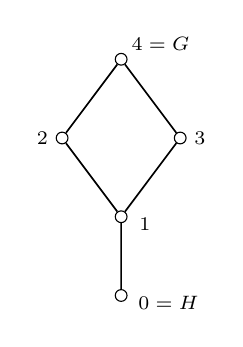
\begin{tikzpicture}[scale=1]
\node (0) at (0,0) [draw, circle,inner sep=1.5pt] {};
\node (1) at (-0,1) [draw, circle, inner sep=1.5pt] {};
\node (2) at (0.75,2) [draw, circle, inner sep=1.5pt] {};
\node (3) at (-0.75,2) [draw, circle, inner sep=1.5pt] {};
\node (4) at (-0,3) [draw, circle, inner sep=1.5pt] {};
\draw[font=\scriptsize] (.6,-.1) node {$0=H$};
\draw[font=\scriptsize] (.5,3.2) node {$4=G$};
\draw[font=\scriptsize] (.3,.9) node {$1$};
\draw[font=\scriptsize] (-1,2) node {$2$};
\draw[font=\scriptsize] (1,2) node {$3$};
\draw[semithick]
(0) to (1)
(1) to (2)
(1) to (3)
(2) to (4)
(3) to (4);
\end{tikzpicture}
\end{center}
\end{figure}

Now, suppose we want to start a list of such covering relation
lists; i.e.~a list of intervals in subgroup lattices. We store the first
interval in {\tt incl}:
{\codesize
\begin{verbatim}
gap> incl:=[intHG.inclusions];  # returns [ [ [ 0, 1 ], [ 1, 2 ], [ 1, 3 ], [ 2, 4 ], [ 3, 4 ] ] ]
\end{verbatim}}
\noindent We get the next interval we want, say,
{\codesize
\begin{verbatim}
gap> K:=Representative(ccsg[10]);;         
gap> intKG:=IntermediateSubgroups(G,K);;
\end{verbatim}}
\noindent Then we use the {\tt Add} function to append the new list of covering relations
to the original list as follows:
{\codesize
\begin{verbatim}
gap> Add(incl,intKG.inclusions);         
gap> incl;
[ [ [ 0, 1 ], [ 1, 2 ], [ 1, 3 ], [ 2, 4 ], [ 3, 4 ] ], 
  [ [ 0, 1 ], [ 0, 2 ], [ 1, 3 ], [ 2, 3 ] ] ]
\end{verbatim}}
\noindent We may want to search all groups for such upper intervals and store them without
repetition.  This is a bit trickier because, for example, GAP views the two lists
{\codesize
\begin{verbatim}
[ [ 0, 1 ], [ 1, 2 ], [ 1, 3 ], [ 2, 4 ], [ 3, 4 ] ],
[ [ 0, 1 ], [ 1, 3 ], [ 1, 2 ], [ 3, 4 ], [ 2, 4 ] ]
\end{verbatim}}
\noindent as distinct, though we recognize them as the same lattice
(shown in the figure above).  This is easily remedied by sorting the lists.  The
first list is already sorted lexicographically.  We sort the second as follows:
{\codesize
\begin{verbatim}
SSortedList([ [ 0, 1 ], [ 1, 3 ], [ 1, 2 ], [ 3, 4 ], [ 2, 4 ] ]);
[ [ 0, 1 ], [ 1, 2 ], [ 1, 3 ], [ 2, 4 ], [ 3, 4 ] ]
\end{verbatim}}
\noindent and see that the sorted version matches the first list.
Unfortunately, not all repetitions of lattice intervals can be avoided simply by
sorting. Consider, for example, the two hexagons,
{\codesize
\begin{verbatim}
[ [ 0, 1 ], [ 0, 2 ], [ 1, 3 ], [ 2, 4 ], [ 3, 5 ], [ 4, 5 ] ]
[ [ 0, 1 ], [ 0, 3 ], [ 1, 2 ], [ 2, 5 ], [ 3, 4 ], [ 4, 5 ] ]
\end{verbatim}}
\noindent These are already sorted, yet they are distinct lists which
give the same lattice.  One solution (perhaps not the most efficient)
is given by the following routine, {\tt isIsomorphicInterval}, which checks
whether two lists of covering relations represent isomorphic intervals;
i.e.~whether they are the same modulo a relabelling of the elements.
{\codesize
\begin{verbatim}

isIsomorphicInterval:=function(list1, list2)
    # Gap function for testing whether two sets of covering relations 
    # are the same modulo relabelling. 
    
    local n, m, j, list3, G, p;
    
    if not IsList(list1) or not IsList(list2) then
        Error("usage: isIsomorphicInterval( <lst1>, <lst2> );");
    fi;
    if Length(list1) <> Length(list2)  then
        return false;
    fi;
        
    list1 := SSortedList(list1);
    list2 := SSortedList(list2);

    n:=Length(list1);
    
    m:=Maximum(Maximum(list1));
  
    G:=SymmetricGroup(m);
    
    for p in Elements(G) do
        list3 := [[ ]];
        for j in [1..n] do
            list3[j]:=List(list1[j], x->((x+1)^p)-1); 
        od;
        list3:=SSortedList(list3);
        if list3=list2 then
            return true;
        fi;
    od;
    return false;
end;

\end{verbatim}}


\newpage


\section{Citing This Document}
Please use the following BibTeX data to cite this document.



{\small
\begin{verbatim}
  @unpublished{DeMeo:2017,
  author    = {William DeMeo},
  title     = {{F}acts on {F}inite {G}roups:
    a smorgasbord of known results, experimental data and other trivia},
  year      = {2017},
  note      = {Available at: 
         \url{https://arxiv.org/find/math/1/au:+DeMeo_W/0/1/0/all/0/1}},
  url       = {https://arxiv.org/find/math/1/au:+DeMeo_W/0/1/0/all/0/1}
  }
\end{verbatim}
}
%%%%%%%%%%%%%%%%%%%%   End of main body of article
%
%                             References
%
%   BiBTeX users uncomment the following line:
%
\bibliographystyle{plainurl} %jloganal}
%
\bibliography{refs}

%%%%%%%%%%% TOTO: Insert bibtex data here!! %%%%%%%%%%%%%%%%%%5

\end{document}


